%\documentclass[11pt]{report}
\documentclass[11pt,twoside]{report}

\usepackage{graphicx}
\usepackage{url}
\usepackage[bf]{caption}
%\usepackage{enumitem}
\usepackage{array}
\newcolumntype{L}{>{\centering\arraybackslash}m{3cm}}
\usepackage{tikz}
%\usepackage[textsize=scriptsize,colorinlistoftodos]{todonotes}
\usepackage{verbatim}
\usepackage [T1]{fontenc}
\usepackage[utf8]{inputenc}
\usepackage[inline]{enumitem}
\usepackage{multirow}
\usepackage{polski}
\usepackage{amssymb}
\usepackage{amsmath}
\usepackage{pdflscape}
\usepackage[left=3.5cm,top=2.5cm,bottom=2.5cm,right=2cm]{geometry}
\linespread{1.5}
\usepackage{lipsum}
\usepackage{longtable}
\usepackage[]{hyperref}
\hypersetup{
%    bookmarks=true,         % show bookmarks bar?
    unicode=true,          % non-Latin characters in Acrobat’s bookmarks
    pdftoolbar=true,        % show Acrobat’s toolbar?
    pdfmenubar=true,        % show Acrobat’s menu?
    pdffitwindow=false,     % window fit to page when opened
    pdfstartview={FitH},    % fits the width of the page to the window
%    pdftitle={},    % title
%    pdfauthor={},     % author
    %pdfsubject={},   % subject of the document
    %pdfcreator={Creator},   % creator of the document
    %pdfproducer={Producer}, % producer of the document
%    pdfkeywords={}, % list of keywords
    pdfnewwindow=true,      % links in new window
    colorlinks=true,       % false: boxed links; true: colored links
    linkcolor=black,          % color of internal links
    citecolor=black,        % color of links to bibliography
    filecolor=black,      % color of file links
    urlcolor=black,           % color of external links
}

%biblioigrafia
\usepackage[sort&compress]{natbib}
\bibpunct{[}{]}{;}{a}{}{,}
\renewcommand{\cite}{\citep}

\usepackage{amssymb}
\renewcommand{\baselinestretch}{1.5} 
\usepackage{listings}

\lstset{frame=tb,
  language=Java,
  aboveskip=3mm,
  belowskip=3mm,
  showstringspaces=false,
  columns=flexible,
  basicstyle={\small\ttfamily},
  numbers=none,
  breaklines=true,
  breakatwhitespace=true,
  tabsize=3
}
%%%%%%%%%%%%%%%%%%%%%%%%%%%%%%%%%%%%%%%%%
% Minimalist Book Title Page 
% LaTeX Template
% Version 1.0 (27/12/12)
%
% This template has been downloaded from:
% http://www.LaTeXTemplates.com
%
% Original author:
% Peter Wilson (herries.press@earthlink.net)
%
% License:
% CC BY-NC-SA 3.0 (http://creativecommons.org/licenses/by-nc-sa/3.0/)
% 
% Instructions for using this template:
% This title page compiles as is. If you wish to include this title page in 
% another document, you will need to copy everything before 
% \begin{document} into the preamble of your document. The title page is
% then included using \titleTH within your document.
%
%%%%%%%%%%%%%%%%%%%%%%%%%%%%%%%%%%%%%%%%%

%----------------------------------------------------------------------------------------
%	PACKAGES AND OTHER DOCUMENT CONFIGURATIONS
%----------------------------------------------------------------------------------------
%
%\documentclass{book}
%
%\usepackage[svgnames]{xcolor} % Required to specify font color
%
%\newcommand*{\plogo}{\fbox{$\mathcal{PL}$}} % Generic publisher logo

%----------------------------------------------------------------------------------------
%	TITLE PAGE
%----------------------------------------------------------------------------------------

\newcommand*{\titleTH}{\begingroup % Create the command for including the title page in the document

\thispagestyle{empty}

\begin{center}
  \makebox[\textwidth]{
\includegraphics[width=\paperwidth]{header.png}}
\end{center}

\raggedleft % Right-align all text
\vspace*{\baselineskip} % Whitespace at the top of the page

{\LARGE mgr Łukasz Wawrowski}\\ % Author name
\vspace{15mm}
{{\huge Estymacja pośrednia ubóstwa na poziomie regionalnym i lokalnym w Polsce}}\\[\baselineskip] % Tytuł w języku polskim
{{\huge Indirect estimation of poverty at the regional and local level in Poland}}\\ % Tytuł w języku angielskim
\vspace{20mm}
{\Large Praca doktorska}\\
\vspace{20mm}

{\Large Promotor: dr hab. Grażyna Dehnel, prof. nadzw. UEP}\\
%{\Large Pracę przyjęto dnia ...................}\\
\vspace{45mm}

%\small{podpis Promotora}

\raggedright
Wydział Informatyki i Gospodarki Elektronicznej\\
Katedra Statystyki

\vspace*{3\baselineskip} % Whitespace at the bottom of the page
\endgroup}

%----------------------------------------------------------------------------------------
%	BLANK DOCUMENT
%----------------------------------------------------------------------------------------
%
%\begin{document} 
%
%\pagestyle{empty} % Removes page numbers
%
%\titleTH % This command includes the title page
%
%\end{document}


\usepackage{polski}
\usepackage{adjustbox}
\usepackage[utf8]{inputenc}
\usepackage{amsmath}
\usepackage{emptypage}

\usepackage{afterpage}

\newcommand\blankpage{%
    \null
    \thispagestyle{empty}%
    \addtocounter{page}{-1}%
    \newpage}

\title{Doktorat}
\author{Łukasz Wawrowski}
\date{Data}

\begin{document}

\pagenumbering{Roman}

\titleTH % Nowa strona tytulowa zgodnie z wymogami

\cleardoublepage
%\afterpage{\blankpage}

%\chapter*{Podziękowania}

\tableofcontents

\cleardoublepage
\addcontentsline{toc}{chapter}{Spis rysunków}
\listoffigures

\cleardoublepage 
\addcontentsline{toc}{chapter}{Spis tabel}
\listoftables

\cleardoublepage 
\addcontentsline{toc}{chapter}{Wykaz skrótów}

\chapter*{Wykaz ważniejszych skrótów}

\begin{description}[leftmargin=8em,style=nextline,itemsep=0pt]
\item[HT] estymator Horvitza-Thompsona
\item[BLUP] najlepszy liniowy nieobciążony predyktor (ang. \textit{Best Linear Unbiased Predictor})
\item[EBLUP] empiryczny najlepszy liniowy nieobciążony predyktor (ang. \textit{Empirical Best Linear Unbiased Predictor})
\item[SEBLUP] przestrzenny empiryczny najlepszy liniowy nieobciążony predyktor (ang. \textit{Spatial Empirical Best Linear Unbiased Predictor})
\item[EB] metoda Empiryczna Bayesowska (ang. \textit{Empirical Bayes})
\item[MQ] metody M-kwantylowa (ang. \textit{M-quantile})
\item[FH] model Faya-Herriota
\item[SFH] przestrzenny model Faya-Herriota
\item[SE] błąd standardowy (ang. \textit{Standard Error})
\item[MSE] błąd średniokwadratowy (ang. \textit{Mean Square Error})
\item[RRMSE] względny pierwiastek błędu średniokwadratowego (ang. \textit{Relative Root Mean Square Error})
\item[SAMPLE] Small Area Methods for Poverty and Living Condition Estimates
\item[AMELI] Advanced Methodology for European Laeken Indicators
\item[SAIPE] Small Area Income and Poverty Estimates
\item[NSP] Narodowy Spis Powszechny Ludności i Mieszkań
\item[EU-SILC] Europejskie Badanie Dochodów i Warunków Życia
\item[BBGD] Badanie Budżetów Gospodarstw Domowych
\item[BSS] Badanie Spójności Społecznej
\item[DS] Diagnoza Społeczna
\item[BDL] Bank Danych Lokalnych
\end{description}

\cleardoublepage 
\addcontentsline{toc}{chapter}{Wykaz symboli}

\chapter*{Wykaz ważniejszych symboli}

\begin{description}[leftmargin=8em,style=nextline,itemsep=0pt]
\item[$U$] populacja
\item[$j$] jednostka
\item[$s$] zbiór jednostek wylosowanych z populacji $U$
\item[$r$] zbiór jednostek niewylosowanych z populacji $U$
\item[$N$] liczebność populacji
\item[$n$] liczebność próby
\item[$d$] domena, mały obszar
\item[$N_d$] liczebność populacji w domenie
\item[$n_d$] liczebność próby w domenie
\item[$\theta$] wartość parametru
\item[$\hat{\theta}$] oszacowanie parametru
\item[$Y$] wartość globalna zmiennej badanej
\item[$E_{dj}$] wartość dochodu $j$-tej jednostki w $d$-tej domenie
\item[$z$] granica ubóstwa
\item[$F_{\alpha}$] wskaźnik ubóstwa
\item[$\psi$] wariancja z próby
\item[$\boldsymbol{x}$] macierz zmiennych objaśniających
\item[$\beta$] wektor parametrów efektów stałych
\item[$u$] wektor efektów losowych
\item[$e$] wektor reszt/błędów losowych
\item[$W$] macierz sąsiedztwa
\item[$\Psi$] funkcja wpływu
\end{description}

\clearpage
\pagenumbering{arabic}

\chapter*{Wstęp}
\addcontentsline{toc}{chapter}{Wstęp}
Ubóstwo jest uznawane za jeden z najważniejszych i najbardziej złożonych problemów społecznych współczesnego świata. Zjawisko to występuje w każdym społeczeństwie. W niektórych krajach jest ono bardziej widoczne, w innych mniej. Niekoniecznie oznacza to jednak, że różnią się one zasięgiem ubóstwa. Mamy bowiem tu do czynienia z pojęciem zróżnicowanym terytorialnie. Bieda osób mieszkających w Europie znacznie różni się od tej, która dotyka mieszkańców krajów Afryki, czy Azji. Poza wyżej wskazanym wymiarem przestrzennym, ważnym przy określaniu poziomu, czy głębokości ubóstwa jest także wymiar czasowy. Jedną z konsekwencji procesu rozwoju społeczeństwa jest bowiem zmieniający się w czasie status materialny gospodarstwa domowego. Kluczowym problemem zatem w ocenie ubóstwa jest jego pomiar. Nadanie mu uniwersalnego charakteru wymagałoby określenia jednolitych zasad i definicji stanowiących podstawę kryterium wyróżnienia sfery ubóstwa. Jest to jednak bardzo trudne zadanie, którego jak dotąd nie udało się zrealizować.

W przeszłości wielu badaczy podejmowało problem zdefiniowania zjawiska niedostatku. Można w tym miejscu przywołać polskiego ekonomistę, profesora Jana Drewnowskiego, który łączył ubóstwo z niezaspokojeniem potrzeb na oczekiwanym poziomie \citep{drewnowski1977}. Z kolei Amartya Sen, indyjski ekonomista i laureat Nagrody Banku Szwecji im. Alfreda Nobla, wskazał, że ubóstwo to nie tylko niedostępność określonych dóbr i usług, ale także brak możliwości uczestnictwa w podejmowaniu decyzji oraz udziału w życiu społecznym i kulturalnym \citep{sen1992}. Rada Europejskiej Wspólnoty Gospodarczej (WE) w dokumencie z dnia 19 grudnia 1984 roku w sprawie działań mających na celu przeciwdziałanie ubóstwu zdefiniowała to zjawisko w następujący sposób: ,,ubóstwo odnosi się do osób, rodzin lub grup osób, których zasoby (materialne, kulturowe i społeczne) są ograniczone w takim stopniu, że poziom ich życia obniża się poza akceptowalne minimum w kraju zamieszkania'' \citep{eec1985}.

W definicji określonej przez Radę Europejskiej Wspólnoty Gospodarczej kluczowym aspektem jest ustalenie kryterium przynależności do sfery ubóstwa. Wyróżnia się tu dwa wiodące podejścia do zagadnienia: jednowymiarowe lub wielowymiarowe. Stosując kryterium jednowymiarowe ocenia się stopień zaspokojenia potrzeb jednostki poprzez pryzmat dochodów (wydatków) wyrażonych jedynie w formie monetarnej. W literaturze przedmiotu podkreślana jest jednak niedoskonałość tego podejścia oraz przekonanie, że zjawisko ubóstwa nie jest jednowymiarowe \citep{panek2010,jakosc-gus2013}. W~związku z tym wielu badaczy zaczęło postulować o uwzględnienie w jego analizie także czynników pozamonetarnych. Wśród propozycji wymiarów ubóstwa, które miałyby zostać włączone do analizy znalazły się m.in. dochody i zasoby materialne nagromadzone w~poprzednich okresach, warunki mieszkaniowe, edukacja oraz zasoby zawodowe i finansowe \citep{panek2011}. 

Pomimo swoich ograniczeń podejście jednowymiarowe jest wykorzystywane w badaniach prowadzonych przez Główny Urząd Statystyczny (GUS) ze względu na prostotę obliczeń, w których wykorzystuje się wartości wyłącznie jednej cechy --- dochodów bądź wydatków \citep{ubostwo-gus2013}. 

Stosowanie podejścia jednowymiarowego wymaga określenia poziomu dochodów (wydatków), poniżej którego osoba jest uznawana za ubogą. W Polsce zdefiniowanych jest kilka rodzajów granicy (linii) ubóstwa. Instytut Pracy i Spraw Socjalnych (IPiSS) wyznacza wartości: minimum egzystencji (granicę wydatków uwzględniających skromne wyżywienie oraz utrzymanie małego mieszkania), minimum socjalne (granicę wydatków umożliwiającą minimalnie godziwy standard życia), a także bierze udział w konsultacji ustawowej granicy ubóstwa (kwoty dochodu, która uprawnia do ubiegania się przyznanie świadczenia z systemu pomocy społecznej) \citep{kurowski2002}. W badaniach społecznych granicę ubóstwa ustala się jako stałą część mediany lub średniej arytmetycznej rozkładu dochodów w całej populacji. GUS w Badaniu Budżetów Gospodarstw Domowych (BBGD) wykorzystuje linię ubóstwa określoną jako 50\% średnich wydatków. Z kolei Eurostat rekomenduje przyjęcie jako granicy ubóstwa 60\% mediany rozkładu dochodów ekwiwalentnych (uwzględniających skład demograficzny gospodarstwa domowego). 

Pomiar niedostatku bazuje na dwóch podstawowych wskaźnikach: \textit{stopie ubóstwa} oraz \textit{głębokości ubóstwa}. Pierwsza z tych miar informuje o odsetku ubogich w populacji. Wskaźnik ten jest prosty w budowie i interpretacji, niemniej posiada kilka wad. Przede wszystkim, nie bierze pod uwagę intensywności ubóstwa --- osoby znajdujące się poniżej granicy ubóstwa mogą mieć dochody bardzo zbliżone do tej granicy lub bardzo oddalone. W obu przypadkach stopa ubóstwa będzie taka sama, natomiast niewątpliwie większa bieda występuje w drugiej sytuacji. Uzupełnieniem stopy ubóstwa jest głębokość ubóstwa, która informuje o poziomie ubóstwa wśród osób znajdujących się poniżej linii ubóstwa. Oznacza to zatem, że pełniejszy obraz zjawiska otrzymamy prowadząc analizę opartą na obu wymienionych wskaźnikach \citep{haughton2009}.

Badania empiryczne prowadzone w Polsce dostarczają informacji na temat biedy na bardzo ogólnym poziomie. Głównym źródłem oszacowań wskaźników ubóstwa są badania reprezentacyjne prowadzone przez GUS takie jak Badanie Budżetów Gospodarstw Domowych (BBGD) oraz Europejskie Badanie Dochodów i Warunków Życia (EU-SILC). Jak dotąd wartości wskaźników ubóstwa publikowane są na poziomie całego kraju, w przekroju regionów oraz wybranych grup społeczno-demograficznych. Wielkość próby, jak również wykorzystywana obecnie metoda szacunku jaką jest estymacja bezpośrednia nie pozwalają na publikację wyników na niższych poziomach agregacji z powodu wysokich błędów oszacowań. Ponadto z roku na rok coraz więcej osób odmawia udziału w badaniach reprezentacyjnych \citep{dezagregacja2015}. Równolegle do obserwowanych spadków wskaźników realizacji badań reprezentacyjnych rosną potrzeby odbiorców informacji. Oczekuje się danych dla szczegółowych przekrojów oraz coraz mniejszych jednostek administracyjnych czy terytorialnych.

Rozszerzenie pokrycia informacyjnego bez konieczności zwiększenia kosztów badania wynikających między innymi ze zmiany wielkości próby jest możliwe poprzez zastosowanie metod statystyki małych obszarów (estymacji pośredniej). Są to techniki umożliwiające estymację parametrów przy ograniczonej, w skrajnym przypadku zerowej, liczebności próby, wykorzystując w tym celu wszystkie dostępne źródła danych. Ten typ estymacji ma bardzo szerokie spectrum zastosowań. Oprócz badań nad ubóstwem \citep{ell2003,ebp2010,mq2006,esteban2012,pratesi2008}, metody statystyki małych obszarów wykorzystuje się między innymi w szacowaniu charakterystyk rynku pracy \citep{golata2004,wilak2014,molina2007}, niepełnosprawności \citep{elazar2004} oraz w statystyce gospodarczej \citep{dehnel2010,dehnel2017,chandra2012}.

W rozprawie do estymacji wskaźników ubóstwa na poziomie podregionów i powiatów zostaną wykorzystane dwa typy modeli: obszarowe oraz jednostkowe. Bazują one na estymacji danej zmiennej zależnej za pomocą liniowego modelu mieszanego --- zawierającego efekt losowy przyporządkowany zazwyczaj do określonego stopnia podziału administracyjnego \citep{rao2015}. 

Otrzymane wyniki będą mogły stanowić składową obrazu spójności społecznej Polski w ujęciu regionalnym i~lokalnym. Efektem przeprowadzonego badania będą kartogramy na poziomie NUTS 3 i NUTS 4 umożliwiające identyfikację obszarów najbardziej narażonych na występowanie zjawiska ubóstwa. Z kolei wypracowana metodyka może zostać wykorzystana jako narzędzie ewaluacji w prowadzonych obecnie przedsięwzięciach takich jak \textit{Europa 2020}, \textit{Krajowy Program Reform}, \textit{Agenda Post-2015} czy \textit{Krajowy Program Przeciwdziałaniu Ubóstwu i Wykluczeniu Społecznemu 2020. Nowy wymiar aktywnej integracji} mających na celu zmniejszenie poziomu ubóstwa. Wnioski uzyskane na podstawie przeprowadzonych badań będą mogły służyć jako informacja dla władz samorządowych w kontekście planowania efektywnej polityki społecznej.

\subsection*{Cel pracy}

Głównym celem rozprawy jest \textbf{pomiar ubóstwa na poziomie podregionów i powiatów w~Polsce} z wykorzystaniem statystyki małych obszarów. Szacowaniu podlega stopa oraz głębokość ubóstwa w 2011 roku dla wyżej wymienionych przekrojów. 

Osiągnięcie celu głównego będzie możliwe poprzez realizację kolejnych celów szczegółowych:

\begin{itemize}
\item określenie stanu wiedzy dotyczącej pokrycia informacyjnego wskaźników ubóstwa oraz metod estymacji tych wskaźników,
\item charakterystyka i ocena źródeł danych wykorzystywanych w estymacji ubóstwa,
\item analiza potencjalnych źródeł zmiennych pomocniczych, w tym zasobów wykraczających poza tradycyjne bazy danych,
\item adaptacja metod estymacji wskaźników ubóstwa na poziomie podregionów i powiatów w~Polsce wykorzystujących podejście modelowe,
\item statystyczna ocena szacunków pod kątem precyzji i obciążenia,
\item przestrzenna analiza oszacowań wskaźników ubóstwa na poziomie podregionów i powiatów w~Polsce,
\item wyodrębnienie jednostek terytorialnych o podobnych wartościach wskaźników ubóstwa,
\item zastosowanie metod wielowymiarowej analizy statystycznej w ocenie oszacowań wskaźników ubóstwa.
\end{itemize}

\subsection*{Hipotezy badawcze}

W związku z realizacją celów postawionych w rozprawie sformułowano trzy hipotezy badawcze.

\begin{enumerate}
\item Ubóstwo ekonomiczne cechuje się wyraźnym zróżnicowaniem przestrzennym na poziomie lokalnym w Polsce.
\item Estymacja poziomu ubóstwa wykorzystująca zmienne pomocnicze z innych źródeł charakteryzuje się lepszą jakością w porównaniu do estymacji bezpośredniej.
\item Związek pomiędzy poziomem ubóstwa mierzonym stopą i głębokością ubóstwa, a sytuacją na rynku pracy jest wyraźniejszy w ujęciu lokalnym niż w przekroju podregionów.
\end{enumerate}

W polskiej literaturze przedmiotu brakuje kompleksowych analiz poświęconych problematyce estymacji pośredniej wskaźników ubóstwa w ujęciu regionalnym i lokalnym. Ujęcie to zostało podniesione w rozprawie stanowiąc \textbf{novum pracy}. Pomimo wielu opracowań poruszających kwestie ubóstwa, rzadkie są prace dotyczące estymacji zarówno stopy, jak i głębokości ubóstwa. Za oryginalny wkład rozprawy uznać można w pierwszym rzędzie adaptację metod pośrednich wykorzystywanych w badaniu ubóstwa na świecie do ram polskiego systemu statystyki publicznej. Oryginalnym wkładem jest również przedstawienie terytorialnego zróżnicowania głębokości ubóstwa w przekroju podregionów i powiatów w oparciu o przeprowadzoną estymację. Na podkreślenie zasługuje również zawarta w pracy ocena uzyskanych oszacowań, która ma charakter wielopłaszczyznowy. Wykorzystano w niej dostępne informacje pochodzące z rejestrów administracyjnych oraz metody wielowymiarowej analizy statystycznej.

\subsection*{Charakterystyka zastosowanych metod badawczych}

W pracy podjęto próbę estymacji wskaźników ubóstwa na poziomie podregionów i powiatów z~wykorzystaniem modeli statystyki małych obszarów. Jako zmienną zależną przyjęto wskaźnik ubóstwa mierzony na określonym poziomie terytorialnym (w podejściu obszarowym) lub dochód gospodarstwa (w podejściu jednostkowym). Po drugiej stronie równania jako zmienne niezależne przyjęto tzw. \textit{zmienne pomocnicze} --- informacje silnie skorelowane ze zmienną zależną pochodzące z dodatkowego źródła danych.

W badaniu kluczową rolę przy budowie modelu wykorzystanego w estymacji, odegrała identyfikacja symptomów ubóstwa. Pełniły one w procesie modelowania rolę informacji pomocniczej. Wskazanie cech stanowiących determinanty ubóstwa pozwoliło na stworzenie bazy tzw. \textit{zmiennych pomocniczych}. Wśród najistotniejszych symptomów ubóstwa znalazły się takie cechy jak: źródło utrzymania gospodarstwa, liczebność gospodarstwa, wykształcenie członków gospodarstwa domowego czy występowanie w nim osób bezrobotnych bądź niepełnosprawnych.

W modelach obszarowych poziom analizowanego wskaźnika ubóstwa w danym obszarze objaśniany jest zmiennymi mierzonymi na poziomie tego obszaru. Wykorzystuje się w tym celu charakterystyki społeczno-ekonomiczne dostępne w powszechnych bazach statystycznych takich jak np. Bank Danych Lokalnych. Przykładowo poziom stopy ubóstwa w danym powiecie może być wyjaśniony przez odsetek osób nieposiadających wyższego wykształcenia w tym powiecie. Możliwość wykorzystania bogatszego zbioru zmiennych pomocniczych, w porównaniu z podejściem jednostkowym, stanowi bardzo ważną zaletę modeli obszarowych. Najpopularniejszym przedstawicielem tej grupy metod jest model Faya-Herriota opracowany w celu szacowania średniego dochodu w małych domenach w Stanach Zjednoczonych \citep{fh1979}. Podejście to jest cały czas rozwijane m.in. poprzez ujęcie w modelu macierzy sąsiedztwa i uwzględnienie w ten sposób czynnika przestrzennego \citep{pratesi2008}. To rozszerzenie charakteryzuje się lepszymi własnościami, niż klasyczny model Faya-Herriota, ale wymaga spełnienia dodatkowych założeń, takich jak występowania istotnej korelacji przestrzennej.

Modele jednostkowe z kolei bazują na modelowaniu dochodów lub wydatków gospodarstw domowych z wykorzystaniem danych jednostkowych pochodzących z badań pełnych lub rejestrów administracyjnych. W tym przypadku dostępność zmiennych niezależnych jest dużo mniejsza od tej, występującej dla modeli obszarowych z powodów wynikających między innymi z~zachowania tajemnicy statystycznej. Dochód gospodarstwa domowego może być objaśniany przez charakterystyki tego gospodarstwa takie jak: liczba osób bezrobotnych czy wskaźnik obciążenia demograficznego. Do najważniejszych technik estymacji opartych na modelach jednostkowych należą metody ELL \citep{ell2003}, M-kwantylowa (MQ) \citep{mq2006} oraz empiryczna bayesowska (EB) \citep{ebp2010}. Estymacja danego wskaźnika ubóstwa w przypadku tych metod polega na tworzeniu, z~wykorzystaniem symulacji Monte Carlo, pseudo-populacji, które stanowią podstawę estymacji wskaźników ubóstwa. Wymienione metody są do siebie bardzo podobne jeśli chodzi o ideę. Dzielą je jednak istotne różnice. Metoda ELL nie uwzględnia bowiem w ogóle danych pochodzących z badania reprezentacyjnego w przeciwieństwie do metody EB. Z~kolei w metodzie MQ liniowy model mieszany został zastąpiony przez model regresji kwantylowej.

W dysertacji zastosowano wyżej przedstawione modele do estymacji stopy oraz głębokości ubóstwa na poziomie podregionów i powiatów. Rozważano także różne metody transformacji zmiennej zależnej, które miały na celu poprawę własności predykcyjnych modeli \citep{analpovdata52016}. Obciążenie oraz precyzja wszystkich otrzymanych szacunków zostały ocenione za pomocą metody bootstrap \citep{gonzales2008}. Na tej podstawie dokonano wyboru najlepszej metody estymacji w odniesieniu do danego poziomu terytorialnego.

Wszystkie obliczenia oraz wizualizacje zostały wykonane w pakiecie R \citep{r2016}.

\subsection*{Źródła danych}

Do estymacji poziomu ubóstwa w Polsce zastosowano dane jednostkowe z Europejskiego Badania Dochodów i Warunków Życia (EU-SILC) z roku 2011. Wybór tego okresu analizy podyktowany został dostępnością danych statystycznych wykorzystanych w estymacji pośredniej w charakterze \textit{zmiennych pomocniczych}. Ich źródło stanowiły informacje zebrane w ramach Narodowego Spisu Powszechnego Ludności i Mieszkań przeprowadzonego w 2011 roku. Oprócz tego wspomagano się danymi pochodzącymi z Banku Danych Lokalnych. 

\subsection*{Treść pracy}

Praca ma charakter teoretyczno-empiryczny i składa się ze wstępu, pięciu rozdziałów, zakończenia, bibliografii oraz załączników. Pierwsze trzy rozdziały mają charakter teoretyczny, a ich podstawą są badania literaturowe. Z kolei czwarty i piąty rozdział zawiera wyniki przeprowadzonych badań empirycznych --- oszacowania stopy oraz głębokości ubóstwa na poziomie podregionów i~powiatów wraz z ich statystyczną oraz merytoryczną oceną.

W \textbf{rozdziale pierwszym} zostały przedstawione teoretyczne aspekty pomiaru ubóstwa. Na podstawie literatury przedmiotu zidentyfikowano najważniejsze determinanty ubóstwa. W treści rozdziału poświęcono także miejsce na przegląd projektów badawczych dotyczących statystycznej analizy ubóstwa. Duża liczba takich inicjatyw świadczy o aktualności problemu badawczego. Ponadto w rozdziale, na podstawie dostępnych źródeł przedstawiono czasowy oraz przestrzenny wymiar ubóstwa w Polsce. 

\textbf{Rozdział drugi} zawiera opis źródeł danych wykorzystywanych w badaniu ubóstwa. Uwagę skupiono w pierwszej kolejności na źródłach, na których obecnie oparte są publikacje dotyczące niedostatku. Scharakteryzowano wybrane badania reprezentacyjne: Badanie Budżetów Gospodarstw Domowych, Europejskie Badanie Dochodów i Warunków Życia, Badanie Spójności Społecznej oraz Diagnozę Społeczną. W dalszej kolejności skupiono się na spisach ludności i~rejestrach administracyjnych, które stanowią odpowiednie źródło zmiennych pomocniczych w estymacji pośredniej. W rozdziale przedstawiono także tzw. \textit{niestatystyczne źródła danych}. W~dobie powszechnego dostępu do Internetu wskazuje się, że do szacowania ubóstwa można wykorzystać dane z~serwisów społecznościowych, a źródłem zmiennych pomocniczych mogą być chociażby serwisy z~mapami. Możliwe jest także wykorzystanie nocnych zdjęć satelitarnych. 

Opis zastosowanych metod znajduje się w \textbf{rozdziale trzecim}. W pierwszej kolejności scharakteryzowano estymację bezpośrednią, stanowiącą podstawową technikę szacowania parametrów populacji. Następnie przedstawiono wybrane modele estymowane na poziomie obszaru: klasyczny model Faya-Herriota oraz jego wariant uwzględniający przestrzenne skorelowanie efektów losowych. Spośród modeli estymowanych na poziomie jednostki szczegółowo scharakteryzowano metodę empiryczną bayesowską (EB) oraz M-kwantylową (MQ). W ostatniej części rozdziału zaprezentowano metody wykorzystane do diagnostyki otrzymanych wyników pod kątem m.in. obciążenia i precyzji szacunku.

\textbf{Rozdział czwarty} jest podzielony na dwie części. W pierwszej dokonano oceny jakości danych jednostkowych pochodzących z Europejskiego Badania Dochodów i Warunków Życia 2011. W analizie skupiono się na badaniu wpływu sposobu udzielania odpowiedzi oraz imputacji na wartości dochodu respondentów. Druga część dotyczy estymacji dwóch wskaźników --- stopy oraz głębokości ubóstwa na poziomie podregionów i powiatów. W tym celu zidentyfikowano odpowiednie symptomy ubóstwa, co dało podstawy do empirycznego zastosowania metod przedstawionych w rozdziale trzecim. Rozważano także wpływ transformacji estymowanej cechy na jakość oszacowań. W modelach na poziomie obszaru zastosowano przekształcenie za pomocą pierwiastka arcus sinusa. Natomiast w modelach na poziomie jednostki wykorzystano transformację logarytmiczną, logarytmiczną z przesunięciem oraz Boxa-Coxa. Oszacowania wskaźników ubóstwa poddano ocenie pod kątem precyzji oraz obciążenia. Zweryfikowane zostały również założenia dotyczące rozkładów reszt i efektów losowych w zastosowanych metodach.

W \textbf{rozdziale piątym} dokonano porównania otrzymanych oszacowań z dostępnymi danymi pochodzącymi z rejestrów administracyjnych. Dzięki temu merytorycznie oceniono stopę oraz głębokość ubóstwa otrzymaną z wykorzystaniem metod statystyki małych obszarów. Wykorzystano także metody porządkowania liniowego w celu wielopłaszczyznowej oceny oszacowań. Otrzymane wskaźniki ubóstwa przedstawiono także na kartogramach, dzięki czemu możliwa była identyfikacja enklaw biedy występujących w Polsce. 

W \textbf{zakończeniu} rozprawy podsumowano uzyskane wyniki badania dotyczące estymacji wskaźników ubóstwa przedstawione w kolejnych rozdziałach pracy. Wykazano, że zastosowanie metod statystyki małych obszarów umożliwia uzyskanie wiarygodnych i precyzyjnych oszacowań stopy oraz głębokości ubóstwa na tych poziomach agregacji przestrzennej, dla których dane obecnie nie są publikowane. Zaproponowana w rozprawie procedura badawcza umożliwia wyjście naprzeciw zgłaszanemu przez odbiorców danych zapotrzebowaniu informacyjnemu, a uzyskane wyniki mogą zostać wykorzystane między innymi przez władze samorządowe do oceny oraz planowania polityki społecznej.

\chapter{Ubóstwo jako przedmiot badań}
\section{Wprowadzenie}

Rozdział zawiera podstawy teoretyczne związane z definicją i pomiarem zjawiska ubóstwa\footnote{Określenie ubóstwo w niniejszej pracy będzie używane wymiennie z określeniem niedostatek oraz bieda.}. Przedstawiono różne sposoby pojmowania ubóstwa, a także możliwe kryteria niedostatku. Następnie omówiono metody identyfikacji osób znajdujących się w sferze ubóstwa oraz wskaźniki umożliwiające pomiar tego zjawiska. Na podstawie źródeł literaturowych wyróżniono najistotniejsze determinanty biedy. W dalszej części rozdziału przedstawiono zjawisko ubóstwa w świetle realizowanych projektów administracyjnych oraz badawczych na poziomie międzynarodowym i krajowym. Pierwszy rozdział zamyka czasowa oraz przestrzenna analiza niedostatku w Polsce oparta na obecnie publikowanych źródłach danych.

\section{Definicja i sposób pomiaru}

Ubóstwo powszechnie identyfikowane jest z takimi zjawiskami jak bezrobocie, niepełnosprawność, bezdomność czy głód. Złożoność zjawiska ubóstwa przełożyła się na różnorodność w proponowanych w literaturze przedmiotu podejściach teoretycznych. W niniejszym rozdziale przedstawione zostaną te podejścia, które z punktu widzenia definicji ubóstwa i sposobu jego pomiaru odegrały w przeprowadzonych badaniach najistotniejszą rolę.

Rozbieżności z jakimi można się spotkać w ocenie zasięgu ubóstwa wynikają przede wszystkim z niejednoznaczności definicyjnych. Zjawisko ubóstwa jest szczególnie trudne do zdefiniowania ze względu na jego zmienność w czasie i przestrzeni. Gospodarstwo domowe, które obecnie znajduje się w sferze ubóstwa niekoniecznie musiało do niej przynależeć kilka lat wcześniej. Ponadto osoby ubogie mieszkające w krajach europejskich będą w dużo lepszej sytuacji materialnej aniżeli np. mieszkaniec Indii \citep{panek2011}.

W literaturze przedmiotu ubóstwo nieodłącznie związane jest z niezaspokojeniem pewnych potrzeb na oczekiwanym poziomie \citep{drewnowski1977}. Indyjski ekonomista i laureat Nagrody Banku Szwecji im. Alfreda Nobla, Amartya Sen wskazał, że ubóstwo to nie tylko niedostępność określonych dóbr i usług, ale także brak możliwości uczestnictwa w podejmowaniu decyzji oraz udziału w życiu społecznym i kulturalnym \citep{sen1992}. Kolejnym przykładem definicji ubóstwa może być ta zaproponowana przez Radę Wspólnoty Europejskiej, która stwierdza, że ``ubóstwo odnosi się do osób, rodzin lub grup osób, których zasoby (materialne, kulturowe i społeczne) są ograniczone w takim stopniu, że poziom ich życia obniża się poza akceptowalne minimum w kraju zamieszkania'' \citep{eec1985}.

\subsection{Sposób pojmowania ubóstwa}

Z punktu widzenia badań dotyczących zjawiska ubóstwa kluczowe jest określenie poziomu zaspokojenia potrzeb, który można uznać za oczekiwany. W tym kontekście ubóstwo można rozpatrywać w dwóch ujęciach --- absolutnym (bezwzględnym) lub relatywnym (względnym). Ubóstwo absolutne bazuje na określeniu konkretnych kategorii ilościowych i wartościowych jako stopnia zaspokojenia potrzeb. Dana jednostka (osoba, rodzina, gospodarstwo domowe) zostanie zaklasyfikowana jako uboga jeśli określone potrzeby nie będą na wystarczającym poziomie. W tym podejściu abstrahuje się od odniesienia poziomu zaspokojenia potrzeb danej jednostki do poziomu zaspokojenia potrzeb pozostałych członków populacji. Teoretycznie, ubóstwo absolutne może zostać wyeliminowane w momencie zaspokojenia potrzeb u wszystkich jednostek populacji. Może to nastąpić na drodze np. wzrostu ekonomicznego. Absolutne podejście do ubóstwa, mimo swojej nazwy, charakteryzuje się w pewnym stopniu relatywizmem. Zbiór podstawowych potrzeb oraz minimalny poziom ich zaspokojenia zależy bowiem m.in. od poziomu rozwoju społeczno-ekonomicznego analizowanego kraju.

Ubóstwo relatywne bazuje na odniesieniu poziomu zaspokojenia potrzeb jednostek do poziomu zaspokojenia tych potrzeb przez innych członków społeczeństwa. W tym przypadku ubóstwo jest związane z nadmiernymi różnicami w zaspokojeniu potrzeb przez jednostki w społeczeństwie. W~podejściu relatywnym ubóstwa nie można całkowicie wyeliminować. Ograniczenie tego zjawiska możliwe jest poprzez zmniejszaniu nierówności w zaspokajaniu potrzeb.

W praktyce podejście absolutne wykorzystywane jest w pracach Instytutu Pracy i Spraw Socjalnych (IPiSS) do określenia tzw. minimum egzystencji i minimum socjalnego. Z kolei podejście relatywne stosowane jest m.in. przez Główny Urząd Statystyczny (GUS).

Oba przedstawione podejścia mają pewne ograniczenia. Pojmowanie ubóstwa w sposób relatywny wiąże się brakiem stałego punktu odniesienia dla porównań zmian w czasie i przestrzeni. Z kolei w podejściu absolutnym problematyczne jest ustalenie zbioru podstawowych potrzeb oraz minimalnego stopnia ich zaspokojenia \citep{panek2013}.

\subsection{Kryteria ubóstwa}

Jednym z etapów w analizie ubóstwa jest ustalenie kryterium ubóstwa. W literaturze przedmiotu wyróżnia się dwa wiodące podejścia do tego zagadnienia: jednowymiarowe oraz wielowymiarowe. Stosując kryterium jednowymiarowe ocenia się stopień zaspokojenia potrzeb jednostki poprzez pryzmat dochodów (wydatków) wyrażonych w formie monetarnej. Zdefiniowane w ten sposób ubóstwo określane jest mianem ekonomicznego. Należy jednak zwrócić uwagę na niedoskonałość tego kryterium. W kategorii dochodu nie są ujęte przychody pozagotówkowe oraz majątek trwały. Ponadto deklarowany dochód jest często zaniżany poprzez zatajanie przychodów pochodzących z tzw. szarej strefy. Z kolei po stronie wydatków obserwuje się zaniżanie rozchodów na tytoń i~alkohol \citep{panek2004}.

Najważniejszym aspektem analizy ubóstwa jest określenie kryterium według, którego należy zaklasyfikować daną jednostkę (osobę lub gospodarstwo domowe) do sfery ubóstwa. W praktyce najczęściej stosowane jest kryterium dochodowe lub wydatkowe związane z ustaleniem granicy dochodów (wydatków) poniżej, których badana jednostka jest już uważana za ubogą. Wówczas analizowane zjawisko określane jest mianem ubóstwa ekonomicznego (monetarnego).

Ograniczenia podejścia jednowymiarowego oraz przekonanie, że ubóstwo jest w swej istocie zjawiskiem wielowymiarowym doprowadziły do tego, że wielu badaczy zaczęło postulować uwzględnienie w jego analizie także czynników pozamonetarnych. Wśród propozycji wymiarów ubóstwa, które miałyby zostać włączone do analizy znalazły się m.in. dochody i zasoby materialne nagromadzone w poprzednich okresach, warunki mieszkaniowe, edukacja oraz zasoby zawodowe i~finansowe \citep{panek2010}.

\subsection{Identyfikacja ubóstwa}\label{pr:identyfikacja-ubostwa}

W podejściu jednowymiarowym wyodrębnienie podpopulacji ubogich jednostek odbywa się z~wykorzystaniem pewnego krytycznego poziomu dochodów (wydatków) gospodarstw domowych określanego mianem granicy (linii) ubóstwa. Jednostka uznawana jest za ubogą, wówczas gdy poziom jej dochodów (wydatków) znajduje się poniżej przyjętej granicy ubóstwa.

Wyróżnia się następujące typy linii ubóstwa: granica absolutna, granica relatywna oraz granica subiektywna. Ponadto można także wyróżnić granicę ustawową, która zwykle jest wariantem jednej z wyżej wymienionych.

Granica absolutna jest wyznaczana jako wartość środków finansowych koniecznych do osiągnięcia minimalnego poziomu zaspokojenia potrzeb. Najczęściej w tej metodzie ustalany jest pewien koszyk towarów i usług, który umożliwia zaspokojenie potrzeb. W Polsce absolutnymi granicami ubóstwa są granica ubóstwa ustawowego, minimum socjalne oraz granica ubóstwa skrajnego (minimum egzystencji).

Ustawowa granica ubóstwa jest kwotą, która uprawnia do ubiegania się o przyznanie świadczenia z systemu pomocy społecznej. W ustawie z dnia 12 marca 2004 r. o pomocy społecznej (Dz. U. z 2008 r. Nr 115, poz. 728, z późn. zm.), w art. 8 ust. 1 ustalono, że prawo do świadczeń pieniężnych z~pomocy społecznej przysługuje osobie samotnie gospodarującej, której dochód nie przekracza 461 zł oraz osobie w rodzinie, w której dochód na osobę nie przekracza 316 zł. W~przypadku gdy dochód rodziny nie przekracza sumy kwot kryterium dochodowego na osobę w rodzinie, wówczas takiej rodzinie również przysługuje prawo do świadczeń. W artykule 9 niniejszej ustawy zaznaczono, że kryteria dochodowe będą weryfikowane co 3 lata przez Instytut Pracy i~Spraw Socjalnych.

Pierwsza weryfikacja odbyła się w roku 2006 i wówczas zwiększono kryterium dochodowe dla osoby samotnie gospodarującej do 477 zł (Rozporządzenie Rady Ministrów z dnia 24 lipca 2006 r. w sprawie zweryfikowanych kryteriów dochodowych oraz kwot świadczeń pieniężnych z~pomocy społecznej - Dz. U. Nr 135, poz. 950). Kolejna weryfikacja miała miejsce w roku 2009 (Dz. U. Nr 127, poz. 1055) i wówczas progi nie zostały zmienione. Rozporządzenie Rady Ministrów z~dnia 17 lipca 2012 r. (Dz. U. poz. 823) podwyższyło kryterium dochodowe dla osoby samotnie gospodarującej do wysokości 542 zł, a dla osoby w rodzinie do 456 zł. Następna zmiana miała miejsce w roku 2015 (Dz. U. poz. 1058), kiedy nastąpiła kolejna waloryzacja --- do poziomu 634 zł dla osoby samotnie gospodarującej oraz 514 zł dla osoby w rodzinie.

Oprócz konsultacji w zakresie wysokości granicy ubóstwa ustawowego, IPiSS wyznacza także koszyki minimum socjalnego oraz minimum egzystencji. Zgodnie z zamysłem autorów nie miały one stanowić linii ubóstwa, a jedynie wyznaczyć granicę wydatków gospodarstw domowych zapewniającą minimalnie godziwy poziom życia. Minimum socjalne jest kategorią potrzeb niezbędnych człowiekowi do odnawiania sił życiowych, posiadania i wychowania potomstwa oraz utrzymania więzi społecznych. Z kolei minimum egzystencji wyznacza granicę, poniżej której może nastąpić biologiczne zagrożenie życia. W wyznaczonym przez IPiSS koszyku dóbr i usług dla minimum socjalnego znalazły się następujące grupy potrzeb:

\begin{enumerate}
\item bytowo-konsumpcyjne (wyżywienie, mieszkanie, odzież, higiena i ochrona zdrowia, transport i łączność),
\item edukacyjne i kulturalne (wychowanie, edukacja, kultura),
\item rekreacyjno-wypoczynkowe (wypoczynek, sport, turystyka).
\end{enumerate}

Koszyk minimum egzystencji ogranicza się wyłącznie do potrzeb, które nie mogą zostać odłożone w czasie --- wyżywienie, mieszkanie, leki i higiena osobista, naprawa odzieży, edukacja dzieci w zakresie podstawowym. Dokładna charakterystyka obydwu koszyków znajduje się w pracy \citep{kurowski2002}.

Relatywna granica ubóstwa odnosi zamożność każdej jednostki do bogactwa pozostałych jednostek. Zwykle linię ubóstwa wyznacza się jako stałą część mediany lub średniej arytmetycznej dochodu (wydatków). Jednostka zostanie uznana za ubogą jeśli jej dochód będzie mniejszy od określonej, stałej części mediany lub średniej arytmetycznej rozkładu dochodów w całej populacji. Eurostat rekomenduje przyjęcie jako granicy ubóstwa 60\% mediany rozkładu dochodów \citep{eurostat2010}. Z kolei GUS w Badaniu Budżetów Gospodarstw Domowych wykorzystuje linię określoną jako 50\% średnich wydatków \citep{ubostwo-gus2013}. 

W podejściu subiektywnym jednostki same określają minimalny poziom konieczny do zaspokojenia potrzeb. 

\subsection{Wskaźniki ubóstwa}\label{pr:wskazniki-ubostwa}

Zapewnienie porównywalności dochodów pomiędzy gospodarstwami domowymi o różnym składzie demograficznym możliwe jest dzięki zastosowaniu skali ekwiwalentności. Wielkość ta określa o ile należy zmniejszyć lub zwiększyć dochód gospodarstwa o określonym składzie demograficznym, aby osiągnęło ono poziom konsumpcji odpowiedni dla gospodarstwa stanowiącego punkt odniesienia \citep{panek2007}.

W praktyce najczęściej stosowane są skale ekwiwalentności zaproponowane przez OECD \citep{atkinson2003}. Oryginalna skala OECD przyporządkowuje pierwszej osobie dorosłej wagę równą 1, każdej kolejnej osobie powyżej 14 roku życia wagę 0,7, natomiast osobom poniżej 14 lat wagę równą 0,5. Wartości skali można wyznaczyć z wykorzystaniem wzoru:

\begin{equation}
S_{70/50}=1+0,7(k_A-1)+0,5k_C,
\end{equation}

gdzie: $k_A$ - liczba osób powyżej 14 roku życia, $k_C$ - liczba osób poniżej 14 roku życia.

W połowie lat dziewięćdziesiątych wprowadzono zmodyfikowaną skalę OCED, która zaczęła być stosowana w krajach wysokorozwiniętych. Różni się ona od oryginalnej skali wagami przypisywanymi do kolejnych osób w gospodarstwie. W zmodyfikowanej skali OECD druga osoba dorosła ma przypisaną wagę 0,5, a osobom poniżej 14 roku życia przypisuje się wagę 0,3. Jest to związane z malejącym udziałem wydatków na żywność w budżetach gospodarstw domowych. Formalny zapis zmodyfikowanej skali OECD jest następujący:

\begin{equation}
S_{50/30}=1+0,5(k_A-1)+0,3k_C,
\end{equation}

gdzie: $k_A$ - liczba osób powyżej 14 roku życia, $k_C$ - liczba osób poniżej 14 roku życia.

Na podstawie wartości dochodów ekwiwalentnych można wyznaczyć odpowiednie miary ubóstwa. Ogólny wzór na wskaźniki ubóstwa został wyznaczony przez \citep{fgt1984} i od pierwszych liter nazwisk autorów tego artykułu przyjęło się określenie wskaźników FGT. W podejściu zakłada się, że dana jest skończona populacja $U={1,..., j, ..., N}$ podzielona na $D$ domen lub obszarów o liczebnościach $N_1, ..., N_D$. Wartość granicy ubóstwa określona jest przez $z$, natomiast $E_{dj}$ oznacza dochód $j$-tej jednostki w $d$-tej domenie. Jeśli $E_{dj} < z$, wówczas jednostka $j$ z obszaru $d$ określana jest jako znajdująca się w sferze ubóstwa. Ogólny wzór na wskaźniki ubóstwa z~rodziny FGT wyrażony jest następująco:

\begin{equation}
\label{eq:fgt}
F_{\alpha d}=\frac{1}{N}\sum\limits_{j=1}^{N_d}{\left(\frac{z-E_{dj}}{z}\right)^\alpha}I(E_{dj}<z), \alpha \geq 0, d=1, ..., D,
\end{equation}

gdzie: $I(E_{dj}<z) = 1$, jeśli $E_{dj}<z$ oraz $I(E_{dj}<z) = 0$ w przeciwnym przypadku.

Dla $\alpha=0$ otrzymuje się wskaźnik zasięgu ubóstwa określany również jako stopa ubóstwa. Z~kolei po podstawieniu $\alpha=1$ wynikiem jest głębokość ubóstwa (luka dochodowa), która informuje odległości dochodów osób ubogich od granicy ubóstwa. Innymi słowy, wskaźnik ten określa stopień ubóstwa osób ubogich.

W dalszej części rozdziału wskaźniki definiowane przez wzór (\ref{eq:fgt}) zostaną szczegółowo omówione.

\subsubsection{Stopa ubóstwa}

Odsetek osób ubogich w całej populacji jest najbardziej uniwersalną miarą ubóstwa i określany jest mianem zasięgu ubóstwa lub stopą ubóstwa. W raportach GUS można także spotkać się z~określeniem: wskaźnik zagrożenia ubóstwem. Podstawiając $\alpha=0$ w wyrażeniu (\ref{eq:fgt}) otrzymujemy 

\begin{equation}
\label{eq:hcr_linia}
F_0=\frac{1}{N}\sum\limits_{j=1}^{N}{I(E_{dj}<z)},
\end{equation}

gdzie: $F_0$ --- stopa ubóstwa, $N$ --- liczba osób w populacji, $E_{dj}$ --- dochód $j$-tej jednostki, $z$ --- granica ubóstwa, $I(.)$ --- funkcja indykatorowa przyjmująca wartość 1 jeśli wyrażenie wewnątrz funkcji jest prawdziwe i 0 w przeciwnym przypadku.

Alternatywnie stopę ubóstwa można zapisać jako:

\begin{equation}
\label{eq:hcr}
F_0=\frac{N_u}{N},
\end{equation}

gdzie: $F_0$ --- stopa ubóstwa, $N_u$ --- liczba osób poniżej granicy ubóstwa, $N$ - liczba osób w~populacji.

Wskaźnik zasięgu ubóstwa jest prosty w budowie i interpretacji --- informuje o odsetku osób ubogich w populacji. Niemniej jednak posiada przynajmniej trzy wady.

Po pierwsze stopa ubóstwa nie bierze pod uwagę intensywności ubóstwa. Analizując dwa wektory dochodów $A={100;100;150;150}$ i $B={124;124;150;150}$ oraz ustalając granicę ubóstwa na poziomie 125 okazuje się, że w obu przypadkach zasięg ubóstwa będzie taki sam - równy 50\%. Łatwo można jednak zauważyć, że większe ubóstwo występuję dla elementów wektora $A$.

Drugą wadą tego wskaźnika jest to, że jeśli osoby znajdujące się poniżej granicy niedostatku staną się jeszcze bardziej ubogie to stopa ubóstwa się nie zmieni. Przez to najprostszym sposobem redukcji stopy ubóstwa byłoby wsparcie z wykorzystaniem np. pomocy społecznej osób znajdujących się nieznacznie poniżej granicy ubóstwa. Biorąc pod uwagę standardy normatywne osoby będące nieco poniżej linii ubóstwa są tymi, które, z ekonomicznego punktu widzenia, najmniej cierpią z powodu niedostatku.

Trzecia niedoskonałość dotyczy ogólnego zalecenia mówiącego, że miary ubóstwa należy szacować dla osób, a nie gospodarstw. 20\% ubogich gospodarstw może w rzeczywistości oznaczać 25\% ubogiej populacji, jeśli ubogie gospodarstwa są liczne lub 15\% jeśli te gospodarstwa są małe.

Biorąc pod uwagę, że w większości badań reprezentacyjnych analizowane są gospodarstwa domowe przy przejściu na poziom osób należy przyjąć założenie, że wszystkie osoby w gospodarstwie charakteryzują się takim samym poziomem dobrobytu. Oczywiście w wielu sytuacjach nie będzie ono spełnione: starsi lub dzieci mogą być bardziej narażone na ubóstwo aniżeli pozostałe osoby w gospodarstwie \citep{haughton2009}.

\subsubsection{Głębokość ubóstwa}

Uzupełnieniem stopy ubóstwa jest głębokość ubóstwa (luka dochodowa), która informuje o poziomie ubóstwa wśród osób znajdujących się poniżej linii ubóstwa. Wzór na głębokość ubóstwa bazujący na formule (\ref{eq:fgt}) jest następujący:

\begin{equation}
\label{eq:pgi}
F_1=\frac{1}{N}\sum\limits_{j=1}^{N}{\left(\frac{z-y_i}{z}\right)I(E_{dj}<z)},
\end{equation}

gdzie: $F_1$ --- głębokość ubóstwa, $N$ --- liczba osób w populacji, $E_{dj}$ --- dochód $j$-tej osoby, $z$ --- granica ubóstwa, $I(.)$ --- funkcja indykatorowa przyjmująca wartość 1 jeśli wyrażenie wewnątrz funkcji jest prawdziwe i 0 w przeciwnym przypadku.

Wynik formuły \ref{eq:pgi} wyrażony jest jako procent granicy ubóstwa i interpretuje się go jako kwotę jaką przeciętnie należy dostarczyć ubogim, aby ich dochody przekroczyły linię ubóstwa. 

Na uwagę zasługuje również podejście, w którym głębokość ubóstwa oblicza się wyłącznie dla osób ubogich. Wówczas we wzorze (\ref{eq:pgi}) liczbę osób w populacji $N$ zastępuje się przez liczbę osób ubogich w populacji $N_u$. Tak obliczony wskaźnik informuje o przeciętnej zamożności osób ubogich. Tak zdefiniowaną głębokość ubóstwa publikuje Eurostat oraz GUS na podstawie danych z badania EU-SILC \citep{silc2017}.

\section{Determinanty ubóstwa}\label{pr:determinanty}

Niezbędnym elementem na drodze do redukcji poziomu ubóstwa jest identyfikacja jego symptomów. Haughton i Khandker [\citeyear{haughton2009}] wskazują na istnienie trzech poziomów, na których można obserwować kluczowe przyczyny ubóstwa:

\begin{itemize}
\item charakterystyki mierzone na poziomie regionalnym,
\item charakterystyki mierzone na poziomie środowiska lokalnego,
\item charakterystyki mierzone na poziomie jednostki (gospodarstwa domowego lub osoby), a~w~tym:
\begin{itemize}
\item demograficzne,
\item ekonomiczne,
\item społeczne.
\end{itemize}
\end{itemize}

Z kolei autorzy raportu \emph{Employment in Poland 2011 - Poverty and Jobs} \citep{mpra2013} dzielą przyczyny niedostatku na dwie grupy: lokalnej struktury gospodarczej oraz struktury demograficznej ludności lokalnej. W pierwszej grupie znajdują się m.in. stopa bezrobocia i przeciętne miesięczne wynagrodzenie brutto, natomiast w drugiej wskaźnik obciążenia demograficznego oraz oczekiwana długość życia w podziale na płeć.

Raport Instytutu Pracy i Spraw Socjalnych pt. \emph{Program przeciwdziałania ubóstwu i bezrobociu} \citep{kabaj2000} wskazuje na nadal aktualne przyczyny ubóstwa: długotrwałe bezrobocie, ograniczenie środków na programy rynku pracy, polaryzacja dochodów czy ograniczanie wydatków na pomoc społeczną.

Wyniki Diagnozy Społecznej \citep{diagnoza-panek2011} dowodzą, że największe ubóstwo obserwowane jest w grupach społeczno-ekonomicznych utrzymujących się z niezarobkowych źródeł (35,27\%) oraz tych, do których zaliczane są osoby bezrobotne (13,90\%). Wyższe wartości zasięgu ubóstwa obserwowane są także wśród rencistów (9,64\%) oraz rolników (8,98\%). Ze względu na typ gospodarstwa domowego najbardziej zagrożone ubóstwem są małżeństwa z co najmniej trojgiem dzieci (8,55\%) oraz rodziny niepełne (7,15\%). Jeśli uwzględni się wskaźnik głębokości ubóstwa to należy także wziąć pod uwagę gospodarstwa nierodzinne jednoosobowe (29,41\%) oraz małżeństwa z dwójką dzieci (27,12\%). Największym zasięgiem ubóstwa charakteryzują się także miasta poniżej 20 tys. mieszkańców (3,75\%) oraz wsie (6,44\%). Najlepsza sytuacja obserwowana jest w dużych miastach - powyżej 500 tys. mieszkańców (1,79\%).

Podobne wnioski dotyczące determinant ubóstwa można wysnuć na podstawie zastosowanego w badaniu Diagnoza Społeczna modelu probitowego. Oprócz wcześniej wymienionych uwzględniono w nim także cechy dotyczące wykształcenia oraz niepełnosprawności. Otrzymane wyniki wskazują, że nieposiadane wyższego wykształcenia zwiększa ryzyko znalezienia się w sferze niedostatku. Ponadto gospodarstwa z przynajmniej jedną osobą niepełnosprawną także charakteryzują się większym ryzykiem ubóstwa.

Główny Urząd Statystyczny w swoich publikacjach rozpatruje zjawisko ubóstwa w bardzo zbliżonych przekrojach społeczno-demograficzno-ekonomicznych. Przy czym GUS wśród typów gospodarstwa domowego rozpatruje także małżeństwa co najmniej czworgiem dzieci na utrzymaniu, dla których zasięg ubóstwa jest bardzo wysoki i w 2011 roku wynosił 47,5\% \citep{ubostwo-gus2013}. Uwzględnienie w ocenie stopy ubóstwa grup wiekowych pozwala zauważyć, że w grupie 0--17 lat obserwowane są wyższe wartości analizowanego wskaźnika (23,1\%) w porównaniu do osób wieku 18-64 lata (15,9\%) czy 65 lat i więcej (11,2\%). W pracy \textit{Jakość życia, kapitał społeczny, ubóstwo i wykluczenie społeczne w Polsce} \citep{jakosc-gus2013} opracowano model regresji logistycznej dla ubóstwa dochodowego. W kategorii głównego źródła utrzymania gospodarstwa domowego największe prawdopodobieństwo znalezienia się w sferze ubóstwa miały gospodarstwa utrzymujące się ze świadczeń społecznych oraz rent w odniesieniu do poziomu referencyjnego jakim była praca najemna. W omawianym opracowaniu uwzględniono w modelu także zawód głowy gospodarstwa domowego. Przyjmując za poziom referencyjny robotników przemysłowych oraz rzemieślników stwierdzono, że większe ryzyko ubóstwa dotyka osoby, które pracują jako rolnicy, ogrodnicy, leśnicy i rybacy, a także pracowników zatrudnionych przy pracach prostych. Najmniejsze prawdopodobieństwo ubóstwa odnotowano wśród kadry menedżerskiej, wyższych urzędników oraz kierowników.

% Ograniczanie ubóstwa jest jedną z funkcji świadczeń pieniężnych. Przyznawane są na podstawie kryterium dochodowego (pomoc społeczna) lub innych dodatkowych wymogów (zasiłek na dziecko). Wypłacane świadczenia mogą przyjmować różne formy, a ich celem jest wyrównywanie poziomu konsumpcji oraz wzmacnianie solidarności społecznej. Wypłacanie świadczeń jest związane ze sprawiedliwością społeczną i znajduje swoje odzwierciedlenie w konstytucji \citep{konstyt1997}. Wśród możliwych rozwiązań można wyróżnić następujące:

% \begin{itemize}
% \item świadczenia oparte na kryterium dochodowym,
% \item ulgi podatkowe dla osób pracujących,
% \item świadczenia rodzinne.
% \end{itemize}

\section{Problem ubóstwa we współczesnym świecie}\label{problem-ubostwa-we-wspoczesnym-swiecie}

Tematyka ubóstwa stanowi obszar zainteresowania wielu instytucji. Są to zarówno podmioty i~instytucje międzynarodowe, takie jak Unia Europejska czy Bank Światowy, organizacje działające na poziomie krajowym, lokalne samorządy oraz uniwersytety i inne jednostki badawcze.

\subsection{Projekty administracyjne}\label{projekty-administracyjne}

Podstawę  działań różnego rodzaju instytucji nakierowanych na walkę z ubóstwem stanowią ramy i uregulowania  prawne zawarte w projektach administracyjnych tych jednostek. I tak na przykład jako główny cel działania Banku Światowego oraz Organizacji Narodów Zjednoczonych zgodnie z Milenijnymi Celami Rozwoju jest eliminacja ubóstwa i głodu.

Traktat z Maastricht powołujący Unię Europejską w jednym z wyznaczonych celów wskazał walkę z ubóstwem przez Państwa Członkowskie w zakresie współpracy na rzecz rozwoju. Także Konstytucja Rzeczpospolitej Polskiej w artykule 71 wskazuje, że ''Rodziny znajdujące się w trudnej sytuacji materialnej i społecznej (\ldots{}) mają prawo do szczególnej pomocy ze strony władz publicznych'' \citep{konstyt1997}. W roku 2000 przyjęto plan rozwoju Unii Europejskiej określany mianem Strategii lizbońskiej. Głównym jego celem było utworzenie do roku 2010, na terenie Europy najbardziej konkurencyjnej gospodarki świata. Jednym z elementów tej strategii było także działanie w obszarze spójności społecznej. W 2010 roku dokonano rewizji postanowień Strategii lizbońskiej. Kryzys gospodarczy sprawił, że nie wszystkie cele udało się zrealizować w zadowalającym stopniu. Niemniej w ramach strategii utworzono 18 mln miejsc pracy, co wpłynęło na redukcję ubóstwa, ale jak wskazano w raporcie --- niektóre grupy społeczne mają nadal ograniczony dostęp do szkoleń dla nisko wykwalifikowanych osób.

Rok 2010 decyzją Unii Europejskiej został ogłoszony Rokiem Walki z Ubóstwem i Wykluczeniem Społecznym. Celem tej inicjatywy było podnoszenie świadomości obywateli Unii Europejskiej związanych ze zjawiskiem ubóstwa. W jej ramach zorganizowano szereg konferencji oraz kampanii informacyjnych. Na wszystkie działania podczas Roku Walki z Ubóstwem i Wykluczeniem Społecznym przeznaczono 17 mln euro.

Kontynuacją planu rozwoju z 2000 roku była ustanowiona dziesięć lat później Strategia Europa 2020 \citep{ke2010}. Impulsem do powołania tego programu był fakt, że po wielu latach wzrostu PKB Unii Europejskiej spadło o 4 punkty procentowe. Ponadto poziom produkcji wrócił do poziomu z lat dziewięćdziesiątych, a 10\% ludności w wieku produkcyjnym było bezrobotnych. Strategia Europa 2020 zakłada rozwój w trzech kluczowych obszarach:

\begin{itemize}
\item rozwój inteligentny,
\item rozwój zrównoważony,
\item rozwój sprzyjający włączeniu społecznemu.
\end{itemize}

W ramach każdego obszaru wyróżniono kilka skwantyfikowanych celów, które powinny zostać zrealizowane do roku 2020. Wśród nich znajduje się miedzy innymi osiągnięcie wskaźnika zatrudnienia na poziomie 75\% dla osób w wieku 20-64 lata, ograniczenie liczby osób przedwcześnie kończących naukę szkolną do poziomu 10\%, a także zapewnienie 40\% osobom z młodego pokolenia wyższego wykształcenia. W konkretnych ramach ilościowych zdefiniowano również zmniejszenie liczby osób zagrożonych ubóstwem --- o 20 mln osób.

Do realizacji ostatniego celu został powołany do życia projekt pt. ''Europejski program walki z ubóstwem''. Celem tego programu, stanowiącego kontynuację Europejskiego Roku Walki z~Ubóstwem i Wykluczeniem Społecznym, jest zapewnienie spójności gospodarczej, społecznej i~terytorialnej poprzez zwiększanie świadomości prawa do godnego życia i aktywnego uczestnictwa w~życiu społecznym wśród osób ubogich i wykluczonych społecznie.

Działania w ramach projektu odbywają się na dwóch poziomach: UE i państw członkowskich. Unia Europejska podejmuje się utworzenia instrumentu, który służyłby zachęcaniu podmiotów publicznych i prywatnych do działań mających na celu zmniejszenie wykluczenia społecznego, m.in. z wykorzystaniem funduszy strukturalnych, w tym Europejskiego Funduszu Społecznego. Innym zaproponowanym działaniem było opracowanie i wdrożenie programów wykorzystujących innowacje społeczne na rzecz osób w trudnej sytuacji społecznej. W gestii UE leżała także ocena adekwatności i trwałości systemów ochrony socjalnej oraz systemów emerytalnych, a także udoskonalenie dostępu do systemów opieki zdrowotnej.

Z kolei na barkach państw członkowskich znalazły się zadania, których celem było m.in. propagowanie poczucia odpowiedzialności za walkę z ubóstwem i wyłączeniem społecznym. Innym aspektem było wdrożenie działań rozwiązujących konkretne problemy grup szczególnie zagrożonych, takich jak samotni rodzice, osoby starsze czy niepełnosprawni i bezdomni. Na swoim poziomie państwa członkowskie miały także zapewnić wsparcie dochodu z wykorzystaniem systemów ochrony socjalnej i emerytalnej, a także dostępu do opieki zdrowotnej.

Weryfikacja realizacji celów strategii Europa 2020 w 2014 roku wykazała, że osiągnięcie zakładanego poziomu ubóstwa w 2020 roku może być trudne. Na rysunku \ref{fig:europa2020} przedstawiono stopę ubóstwa i wykluczenia społecznego w 27 krajach Unii Europejskiej oraz Polsce.

\begin{figure}[ht]
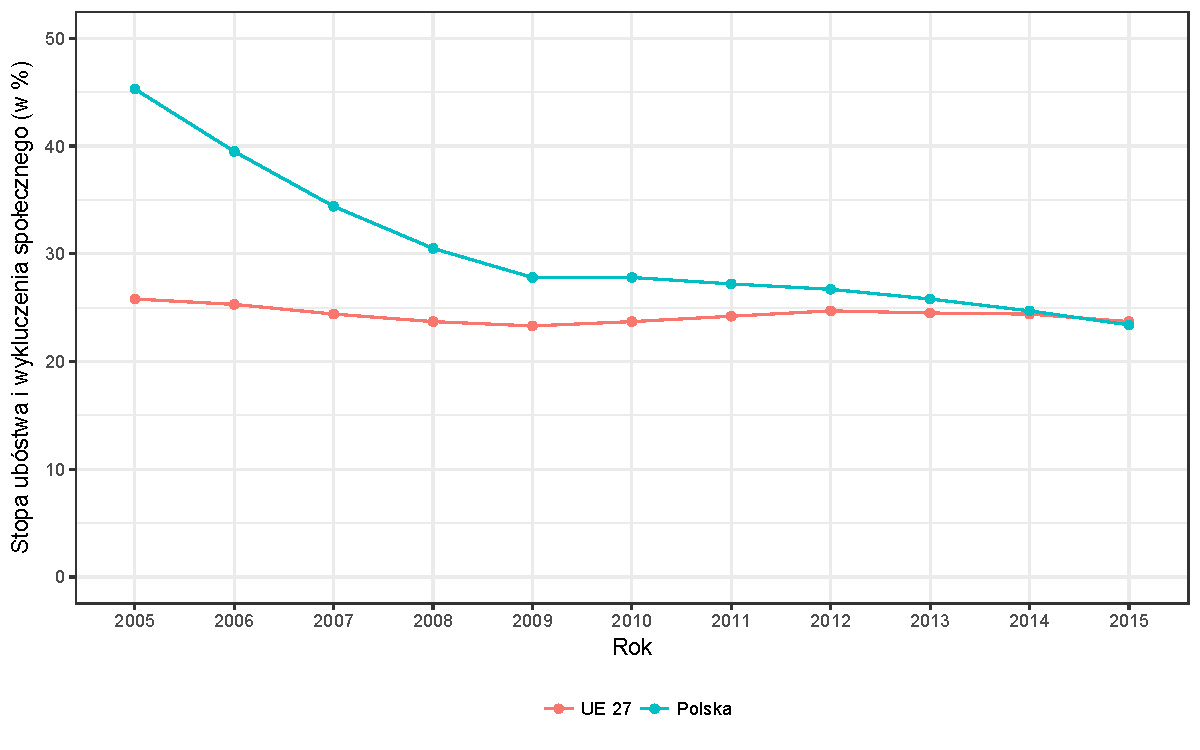
\includegraphics[width=\textwidth]{01_wykresy/europa2020-1.pdf}
\caption{Stopa ubóstwa i wykluczenia społecznego w latach 2005--2015 w Unii Europejskiej oraz Polsce}
\small{Źródło: opracowanie własne na podstawie danych Eurostatu.}
\label{fig:europa2020}
\end{figure}

W 2005 roku w Polsce prawie połowa populacji była zagrożona ubóstwem lub wykluczeniem społecznym. Od tego czasu wskaźnik ten systematycznie maleje i w roku 2015 kształtował się na poziomie nieznacznie niższym od wartości oszacowanej dla Unii Europejskiej. Niemniej oznacza to, że w Polsce żyje około 8,7 mln osób dotkniętych ubóstwem i wykluczeniem społecznym. Z kolei w UE wartość wskaźnika oscyluje w okolicy 25\% i utrzymuje się na stałym poziomie, co oznaczało około 117,6 mln osób żyjących w ubóstwie w 2015 roku. Biorąc pod uwagę fakt, że w 2010 roku w 27 krajach Unii Europejskiej żyło 116,82 mln ludzi ubogich, cel postawiony w Strategii Europa 2020 prawdopodobnie nie zostanie osiągnięty. O ile w Polsce ubóstwo maleje, trend wzrostowy odnotowywany jest w Estonii, Grecji, Hiszpanii, Portugalii, Słowenii czy Szwecji.

Narzędziem realizacji celów strategii Europa 2020 w Polsce jest Krajowy Program Reform powołany do życia w 2011 roku \citep{mr2011}. Zgodnie z tym dokumentem europejski cel strategii określony jako ``Zmniejszenie liczby osób zagrożonych ubóstwem lub wykluczeniem społecznym o 20 mln'' został dostosowany do polskiej sytuacji jako obniżenie o 1,5 mln liczby osób zagrożonych ubóstwem i/lub deprywacją materialną i/lub żyjących w gospodarstwach domowych bez osób pracujących lub o niskiej intensywności pracy. Działania w zakresie przeciwdziałaniu wykluczeniu społecznemu skupiają się przede wszystkim na zwiększaniu szans na zatrudnienie osób młodych, o niskim poziomie wykształcenia, złym stanie zdrowia, niepełnosprawnych czy imigrantów. Większość zadań została przekazana do realizacji Ministerstwu Pracy i Polityki Społecznej\footnote{Od 16 listopada 2015 roku Ministerstwo Rodziny, Pracy i Polityki Społecznej.}.

Raport z roku 2015 dotyczący postępów w zakresie przeciwdziałania ubóstwu zawiera informacje o zmniejszaniu się wskaźników ubóstwa i wykluczenia społecznego oraz przegląd podjętych działań. Wśród nich można wymienić m.in. nowelizację ustawy o promocji zatrudnienia i instytucjach rynku pracy, prowadzenie prac nad założeniami do ustawy o zmianie ustawy o pomocy społecznej czy wprowadzenie ustawy o Karcie Dużej Rodziny. Został także utworzony nowy program rozwoju pt. ``Krajowy Program Przeciwdziałaniu Ubóstwu i Wykluczeniu Społecznemu 2020. Nowy wymiar aktywnej integracji'' \citep{mr2015}.

Należy podkreślić, że działania prowadzone w ramach przedstaw wyżej przedsięwzięć nie koncentrują się przeciwdziałaniu ubóstwu poprzez świadczenia społeczne. Pomoc społeczna jest traktowana jako podstawowe narzędzie w ograniczaniu biedy, ale w rzeczywistości zwykle tylko zwiększa dochód obecny \citep{barr2016}. 

\subsection{Projekty badawcze}

Zjawisko ubóstwa jest także tematem badań wielu zespołów naukowców, których celem jest wypracowanie nowych metod analizy oraz nowych wskaźników mierzących niedostatek. W niniejszej części pracy zostaną zaprezentowane najważniejsze z nich.

\subsubsection*{SAIPE --- Small Area Income and Poverty Estimates}

Celem programu SAIPE jest dostarczenie oszacowań wskaźników ubóstwa dla szczegółowych przekrojów terytorialnych w Stanach Zjednoczonych. Docelowym poziomem estymacji są stany, hrabstwa oraz okręgi szkolne. Wykorzystując dane pochodzące z rejestrów administracyjnych, spisów powszechnych oraz badania reprezentacyjnego American Community Survey, amerykańskie biuro spisowe rokrocznie dostarcza rzetelnych oszacowań dla nieplanowanych domen. Wśród cech, które są szacowane znalazły się m.in. liczba osób dotkniętych ubóstwem, liczba dzieci życzących w ubóstwie w różnych grupach wieku oraz mediana dochodów gospodarstw domowych. Oszacowanie wartości tych zmiennych jest możliwe poprzez zastosowanie modelu Faya-Herriota oraz podejścia bayesowskiego. Metodologia programu jest nieustannie doskonalona w celu dostarczenia precyzyjnych szacunków ubóstwa. Na ich postawie lokalne władze zarządzają federalnymi programami pomocowymi \citep{saipe}.

\subsubsection*{AMELI --- Advanced Methodology for European Laeken Indicators}

Celem projektu realizowanego w latach 2008--2011 przez 10 instytucji europejskich był rozwój metodyki szacowania tzw. wskaźników lejkenowskich. Projekt składał się z 10 pakietów roboczych. Wykonawcy projektu w pierwszej kolejności określili aktualny stan wiedzy dotyczący wskaźników lejkenowskich. W przeglądzie literatury wskazują wykorzystanie analizowanych wskaźników w~różnych metodach, badaniach oraz publikacjach. Kolejny etap projektu dotyczył metod estymacji wskaźników za pomocą metod klasycznych oraz statystyki małych obszarów. W dalszej kolejności autorzy skupili się na metodach szacowania wariancji oraz estymacji odpornej. Kolejne pakiety robocze zawierały już wyniki przeprowadzonych obliczeń, których podstawę stanowiło badanie EU-SILC. Uzupełnienie raportów stanowi osiem pakietów napisanych w języku R \citep{ameli}

\subsubsection*{SAMPLE --- Small Area Methods for Poverty and Living Condition Estimates}

Podobnie jak projekt AMELI projekt SAMPLE był realizowany w latach 2008--2011 i także był finansowany w ramach siódmego programu ramowego w zakresie badań naukowych (7PR). W tej inicjatywie brały udział dwie polskie instytucje: Szkoła Główna Handlowa oraz Główny Urząd Statystyczny. Projektowi realizowanemu przez międzynarodowe konsorcjum przewodniczyła profesor Monica Pratesi (Uniwersytet w Pizie). W projekcie zaplanowano 6 pakietów roboczych. Celem pierwszego z nich był przegląd literatury dotyczącej wskaźników ubóstwa oraz weryfikacja podejść stosowanych w estymacji ubóstwa. Zaproponowano nowe podejście do estymacji ubóstwa bazujące na zbiorach rozmytych. Drugi pakiet roboczy zawierał opis istniejącej oraz nowej metodyki w zakresie estymacji ubóstwa dla nieplanowanych domen. Wszystkie metody zostały oprogramowane w języku R. Wypracowaną metodykę poparto przykładami na rzeczywistych danych pochodzących z badań EU-SILC przeprowadzonych we Włoszech oraz Hiszpanii. Następnie zespół projektowy zbadał dostępność danych dotyczących warunków życia oraz polityki społecznej na poziomie lokalnym. Celem czwartego pakietu roboczego było utworzenie oprogramowania umożliwiającego niewykwalifikowanym użytkownikom korzystanie z wypracowanych metod oraz wyników. Dwa ostatnie pakiety robocze dotyczyły spraw organizacyjnych \citep{sample}. 

\vspace{1em}

\noindent W Polsce także zrealizowano kilka projektów, których celem była estymacja wskaźników ubóstwa dla małych domen.

\subsubsection*{Wykluczenie i integracja społeczna w Polsce}

W projekcie prowadzonym we współpracy polskich naukowców z ośrodkami w Niemczech, Słowacji oraz Włoszech dokonano analizy wskaźnikowej wykluczenia społecznego. Jednym z elementów tej analizy było wykorzystanie metod statystyki małych obszarów do estymacji wybranych wskaźników na poziomie powiatów. W tym celu wykorzystano klasyczny model Faya-Herriota \citep{fh1979} oraz dane jednostkowe pochodzące z Badania Budżetów Gospodarstw Domowych. Szacowano dochód ekwiwalentny oraz dochód \textit{per capita}, a także logarytmy tych cech. Ponadto obliczono kompozytowy wskaźnik ubóstwa będący średnią ważoną wartości stóp ubóstwa dla granic określonych na poziomie 50\%, 60\% oraz 70\% mediany dochodów. W zastosowanych modelach znalazły się takie zmienne niezależne jak: odsetek osób z wykształceniem wyższym wśród osób w wieku 15--64 lata, odsetek bezrobotnych długookresowo (powyżej 1 roku) wśród bezrobotnych w wieku 15--64 lata, przeciętna liczba osób na 1 pokój (logarytm naturalny), odsetek ludności w~mieszkaniach zamieszkanych stale bez wodociągu czy odsetek osób w rodzinach z co najmniej 3~dzieci w wieku do lat 24 pozostających na utrzymaniu \citep{wykluczenie2006}.

\subsubsection*{Mapy ubóstwa na poziomie podregionów w Polsce z wykorzystaniem estymacji pośredniej}

Projekt realizowany w latach 2013--2014 przy udziale Banku Światowego, Głównego Urzędu Statystycznego oraz Urzędu Statystycznego w Poznaniu miał na celu oszacowanie wartości stopy ubóstwa w przekroju podregionów w Polsce. Na podstawie danych jednostkowych z badania EU-SILC 2011 oszacowano stopę ubóstwa z wykorzystaniem estymatora bezpośredniego. Wartości te stanowiły zmienną zależną w zastosowanym później modelu Faya-Herriota. Jako zmienne pomocnicze wykorzystano wskaźniki pochodzące z Narodowego Spisu Powszechnego Ludności i~Mieszkań 2011 oraz Banku Danych Lokalnych. W modelu znalazły się takie zmienne jak odsetek liczby osób samotnych powyżej 25 roku życia, liczba pokoi przypadająca na członka gospodarstwa domowego, odsetek gospodarstw domowych posiadających łazienkę, odsetek gospodarstw domowych z~dwiema osobami powyżej 25 roku życia z wykształceniem co najwyżej zawodowym, gęstość zaludnienia oraz stosunek liczby osób wymeldowanych do liczby zameldowanych na pobyt stały w~podregionie. W rezultacie uzyskano oszacowania pośrednie stopy ubóstwa na poziomie podregionów, charakteryzujące się lepszą precyzją aniżeli oszacowania otrzymane na podstawie estymatora bezpośredniego. Otrzymane wyniki wskazały na występowanie terytorialnego zróżnicowania ubóstwa --- wschodnia część kraju cechuje się wyższym odsetkiem osób ubogich w~porównaniu do części centralnej i zachodniej \citep{mapowanie2014}.

\subsubsection*{Pomiar ubóstwa na poziomie powiatów}

Praca badawcza była realizowana w latach 2013--2015 w ramach projektu o nazwie \textit{Statystyka dla polityki spójności} finansowanego ze środków Europejskiego Funduszu Rozwoju Regionalnego w ramach Programu Operacyjnego Pomoc Techniczna 2007--2013  --- oś priorytetowa 3  „Wsparcie realizacji operacji funduszy strukturalnych”, działanie 3.1 „Wsparcie instytucji zaangażowanych w realizację NSRO”. Celem projektu było oszacowanie stopy ubóstwa na poziomie powiatów w~latach 2005, 2008 oraz 2011. Projekt był podzielony na dwie części. W pierwszej, mającej charakter teoretyczny, zespół badawczy dokonał przeglądu literatury, wskazał możliwe źródła danych w~estymacji poziomu ubóstwa, przeprowadzono także kwerendę dotyczącą najistotniejszych zmiennych pomocniczych w estymacji stopy ubóstwa. W raporcie zawarto przegląd najważniejszych metod z zakresu statystyki małych obszarów oraz zaproponowano kilka narzędzi informatycznych użytecznych w estymacji ubóstwa. W drugim etapie przedstawiono teoretyczne aspekty pomiaru ubóstwa oraz uzupełniono opis zastosowanych estymatorów. Estymację stopy ubóstwa poprzedzono analizą taksonomiczną. Oszacowania stopy ubóstwa dla lat 2005, 2008 oraz 2011 na poziomie powiatów uzyskano wykorzystując jednostkowe dane z badania EU-SILC oraz wskaźniki z Banku Danych Lokalnych. Zastosowano estymatory uwzględniające korelacje w czasie oraz przestrzeni \citep{raoyu1994,faydiallo2012}. Ponadto dla roku 2011, z racji dostępności danych z Narodowego Spisu Powszechnego Ludności i Mieszkań 2011 oszacowano wartości stopy ubóstwa z wykorzystaniem estymatora EB \citep{ebp2010}. Na podstawie przeprowadzonych prac zespół badawczy zarekomendował dalsze rozwijanie metodologii szacowania ubóstwa na niskich poziomach agregacji przestrzennej w Polsce \citep{pomiar2015}.

\section{Ubóstwo w Polsce}

Ta część rozdziału poświęcona jest zjawisku ubóstwa wyłącznie w odniesieniu do Polski. W pierwszej kolejności przeanalizowano obowiązujące w naszym kraju kryteria ubóstwa w ujęciu czasowym. Na ich postawie obliczono wskaźnik zasięgu ubóstwa. W dalszej części omówiono przestrzenny wymiar ubóstwa w Polsce z uwzględnieniem podziału NUTS 2. Wizualizacje wartości stopy ubóstwa zaprezentowano w postaci kartogramów.

\subsection{Czasowy wymiar ubóstwa}\label{pr:czasowy-wymiar-ubostwa}

W Polsce można wyróżnić pięć kryteriów oceny ubóstwa: minimum socjalne, minimum egzystencji, ustawową granicę ubóstwa oraz relatywną granicę ubóstwa obliczaną na podstawie dwóch badań reprezentacyjnych (BBGD i EU-SILC). W tej części pracy przedstawiono porównanie wartości tych kryteriów oraz otrzymanych na ich podstawie wartości zasięgu ubóstwa wykorzystując dostępne dane z lat 2005--2015. Na rysunku \ref{fig:gr_1os} przedstawiono wyznaczone granice ubóstwa dla gospodarstwa jednoosobowego.

\begin{figure}[ht]
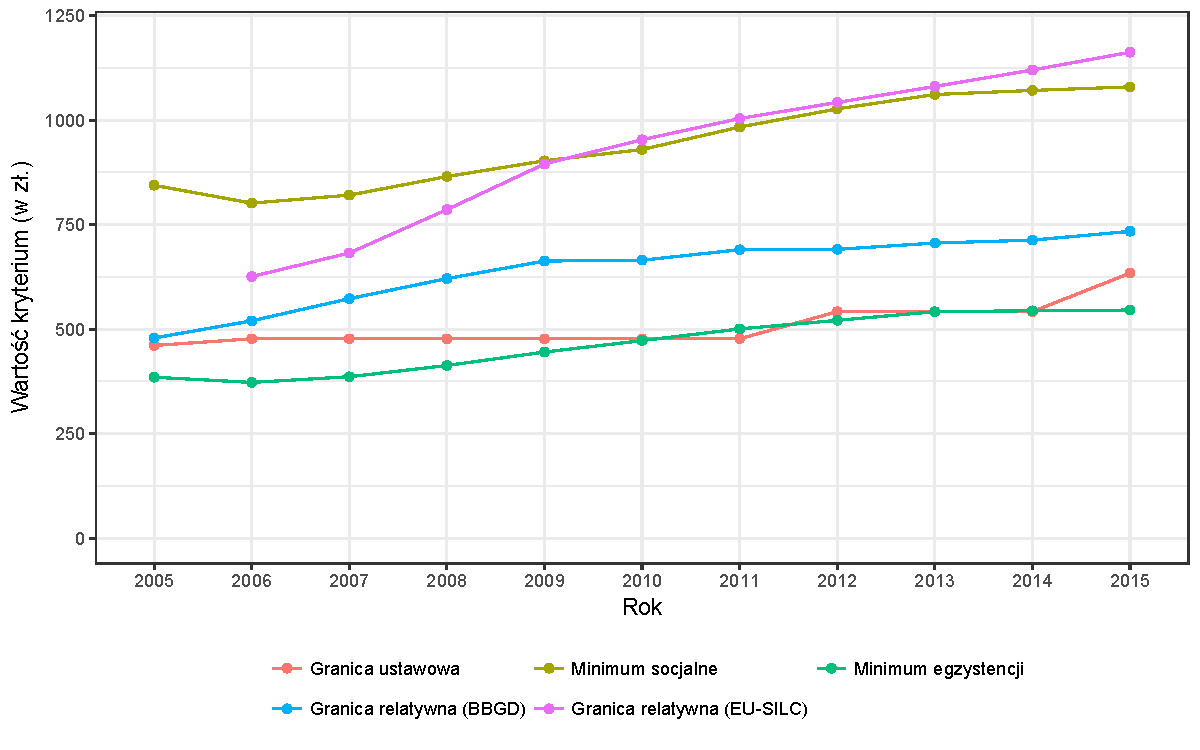
\includegraphics[width=\textwidth]{01_wykresy/gr_1os-1.pdf}
\caption{Granice ubóstwa dla gospodarstwa jednoosobowego w latach 2005--2015 w Polsce}
\small{Źródło: opracowanie własne na podstawie danych GUS, IPiSS oraz MRPiPS.}
\label{fig:gr_1os}
\end{figure}

Analizując wartości przedstawione na rysunku \ref{fig:gr_1os} należy zwrócić uwagę na kilka aspektów. Granica ubóstwa ustawowego oraz relatywnego obliczona na podstawie EU-SILC w odróżnieniu od pozostałych wartości opiera się na dochodach, a nie wydatkach. Ponadto wartości dla tej drugiej granicy dostępne są dopiero od roku 2006, ponieważ dopiero od tego roku wtedy GUS zaczął realizować badanie EU-SILC. Interpretacja wartości przestawionych na rysunku pozwala na zaobserwowanie pewnych zależności. Widoczne jest podobieństwo pomiędzy poziomem granicy ubóstwa ustawowego oraz ubóstwa skrajnego. Podobnie w przypadku wartości minimum socjalnego oraz relatywnej granicy ubóstwa dla EU-SILC --- od roku 2009 obie wartości kształtują się na podobnym poziomie. Natomiast granica ubóstwa relatywnego wyznaczona jako 50\% średniej wydatków jest wyższa od minimum egzystencji i granicy ubóstwa ustawowego, ale niższa od minimum socjalnego i granicy ubóstwa relatywnego wyznaczonego jako 60\% mediany dochodu.

Rysunek \ref{fig:gr_4os} przedstawia granice ubóstwa dla gospodarstwa 4-osobowego.

\begin{figure}[ht]
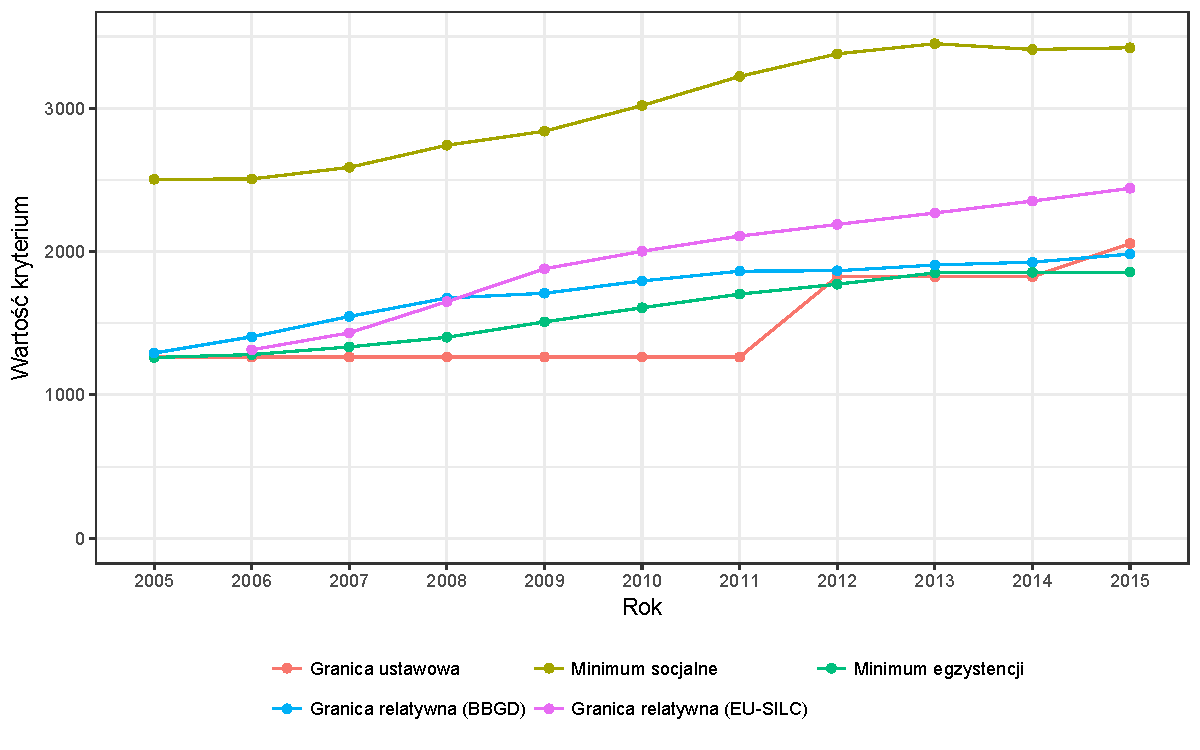
\includegraphics[width=\textwidth]{01_wykresy/gr_4os-1.pdf}
\caption{Granice ubóstwa dla gospodarstwa 4-osobowego w latach 2005--2015 w Polsce}
\small{Źródło: opracowanie własne na podstawie danych GUS, IPiSS oraz MRPiPS.}
\label{fig:gr_4os}
\end{figure}

W tym przypadku widoczny jest podział analizowanych granic ubóstwa na dwie grupy o~podobnych wartościach. Najniższymi wartościami cechują się granice ubóstwa ustawowego oraz skrajnego, które w poszczególnych latach się przecinają. Wyższymi wartościami od granic już wymienionych cechują granice ubóstwa relatywnego wyznaczone na podstawie BBGD i EU-SILC. Mimo znaczących różnic metodycznych obie z nich kształtują się na podobnym poziomie. Wyraźnie wyższa jest z kolei wartość minimum socjalnego.

Na rysunku \ref{fig:gr_stopa_ub} przedstawiono wartości stopy ubóstwa biorąc pod uwagę wcześniej scharakteryzowane granice ubóstwa.

\begin{figure}[ht]
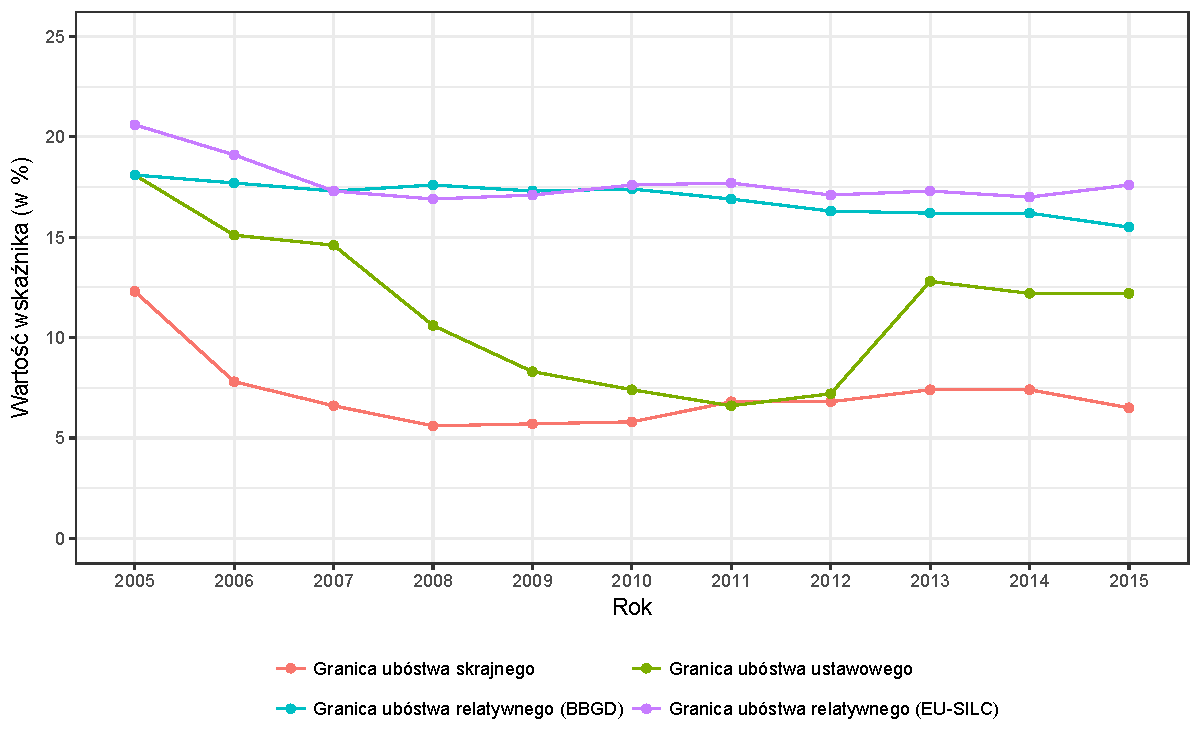
\includegraphics[width=\textwidth]{01_wykresy/gr_stopa_ub-1.pdf}
\caption{Stopa ubóstwa wyznaczona na podstawie różnych granic ubóstwa w latach 2005--2015 w Polsce}
\small{Źródło: opracowanie własne na podstawie danych GUS, IPiSS oraz MRPiPS.}
\label{fig:gr_stopa_ub}
\end{figure}

Ubóstwo skrajne systematycznie malało od roku 2005 do 2008. Przez trzy lata wskaźnik ten kształtował się na stałym poziomie, po czym nastąpił wzrost do poziomu 7,4\% w 2014 roku. Podobny trend można było obserwować w przypadku granicy ubóstwa ustawowego - od roku 2005 do 2011 następował spadek odsetka osób w gospodarstwach domowych zagrożonych ubóstwem ustawowym. W 2011 roku doszło do sytuacji, w której osób dotkniętych skrajnym ubóstwem było więcej od osób uprawnionych do korzystania ze świadczeń pomocy społecznej. W kolejnych latach obserwowany jest wzrost stopy ubóstwa do poziomu 12,2\% w roku 2014. Z kolei zasięg ubóstwa relatywnego jest szacowany w Polsce w oparciu o dwa źródła: Badanie Budżetów Gospodarstw Domowych (BBGD) oraz Europejskie Badanie Dochodów i Warunków Życia (EU-SILC). W pierwszym z nich jako granicę ubóstwa przyjmuje się 50\% średnich wydatków gospodarstw domowych, natomiast w drugim 60\% mediany dochodów. W obu badaniach stosowana jest zmodyfikowana skala ekwiwalentności OECD. Mimo istotnych różnic w zastosowanej metodologii otrzymane wartości zasięgu ubóstwa są do siebie bardzo zbliżone w kolejnych latach. Trend w latach 2005--2015 jest malejący, a największą różnicę odnotowano w roku 2005 (2,5 p.p.). Z kolei w 2007 roku oba oszacowania były identyczne.

Na rysunku \ref{fig:stopa_gleb} zestawiono wartości wskaźników ubóstwa w latach 2005-2015 obliczonych na podstawie badania EU-SILC.

\begin{figure}[ht]
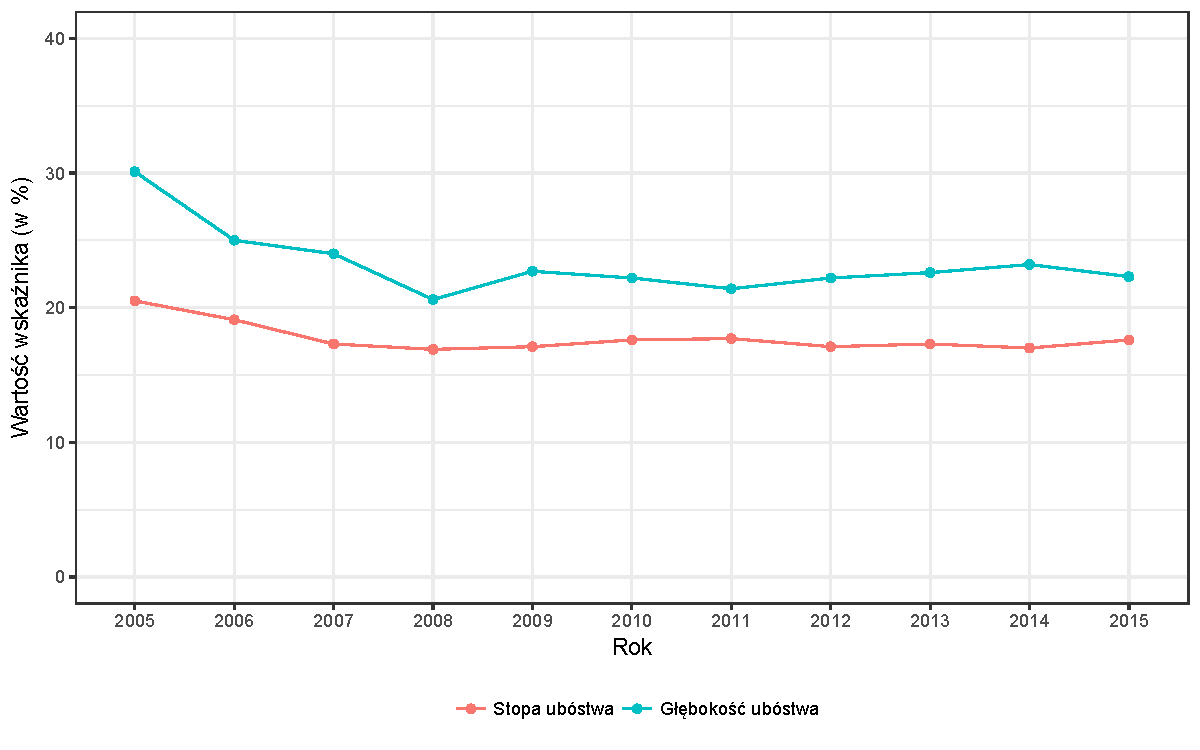
\includegraphics[width=\textwidth]{01_wykresy/stopa_gleb-1.pdf}
\caption{Stopa oraz głębokość ubóstwa w latach 2005--2015 w Polsce}
\small{Źródło: opracowanie własne na podstawie danych Eurostatu.}
\label{fig:stopa_gleb}
\end{figure}

W latach 2005-2015 wartości stopy ubóstwa charakteryzowały się tendencją malejącą - z 20,5\% do 17,0\%. Oznacza to, że w 2015 roku poniżej granicy ubóstwa żyło w Polsce około 6,5 mln osób. Wskaźnik głębokości ubóstwa cechował się występowaniem większych fluktuacji od pozostałych mierników. Wartości luki dochodowej od roku 2005 do roku 2008 systematycznie malały, po czym w 2009 nastąpił wzrost do poziomu 22,7\%. Następnie ponownie wartości głębokości ubóstwa miały tendencję spadkową, aż do roku 2011, kiedy trend ponownie zmienił kierunek. W roku 2014 luka dochowa wynosiła 22,3\%, co oznacza, że dochody osób ubogich były przeciętnie niższe od granicy ubóstwa o 22,3\%. Rosnąca w czasie różnica pomiędzy stopą i głębokością ubóstwa może doprowadzić do tego, że pomimo stałego odsetka osób ubogich, będą one miały coraz niższe dochody.

\subsection{Przestrzenne zróżnicowanie ubóstwa}

Zgodnie z Klasyfikacją Jednostek Terytorialnych do Celów Statystycznych --- NUTS, w Polsce wyróżnia się pięć poziomów terytorialnych. Poziom regionalny obejmuje trzy z nich: makroregiony (NUTS 1), województwa (NUTS 2) i podregiony (NUTS 3). Natomiast na poziomie lokalnym są powiaty (NUTS 4) oraz gminy (NUTS 5). Zgodnie z nomenklaturą UE jednostki lokalne określane są również jako LAU 1 oraz LAU 2 \citep{eurostat2011}. Według stanu na 1 stycznia 2015 r. w~Polsce było 6 jednostek NUTS 1, 16 jednostek NUTS 2, 72 jednostki NUTS 3, 380 jednostek NUTS 4~oraz 3737 jednostek NUTS 5. Wśród ważniejszych modyfikacji klasyfikacji NUTS należy wymienić zmianę z 1 stycznia 2013 r. polegającą na dodaniu jednej jednostki na poziomie NUTS 4 --- miasta na prawach powiatu Wałbrzych oraz zwiększenie liczby podregionów z 66 do 72 w~dniu 1~stycznia 2015 roku.

Dane dotyczące stopy ubóstwa w Polsce publikowane są przez GUS na podstawie BBGD i~EU-SILC. W przypadku pierwszego badania, informacje dostępne są na poziomie całego kraju oraz województw (NUTS 2). Z kolei na podstawie badania EU-SILC w latach 2005--2011 stopa ubóstwa była publikowana na poziomie całego kraju, makroregionów (NUTS 1) oraz województw (NUTS 2), natomiast od roku 2012 zredukowano dostępność szacunków do poziomu kraju oraz makroregionów (NUTS 2).

Na rysunku \ref{fig:arpr_nts2_bbgd_silc_2011} przedstawiono zasięg ubóstwa relatywnego w 2011 roku w województwach Polski według dwóch badań --- BBGD i EU-SILC.

\begin{figure}[ht]
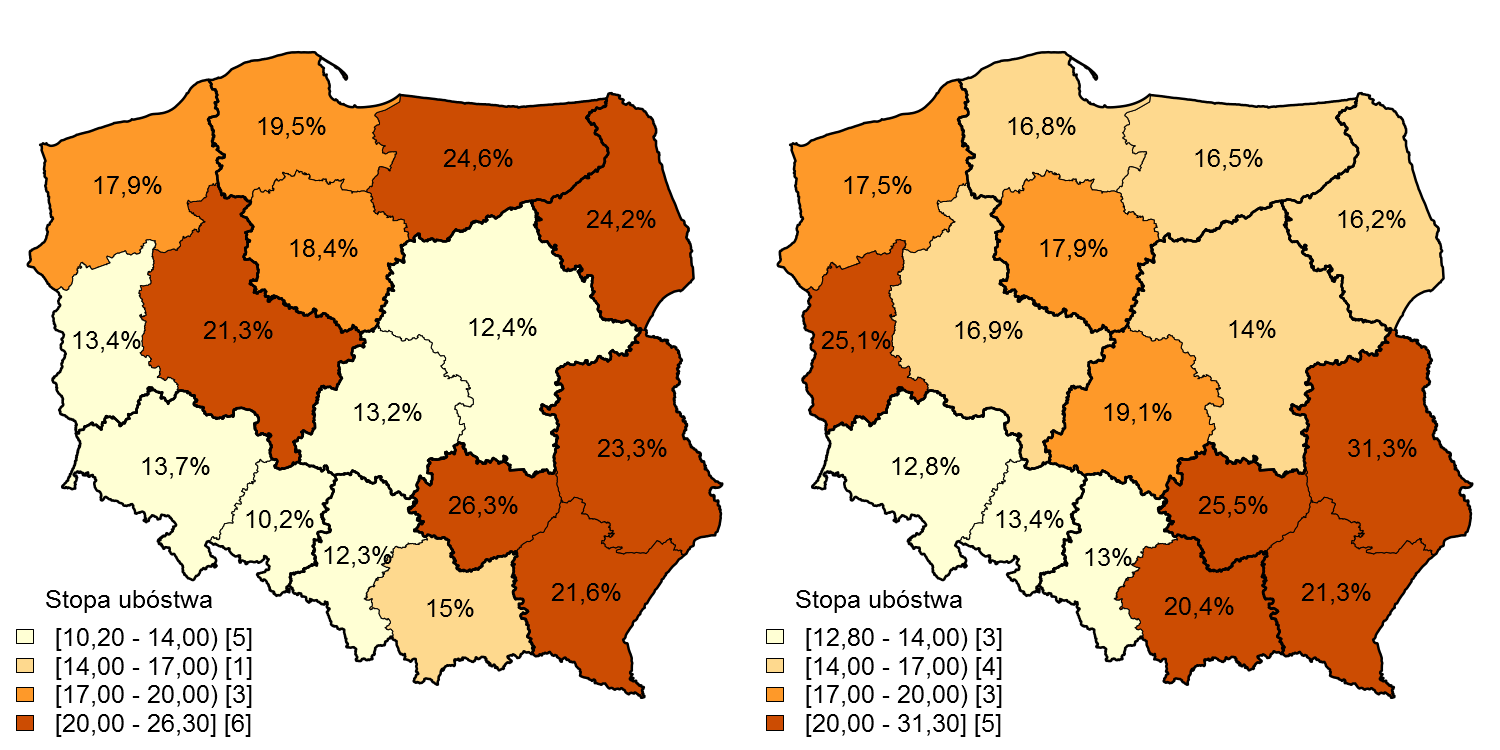
\includegraphics[width=\textwidth]{01_wykresy/arpr_nts2_bbgd_silc_2011.png}
\caption{Stopa ubóstwa na podstawie badania BBGD (po lewej stronie) oraz na podstawie badania EU-SILC (po prawej stronie) w roku 2011 w przekroju województw}
\small{Źródło: opracowanie własne na podstawie BBGD 2011 i EU-SILC 2011.}
\label{fig:arpr_nts2_bbgd_silc_2011}
\end{figure}

Dane zawarte na rysunku \ref{fig:gr_stopa_ub} wskazywały, że pomimo zastosowania różnych kryteriów ubóstwa, wartości stopy ubóstwa nie różniły się znacząco pomiędzy badaniami BBGD oraz EU-SILC. Niemniej analiza tego wskaźnika w przekroju województw uwydatnia istniejące różnice. Największe różnice występują w województwach: lubuskim, łódzkim, małopolskim, podlaskim, warmińsko-mazurskim oraz wielkopolskim. Wspólny dla obu badań jest obraz niskiego ubóstwa na terenach Śląska oraz złej sytuacji gospodarstw w południowo-wschodniej części Polski. Podobne wartości, przeciętnego poziomu ubóstwa, można z kolei zaobserwować w północno-zachodniej części kraju.

Informacje o głębokości ubóstwa nie są publikowane w ujęciu przestrzennym.

\section{Podsumowanie}

W rozdziale przedstawiono definicję ubóstwa oraz sposoby pomiaru tego zjawiska. Wskazano powody, dla których analizy niedostatku nie należy ograniczać wyłącznie do jednego wskaźnika --- stopy ubóstwa. Konieczne jest także wyznaczenie głębokości ubóstwa. Na podstawie literatury przedmiotu oraz badań empirycznych scharakteryzowano główne determinanty ubóstwa. Zaprezentowano także działania pokazujące, że problem ubóstwa nie jest bagatelizowany przez instytucje krajowe oraz międzynarodowe. W ostatnich latach zrealizowano wiele projektów badawczych mających na celu wypracowanie nowych metod analizy ubóstwa oraz estymacji wskaźników niedostatku w szczegółowych przekrojach terytorialnych. 

Na podstawie dostępnych danych pochodzących z badań reprezentacyjnych GUS oraz obliczeń Instytutu Pracy i Spraw Socjalnych, przeanalizowano stosowane w Polsce kryteria ubóstwa w ujęciu czasowym. Biorąc pod uwagę lata 2005--2015 zestawiono ze sobą granice ubóstwa wyznaczane według różnych metod, a następnie na tej podstawie obliczono zasięg ubóstwa. Wykazano wysoką korelację pomiędzy wartościami stopy ubóstwa szacowanej na podstawie dwóch badań reprezentacyjnych --- Badania Budżetów Gospodarstw Domowych oraz Europejskiego Badania Dochodów i Warunków Życia.

Przegląd dostępnych danych w ujęciu przestrzennym pozwolił na identyfikację obszarów mniej i bardziej zagrożonych ubóstwem. Była to jednak analiza na bardzo wysokim stopniu ogólności --- województw, ponieważ na tym poziomie były publikowane wartości stopy ubóstwa. Na tej podstawie nie można było przeprowadzić kompleksowej analizy ubóstwa, ponieważ w tym celu należałoby znać przestrzenny rozkład także głębokości ubóstwa. Ten wskaźnik nie jest publikowany w żadnych przekrojach terytorialnych. 

\chapter{Źródła danych na temat ubóstwa}
\section{Wprowadzenie}

Niniejszy rozdział zawiera przegląd źródeł danych mogących służyć zarówno jako źródła zmiennych zależnych, jak i \textit{zmiennych pomocniczych} w estymacji pośredniej. Scharakteryzowano w nim w pierwszej kolejności badania reprezentacyjne będące podstawą publicznej informacji na temat dochodów ludności Polski. Następnie, uwzględniając przede wszystkim cel pracy, Przedstawiono spisy ludności, które stanowią cenne i bogate źródło \textit{zmiennych pomocniczych} dostępnych na niskich poziomach agregacji przestrzennej. W rozdziale znalazły się także informacje na temat rejestrów administracyjnych zawierających dane dotyczące ubóstwa i zjawisk pokrewnych. W ostatniej, czwartej części rozdziału nawiązano do nowych i coraz częściej wykorzystywanych w analizach zasobów danych określanych mianem Big Data. W dobie powszechnego dostępu do Internetu uwzględnienie możliwości pozyskania danych do estymacji pośredniej z innych, niestatystycznych źródeł staje się bowiem jednym z obowiązkowych etapów badania.

\section{Badania reprezentacyjne}

Podstawowym źródłem danych o warunkach życia ludności w Polsce są badania reprezentacyjne prowadzone przez Główny Urząd Statystyczny. Wśród nich najpoważniejszą rolę odgrywają: Badanie Budżetów Gospodarstw Domowych (BBGD) oraz Europejskie Badanie Dochodów i Warunków Życia (EU-SILC). Od roku 2011 w cyklu czteroletnim realizowane jest także nowe badanie GUS --- Badanie Spójności Społecznej (BSS). Ponadto należy także wspomnieć o przekrojowym badaniu Diagnoza Społeczna (DS) prowadzonym przez Radę Monitoringu Społecznego. W kolejnych podrozdziałach badania te zostaną szerzej scharakteryzowane.

\subsection{Badanie Budżetów Gospodarstw Domowych}

Badanie Budżetów Gospodarstw Domowych (BBGD) jest podstawowym źródłem o przychodach, rozchodach, spożyciu ilościowym żywności oraz innych aspektów warunków życia ludności. Dane pochodzące z badania wykorzystywane są m.in. do analizy poziomu życia gospodarstw domowych, obliczania wskaźników cen towarów i usług, określenia poziomu minimalnego wynagrodzenia oraz badania ubóstwa. Schemat zgodnie z którym obecnie realizowane jest Badanie Budżetów Gospodarstw Domowych obowiązuje od 1992 roku. Co miesiąc losowana jest próba składająca się z 3132 mieszkań. Badaniu podlegają wszystkie gospodarstwa domowe zamieszkujące wylosowane mieszkanie. W przypadku odmowy udziału w badaniu, gospodarstwo jest zastępowane przez jednostkę pochodzącą z tzw. próby rezerwowej. Rokrocznie w BBGD bierze udział około 37 tys. gospodarstw.

Mieszkania do badania losowane są na podstawie dwustopniowego schematu losowania przy wykorzystaniu operatu uwzględniającego podział terytorialny kraju (TERYT). W badaniu stosuje się model rotacji całkowitej z miesięcznym okresem wymiany próby. Oznacza to, że w każdym miesiącu badane są inne jednostki. Gospodarstwa domowe uczestniczące w badaniu są zobowiązane do rejestrowania swoich przychodów i rozchodów w tzw. książeczkach budżetowych przez cały miesiąc \citep{bbgd_met2011}.

Wyniki badania publikowane są w przekroju grup społeczno-ekonomicznych, według wielkości gospodarstwa domowego, miejsca zamieszkania (miasto/wieś), według typu biologicznego gospodarstwa domowego oraz według podstawowych grup potrzeb i asortymentów towarów. Wybrane statystyki takie jak wskaźnik miesięcznych dochodów rozporządzalnych, wskaźnik przeciętnych miesięcznych wydatków na 1 osobę czy wyposażenie w wybrane dobra trwałego użytkowania przedstawiane są w przekroju województw \citep{bbgd2016}. BBGD stanowi podstawę do opracowania publikacji GUS pt. ,,Ubóstwo w Polsce'' wydawanej z częstotliwością roczną \citep{ubostwo-gus2015}.

Koszt przeprowadzenia badania w 2016 roku według informacji zawartych w Programie Badań Statystycznych Statystyki Publicznej wyniósł 26 800 300 zł \citep{pbs2015}.

\subsection{Europejskie Badanie Dochodów i Warunków Życia}

Celem Europejskiego Badania Dochodów i Warunków Życia (EU-SILC) jest dostarczenie porównywalnych danych na temat osób i gospodarstw domowych dla krajów Unii Europejskiej. Pierwszy raz zostało ono przeprowadzone w 2003 roku, a dwa lata później wdrożono je w 25 krajach Unii Europejskiej. Badanie EU-SILC stanowi podstawowe źródło danych na temat dochodów, ubóstwa i wykluczenia społecznego. Otrzymane wyniki umożliwiają monitorowanie skutków działań podejmowanych w ramach programów mających na celu ograniczanie ubóstwa takich jak np. \textit{Europa 2020}. 

EU-SILC, podobnie jak Badanie Budżetów Gospodarstw Domowych, bazuje na dwustopniowym schemacie losowania próby. W pierwszym roku badania wylosowano około 24 tys. mieszkań. Następnie, wylosowane mieszkania podzielono na 4 rozłączne i równoliczne podpróby. Od 2006 roku jedna z podprób jest wykluczana, a na jej miejsce losuje się nową podpróbę. W badaniu EU-SILC próba rezerwowa nie jest dobierana i w związku z tym w przypadku odmowy udziału, mieszkanie nie jest zastępowane innym. W znacznym stopniu niekorzystnie wpływa to na liczbę przebadanych gospodarstw. Badanie EU-SILC jest realizowane techniką bezpośredniego wywiadu z respondentem zawsze w drugim kwartale każdego roku.

Zgodnie z założeniami badania, zmienne dochodowe nie powinny zawierać braków danych. W~związku z tym, że jest to informacja wrażliwa, którą respondent dzieli się niechętnie, konieczna jest imputacja danych. W badaniu EU-SILC stosowane są cztery różne metody: hot-deck, imputacja regresyjna z losowymi resztami empirycznymi, deterministyczna imputacja regresyjna oraz imputacja dedukcyjna. Zastosowanie tych technik umożliwia uzyskanie zbioru, w którym nie występują braki danych w zakresie dochodu \citep{silc2017}.

Rezultaty badania publikowane są w przekrojach według miejsca zamieszkania (miasto/wieś), stopnia urbanizacji, regionów, cech społeczno-demograficznych respondentów, a także przedstawiane są wskaźniki dla Polski na tle Unii Europejskiej. 

Koszt przeprowadzenia badania EU-SILC w 2016 roku według informacji zawartych w Programie Badań Statystycznych Statystyki Publicznej wyniósł 4 512 600 zł \citep{pbs2015}.

\subsection{Badanie Spójności Społecznej}

Badanie Spójności Społecznej (BSS) jest badaniem o krótkiej historii. Pierwsza edycja odbyła się w 2011 roku, natomiast druga w 2015 roku. Celem badania jest kompleksowa analiza poziomu życia, ubóstwa (również w ujęciu wielowymiarowym), wykluczenia społecznego i kapitału społecznego. Nowatorski charakter badania umożliwia analizę współzależności poszczególnych zjawisk. 

W 2011 roku do badania wylosowano 26 999 mieszkań, natomiast w roku 2015 było to 27 117 mieszkań z czego 13 117 mieszkań stanowiło podpróbę panelową, a 14 000 mieszkań to były jednostki nowowylosowane. BSS jest badaniem dobrowolnym, realizowanym techniką bezpośredniego wywiadu z respondentem. W badaniu zastosowano dwustopniowy schemat losowania uwzględniając alokację próby pomiędzy województwa, w taki sposób, aby uzyskać precyzyjne wyniki na tym poziomie agregacji przestrzennej. 

Otrzymane rezultaty publikowane są w przekroju województw, grup społeczno-demograficznych oraz w podziale na miasto/wieś. Uzupełnienie tabel stanowi analiza zjawisk zakresu spójności społecznej z wykorzystaniem metod wskaźnikowych oraz regresji logistycznej \citep{jakosc-gus2013,jakosc-gus2017}. 

Koszt organizacji badania w 2011 roku wyniósł 5 434 700 zł, a w 2015 roku 6 896 460 zł ze względu na zwiększony zakres tematyczny \citep{pbs2010,pbs2014}.

\subsection{Diagnoza Społeczna}

Badanie Diagnoza Społeczna (DS) jest organizowane przez Radę Monitoringu Społeczna przy wsparciu ankieterów GUS. Jego głównym celem jest pomiar warunków życia gospodarstw domowych oraz stylu i jakości życia indywidualnych respondentów. Do tej pory odbyło się osiem edycji tego badania: w 2000, 2003, 2005, 2007, 2009, 2011, 2013 oraz 2015 roku. 

W Diagnozie Społecznej wykorzystano dwustopniowy schemat losowania próby. Co roku w~badaniu bierze udział około 12 tys. gospodarstw domowych. Autorzy wskazują, że w 2015 roku udało się przeprowadzić wywiad z 525 gospodarstwami, które znalazły się w próbie podczas pierwszej edycji badania w 2000 roku.

Wyniki badania dotyczące gospodarstw domowych publikowane są w przekroju grup społeczno-ekonomicznych, typu gospodarstwa oraz województw. Z kolei charakterystyki osób przedstawiane są w grupach tworzonych ze względu na wiek, płeć, miejsce zamieszkania, województwo, wykształcenie oraz status społeczno-zawodowy.

Badanie finansowane jest z pieniędzy prywatnych oraz publicznych. Wśród sponsorów projektu można wyróżnić m.in. Ministerstwo Pracy i Polityki Społecznej, Narodowy Bank Polski oraz PKO Bank Polski. Tym, co odróżnia Diagnozę Społeczną od badań realizowanych przez GUS jest dostępność do danych. Wyniki badania DS udostępniane są na stronie internetowej projektu w postaci jednostkowych baz danych \citep{diagnoza-panek2015}.

\section{Spisy ludności}

Najbogatszym źródłem \textit{zmiennych pomocniczych} wykorzystywanych w estymacji pośredniej są spisy powszechne. Należą do grupy badań pełnych, a więc objęta jest nimi cała populacja generalna. To z kolei oznacza, że nie są obciążone błędem losowym. Ze względu na duży koszt organizacji i przeprowadzenia realizowane są co około 10 lat.

\subsection{Narodowy Spis Powszechny Ludności i Mieszkań 2002}

Narodowy Spis Powszechny Ludności i Mieszkań 2002 (NSP 2002) czyli pierwszy spis powszechny w XXI wieku w Polsce został przeprowadzony od 21 maja do 8 czerwca 2002 roku. Równolegle odbywał się także Powszechny Spis Rolny. Spis powszechny w 2002 roku miał szczególne znaczenie, ponieważ odbył się po okresie zmian ustrojowych --- poprzedni spis pełny przeprowadzono w 1988 roku. W zakresie spisu ludności i mieszkań w 2002 znalazły się następujące obszary: geograficzna, demograficzna i społeczna charakterystyka ludności, demograficzna charakterystyka gospodarstw domowych i rodzin, niepełnosprawność, aktywność ekonomiczna oraz źródła utrzymania osób i~gospodarstw domowych. W zakresie mieszkań badano stan zasobów mieszkaniowych, wielkość mieszkań i ich wyposażenie, samodzielność zamieszkiwania oraz charakterystykę budynków. 

Dodatkowo w ramach spisu powszechnego przeprowadzono dwa badania towarzyszące: badanie dzietności kobiet oraz badanie długookresowych migracji ludności w latach 1989--2002.

Zebrane dane umożliwiły publikację informacji na temat osób aktywnych ekonomicznie według płci i wieku produkcyjnego na poziomie miejscowości statystycznych, a według poziomu wykształcenia i wieku na poziomie gmin. Natomiast zestawienie wieku, poziomu wykształcenia i statusu na rynku pracy umożliwiło publikację wyników na poziomie powiatów. W tym samym przekroju zaprezentowano także dane dotyczące osób bezrobotnych wg okresu poszukiwania pracy. Informacje dotyczące źródła utrzymania gospodarstwa domowego, typu gospodarstwa oraz liczby dzieci są dostępne na poziomie NUTS 5. Również na poziomie gmin obserwowane są statystyki ludności dotyczące wykształcenia, stanu cywilnego oraz niepełnosprawności. 

Wyniki Narodowego Spisu Powszechnego Ludności i Mieszkań 2002 zostały przedstawione w~13 publikacjach tematycznych \citep{gus2003}.

\subsection{Narodowy Spis Powszechny Ludności i Mieszkań 2011}

Narodowy Spis Powszechny Ludności i Mieszkań 2011 (NSP 2011) odbył się 9 lat po NSP 2002. W międzyczasie Polska stała się członkiem Unii Europejskiej, co spowodowało konieczność ujednolicenia systemów statystycznych do europejskich norm. Zgodnie z rozporządzeniami UE oraz ONZ, spisy powszechne powinny odbywać się na przełomie dekad w roku kończącym się cyfrą "1". Ponadto GUS został zobligowany do przekazania danych ze spisu powszechnego do Biura Statystycznego Komisji Europejskiej –-- EUROSTATu. 

Zakres tematyczny NSP 2011 obejmował te same tematy co NSP 2002, tak żeby było możliwe porównanie charakterystyk ludności na przełomie dekady. Ponadto do tematów NSP 2011 włączono dojazdy do pracy, narodowość i język, mniejszości narodowe i etniczne oraz wyznanie (przynależność do kościoła lub związku wyznaniowego).

NSP 2011 został przeprowadzony metodą mieszaną. Oznacza to, że dane na potrzeby spisu powszechnego zostały pozyskane z rejestrów administracyjnych. Każdy obywatel mógł te dane zweryfikować korzystając z tzw. samospisu internetowego. Ponadto na próbie 20\% populacji przeprowadzono badanie reprezentacyjne mające na celu dostarczenie szczegółowych charakterystyk ludności i gospodarstw domowych. 

Metodyka zastosowana w Narodowym Spisie Powszechnym Ludności i Mieszkań 2011 wymagała korekty wag przekrojowych uzyskanych dla 20\% próby, ponieważ oszacowania bezpośrednie nie były spójne z~wynikami spisu pełnego w zakresie podstawowych cech demograficznych. Wobec tego zastosowano kalibrację, która umożliwiła uzyskanie takich wartości wag, które zapewniały zgodność oszacowań w odniesieniu do płci, wieku oraz miejsca zamieszkania \citep{szymkowiak2014}.

Ze względu na inną metodę realizacji NSP 2011, nie udało się zapewnić dostępności wyników w tych samych przekrojach co w NSP 2002. Informacje na temat aktywności ekonomicznej ludności według płci są dostępne na poziomie powiatów, natomiast obserwacja tych statystyk według grup wieku jest możliwa wyłącznie w przekroju województw. Ten sam poziom agregacji przestrzennej dotyczy infomacji na temat bezrobotnych wg okresu poszukiwania pracy, biernych zawodowo wg przyczyn bierności oraz pracujących według statusu zatrudnienia. Dane na temat poziomu wykształcenia, stanu cywilnego, źródła utrzymania czy niepełnosprawności są dostępne w przekroju powiatów. Również na poziomie NUTS 4 publikowane są statystyki dotyczące gospodarstw domowych i rodzin.

Wyniki Narodowego Spisu Powszechnego Ludności i Mieszkań 2011 zostały przedstawione w~16 publikacjach tematycznych \citep{gus2012}.

\section{Rejestry administracyjne}

Zgodnie z definicją zawartą w ustawie z dnia 17 lutego 2005 roku o informatyzacji działalności podmiotów realizujących zadania publiczne, rejestrem publicznym określa się ,,rejestr, ewidencję, wykaz, listę, spis albo inną formę ewidencji, służące do realizacji zadań publicznych, prowadzone przez podmiot publiczny na podstawie odrębnych przepisów ustawowych'' (Dz. U. z 2014 r. poz. 1114, z 2016 r., poz. 352).

Rejestry administracyjne wykorzystywane są przede wszystkim w administracji rządowej. Informacje w rejestrach gromadzone są w sposób ciągły, w związku z czym mogą stanowić bardziej aktualne źródło danych o jednostkach populacji aniżeli spisy powszechne przeprowadzane co około 10 lat. Pojedyncze rejestry administracyjne zwykle mają określone przeznaczenie i nie zawierają pełnego zestawu cech opisujących obywatela.

Dane pochodzące z rejestrów administracyjnych mogą być wykorzystane w estymacji pośredniej zarówno jako zmienne pomocnicze, jak i cechy referencyjne mające na celu ocenę wiarygodności estymacji.

\subsection{Systemy Ministerstwa Finansów}

W ramach działań Ministerstwa Finansów (MF) wykorzystywanych jest 27 systemów informacyjnych. Część z nich wiąże się bezpośrednio z bieżącą obsługą działalności instytucji podległych MF, w tym organów celnych. Poniżej scharakteryzowano te systemy, które zawierają informacje istotne z punktu widzenia analizy ubóstwa. 

System \textit{Podatek Dochodowy od Osób Fizycznych (PIT)}, jak sama nazwa wskazuje, ma na celu przechowywanie zbiorczych danych na temat podatników, którzy płacą podatek dochodowy od osób fizycznych. Gromadzone są informacje o następujących cechach:

\begin{itemize}
\item kod województwa, powiatu oraz gminy,
\item NIP,
\item przychód,
\item koszty uzyskania przychodów,
\item dochód,
\item strata,
\item odliczenia od dochodu i podatku,
\item kwota należnego podatku.
\end{itemize}

Źródłem danych zasilających system PIT są roczne zeznania podatkowe.

Podobną strukturą charakteryzuje się system \textit{Ryczałt od przychodów ewidencjonowanych oraz karta podatkowa (Ryczałt)}, który zawiera informacje o płatnikach korzystających z karty podatkowej. 

Dane jednostkowe dotyczące wszystkich podatników są obsługiwane przez bazę danych POLTAX.

\subsection{Systemy Ministerstwa Pracy i Polityki Społecznej}

W gestii Ministerstwa Pracy i Polityki Społecznej leży obsługa systemów informacyjnych związanych z rejestracją bezrobotnych, niepełnosprawnych oraz korzystających z pomocy społecznej. Kompletny system składa się z kilku rejestrów oraz systemów informatycznych. 

Pierwszym z nich jest \textit{WUP-Viator}. Celem tej aplikacji jest obsługa zadań statutowych w~wojewódzkich urzędach pracy, w ramach których stanowi wsparcie procesu rejestracji i obsługi transferu osób oraz przysługujących im świadczeń pomiędzy krajami UE. Wspomaga także działania na rzecz osób poszukujących pracy oraz pracodawców. System obsługuje także szkolenia pracowników urzędów pracy. Podmiotami systemu są osoby bezrobotne, poszukujące pracy, pracodawcy oraz pracownicy wojewódzkich i powiatowych urzędów pracy. Dane w systemie są rejestrowane na bieżąco na podstawie odpowiednich dokumentów.

\textit{Elektroniczny Krajowy System Monitoringu Orzekania o Niepełnosprawności (EKSMOoN)} ma na celu przetwarzanie danych w procesie orzekania o niepełnosprawności. Działa na trzech poziomach: powiatowym, wojewódzkim i centralnym. Zawiera dane osób niepełnosprawnych oraz tych, które ubiegają się o wydanie orzeczenia o niepełnosprawności. Rejestr zawiera informacje o~następujących cechach:

\begin{itemize}
\item imię i nazwisko,
\item data i miejsce urodzenia,
\item płeć,
\item adres miejsca zameldowania i pobytu,
\item dane dokumentu tożsamości,
\item numer PESEL,
\item wykształcenie i zawód,
\item forma zatrudnienia i wymiar czasu pracy,
\item daty i rodzaje wydanych orzeczeń na temat niepełnosprawności.
\end{itemize}

Dane wprowadzane są do rejestru na bieżąco z wniosków w sprawie wydania orzeczenia o~niepełnosprawności.

Kolejnym rodzajem platformy komunikacyjnej w obszarze zabezpieczenia społecznego, umożliwiającej udostępnianie i świadczenie usług wymiany informacji, działającej przy MPiPS jest \textit{Krajowy System Monitoringu Świadczeń Rodzinnych --- ZC (KSMSR-zc)}. Celem działania tego systemu jest monitoring przyznawania i wypłaty świadczeń rodzinnych. Zawiera informacje o~zbiorowości osób otrzymujących świadczenie rodzinne wraz z danymi o składzie tych rodzin i~ich dochodach. Struktura tworzonego rejestru jest następująca:

\begin{itemize}
\item imie i nazwisko,
\item PESEL,
\item adres zamieszkania i zameldowania,
\item telefon, 
\item data urodzenia,
\item obywatelstwo,
\item stan cywilny,
\item rodzaj niepełnosprawności,
\item szkoła,
\item stopień pokrewieństwa,
\item złożone wnioski,
\item dochody (w tym dochód utracony i uzyskany),
\item opłata za placówki,
\item alimenty płacone na rzecz innych osób,
\item decyzje i wypłaty świadczeń.
\end{itemize}

Dane do zbioru centralnego przekazywane są przez gminy co kwartał.

Uzupełnieniem wyżej zaprezentowanego systemu jest \textit{Krajowy System Monitoringu Świadczeń Rodzinnych --- SPR (KSMSR-spr)}. W odróżnieniu do KSMSR-zc ten rejestr zawiera dane zagregowane o świadczeniobiorcach i rodzinach. Znaleźć w nim można między innymi informacje o~liczbie rodzin pobierających świadczenia rodzinne według liczby dzieci czy rodzaju świadczeń w podziale na grupy wieku. 

Kolejnym systemem w strukturze MPiPS jest \textit{SyriuszStd}. Ten system w odróżnieniu do \textit{WUP-Viator} wspiera powiatowe urzędy pracy w zakresie ich działań statutowych. W rejestrze znajdują się informacje o osobach bezrobotnych, poszukujących pracy oraz o pracodawcach. Wśród rejestrowanych danych można wyróżnić:

\begin{itemize}
\item dane osobowe,
\item obywatelstwo i narodowość,
\item adresy (zameldowania/zamieszkania/tymczasowy/korespondencyjny),
\item okresy zatrudnienia i urlopy wychowawcze,
\item wykształcenie, posiadane zawody, uprawnienia, umiejętności oraz znane języki obce, 
\item informacje na temat członków rodziny bezrobotnego,
\item niepełnosprawność,
\item osiągane dochody,
\item sposób wypłaty świadczenia,
\item decyzje oraz odwołania,
\item dane dotyczące wizyt w urzędzie pracy.
\end{itemize}

Dane w rejestrze rejestrowane są na bieżąco. 

Oprócz dotychczas przedstawionych systemów i rejestrów prowadzony jest także \textit{System Informatyczny Pomocy Społecznej (PS)}, którego celem jest wsparcie obsługi zadań wynikających z Ustawy o Pomocy Społecznej czyli m.in. ewidencji złożonych wniosków i wydanych decyzji, realizacji wypłaty świadczeń, obsługi zwrotów nienależnych świadczeń oraz generowania sprawozdań. Podmiotowy zakres informacyjny obejmuje przede wszystkim dane osób korzystających ze świadczeń i ich rodzin, a także informacje na temat świadczeń rzeczowych oraz niefinansowych. W rejestrze przechowywane są dane pochodzące z kwestionariusza rodzinnego wywiadu środowiskowego:

\begin{itemize}
\item dane osoby i rodziny,
\item przyczyny wystąpienia o pomoc (m.in. ubóstwo, bezrobocie, przemoc),
\item korzystanie z pomocy społecznej lub innych instytucji,
\item dochody,
\item stałe miesięczne wydatki,
\item sytuacja mieszkaniowa (rodzaj mieszkania, liczba pokoi, wyposażenie w sprzęty),
\item sytuacja rodzinna (występujące konflikty, przemoc, kontakty z krewnymi),
\item sytuacja zdrowotna,
\item sytuacja zawodowa.
\end{itemize}

Dane jednostkowe przekazywane są do systemu \textit{PS} co kwartał i nie zawierają danych osobowych, a jedynie identyfikator osoby i rodziny.

Zadania dotyczące świadczeń rodzinnych obsługuje z kolei \textit{System Informatyczny Świadczeń Rodzinnych (SR)}. Zawiera dane dotyczące osób ubiegających się o przyznanie świadczenia, informacje o dzieciach, na które składany jest wniosek o przyznanie świadczenia, dane członków rodziny oraz informacje na temat dochodów i alimentów. 

W tym przypadku gminy przekazują dane jednostkowe w cyklu kwartalnym wraz z danymi osobowymi \citep{rej2013}. 

\section{Niestatystyczne źródła danych}

We współczesnym świecie rola badań reprezentacyjnych jako głównego źródła informacji o społeczeństwie maleje. Coraz większą rolę odgrywa zasób określany ogólnie mianem \textit{Big Data}. Zgodnie z definicją \textit{Big Data} oznacza duże, zmienne oraz różnorodne zbiory danych, których analiza jest wymagająca, ale może prowadzić do zdobycia nowej wiedzy \citep{beresewicz2015}. Działalność chociażby w mediach społecznościowych prowadzi do gromadzenia wielu informacji opisujących daną jednostkę. Korzystanie z takich platform jak Facebook, Twitter czy Instagram powoduje, że ich użytkownicy dobrowolnie dzielą się z właścicielami tych serwisów danymi m.in. na temat swoich zainteresowań oraz relacji z rodziną i znajomymi. Takie informacje są wykorzystywane przez ich gestorów do profilowania reklam, czy sugerowania użytkownikom portali stron internetowych, które są zgodne z ich zainteresowaniami. 

Dane te, choć niechętnie udostępniane przez gestorów, mogą być także wykorzystane w celach statystycznych. Centralne Biuro Statystyczne Holandii opracowało dokument pt. \textit{Twitter as a~potential data source for statistics} \citep{twitter2012}.

Przykład wykorzystania danych z Twittera w kontekście statystyki małych obszarów jest przedstawiony w pracy \textit{The use of Twitter data to improve small area estimates of households’ share of food consumption expenditure in Italy} \citep{marchetti2016}. Autorzy wykorzystują wskaźnik \textit{iHappy} (relację uśmiechniętych emotikonek w odniesieniu do wszystkich tweetów) jako zmienną pomocniczą w modelu, w którym zmienną zależną jest udział wydatków gospodarstw domowych na żywność. W badaniu, w oparciu o model Faya-Herriota, oszacowano wyżej wymieniony wskaźnik w 110 prowincjach we Włoszech. Wykazano, że uwzględnienie wskaźnika \textit{iHappy} w modelu przyczyniło się do poprawy precyzji estymacji. Ponadto autorzy wskazują, że dane pochodzące ze źródeł \textit{Big Data} oprócz roli zmiennej niezależnej mogą być także wykorzystane jako narzędzie do walidacji oszacowań pośrednich.

Dane pochodzące z nadajników GPS umieszczonych w samochodach mogą zostać z kolei wykorzystane jako \textit{zmienne pomocnicze} w estymacji ubóstwa. Na podstawie tak zebranych informacji wyznaczono wskaźniki mobilności wykazujące silną korelację ze stopą ubóstwa. Skonstruowana zmienna, wraz z innymi cechami została wykorzystana w modelu Faya-Herriota przyczyniając się do poprawy jakości oszacowań \citep{marchetti2015}. 

Wśród referatów zgłoszonych do wygłoszenia podczas międzynarodowej konferencji SAE 2017, znalazło się opracowanie dotyczące wykorzystania danych z portali społecznościowych w Holenderskim Badaniu Opinii Konsumenckiej \citep{brakel2017}.

Innym interesującym źródłem danych są nocne zdjęcia satelitarne określane jako Night-time light data (NTL). Na podstawie zdjęć satelitarnych robionych przez pewien okres można określić miejsca bardziej lub mniej zurbanizowane. Na rysunku \ref{fig:ntl} znajduje się przykład takiego zdjęcia. 

\begin{figure}[ht]
\begin{center}
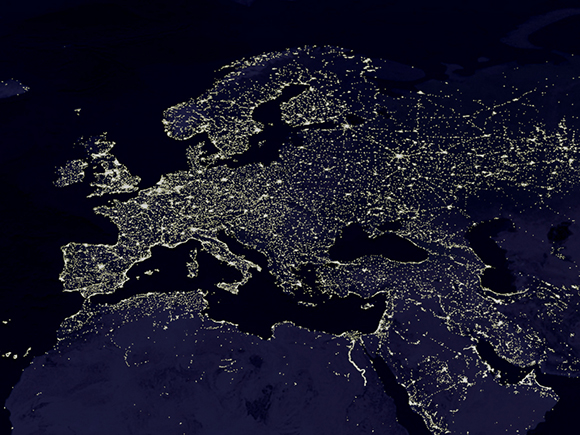
\includegraphics[width=0.7\textwidth]{02_wykresy/europe-nightlights-580.jpg}
\end{center}
\caption{Europa na nocnym zdjęciu satelitarnym}
\small{Żródło: \url{https://visibleearth.nasa.gov/view.php?id=55167}}
\label{fig:ntl}
\end{figure}

Dane NTL mogą zostać wykorzystane do pomiaru ubóstwa \citep{ntl2009}. Autorzy cytowanego artykułu dokonali oszacowania poziomu niedostatku dla wszystkich krajów świata w~ujęciu regionalnym. W Polsce obowiązywał wówczas podział na 49 województw i według mapy zamieszczonej na stronie projektu (\url{https://maps.ngdc.noaa.gov/viewers/dmsp/poverty.html}), wyznaczony wskaźnik ubóstwa nie przekraczał 30\%. Z kolei w Szwecji zweryfikowano istnienie korelacji pomiędzy danymi NTL, a innymi wskaźnikami ekonomicznymi. W przeprowadzonych badaniach wykazano, że istnieje silna zależność pomiędzy gęstością zaludnienia, a nocnym oświetleniem. W przypadku takich wskaźników jak odsetek zatrudnionych czy wielkość płacy korelacja była słabsza \citep{ntl2015}. 

Niestatystyczne źródło danych, pomocne przy analizie i ocenie poziomu ubóstwa, mogą stanowić informacje pozyskane z serwisów zawierających mapy, takich jak: Google Maps czy Open Street Map. Korzystając z API (interfejs programistyczny aplikacji) tych serwisów można pozyskać dane dotyczące obiektów użyteczności publicznej na danym obszarze takich jak np. szpitale, szkoły, supermarkety, itp. Ponadto serwisy te umożliwiają wyznaczenie odległości pomiędzy dwoma punktami uwzględniając rzeczywisty dystans drogowy. Może zostać także podany przybliżony czas podróży w zależności od wybranego środka transportu. Pozyskane dane można pobrać w formacie JSON lub XML i następnie przetwarzać. 

Źródła te nie są jednak wolne od wad. Przede wszystkim nie ma możliwości pobrania informacji historycznych --- można pozyskać wyłącznie aktualny stan bazy. Ponadto API Google Maps umożliwia wysłanie 2,5 tys zapytań dziennie, co w przypadku szczegółowych analiz przestrzennych może nie być wystarczające. Każde kolejne 1000 zapytań to koszt 0,50 dolara. Alternatywą może być wykorzystanie Open Street Map, które takich ograniczeń nie ma, ale z racji tego, że ten serwis jest rozwijany przez użytkowników i każdy może dodawać i usuwać obiekty topograficzne, pozyskane dane mogą być obarczone błędami.

Pobieranie danych ze źródeł internetowych w przypadku, kiedy nie istnieje API jest także możliwe dzięki zastosowaniu automatycznej ekstrakcji danych z sieci --- \textit{web-scrapingu}. Technika ta polega na napisaniu programu, który na podstawie znanej struktury strony internetowej zbiera wymagane informacje w zestandaryzowanej formie. W ten sposób można pozyskiwać dane z~zakresu m.in. cen produktów oraz rynku nieruchomości \citep{beresewicz2015}.

\section{Podsumowanie}

W rozdziale dokonano charakterystyki wykorzystywanych oraz potencjalnych źródeł informacji na temat ubóstwa. W pierwszej kolejności przedstawiono badania reprezentacyjne, w których respondenci między innymi deklarują wysokość dochodów lub wydatków. Ta informacja stanowi podstawę szacowania poziomu ubóstwa w Polsce i jest dostępna w czterech badaniach reprezentacyjnych. Dwa z nich realizowane są rokrocznie (BBGD i EU-SILC), Badanie Spójności Społecznej w cyklu czteroletnim, a Diagnoza Społeczna w dwuletnim. Wielkość próby tych badań umożliwia uzyskanie precyzyjnych oszacowań w bardzo ogólnych przekrojach terytorialnych --- najbardziej szczegółowym poziomem dostępności wyników są województwa.

Druga część rozdziału dotyczy spisów powszechnych. Jest to najpopularniejsze źródło zmiennych pomocniczych w estymacji pośredniej. Zbadanie wszystkich osób żyjących w Polsce w 2002 roku oraz odpowiednia duża próba stanowiąca 20\% populacji w NSP 2011 umożliwiły obserwację charakterystyk ludności, gospodarstw domowych, rodzin i mieszkań na poziomie powiatów. Niestety ze względu na duży koszt organizacji spisów powszechnych odbywają się one co dekadę.

Przeanalizowano także zakres danych zebranych w systemach informacyjnych Ministerstwa Finansów (MF) oraz Ministerstwa Pracy i Polityki Społecznej (MPiPS) w kontekście estymacji ubóstwa. MF w rejestrze PIT dysponuje danymi o dochodach podatników wraz z identyfikatorem terytorialnym. Dane te wykorzystywane są przez GUS w badaniu \textit{Wynagrodzenia w gospodarce narodowej} \citep{pbs2015}. Rejestr ten jednak mógłby być użyty także w badaniach nad ubóstwem ludności. Z kolei MPiPS dysponuje systemami wspomagającymi działania w obrębie bezrobocia rejestrowanego oraz świadczeń pomocy społecznej. W obu przypadkach zakres gromadzonych danych jest bardzo duży. Część z tych informacji w formie zagregowanej jest publikowana przez GUS. Są to m.in. informacje na temat bezrobocia rejestrowanego według różnych przekrojów rzeczowych i terytorialnych oraz wskaźniki korzystania z pomocy społecznej. Dane dostępne są na poziomie gmin. Niemniej liczba cech znajdująca się w tych rejestrach zachęca do przeprowadzenia bardziej szczegółowych analiz z wykorzystaniem np. modeli regresyjnych. Należy przy tym pamiętać, że rejestry administracyjne nie są źródłami statystycznymi co oznacza, że stosowane definicje i warianty cech mogą się różnić od tych stosowanych w systemach statystycznych \citep{roszka2012}.

Poruszono także kwestię pozyskania zmiennych dla statystyki małych obszarów z wykorzystaniem niestatystycznych źródeł. Można tutaj wyróżnić dane pochodzące ze zdjęć satelitarnych, a~także z Internetu (określanych często mianem \textit{Big Data}). Prowadzone badania pokazują wykorzystanie w estymacji pośredniej danych np. z Twittera. Innym źródłem mogą być mapy zawierające informacje o obiektach topograficznych znajdujących się na danym terenie, które można pobrać z wykorzystaniem API. W przypadku braku odpowiedniego interfejsu do pozyskania odpowiednich cech może służyć technika \textit{web-scrapingu}.

\chapter{Wybrane metody estymacji poziomu ubóstwa}
\section{Wprowadzenie}

Niniejsza część rozprawy zawiera opis wybranych estymatorów stosowanych w estymacji wskaźników ubóstwa na poziomach regionalnych i lokalnych. Rozdział składa się z czterech części. Pierwsza z nich jest poświęcona estymacji bezpośredniej --- klasycznemu podejściu wykorzystywanemu do uogólniania wyników pochodzących z badań reprezentacyjnych. Część druga i trzecia to opis wybranych metod dedykowanych estymacji wskaźników ubóstwa. W pierwszej kolejności zostało przedstawione podejście obszarowe, w którym poziom analizowanego wskaźnika ubóstwa w danym obszarze objaśniany jest zmiennymi mierzonymi na poziomie tego obszaru. Wykorzystuje się w tym celu charakterystyki społeczno-ekonomiczne dostępne m.in. w publicznych bazach statystycznych takich jak np. Bank Danych Lokalnych. Najpopularniejszym przedstawicielem tej grupy metod jest model Faya-Herriota \citep{fh1979}, który jest nieustannie rozwijany m.in. poprzez ujęcie w modelu macierzy sąsiedztwa i uwzględnienie w ten sposób czynnika przestrzennego \citep{pratesi2008}. Drugim rozważanym podejściem były modele jednostkowe, które bazują na modelowaniu dochodów lub wydatków gospodarstw domowych z wykorzystaniem danych jednostkowych pochodzących ze spisów powszechnych lub rejestrów administracyjnych. W rozdziale scharakteryzowano metodę empiryczną bayesowską (EB) \citep{ebp2010} oraz M-kwantylową (MQ) \citep{mq2006}. Ostatnia część rozdziału zawiera opis metod wykorzystywanych do diagnostyki oszacowań. Przedstawiona w pracy charakterystyka każdego z estymatorów obejmuje także opis metody estymacji błędu średniokwadratowego oszacowań. 

\section{Estymacja bezpośrednia}

Podstawowym narzędziem wykorzystywanym w estymacji parametrów populacji na podstawie badań reprezentacyjnych jest estymacja bezpośrednia. Przy odpowiednio licznej próbie estymator bezpośredni jest nieobciążony oraz efektywny \citep{rao2015}. Niemniej przy estymacji na niższym poziomie agregacji a tym samym przy mniej licznej próbie, estymator bezpośredni traci swoje własności. Pomimo tego oceny parametrów uzyskane z wykorzystaniem estymatora bezpośredniego są wykorzystywane jako wielkości wejściowe przy estymacji na poziomie obszaru oraz są punktem odniesieniu podczas oceny jakości oszacowań.

\subsection{Estymator Horvitza-Thompsona}\label{estymator-horvitza-thompsona}

Estymatorem stosowanym w badaniach reprezentacyjnych jest estymator bezpośredni zaproponowany przez Horvitza i Thompsona [\citeyear{ht1952}]. Niech $s$ oznacza próbę wylosowaną z populacji $U$, a~$s_d$ będzie podpróbą z obszaru $d$ o liczebności $n_d < N_d$. Przez $w_{dj}=\pi_{dj}^{-1}$ oznaczono wagę z próby będącą odwrotnością prawdopodobieństwa inkluzji pierwszego rzędu. Oszacowanie wartości globalnej w domenie $d$ uzyskuje się z wykorzystaniem wzoru:

\begin{equation}
\hat{Y}^{HT}_{d}=\sum\limits_{j=1}^{n_d}{y_{dj} w_{dj}},
\label{eq:ht}
\end{equation}

gdzie: $\hat{Y}^{HT}_{d}$ --- oszacowanie globalnej wartości cechy $Y$ w $d$-tej domenie, $y_{dj}$ --- wartość cechy $Y$ dla $j$-tej jednostki w $d$-tym obszarze, $w_{dj}$ --- wartość wagi wynikającej ze schematu losowania dla $j$-tej jednostki w $d$-tym obszarze.

W celu estymacji bezpośredniej wskaźników z rodziny FGT (przedstawionych w podrozdziale \ref{pr:wskazniki-ubostwa}) należy zmodyfikować formułę (\ref{eq:ht}) w następujący sposób:

\begin{equation}
\hat{F}_{\alpha d}^{HT}=N^{-1}_{d}\sum_{j \in s_d}{w_{dj}\left(\frac{z - E_{dj}}{z}\right)^{\alpha}I(E_{dj}<z)}, \; j=1, ..., N_d,
\label{eq:ht_fgt}
\end{equation}

gdzie: $w_{dj}$ --- wartość wagi wynikającej ze schematu losowania dla $j$-tej jednostki w $d$-tym obszarze, $N$ --- liczba osób w $d$-tym obszarze, $E_{dj}$ --- dochód $j$-tej jednostki, $z$ --- granica ubóstwa, $I(.)$ --- funkcja indykatorowa przyjmująca wartość 1 jeśli wyrażenie wewnątrz funkcji jest prawdziwe i 0 w przeciwnym przypadku.

Estymator bezpośredni wykorzystuje wyłącznie dane pochodzące z próby i dla dużych wartości $n_d$ jest nieobciążony i efektywny. Niemniej mała liczebność próby implikuje duże wartości wariancji. Ponadto ten sposób estymacji nie może zostać wykorzystany w przypadku, gdy dana domena w próbie nie jest w ogóle reprezentowana ($n_d=0$) \citep{molina2016}.

\subsection{Estymacja MSE w podejściu bezpośrednim}

Wariancja estymatora jest określana jako

\begin{equation}
V(\hat{\theta})=E[(\hat{\theta}-E[\hat{\theta}])^2]
\end{equation}

natomiast błąd średniokwadratowy (MSE)

\begin{equation}
MSE(\hat{\theta})=E[(\hat{\theta}-\theta)^2]
\end{equation}

Jeśli estymator jest nieobciążony tzn. $B(\hat{\theta})=E[\hat{\theta}-\theta]$ --- wówczas MSE i wariancja są sobie równe \citep{rao2015}. 

Estymator wariancji (MSE) nie wykorzystujący prawdopodobieństw inkluzji drugiego rzędu jest dany wzorem \citep{molina-marhuenda2015}:

\begin{equation}
\hat{V}\left(\hat{Y}^{HT}_d\right)=\frac{1}{N_d^2}\sum\limits_{j \in s_d}{w_{dj}(w_{dj}-1)Y^2_{dj}}.
\end{equation}

Wariancję estymatora bezpośredniego można także oszacowań metodą bootstrapową \citep{wolter2007}. W tym celu stosuje się procedurę, w ramach której losowanych jest $A$ niezależnych replikacji boostrapowych na podstawie próby podstawowej. Obserwacje, które zostają wylosowane oznaczane są odpowiednio symbolami $Y^*_{\alpha 1},\ldots, Y^*_{\alpha n}$, dla $\alpha=1,\ldots,A$ replikacji. Następnie dla każdej replikacji bootstrapowej, obliczana jest ocena estymatora $\hat{\theta}^{*}_\alpha$ szacowanego parametru. Wariancja estymatora dana jest wzorem:
\begin{equation}
\hat{V}(\hat{\theta})=\frac{1}{A-1}\sum\limits_{\alpha=1}^{A}{(\hat{\theta}^{*}_{\alpha}-\hat{\bar{\theta}}^*)^2},
\end{equation}
gdzie $\hat{\bar{\theta}}^*=\frac{1}{A}\sum\limits_{\alpha=1}^{A}{\hat{\theta}^{*}_{\alpha}}$.

%\section{Liniowy model mieszany}\label{liniowy-model-mieszany}

\section{Estymacja na poziomie obszaru}

Spośród technik estymacji pośredniej w pierwszej kolejności scharakteryzowano metody, które nie wymagają dostępu do danych jednostkowych z badania pełnego bądź rejestru administracyjnego, a wykorzystują wskaźniki dostępne w bazach statystycznych. Pomimo tego, że opisywane podejścia sięgają do roku 1979, cały czas są wykorzystywane i rozwijane w badaniach naukowych oraz stosowane przez statystykę publiczną \citep{saipe}.

\subsection{Model Faya-Herriota}

Model Faya-Herriota [\citeyear{fh1979}] jest modelem na poziomie obszaru, co oznacza że do jego aplikacji nie są wymagane dane jednostkowe pochodzące np. ze spisu powszechnego. Jest to niewątpliwa zaleta tego podejścia ponieważ dostęp do takich danych jest bardzo często niemożliwe, ze względu chociażby na zachowanie zasady tajemnicy statystycznej. Dostępność danych na poziomie badanej domeny jest z reguły dużo większa --- takie dane można pozyskać np. z Banku Danych Lokalnych, Eurostatu czy innych publicznych lub niepublicznych baz danych.

Budowa modelu Faya-Herriota przebiega w dwóch etapach \citep{torabi2008}. Pierwszy obejmuje założenie, że oszacowanie bezpośrednie ($\hat{\theta}_d$) parametru ($\theta_d$) jest nieobciążone i można je zapisać jako:

\begin{equation}
\hat{\theta}_d = \theta_d + e_d,
\end{equation}

gdzie $e_d\stackrel{ind}{\sim} N(0,\psi_{d})$. W praktyce wariancja $\psi_d$ nie jest znana, w związku z czym jest estymowana na podstawie próby lub obliczona z wykorzystaniem metody uogólnionej funkcji wariancji (GVF) \citep{wolter2007}.

W drugim etapie, model Faya-Herriota traktuje $\theta_d$ jako zmienną zależną w modelu liniowym z~jednym efektem losowym na poziomie obszaru:

\begin{equation}
\theta_d=x_d'\beta+u_d,
\end{equation}

gdzie $x_d$ --- wektor zmiennych niezależnych dla obszaru $d$ o wymiarach $p \times 1$, $\beta$ --- wektor parametrów regresji oraz $u_d$ --- efekt obszaru o $u_d\stackrel{iid}{\sim}N(0,\sigma^2_u)$.

Model zaproponowany przez Faya-Herriota jest wariantem modelu liniowego z efektem losowym (obszaru) \citep{fratczak2012}:

\begin{equation}
\theta_d=x_d'\beta+u_d+e_d,
\end{equation}

który można także przedstawić w formie macierzowej:

\begin{equation}
\mathbf{\theta}=\mathbf{X}\beta+\mathbf{u}+\mathbf{e}.
\end{equation}

W odniesieniu do estymacji stopy ubóstwa przyjmuje postać:

\begin{equation}
\hat{F}_{\alpha d}^{HT}=x_d^{T}\beta + u_d + e_d,\; d=1, ..., D,
\end{equation}

gdzie: $\hat{F}_{\alpha d}$ --- oszacowana wartość wskaźnika ubóstwa w obszarze $d$, $x_d^{T}$ --- wektor zmiennych niezależnych dla obszaru $d$ o wymiarach $p \times 1$, $u_d$ --- efekt obszaru o $u_d\stackrel{iid}{\sim}N(0,\sigma^2_u)$, $e_d$ --- błąd losowy $e_d\stackrel{ind}{\sim}N(0,\psi_d)$ o znanej wariancji $\psi_d$.

Najlepszy nieobciążony liniowy predyktor (ang. \textit{best linear unbiased predictor, BLUP}) wyrażony jest wzorem:

\begin{equation}
\tilde{F}_{\alpha d}^{FH}=x_d^{T}\tilde{\beta} + \tilde{u}_d = \gamma_d\hat{F}_{\alpha d}^{HT} + (1-\gamma_d)x_d^{T}\tilde{\beta},\; d=1, ..., D,
\end{equation}

gdzie: $\gamma_d=\frac{\sigma^2_u}{\sigma^2_u+\psi_d}$, a $\tilde{\beta}$ jest wyznaczone w wykorzystaniem ważonej metody najmniejszych kwadratów:

\begin{equation}
\tilde{\beta}=\left(\sum\limits_{d=1}^{D}{\gamma_d x_d x_d^T}\right)^{-1}\sum\limits_{d=1}^{D}{\gamma_d x_d \hat{F}_{\alpha d}^{HT}}.
\end{equation}

Estymator BLUP jest średnią ważoną oszacowania bezpośredniego $\hat{F}_{\alpha d}^{HT}$ oraz oszacowania syntetycznego regresyjnego $x_d^{T}\tilde{\beta}$. Waga $\gamma_d \in \left\langle 0,1\right\rangle$ mierzy niepewność wynikającą z opisu szacowanej wartości przez model regresyjny. W zależności od wariancji z próby $\psi_d$ oraz wariancji międzyobszarowej $\sigma_u^2$ większy bądź mniejszy udział będzie przypisywany szacunkowi bezpośredniemu \citep{boonstra2011}.

W praktyce wartość $\sigma_u^2$ nie jest znana i należy ją estymować. W tym celu można wykorzystać szereg metod: metodę Faya-Herriota lub Prasada-Rao, a także metodę największej wiarygodności oraz metodę największej wiarygodności z ograniczeniami \citep{prasad1990}. Zastępując $\sigma_u^2$ wartością oszacowaną $\hat{\sigma}^2_u$ otrzymuje się empiryczny najlepszy nieobciążony liniowy predyktor (EBLUP):

\begin{equation}
\hat{F}_{\alpha d}^{FH}=x_d^{T}\hat{\beta} + \hat{u}_d = \hat{\gamma}_d\hat{F}_{\alpha d}^{HT} + (1-\hat{\gamma}_d)x_d^{T}\hat{\beta},\; d=1, ..., D,
\end{equation}

oraz 

\begin{equation}
\hat{\beta}=\left(\sum\limits_{d=1}^{D}{\hat{\gamma}_d x_d x_d^T}\right)^{-1}\sum\limits_{d=1}^{D}{\hat{\gamma}_d x_d \hat{F}_{\alpha d}^{HT}},
\end{equation}

gdzie $\hat{\gamma}_d=\frac{\hat{\sigma}^2_u}{\hat{\sigma}^2_u+\psi_d}$.

Dla niereprezentowanych w próbie domen szacunek wyznacza się wykorzystując jedynie podejście pośrednie, nie korzystając z oszacowań bezpośrednich.

\begin{equation}
\hat{F}_{\alpha d}^{FH}=x_d^{T}\hat{\beta},\; d=1, ..., D,
\end{equation}

Uzyskane w ten sposób oceny estymatorów określa się mianem syntetycznych \citep{rao2015}.

\subsection{Przestrzenny model Faya-Herriota}

Przestrzenny model Faya-Herriota \citep{pratesi2008} zakłada uwzględnienie w klasycznym modelu Faya-Herriota macierzy sąsiedztwa oraz wyznaczonego na jej podstawie współczynnika autokorelacji przestrzennej efektów losowych. Ogólna postać tego modelu jest wówczas następująca:

\begin{equation}
\hat{F}_{\alpha d}^{HT}=x_d^{T}\beta + (I-\rho W)^{-1}u_d + e_d,\; d=1, ..., D,
\end{equation}

gdzie: $\hat{F}_{\alpha d}$ --- oszacowania wartość wskaźnika ubóstwa w obszarze $d$, $x_d^{T}$ --- wektor zmiennych niezależnych dla obszaru $d$ o wymiarach $p \times 1$, $\rho$ --- współczynnik autokorelacji przestrzennej, $W$~--- macierz sąsiedztwa, $u_d$ --- efekt obszaru o $u_d\stackrel{iid}{\sim}N(0,\sigma^2_u)$, $e_d$ --- błąd losowy $e_d\stackrel{ind}{\sim}N(0,\psi_d)$ o~znanej wariancji $\psi_d$.

Macierz $W$ jest macierzą sąsiedztwa pomiędzy analizowanymi obszarami, z kolei $\rho$ jest miarą powiązań przestrzennych pomiędzy efektami losowymi w sąsiadujących obszarach. W oryginalnej macierzy sąsiedztwa $W^0$ elementy diagonalne są równe 0, natomiast pozostałe elementy macierzy przyjmują wartość równą 1 w przypadku gdy dwa obszary ze sobą sąsiadują, a 0 w przeciwnym razie. Macierz $W$ otrzymuje się na podstawie $W^0$ poprzez podzielenie każdego elementu w wierszu przez sumę wiersza. W ten sposób uzyskuje się macierz wierszowo-standaryzowaną, w której suma każdego wiersza jest równa 1.

Estymatorem tego modelu jest przestrzenny najlepszy liniowy nieobciążony predyktor (Spatial BLUP):

\begin{multline}
\tilde{F}_{\alpha d}^{SFH}=x_d^{T}\tilde{\beta}+b_{d}^{T}\left\{\sigma_u^2\left[(I-\rho W)(I-\rho W^T)\right]^{-1}\right\} \\ \times \left\{diag(\psi_d)+\sigma_u^2\left[(I-\rho W)(I-\rho W^T)\right]^{-1}\right\}^{-1}(\hat{F}_{\alpha d}^{HT}-x_d^{T}\tilde{\beta}),\; d=1, ..., D,
\end{multline}

gdzie: $b_d^T$ jest wektorem $1 \times D$ z wartością 1 na $d$-tej pozycji, natomiast

\begin{equation}
\tilde{\beta}=\left(\sum\limits_{d=1}^{D}{v_d x_d x_d^T}\right)^{-1}\sum\limits_{d=1}^{D}{v_d x_d \hat{F}_{\alpha d}^{HT}},
\end{equation}

gdzie $v_d=diag(\psi_d)+\sigma_u^2\left[(I-\rho W)(I-\rho W^T)\right]^{-1}.$

Powyższy estymator zależy od dwóch nieznanych wartości: $\sigma_u^2$ oraz $\rho$. Zastąpienie tych wartości oszacowaniami prowadzi do wyznaczenia wzoru na estymator SEBLUP:

\begin{multline}
\hat{F}_{\alpha d}^{SFH}=x_d^{T}\hat{\beta}+b_{d}^{T}\left\{\hat{\sigma}_u^2\left[(I-\hat{\rho} W)(I-\hat{\rho} W^T)\right]^{-1}\right\} \\ \times \left\{diag(\psi_d)+\hat{\sigma}_u^2\left[(I-\hat{\rho} W)(I-\hat{\rho} W^T)\right]^{-1}\right\}^{-1}(\hat{F}_{\alpha d}^{HT}-x_d^{T}\hat{\beta}),\; d=1, ..., D.
\end{multline}

Podobnie, jak w przypadku klasycznego modelu Faya-Herriota, także w wariancie przestrzennym do wyznaczenia oszacowania w niereprezentowanych w próbie domenach wykorzystuje się wyłącznie estymację syntetyczną:

\begin{equation}
\hat{F}_{\alpha d}^{SFH}=x_d^{T}\hat{\beta}, \; d=1, ..., D.
\end{equation}

\subsection{Estymacja MSE w podejściu obszarowym}

Błąd średniokwadratowy (MSE) powyższych estymatorów można zapisać jako sumę:

\begin{equation}
MSE(\hat{F}_{\alpha d}^{FH})=g_{1d}(\hat{\sigma}_u^2)+g_{2d}(\hat{\sigma}_u^2)+2g_{3d}(\hat{\sigma}_u^2)
\end{equation}

lub

\begin{equation}
MSE(\hat{F}_{\alpha d}^{SFH})=g_{1d}(\hat{\sigma}_u^2,\hat{\rho})+g_{2d}(\hat{\sigma}_u^2,\hat{\rho})+2g_{3d}(\hat{\sigma}_u^2,\hat{\rho}),
\end{equation}

gdzie:

\begin{equation}
g_{1d}(\hat{\sigma}_{u}^{2})=\hat{\gamma}_{d}\psi_{d},
\end{equation}

\begin{equation}
g_{2d}(\hat{\sigma}_{u}^{2})=(1-\hat{\gamma_{d}})^2 x_{d}^{T}\left[\sum\limits_{d=1}^{D}{x_{d}x_{d}^{T}}/(\psi_{d}+\hat{\sigma}_{u}^{2})\right]^{-1}x_{d},
\end{equation}

oraz

\begin{equation}
g_{3d}(\hat{\sigma}_{u}^{2})=\psi_{d}^{2}(\psi_{d}+\hat{\sigma}_{u}^{2})^{-3}\bar{V}(\hat{\sigma}_{u}^{2}).
\end{equation}

Asymptotyczna wariancja $\bar{V}(\hat{\sigma}_{u}^{2})$ jest wyznaczana według wzoru:

\begin{equation}
\bar{V}(\hat{\sigma}_{u}^{2})=2D^{-2}\sum\limits_{d=1}^{D}{(\hat{\sigma}_{u}^{2}+\psi_{d})^2}.
\end{equation}

Składnik MSE $g_{1d}$ odpowiada za błąd oszacowania $\psi_d$, $g_{2d}$ za błąd oszacowania parametrów $\beta$, a $g_{3d}$ jest składnikiem odpowiadającym za błąd oszacowania $\sigma_u^2$ w klasycznym modelu Faya-Herriota lub $\sigma_u^2$ i $\rho$ w przestrzennym modelu Faya-Herriota \citep{singh2005}.

Do estymacji wariancji można także wykorzystać parametryczną metodę bootstrap \citep{gonzales2008}.

Algorytm estymacji jest następujący:

\begin{enumerate}
\item dopasowanie oryginalnego modelu otrzymując oszacowanie $\hat{\sigma}_u^2$ oraz $\hat{\beta}$,
\item wygenerowanie wektora $\mathbf{u^*}$ o rozkładzie $N(0, \hat{\sigma}_u)$ oraz obliczenie $\mathbf{\theta^*}=\mathbf{X}\hat{\beta}+\mathbf{u^*}$,
\item wygenerowanie wektora $\mathbf{e^*}$ o rozkładzie $N(0, \sqrt{\psi})$,
\item skonstruowanie wektora danych bootstrapowych $\mathbf{\hat{\theta}^*}=\mathbf{\theta^*}+\mathbf{e^*}=\mathbf{X}\hat{\beta}+\mathbf{u^*}+\mathbf{e^*}$,
\item dopasowanie modelu do danych bootstrapowych $\mathbf{\hat{\theta}^*}$ w celu otrzymania nowych oszacowań $\hat{\sigma}_u^{2*}$ oraz $\hat{\beta}^{*}$ --- traktując wektor $\psi$ jako wartości prawdziwe,
\item wyznaczenie $\hat{\theta}^{*B}$ uwzględniając wartości wyznaczone w punkcie 5,
\item powtórzenie kroków 2-6 $B$ razy. Zakładając, że $\theta^{*(b)}$ oznacza znane wartości parametru, a~$\mathbf{\hat{\theta}}^{*(b)}$ oszacowania EBLUP otrzymane w $b$-tej replikacji bootstrapowej,
\item estymatorem wariancji jest: 
\begin{equation}
\hat{V}(\hat{\theta})=B^{-1}\sum\limits_{b=1}^{B}{[\hat{\theta}^{*(b)}-\theta^{*(b)}]^2}.\end{equation}
\end{enumerate}

Przedstawiony algorytm można także wykorzystać do oszacowania wariancji estymatora SEBLUP. Wówczas należy dodatkowo uwzględnić macierz odległości $W$ oraz współczynnik autokorelacji przestrzennej $\rho$ \citep{pratesi2007}.

\section{Estymacja na poziomie jednostki}

Podejście jednostkowe jako zmienną zależną przyjmuje wektor dochodów lub wydatków gospodarstw domowych z wykorzystaniem danych jednostkowych pochodzących z badań pełnych lub rejestrów administracyjnych. W tym przypadku dostępność zmiennych niezależnych jest dużo mniejsza od tej występującej dla modeli obszarowych. Estymacja wskaźnika ubóstwa w przypadku tych metod polega na tworzeniu, z wykorzystaniem symulacji Monte Carlo, pseudo-populacji, które stanowią podstawę estymacji wskaźników ubóstwa. Ze względu na wymaganą dużą liczbę replikacji oraz wykorzystywanie baz danych znacznych rozmiarów estymacja wariancji w podejściu jednostkowym jest rozbudowanym obliczeniowo działaniem, co przekłada się przede wszystkim na długotrwały proces przetwarzania danych.

\subsection{Metoda empiryczna bayesowska}

Metoda empiryczna bayesowska (EB) jest stosunkowo nowym podejściem przedstawionym w artykule \textit{Small area estimation of poverty indicators} \citep{ebp2010}. Polega na dopasowaniu liniowego modelu mieszanego opisującego dochód na poziomie gospodarstwa domowego na podstawie danych z badania reprezentacyjnego. Uzyskane oszacowania parametrów $\beta$ oraz wariancje efektów losowych są następnie wykorzystywane w generowaniu teoretycznych wartości dochodu dla jednostkowych wartości \textit{zmiennych pomocniczych} pochodzących z badania pełnego.

Dany jest wektor $y=(y_1,...,y_N)'$ zawierający wartości zmiennej losowej powiązanej z $N$ jednostkami skończonej populacji. Niech $y_s$ będzie fragmentem wektora $y$ zawierającym informacje z wylosowanej próby $s$, a $y_r$ wektorem elementów spoza próby. Po uporządkowaniu elementów można zapisać, że $y=(y'_s, y'_r)$. Celem jest oszacowanie wartości funkcji $\delta=h(y)$ zmiennej losowej $y$ z wykorzystaniem danych z próby $y_s$. Dla estymatora $\delta$ błąd średniokwadratowy (MSE) jest dany wzorem:

\begin{equation}
\text{MSE}(\hat{\delta})=E_y\{(\hat{\delta}-\delta)^2\},
\label{eq:msebp}
\end{equation}

gdzie $E_y$ oznacza wartość oczekiwaną z uwzględnieniem łącznego rozkładu wektora $y$. Najlepszym estymatorem (ang. \textit{best predictor, BP}) parametru $\delta$ jest funkcja na $y_s$, która minimalizuje (\ref{eq:msebp}) i jest dana warunkową wartością oczekiwaną:

\begin{equation}
\hat{\delta^{B}}=E_{y_{r}}(\delta|y_s),
\label{eq:bp}
\end{equation}

gdzie wartość oczekiwana uwzględnia warunkowy rozkład $y_r$. Warto zauważyć, że ten estymator jest nieobciążony ponieważ:

\begin{equation}
E_{y_{s}}(\hat{\delta}^B)=E_{y_{s}}\{E_{y_{r}}(\delta|y_s)\}=E_y(\delta).
\end{equation}

Zwykle $\hat{\delta}^B$ zależy od wektora $\theta$ nieznanych parametrów modelu. Wówczas empiryczny BP $\delta$ otrzymuje się poprzez zastąpienie $\theta$ odpowiednim estymatorem $\hat{\theta}$ i następne oszacowanie (\ref{eq:bp}) przyjmując $\theta=\hat{\theta}$.

Poniżej zaprezentowano sposób otrzymania oszacowania BP dla rodziny wskaźników ubóstwa FGT dla małych domen. Zakładamy transformację zmiennej dochodowej $E_{dj}$ według formuły $Y_{dj}=T(E_{dj})$, biorąc pod uwagę, że wektor $y$ zawiera wartości transformowanej zmiennej $Y_{dj}$ dla wszystkich jednostek populacji tak, że $y \sim N(\mu, V)$. Wówczas zmienną losową 

\begin{equation}
\hat{F}_{\alpha d j}=\left(\frac{z - E_{dj}}{z}\right)^{\alpha}I(E_{dj}<z),\; j=1, ..., N_d.
\label{eq:fgt2}
\end{equation}

można wyrazić w kontekście $Y_{dj}$ jako:

\begin{equation}
F_{\alpha d j}=\left(\frac{z-T^{-1}(Y_{dj})}{z}\right)^{\alpha}I\left\{T^{-1}(Y_{dj})<z\right\}=:h_{\alpha}(Y_{dj}),\qquad \text{j=1,...,$N_d$}.
\end{equation}

Wobec tego miara ubóstwa (\ref{eq:fgt}) jest nieliniową funkcją wektora $y$. Przyjmując za $\delta=F_{\alpha d}$ i~podstawiając do (\ref{eq:bp}) najlepszym estymatorem (BP) parametru $F_{\alpha d}$ jest:

\begin{equation}
\hat{F}^{B}_{\alpha d}=E_{y_{r}}(F_{\alpha d}|y_s)
\label{eq:bpexp}
\end{equation}

Dekomponując $F_{\alpha d}$ (\ref{eq:fgt}) na jednostki wylosowane i spoza próby otrzymuje się:

\begin{equation}
F_{\alpha d}=\frac{1}{N_d}\left\{\sum\limits_{j \in s_d}{F_{\alpha dj}}+\sum\limits_{j \in r_d}{F_{\alpha dj}}\right\}
\label{eq:dec1}
\end{equation}

Uwzględniając warunkową wartość oczekiwaną formuły (\ref{eq:dec1}) i wprowadzając ją do wnętrza sumy, estymator wskaźnika ubóstwa przyjmuje postać:

\begin{equation}
\hat{F}^B_{\alpha d}=\frac{1}{N_d}\left\{\sum\limits_{j \in s_d}{F_{\alpha dj}}+\sum\limits_{j \in r_d}{\hat{F}^B_{\alpha dj}}\right\}
\label{eq:dec2}
\end{equation}

gdzie $\hat{F}^B_{\alpha dj}$ jest najlepszym estymatorem $F_{\alpha d j}=h_{\alpha}(Y_{dj})$ danym przez

\begin{equation}
\hat{F}^B_{\alpha dj}=E_{y_{r}}[h_{\alpha}(Y_{dj})|y_s]=\int_{IR}{h_{\alpha}(y)f_{Y_{dj}}(y|y_s)}\text{d}y,\qquad j \in r_d.
\label{eq:bpcalka}
\end{equation}

$f_{Y_{dj}}(y|y_s)$ jest warunkową gęstością $Y_dj$ wektora $y_s$. Wartość oczekiwana (\ref{eq:bpcalka}) nie może zostać wyliczona bezpośrednio z powodu złożoności $h_{\alpha}(y)$. Jednakże w przypadku, gdy $y=(y'_s,y'_r)'$ ma rozkład normalny ze średnią daną wektorem $\mu=(\mu'_s,\mu'_r)'$, macierz kowariancji jest zdekomponowana jako:

\begin{equation}
V=
\begin{bmatrix}
V_s & V_{sr}\\
V_{rs} & V_r
\end{bmatrix},
\end{equation}

a warunkowy rozkład $y_r$ pod warunkiem $y_s$ dany jest przez

\begin{equation}
y_r|y_s \sim N(\mu_{r|s},V_{r|s}),
\label{eq:condyr}
\end{equation}

gdzie:

\begin{equation}
\mu_{r|s}=\mu_r+V_{rs}V_{s}^{-1}(y_s-\mu_s) \qquad \text{i} \qquad V_{r|s}=V_r-V_{rs}V_s^{-1}V_{sr}.
\label{eq:distyr}
\end{equation}

Wówczas empiryczne przybliżenie rozwiązania (\ref{eq:bpcalka}) jest możliwe z wykorzystaniem symulacji Monte Carlo o dużej liczbie $L$ wektorów $y_r$ wygenerowanych z (\ref{eq:condyr}).

Niech $Y_{dj}^{(\ell)}$ oznacza wartości zmiennej $Y_{dj}$, $j\in r_d$ spoza próby otrzymane w $\ell$ symulacjach $\ell=1,...,L$. Przybliżenie Monte Carlo najlepszego estymatora (BP) $Y_{dj}$ dla $j \in r_d$ jest wyrażone jako:

\begin{equation}
\hat{F}^{B}_{\alpha d j}=E_{y_{r}}[h_{\alpha}(Y_{dj})|y_s]\approx \frac{1}{L}\sum\limits_{\ell=1}^{L}{h_{\alpha}(Y_{dj}^{(\ell)})}, \qquad j \in r_d.
\label{eq:bpmc}
\end{equation}

Końcowym estymatorem jest $\hat{F}_{\alpha d j}^{EB}$ będący najlepszym empirycznym predyktorem (EBP) parametru $F_{\alpha d j}$. Ostatecznie EBP miary ubóstwa $F_{\alpha d}$ jest określony wzorem:

\begin{equation}
\hat{F}^{EB}_{\alpha d}=\frac{1}{N_d}\left\{\sum\limits_{j \in s_d}{F_{\alpha dj}}+\sum\limits_{j \in r_d}{\hat{F}^{EB}_{\alpha dj}}\right\}.
\label{eq:ebp}
\end{equation}

Zamiast wprowadzać wartość oczekiwaną do sumy tak jak w (\ref{eq:dec2}), wartość oczekiwana (\ref{eq:bpexp}) może być bezpośrednio przybliżona przez symulację Monte Carlo \citep{ebp2010}. Pozwala to na estymację praktycznie dowolnego parametru dla domeny $\delta_d=h(y_d)$ bez potrzeby wydzielania $\sum\limits_{j}{h(Y_{dj})}$. Przykładami estymowanych parametrów są kwantyle zmiennej dochodowej $E_{dj}=T^{-1}(Y_dj)$. Wówczas procedura zastosowania metody EB w estymacji parametru dla domeny $\delta_d=h(y_d)$ jest następująca:

\begin{enumerate}
\item estymacja nieznanych parametrów rozkładu $\theta$ transformowanego wektora $y$ wykorzystując dane z próby $y_s$,
\item wygenerowanie $L$ wektorów spoza próby $y_r^{(\ell)},\ell=1,...,L$ na podstawie (\ref{eq:condyr}) i (\ref{eq:distyr}) zastępując $\theta$ estymatorem $\hat{\theta}$ uzyskanym w punkcie 1,
\item rozszerzenie każdego z $L$ wygenerowanych wektorów $y_r^{(\ell)}$ danymi z próby $y_s$ do postaci wektora populacji $y^{\ell}=(y'_s,(y_r^{(\ell)})')', \ell=1,...,L$,
\item wyznaczenie wartości parametru dla domeny $\delta^{(\ell)}_d=h(y_d^{(\ell)})$ wykorzystując elementy wektora $y^{(\ell)}$ dla $d$-tej domeny - $y_d^{\ell}=(y'_{ds},(y_{dr}^{(\ell)})')'$,
\item przybliżenie Monte Carlo estymatora EBP parametru $\delta_d$ otrzymuje się poprzez uśrednienie wartości parametru dla domeny na podstawie $L$ pseudo-populacji:
\begin{equation}
\delta^{EB}_d=\frac{1}{L}\sum\limits_{\ell=1}^{L}{\delta_d^{(\ell)}}.
\end{equation}
\end{enumerate}

%Jedyne wymaganie wobec tej metody jest takie, że rozkład transformowanej zmiennej $Y_{dj}=T(E_{dj})$ jest znany i warunkowy rozkład $y_r|y_s$ jest różniczkowalny.

\subsubsection{Liniowy model regresji z zagnieżdżonym składnikiem losowym}

W tej części zostanie wprowadzony model nadpopulacji $\xi$ oparty na liniowym modelu regresji z zagnieżdżonym błędem (Battese, Harter i Fuller, 1988), który może zostać wykorzystany do oszacowania (\ref{eq:ebp}). Model opisuje liniową dla wszystkich domen relację pomiędzy transformowaną zmienną dochodową $Y_{dj}$, a wektorem $x_{dj}$ zawierającym wartości $p$ zmiennych niezależnych, a~także uwzględnia losowy efekt dla domeny $u_d$ wraz z resztami $e_{dj}$:

\begin{equation}
\xi:\;Y_{dj}=x'_{dj}\beta+u_d+e_{dj},\qquad j=1,..,N_d, \qquad d=1,...,D,
\label{eq:modelBHF}
\end{equation}

gdzie: $u_d\stackrel{iid}{\sim}N(0,\sigma^2_u)$ i $e_{dj}\stackrel{iid}{\sim}N(0,\sigma^2_e)$, a $u_d$ oraz $e_{dj}$ są niezależne.

Wektory i macierze otrzymane poprzez wydzielenie elementów dla domeny $d$:

\begin{equation}y_d=col_{1 \leq j \leq N_d}(Y_{dj}),\qquad e_d=col_{1 \leq j \leq N_d}(e_{dj}),\qquad X_d=col_{1 \leq j \leq N_d}(x'_{dj})\end{equation}.

Wówczas wektor $y_d, d=1,...,D$ jest niezależny z $y_d \sim N(\mu_d, V_d)$, gdzie:

\begin{equation}
\mu_d=X_d\beta \qquad \text{i} \qquad V_d=\sigma_u^2 1_{N_d}1'_{N_d}+\sigma_e^2 I_{N_d},
\end{equation}

gdzie $1_k$ oznacza kolumnowy wektor jedynek o rozmiarze $k$, a $I_k$ jest macierzą jednostkową $k \times k$.

Rozważana jest dekompozycja $y_d$ na jednostki wylosowane i te spoza próby $y_d=(y'_{ds},y'_{dr})'$ wprzypadku $n_d>0$ i podobnie dla $X_d, \mu_d$ i $V_d$. Rozkład $y_{dr}$ określony przez jednostki w próbie $y_{ds}$ jest w takim przypadku następujący:

\begin{equation}
y_{dr}|y_{ds} \sim N(\mu_{dr|s}, V_{dr|s}),
\end{equation}

gdzie

\begin{equation}
\mu_{dr|s}=X_{dr}\beta + \sigma^2_u 1_{N_d-n_d}1'_{n_d}V^{-1}_{ds}(y_{ds}-X_{ds}\beta),
\label{eq:mudrs}
\end{equation}

\begin{equation}
V_{dr|s}=\sigma^2_u(1-\gamma_d)1_{N_d-n_d}1'_{N_d-n_d}+\sigma^2_eI_{N_d-n_d},
\label{eq:vdrs}
\end{equation}

dla $V_{ds}=\sigma^2_u1_{n_d}1'_{n_d}+\sigma^2_eI_{n_d}$ oraz $\gamma_d=\sigma^2_u(\sigma^2_u+\sigma^2_e/n_d)^{-1}$. Należy zauważyć, że $y_{dr}|y_{ds}$ i $y_{dr}|y_s$ mają taki sam rozkład w związku z niezależnością $y_d, d=1,...,D$. Załóżmy, że podział $\Omega_d$na $s_d$ i $r_d$ jest znany oraz, że zmienne niezależne $x_{dj}$ powiązane z $j \in r_d$ są znane.

Zastosowanie przybliżenia Monte Carlo (\ref{eq:bpmc}) pociąga za sobą symulację $D$ wektorów $y_{dr}$ o~rozmiarze $N_d-n_d, d=1,...,D$ o wielowymiarowym rozkładzie normalnym. Powtórzenie tego procesu $L$ razy sprawia, że jest on wymagający obliczeniowo, a nawet niewykonalny dla dużych $N_d$. Można tego uniknąć zauważając, że macierz $V_{dr|s}$ (\ref{eq:vdrs}) odpowiada macierzy kowariancji wektora $y_{dr}$ wygenerowanego przez model

\begin{equation}
y_{dr}=\mu_{dr|s}+v_d1_{N_d-n_d}+\varepsilon_{dr}
\label{eq:ydr}
\end{equation}

z nowym efektem losowym $v_d$ oraz błędem $\varepsilon_{dr}$, które są niezależne o rozkładach:

\begin{equation}
v_d \sim N\{0,\sigma^2_u(1-\gamma_d)\},\qquad d=1,..,D, \qquad \varepsilon \sim N(0_{N_d-n_d},\sigma^2_eI_{N_d-n_d}).
\end{equation}

Wykorzystując (\ref{eq:ydr}), zamiast generowania wektora $y_{dr}$ o wielowymiarowym rozkładzie normalnym wystarczy wygenerować jednowymiarowe zmienne $v_d \sim N\{0,\sigma^2_u(1-\gamma_d)\}$ i $\varepsilon_{dj} \sim N(0, \sigma^2_e)$ niezależnie dla $j \in r_d$ i wówczas uzyskać odpowiadające elementy wektora $y_{dj}, j \in r_d$ z (\ref{eq:ydr}) wykorzystując $\mu_{dr|s}$ dane przez (\ref{eq:mudrs}). Jak wspomniano wcześniej, w praktyce parametry modelu $\theta=(\beta',\sigma^2_u,\sigma^2_e)'$ są zastępowane przez odpowiednie estymatory $\hat{\theta}=(\hat{\beta}',\hat{\sigma}^2_u,\hat{\sigma}^2_e)'$ i wówczas wartości zmiennej $Y_{dj}$ są generowane rozkładu normalnego o odpowiednim odchyleniu standardowym.

Jeśli domena $d$ nie znalazła się w próbie, wówczas wartości $Y^{(\ell)_{dj}}$ dla $j=1,...,N_d$ są generowane metodą bootstrap z wykorzystaniem $Y_{dj}=x'_dj\hat{\beta}+u^*_d+e^*_{dj}$, gdzie $u^*_d\stackrel{iid}{\sim}N(0,\hat{\sigma}^2_u)$ i~$e^*_{dj}\stackrel{iid}{\sim}N(0,\hat{\sigma^2_e})$ i $u^*_d$ jest niezależne od $e^*_{dj}$. Wzór (\ref{eq:bpmc}) jest wówczas wykorzystany do otrzymania estymatora $\hat{F}^{EB}_{\alpha dj}$ dla $F_{\alpha d j}$ i estymatora EB $F_{\alpha d}$ jako:

\begin{equation}
\hat{F}_{\alpha d}^{EB}=N_d^{-1}\sum\limits_{j=1}^{N_d}{\hat{F}^{EB}_{\alpha dj}}
\label{eq:febad2}
\end{equation}

Estymator (\ref{eq:febad2}) jest syntetycznym estymatorem jeśli żadna jednostka nie jest obserwowana w domenie $d$.

%Na rysunku \ref{fig:eb} przedstawiono schemat estymacji wskaźnika ubóstwa z wykorzystaniem estymatora EB.

% \begin{figure}[ht]
% \includegraphics[width=\textwidth]{03_wykresy/EB.pdf}
% \caption{Algorytm estymacji wskaźnika ubóstwa z wykorzystaniem estymatora EB}
% \small{Źródło: opracowanie własne na podstawie \citep{ebp2010}.}
% \label{fig:eb}
% \end{figure}

\subsection{Estymacja MSE w podejściu EB metodą bootstrap}

Błąd średniokwadratowy $\hat{F}^{EB}_{\alpha d}$ można zapisać jako:

\begin{equation}
\text{MSE}(\hat{F}^{EB}_{\alpha d})=E_{\xi}(\hat{F}^{EB}_{\alpha d}-F_{\alpha d})^2,
\label{eq:mseeb1}
\end{equation}

gdzie $E_{\xi}$ oznacza wartość oczekiwaną z uwzględnieniem modelu $\xi$. Wzór (\ref{eq:mseeb1}) można zdekomponować w następujący sposób:

%Należy zauważyć, że parametr $F_{\alpha d}$ jest zmienną losową, więc tradycyjna dekompozycja MSE na kwadrat obciążenia i wariancję $\hat{F}^{EB}_{\alpha d}$ nie ma racji bytu. 

\begin{equation}
\text{MSE}(\hat{F}^{EB}_{\alpha d})=V_{\xi}(\hat{F}^{EB}_{\alpha d}-F_{\alpha d})+\{E_{\xi}(\hat{F}^{EB}_{\alpha d}-F_{\alpha d})^2\},
\label{eq:mseeb2}
\end{equation}

gdzie: $V_{\xi}$ oznacza wariancję modelu, a $E_{\xi}(\hat{F}^{EB}_{\alpha d}-F_{\alpha d})^2$ jest modelowym obciążeniem $\hat{F}^{EB}_{\alpha d}$. 

%Dopóki modelowe obciążenie `'najlepszego'`estymatora $\hat{F}^{B}_{\alpha d}$ jest równe zero, kwadrat obciążenia'`najlepszego empirycznego'' estymatora $\hat{F}^{EB}_{\alpha d}$ w (\ref{eq:mseeb2}) jest zwykle bardzo małe w odniesieniu do wariancji szacowanego błędu $\hat{F}^{EB}_{\alpha d}-F_{\alpha d}$, kiedy $D$ jest duże. W takim przypadku MSE jest zdominowane prze składnik wariancji (\ref{eq:mseeb2}).

Analityczne przybliżenia MSE są trudne do otrzymania w przypadku złożonych parametrów takich jak miary ubóstwa. Wówczas można wykorzystać parametryczny bootstrap dla skończonych populacji \citep{gonzales2008}. Poniżej przedstawiony jest algorytm tej metody:

\begin{enumerate}
\item dopasowanie modelu (\ref{eq:modelBHF}) do danych z próby ($y_s, X_s$), w celu otrzymania oszacowania $\hat{\beta}, \hat{\sigma}^2_u, \hat{\sigma}^2_e$ parametrów $\beta, sigma^2_u, \sigma^2_e$,
\item wygenerowanie wektora $u^*_d\stackrel{iid}{\sim}N(0,\hat{\sigma}^2_u), d=1,...,D$ i niezależnie $e^*_{dj}\stackrel{iid}{\sim}N(0,\hat{\sigma}^2_e), j=1,...,N_d, d=1,...,D$,
\item skonstruowanie bootstrapowego modelu nadpopulacji $\xi^*$ wykorzystującego $u^*_d, e^*_{dj}, x_{dj}, \hat{\beta}$:
\begin{equation}
\xi^*:Y^*_{dj}=x'_{dj}\hat{\beta}+u^*_{d}+e^*_{dj},\qquad j=1,...,N_d,\qquad d=1,...,D,
\label{eq:modelBHFboot}
\end{equation}
\item wygenerowanie $B$ niezależnych i o identycznym rozkładzie pseudo-populacji bootstrapowych  $\{Y^{*(b)}_{dj};\;j=1,...,N_d,\;d=1,...,D\}$ na podstawie modelu (\ref{eq:modelBHFboot}), a następnie wyznaczenie odpowiednich parametrów $F^{*(b)}_{\alpha d}=N^{-1}_{d}\sum\limits_{j=1}^{N_d}{F^{*(b)}_{\alpha dj}}$, gdzie $F^{*(b)}_{\alpha dj}=h_{\alpha}(Y^{*(b)}_{dj}),b=1,...,B$,
\item wylosowanie próby $s \subset U$ z każdej bootstrapowej populacji $b$ wygenerowanej w punkcie 4~i~wyznaczenie bootstrapowego EBP $F^{EB*(b)}_{\alpha d},b=1...,B$ tak jak opisano wcześniej, wykorzystując dane z próby $y^*_s$ i znane wartości populacji $x_{dj}$,
\item przybliżenie Monte Carlo estymatora $\text{MSE}_*(\hat{F}^{EB*}_{\alpha d})=E_{\xi*}(\hat{F}^{EB*}_{\alpha d}-F^*_{\alpha d})^2$ parametru $\hat{F}^{EB}_{\alpha d}$ jest obliczane jako:
\begin{equation}
\text{mse}_*(\hat{F}^{EB}_{\alpha d})=\frac{1}{B}\sum\limits_{b=1}^{B}(\hat{F}^{EB*(b)}_{\alpha d}-F^{*(b)}_{\alpha d})^2.
\label{eq:mseebboot}
\end{equation}
Estymator (\ref{eq:mseebboot}) jest wykorzystany do estymacji $\text{MSE}(\hat{F}^{EB}_{\alpha d})$ (\ref{eq:mseeb1}).
\end{enumerate}

Metoda podwójnego bootstrapu zaproponowana przez \citep{hall2006} może dostarczyć lepszych oszacowań MSE w kontekście względnego obciążenia, ale dla dużych populacji ta metoda może być nie możliwa do zastosowania.

\subsection{Metoda M-kwantylowa}

Metoda M-kwantylowa (MQ), w odróżnieniu do metody EB, nie wymaga spełnienia założeń dotyczących normalności efektów losowych oraz reszt, a także jest odporna na obserwacje odstające. W związku z tym zastosowanie metody M-kwantylowej w estymacji ubóstwa może ustrzec przed negatywnymi skutkami niespełnionych założeń w liniowym modelu regresji z zagnieżdżonym składnikiem losowym.

%\subsection{Model regresji kwantylowej}

Klasyczny model regresji określa zachowanie średniej zmiennej losowej $y$ w zależności od zmiennych niezależnych $\boldsymbol{x}$. Z kolei regresja kwantylowa \citep{koenker2005} definiuje zachowanie różnych części warunkowego rozkładu zmiennej zależnej $y$ względem $\boldsymbol{x}$. Niech $(x_j, y_j), \; j=1,...,n,$ oznacza wartości obserwowane w próbie zawierającej $n$ jednostek, gdzie $\boldsymbol{x}_j$ są wierszami w postaci p-wektorów znanej macierzy $\boldsymbol{x}$, a $y_j$ jest skalarem zmiennej zależnej. Liniowy model opisujący zależność $q$-tego-i kwantyla warunkowego rozkładu zmiennej zależnej $y_j$ względem $\boldsymbol{x}$ jest następujący:

\begin{equation}
Q_{y_j}(q;\boldsymbol{x}_j)=\boldsymbol{x}_j^T\beta(q),
\label{eq:lmq}
\end{equation}

gdzie: $Q_{y_j}$ --- oszacowanie modelu dla $q$-tego kwantyla, $\boldsymbol{x}_j$ --- wektor zmiennych niezależnych dla $j$-tej jednostki, $\beta(q)$ --- parametry $\beta$ dla $q$-tego kwantyla.

Oszacowania parametrów regresji kwantylowej, $\beta(q)$ otrzymuje się poprzez minimalizację wyrażenia:

\begin{equation}
\sum\limits_{j=1}^{n}{\left\{|y_j-x_j^T\beta(q)|\left[(1-q)I(y_j-x_i^T\beta(q)\leq 0)+qI(y_j-x_j^T\beta(q)> 0)\right]\right\}}.
\end{equation}

Regresja M-kwantylowa bazuje na funkcjach wpływu. M-kwantyl $q$ dla warunkowej funkcji gęstości zmiennej losowej $y$ i zmiennych niezależnych $\boldsymbol{x}$, $f(y|\boldsymbol{x})$ jest określony jako rozwiązanie $MQ_y(q|\boldsymbol{x};\Psi)$ szacowane poprzez $\Psi_q(y-MQ_y(q|\boldsymbol{x}; \Psi))f(y|\boldsymbol{x})dy=0$. $\Psi_q$ oznacza asymetryczną funkcję wpływu, która jest pochodną asymetrycznej funkcji strat $\rho_q$. Liniowy model regresji M-kwantylowej zakłada zatem, że:

\begin{equation}
MQ_{y_j}(q|x_j; \Psi)=x_j^T\beta_\Psi(q),
\label{eq:mq}
\end{equation}

natomiast oszacowania $\beta_\Psi(q)$ uzyskuje się minimalizując:

\begin{equation}
\sum\limits_{j=1}^{n}{\rho_q(y_j-\boldsymbol{x}_j^T\beta_\Psi(q)}.
\label{eq:mqbeta}
\end{equation}

Różne modele regresji mogą być zdefiniowane jako odrębne przykłady (\ref{eq:mqbeta}). W szczególności, specyfikując odpowiednią funkcję strat $\rho_q$ można otrzymać regresję kwantylową bądź M-kwantylową. W przypadku, kiedy $\rho_q$ jest kwadratową funkcją strat uzyskuje się model liniowy dla $q=0.5$. Często wybieraną funkcją jest funkcja Hubera \citep{huber1981}. Przyrównanie pierwszej pochodnej wyrażenia (\ref{eq:mqbeta}) do zera prowadzi do następującego wyrażenia:

\begin{equation}
\sum\limits_{j=1}^{n}{\Psi_q(r_{jq})x_j}=0,
\end{equation}

gdzie $r_{jq}=y_j-x_j^T\beta_\Psi(q)$, $\sum\limits_{j=1}^{n}{\left\{2\Psi(s^{-1}r_{jq})\left[(1-q)I(r_{jq}\leq 0)+qI(r_{jq}> 0)\right]\right\}}$, gdzie $s$ jest parametrem skali takim jak np. odchylenie standardowe. Wykorzystanie funkcji wpływu Hubera umożliwia estymację parametrów modelu z zastosowaniem iteracyjnej metody ważonych najmniejszych kwadratów.

%\subsection{Podejście M-kwantylowe dla wskaźników ubóstwa}

Rozszerzenie regresji M-kwantylowej w estymacji dla małych obszarów jest możliwe poprzez określenie warunkowej zmienności dla jednostek w populacji współczynnikami M-kwantylowymi \citep{mq2006}. Dla jednostki $j$ z wartościami $y_j$ i $\boldsymbol{x}_j$ tym współczynnikiem jest wartość $\theta_j$ taka, że $MQ_y(\theta_j|\boldsymbol{x}_j;\Psi)=y_j$. Współczynniki M-kwantylowe są ustalane na poziomie populacji. W związku z tym, jeśli hierarchiczna struktura nie wyjaśnia części zmienności w populacji, oczekuje się, że jednostki w obrębie obszarów (domen) określonych przez tę hierarchię będą miały podobne współczynniki M-kwantylowe. Empiryczne wartości efektów obszarowych $\theta_d$ mogą być policzone jako wartość oczekiwana współczynników M-kwantylowych w domenie $d$.

Podobnie jak w przypadku podejścia EB, celem jest oszacowanie wskaźnika ubóstwa $F_{\alpha d}$ z~wykorzystaniem podejścia M-kwantylowego:

\begin{equation}
F_{\alpha d}=\frac{1}{N_d}\left\{\sum\limits_{j \in s_d}{F_{\alpha d}}+\sum\limits_{j \in r_d}{F_{\alpha d}}\right\},
\label{eq:mq_dec}
\end{equation}

gdzie pierwszy komponent oznacza oszacowanie wskaźnika ubóstwa na podstawie jednostek w~próbie, a druga część równania odpowiada wskaźnikowi wyznaczonemu z wykorzystaniem jednostek spoza próby. Rozwiązaniem kwestii estymacji wskaźników ubóstwa na podstawie obserwacji, które nie znalazły się w próbie może być zastosowanie regresji M-kwantylowej. Estymacja ubóstwa stanowi specjalny przypadek szacowania kwantyla, jako że wyznacza się liczbę jednostek (osób/gospodarstw) żyjących poniżej granicy ubóstwa \citep{tzavidis2008}. 

Estymacja \ref{eq:mq_dec} jest możliwa poprzez zastosowanie estymatora Chambersa-Dunstana \citep{lombardia2004}, który przyjmuje następującą postać:

\begin{equation}
F_{\alpha d}=\frac{1}{N_d}\left\{\sum\limits_{j \in s_d}{F_{\alpha d}}+\sum\limits_{j \in r_d}{E(F_{\alpha d})}\right\},
\label{eq:mq_dec2}
\end{equation}

Rozważając prostszy przypadek, stopy ubóstwa, w którym $F_{0}=I(y_j<z)$ i wartości $y_j$ nie są znane, wartość $E(F_{0 d})$ może zostać oszacowana z wykorzystaniem modelu M-kwantylowego:

\begin{equation}
E(F_{0})=\int I\left(x_j^T\beta_\Psi(\theta_d)+\varepsilon\leq z\right)dF(\varepsilon).
\label{eq:mq_calka}
\end{equation}

W związku z tym, że w tym podejściu nie ma założeń dotyczących rozkładu błędów losowych $F(\varepsilon)$, wartości $F(\varepsilon)$ mogą być szacowane z dystrybuanty empirycznej reszt:

\begin{equation}
\hat{F}(\varepsilon)=n^{-1}\sum\limits_{j=1}^{n}{I(\hat{\varepsilon_j}\leq\varepsilon)}.
\end{equation}

Prowadzi to do otrzymania wyrażenia:

\begin{equation}
\hat{E}(F_{0})=\int I\left(x_j^T\hat{\beta}_\Psi(\hat{\theta}_d)+\hat{\varepsilon}\leq z\right)d\hat{F}(\varepsilon)=n_d^{-1}\sum\limits_{j \in s_d}\sum\limits_{j \in r_d}I\left(x_j^T\hat{\beta}\Psi(\hat{\theta}_d)+\hat{\varepsilon}\leq z\right),
\end{equation}

gdzie $\hat{\varepsilon}$ to wartości teoretyczne reszt uzyskane na podstawie estymacji M-kwantylowych. Końcowe oszacowane dane jest formułą:

\begin{equation}
F_{0d}=\frac{1}{N_d}\left\{\sum\limits_{j \in s_d}{F_{0d}}+\sum\limits_{j \in r_d}{\hat{E}(F_{0d})}\right\}.
\label{eq:mq_fin}
\end{equation}

To samo podejście można zastosować do pozostałych wskaźników z rodziny FGT. Estymacja odporna w modelu M-kwantylowym jest jedną z własności tego podejścia, w związku z czym parametry modelu szacowane są na podstawie oryginalnych (nietransformowanych) wartości zmiennych dochodowych.

Przybliżoną wartość wyrażenia (\ref{eq:mq_calka}) można otrzymać stosując podejście Monte Carlo \citep{povsocecl152014}, które sprawdza się w przypadku estymacji bardziej złożonych wskaźników. Dla omawianych wskaźników $\hat{F}_{\alpha d}^{MQ}$ otrzymuje się według następującego algorytmu:

\begin{enumerate}
\item dopasowanie modelu M-kwantylowego (\ref{eq:mq}) z wykorzystaniem danych z próby $y_s$ w celu uzyskania oszacowania $\beta_\Psi$ i $q_d$.
\item wygenerowanie wektora dla jednostek spoza próby:
\begin{equation}
y^{*}_{jdr}=\boldsymbol{x}_{jdr}\hat{\beta}(\hat{\theta_d})+e^{*}_{jdr},
\end{equation}
gdzie: $e^{*}_{jdr}$ jest wektorem o rozmiarze $N_d - n_d$ wylosowanym z dystrybuanty empirycznej oszacowanych modelem M-kwantylowych reszt. 
\item powtórzenie kroków 1-2 $H$ razy. Po każdej iteracji połączenie danych z próby z wartościami spoza próby zgodnie ze wzorem:
\begin{equation}
\hat{F}_{\alpha d}^{MQ}=\frac{1}{N_d}\left\{\sum\limits_{j \in s_d}{F_{\alpha d}}+\sum\limits_{j \in r_d}{\hat{E}(F_{\alpha d})}\right\},
\end{equation}
\item uśrednienie wyników $H$ symulacji.
\end{enumerate}

\subsection{Estymacja MSE w podejściu MQ metodą bootstrap}

Estymacja błędu średniokwadratego oszacowania (\ref{eq:mq_fin}) bazuje na nieparametrycznej metodzie bootstrap \citep{marchetti2012}. Algorytm estymacji jest następujący:

\begin{enumerate}
\item na podstawie próby $s$ wylosowanej ze skończonej populacji $U$ bez zwracania, estymowany jest model M-kwantylowy i uzyskiwane są oszacowania $\hat{\theta}_d$ i $\hat{\beta}_\Psi(\hat{\theta}_d)$, które są używane do obliczenia reszt teoretycznych,
\item generowanych jest $B$ populacji bootstrapowych --- $U^{*b}$,
\item z każdej populacji boostrapowej losowanych jest $L$ prób boostrapowych z wykorzystaniem losowania prostego w obrębie domen i bez zwracania takich, że $n^*_d=n_d$,
\item na podstawie prób boostrapowych otrzymuje się oszacowania wskaźników ubóstwa z wykorzystaniem podejścia M-kwantylowego,
\item boostrapowe estymatory obciążenia i wariacji parametru $\hat{\tau}_d$ dane są wzorami:
\begin{equation}
\hat{B}(\hat{\tau}_d)=B^{-1}L^{-1}\sum\limits_{b=1}^{B}\sum\limits_{\ell=1}^{L}{(\hat{\tau}_d^{*b\ell}-\tau_d^{*b})},
\end{equation}
\begin{equation}
\hat{V}(\hat{\tau}_d)=B^{-1}L^{-1}\sum\limits_{b=1}^{B}\sum\limits_{\ell=1}^{L}{(\hat{\tau}_d^{*b\ell}-\bar{\hat{\tau}}_d^{*b})^2},
\end{equation}
gdzie: $\tau^{*b}_d$ jest szacowanym parametrem dla domeny w $b$-tej populacji bootstrapowej, $\hat{\tau}_d^{*b\ell}$ jest oszacowaniem uzyskanym na podstawie $\ell$-ej próby w $b$-tej populacji boostrapowej, a~$\bar{\hat{\tau}}_d^{*b}=L^{-1}\sum\limits_{\ell=1}^{L}{\hat{\tau}_d^{*b}}$,
\item bootstrapowe oszacowanie MSE jest określone wzorem:
\begin{equation}
MSE^*(\hat{\tau_d})=\hat{V}(\hat{\tau}_d)+\hat{B}(\hat{\tau}_d)^2.
\end{equation}
\end{enumerate}

Warto zauważyć, że obliczanie błędu średniokwadratowego zarówno w podejściu EB, jak i MQ wymaga bardzo rozbudowanego procesu obliczeniowego, ponieważ należy wykonać $B \times L$ iteracji \citep{zadlo2015}.

\section{Ocena oszacowań}

Analiza jakości otrzymanych szacunków oparta jest z reguły na ocenie błędu średniokwadratowego. Warto jednak podkreślić, że pełniejsza charakterystyka wyników estymacji wymaga rozłącznej oceny każdego ze składników MSE. Tak więc, należy niezależnie uwzględnić zarówno efektywność, jak i wartość obciążenia. Ponadto, w celu pełniejszej analizy wyników estymacji można dokonać oceny jakości szacunków pośrednich. W literaturze wypracowano szereg metod, które mogą być wykorzystane w tym celu \citep{brown2001}. Dedykowane są one głównie oszacowaniom otrzymanym na podstawie podejścia obszarowego.

\subsection{Diagnostyka obciążenia}

Diagnostyka obciążenia ma na celu sprawdzenie czy oszacowania pośrednie są zbliżone do oszacowań bezpośrednich. Jednym z prostszych sposobów na sprawdzenie tego założenia jest określenie linii regresji dla oszacowań pośrednich oraz bezpośrednich i ocena odchyleń od prostej $y=x$. Można także przeprowadzić testy parametryczne oceniające czy współczynnik kierunkowy różni się statystycznie od 1, a wyraz wolny od 0. W celu określenia homoskedastyczności wariancji korzysta się z testu Goldfelda-Quandta.

Ponadto obciążenie oszacowań można ocenić także z wykorzystaniem metody bootstrap \citep{davison1997}. Dla modelu Faya-Herriota algorytm szacowania empirycznego obciążenia jest następujący:

\begin{enumerate}
\item dopasowanie oryginalnego modelu otrzymując oszacowanie $\hat{\sigma}_u^2$ oraz $\hat{\beta}$,
\item wygenerowanie wektora $\mathbf{u^*}$ o rozkładzie $N(0, \hat{\sigma}_u)$ oraz obliczenie $\mathbf{\theta^*}=\mathbf{X}\hat{\beta}+\mathbf{u^*}$,
\item wygenerowanie wektora $\mathbf{e^*}$ o rozkładzie $N(0, \sqrt{\psi})$,
\item skonstruowanie wektora danych bootstrapowych $\mathbf{\hat{\theta}^*}=\mathbf{\theta^*}+\mathbf{e^*}=\mathbf{X}\hat{\beta}+\mathbf{u^*}+\mathbf{e^*}$,
\item dopasowanie modelu do danych bootstrapowych $\mathbf{\hat{\theta}^*}$ w celu otrzymania nowych oszacowań $\hat{\sigma}_u^{2*}$ oraz $\hat{\beta}^{*}$ --- traktując wektor $\psi$ jako wartości prawdziwe,
\item wyznaczenie $\hat{\theta}^{*B}$ uwzględniając wartości wyznaczone w punkcie 5,
\item powtórzenie kroków 2-6 $B$ razy. Zakładając, że $\theta^{*(b)}$ oznacza znane wartości parametru, a~$\mathbf{\hat{\theta}}^{*(b)}$ oszacowania EBLUP otrzymane w $b$-tej replikacji bootstrapowej,
\item estymatorem obciążenia jest: 
\begin{equation}
\hat{B}(\hat{\theta})=B^{-1}\sum\limits_{b=1}^{B}{[\hat{\theta}^{*(b)}-\theta^{*(b)}]}.\end{equation}
\end{enumerate}

\subsection{Diagnostyka pokrycia}

Test pokrycia polega na wyznaczeniu 95\% procentowych przedziałów ufności dla oszacowań uzyskanych na podstawie modelu oraz oszacowań bezpośrednich. Następnie sprawdza się dla jakiego odsetka jednostek wyznaczone wcześniej przedziały nachodzą na siebie. Wielkość ta nie powinna różnić się istotnie od 95\% liczby analizowanych jednostek. Przedział ufności można wyznaczyć korzystając ze wzoru:

\begin{equation}
\hat{\theta} - 1,96 \cdot SE(\hat{\theta}) < \hat{\theta} < \hat{\theta} + 1,96 \cdot SE(\hat{\theta}),
\end{equation}

gdzie: $\hat{\theta}$ --- oszacowanie parametru, $1,96$ --- kwantyl rozkładu normalnego, $SE(\hat{\theta})$ --- błąd standardowy oszacowania parametru.

\subsection{Dobroć dopasowania}

Celem tej procedury jest ocena różnic pomiędzy oszacowaniami pośrednimi oraz bezpośrednimi z~uwzględnieniem błędu średniokwadratowego szacunków. W tym teście wyznacza się statystykę Walda według wzoru:

\begin{equation}
W=\sum\limits_{d=1}^{D}{\frac{(\hat{\theta}^{HT}-\hat{\theta})^2}{MSE(\hat{\theta}^{HT})+MSE(\hat{\theta})}},
\end{equation}

gdzie: $\hat{\theta}^{HT}$ --- bezpośredniego oszacowanie parametru, $\hat{\theta}$ --- oszacowanie parametru, $MSE(\hat{\theta})^{HT}$ --- błąd średniokwadratowy bezpośredniego oszacowania parametru, $MSE(\hat{\theta})^{HT}$ --- błąd średniokwadratowy oszacowania parametru.

Wartość statystyki testowej jest porównywana z kwantylem rozkładu $\chi^2$ o liczbie stopni swobody równej liczbie analizowanych jednostek. W hipotezie zerowej weryfikowana jest równość wartości oczekiwanej oszacowania bezpośredniego oraz oszacowania pośredniego.

\section{Podsumowanie}

W rozdziale scharakteryzowano metody estymacji, które mogą być wykorzystane do szacunku wskaźników ubóstwa. Przegląd estymatorów rozpoczyna prezentacja podejścia bezpośredniego, wywodzącego się z klasycznej metody reprezentacyjnej. Stanowi ono podstawę metodyki statystyki małych obszarów, zaś reprezentujący je estymator Horvitza-Thompsona często traktowany jest jako punkt odniesienia przy porównywaniu precyzji estymacji w prowadzonych badaniach empirycznych. Dysponując oszacowaniami bezpośrednimi, szacunkami wariancji oraz zbiorem zmiennych pomocniczych można zastosować modele statystyki małych obszarów na poziomie obszaru. Do najpopularniejszych estymatorów w tym podejściu zalicza się model Faya-Herriota oraz jego modyfikację uwzględniającą skorelowany przestrzennie efekt losowy. Z kolei dysponując danymi jednostkowymi z badań pełnych bądź rejestrów administracyjnych możliwe jest wykorzystanie estymatorów reprezentujących tzw. podejście jednostkowe. Wśród nich wskazać można metody EB oraz MQ wykorzystujące odpowiednie modele do określenia poziomu dochodów także w domenach, z których żadna z jednostek nie została wylosowana do próby.

Ocena otrzymanych oszacowań bazuje na analizie precyzji mierzonej średnim błędem szacunku (MSE). Dla estymatora bezpośredniego oraz metod obszarowych istnieją podejścia teoretyczne pozwalające na analityczne określenie wielkości błędu. Można także wykorzystać metody bazujące na losowaniu podpróbek np. bootstrap. W przypadku podejścia jednostkowego analityczne przybliżenie MSE dla złożonych parametrów, takich jak wskaźniki ubóstwa, jest trudne, zatem przede wszystkim stosuje się metodę bootstrap. 

Przedstawione estymatory oprogramowane są w języku R. Estymacja bezpośrednia jest możliwa poprzez zastosowanie pakietu \textit{survey} \citep{survey2016}. Estymatory właściwe dla podejścia obszarowego mają swoje funkcje w pakiecie \textit{sae} \citep{molina-marhuenda2015}. W tym samym pakiecie oprogramowana jest także metoda EB. Do przeprowadzenia badania empirycznego, biorąc pod uwagę długi czas wykonywania obliczeń, poddano modyfikacji kod programu, dostosowując go do tzw. obliczeń równoległych. Kod nowego programu znajduje się w załączniku. Ostatnia z dyskutowanych w pracy metod estymacji --- metoda MQ nie została zaimplementowana w żadnym pakiecie R. Dostępne są natomiast kody wypracowane w projekcie SAMPLE. 


\chapter{Estymacja ubóstwa na poziomie podregionów i~powiatów}
\section{Wprowadzenie}

Pomiar poziomu ubóstwa powinien obejmować co najmniej dwa wymiary: jego zasięg oraz głębokość. Z kolei zgodnie z oczekiwaniami użytkowników danych, informacje te powinny być dostarczane dla jak najmniejszych jednostek administracyjnych czy terytorialnych. Stąd też w niniejszym rozdziale podjęto próbę oszacowania stopy oraz głębokości ubóstwa na poziomie podregionów i~powiatów. Wskazano na możliwość wykorzystania w tym celu  metod estymacji scharakteryzowanych w rozdziale trzecim przy użyciu istniejących już źródeł danych w roli tak zwanych \textit{zmiennych pomocniczych} (por. rozdział 2). Rozdział podzielony jest na dwie części. Pierwsza z~nich obejmuje charakterystykę źródeł danych stanowiących podstawę przeprowadzonego badania empirycznego.

Dokonano w niej oceny jakości danych jednostkowych pochodzących z Europejskiego Badania Dochodów i Warunków Życia (EU-SILC) 2011. Szczegółowo została przedstawiona procedura uzyskiwania wektora dochodów ekwiwalentnych w badaniu EU-SILC, który stanowi podstawę szacowania stopy oraz głębokości ubóstwa. Z wykorzystaniem analizy częstości przeanalizowano sposób udzielania odpowiedzi --- wywiad bezpośredni/wywiad zastępczy/imputacja masowa --- oraz skalę imputacji w poszczególnych składowych dochodu reprezentantów badania. Przeprowadzona analiza jest związana ze zjawiskiem wzrastającej niechęci do udziału w prowadzonych badaniach reprezentacyjnych. Wskaźnik braku realizacji wywiadu w przypadku badania EU-SILC w 2006 roku wynosił 48\%, a w roku 2014 już 63\% \citep{dezagregacja2015}.

W drugiej części rozdziału skoncentrowano się na estymacji pośredniej dwóch wskaźników ubóstwa --- stopy oraz głębokości w domenach nieplanowych na etapie projektowania badania. Rok 2011 był ostatnim, w którym Główny Urząd Statystyczny opublikował stopę ubóstwa w~przekroju województw. Z kolei głębokość ubóstwa nie jest w ogóle publikowana w ujęciu przestrzennym. W związku z tym, została podjęta próba estymacji wyżej wymienionych wskaźników na poziomie podregionów oraz powiatów. W tym celu zostaną wykorzystane dwa rodzaje podejść bazujących na modelu: obszarowe oraz jednostkowe. W pierwszej kolejności został zastosowany klasyczny model Faya-Herriota \citep{fh1979} oraz jego rozszerzenie o korelacje przestrzenne \citep{pratesi2008}. Metoda M-kwantylowa (MQ) \citep{mq2006} oraz empiryczna bayesowska (EB) \citep{ebp2010} stanowią rdzeń podejścia jednostkowego --- pierwsza z nich wykorzystuje regresję m-kwantylową, druga natomiast liniowy model mieszany. 

Przedmiotem rozważań był także wpływ transformacji estymowanej cechy na jakość oszacowań. W przypadku modeli obszarowych przeanalizowano przekształcenie wykorzystujące pierwiastek arcus sinusa \citep{analpovdata52016}. To przekształcenie ma na celu stabilizacje wariancji oraz zapewnienie oszacowań z przedziału $[0,1]$. Z kolei w podejściu jednostkowym, w którym zmienną zależną jest dochód gospodarstwa, wykorzystano transformację logarytmiczną, logarytmiczną z~przesunięciem oraz Boxa-Coxa.

\section{Charakterystyka i ocena wykorzystanych źródeł danych}

Europejskie Badanie Dochodów i Warunków Życia, zaprezentowane w rozdziale drugim, jest badaniem dobrze udokumentowanym. Opis założeń oraz szczegółowy wykaz wszystkich zmiennych obejmuje ponad 400 stron \citep{silc2011}. Niemniej jednak podczas szczegółowych analiz natrafiono na pewne problemowe obszary, które zostaną zaprezentowane w tej części pracy. Dotyczy to przede wszystkim sposobu odpowiedzi oraz imputacji wartości dochodu.

Podstawą przeprowadzonych analiz były zanomizowane jednostkowe zbiory danych zebrane podczas realizacji Europejskiego Badania Dochodów i Warunków Życia w 2011 roku. Dostarczona struktura plików jest następująca:

\begin{itemize}
\item plik D - rejestr gospodarstw (12871 obserwacji, 22 cechy),
\item plik R - rejestr osób (36720 obserwacji, 52 cechy),
\item plik H - dane gospodarstw (12871 obserwacji, 205 cech),
\item plik P - dane osób (30421 obserwacji, 308 cech).
\end{itemize}

Wyżej wymienione zbiory można ze sobą połączyć z wykorzystaniem wspólnego klucza jakim jest identyfikator gospodarstwa i osoby. Różnica liczby obserwacji w zbiorach R i P wynika z~faktu, że w badaniu odpowiedzi udzielają tylko osoby w wieku 16 lat i więcej, natomiast rejestr osób zawierał informacje o wszystkich osobach wchodzących w skład gospodarstwa domowego.

\subsection{Sposób przekazywania odpowiedzi w badaniu EU-SILC}

W rejestrze osób znajduje się zmienna przechowująca informację o sposobie przeprowadzenia wywiadu z respondentem (RB260). Przyjmuje ona pięć kategorii - wywiad bezpośredni (metodą PAPI lub CAPI), wywiad telefoniczny, samodzielne wypełnienie przez respondenta oraz wywiad zastępczy. Wywiad zastępczy jest rodzajem wywiadu bezpośredniego, który jest przeprowadzany z osobą reprezentującą respondenta należącą do wylosowanego gospodarstwa domowego.

62\% odpowiedzi udało się pozyskać poprzez wywiad bezpośredni, natomiast 15\% stanowiły dane pochodzące z wywiadu zastępczego. Pozostałe 23\% to braki danych, które miały źródło dwojakiego rodzaju. W pierwszym przypadku osoba zamieszkująca gospodarstwo nie miała ukończonych 16 lat i zgodnie z założeniami badania nie był z nią przeprowadzany wywiad (17\%), natomiast w drugim przypadku dane respondenta zostały uzupełnione z wykorzystaniem ``full-record imputation'' (6\%)\footnote{Dokumentacja badania nie precyzuje co oznacza to określenie, na co zwracają uwagę autorzy artykułu \citep{iacovou2012}. Najpewniej jest to tzw. imputacja masowa wykorzystywana w przypadku braków odpowiedzi, gdzie cały rekord jest imputowany. Ta procedura nie jest jednak opisana.}.

W związku z tym, że odpowiedzi udzielane podczas wywiadu zastępczego pochodzą z tzw. drugiej ręki mogą być obarczone występowaniem błędów nielosowych, wynikających np. z niewiedzy osoby zastępującej. W pracy ocenie poddano skalę występowania wywiadu zastępczego m.in. w przekroju województw oraz według wieku.

\begin{figure}[ht]
\centering
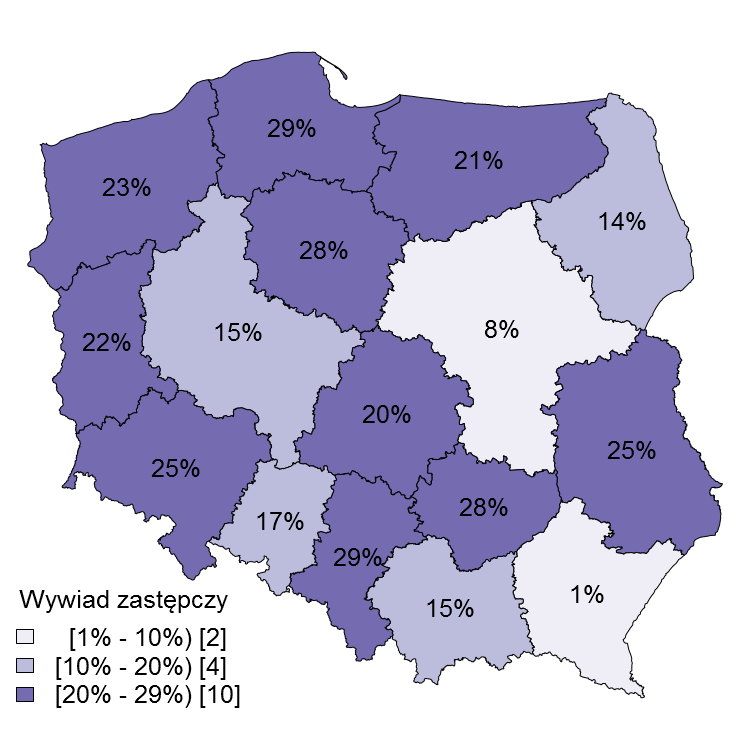
\includegraphics[width=0.6\textwidth]{04_wykresy/wywiad-woj.png}
\caption{Odsetek wywiadów zastępczych w badaniu EU-SILC 2011 w przekroju województw}
\small{Źródło: opracowanie własne na podstawie badania EU-SILC 2011.}
\label{fig:wywiad_woj}
\end{figure}

Rozkład odpowiedzi pochodzących z wywiadu zastępczego charakteryzuje się znacznym przestrzennym zróżnicowaniem (por. rys. \ref{fig:wywiad_woj}). Najwyższy odsetek tak przeprowadzonego wywiadu obserwuje się w województwie pomorskim oraz śląskim --- 29\%. W środkowej grupie z wartościami pomiędzy 14\% a 17\% znalazły się województwa: podlaskie, małopolskie, wielkopolskie oraz opolskie. Województwo mazowieckie charakteryzuje się 8\% udziałem przeprowadzonych wywiadów zastępczych. Z kolei w województwie podkarpackim odnotowano zaledwie 1\% wywiadów zastępczych.

Na rysunku \ref{fig:wywiad_wiek} przedstawiono także występowanie tego zjawiska według roczników wieku.

\begin{figure}[ht]
\centering
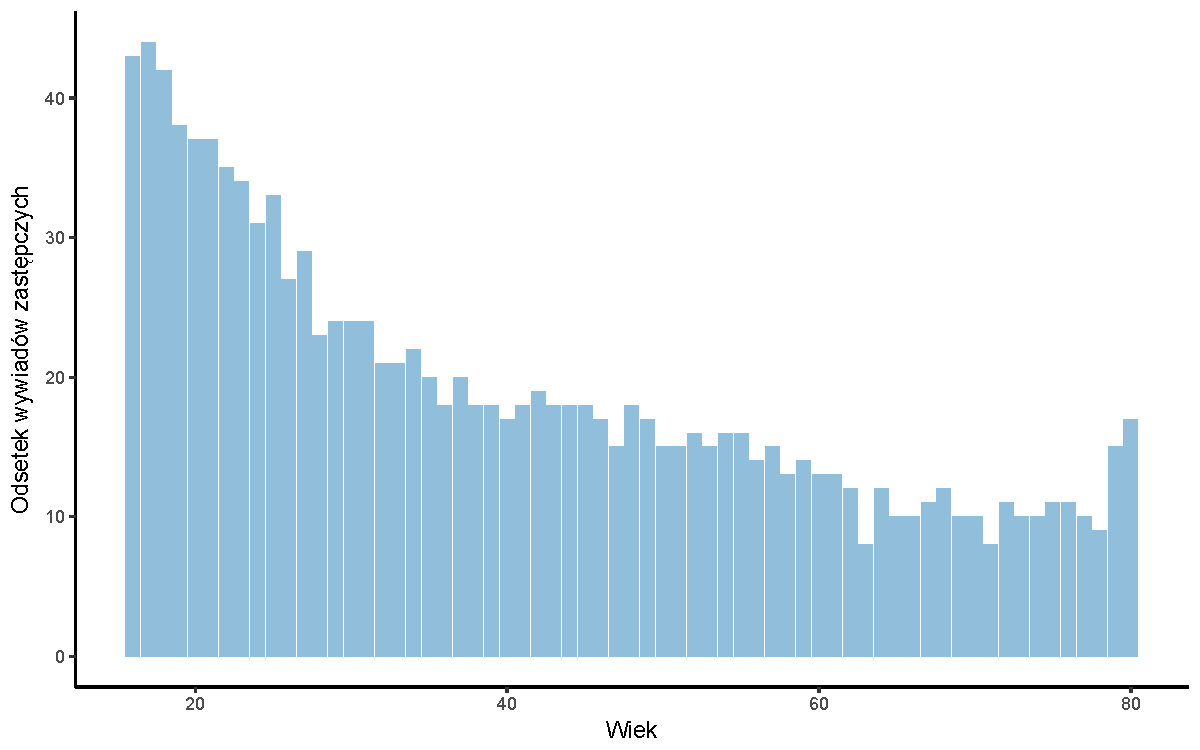
\includegraphics[width=0.8\textwidth]{04_wykresy/sposob_przeprowadzenia_wywiadu_wiek-1.pdf}
\caption{Odsetek wywiadów zastępczych w badaniu EU-SILC według roczników wieku}
\small{Źródło: opracowanie własne na podstawie badania EU-SILC 2011.}
\label{fig:wywiad_wiek}
\end{figure}

Wywiady zastępcze najczęściej były realizowane za osoby w wieku 16, 17 i 18 lat. Można także zaobserwować wyższy udział wywiadów przeprowadzonych w zastępstwie osób w wieku co najmniej 80 lat. Badanie EU-SILC nie wskazuje maksymalnego wieku respondenta, ale w~dostarczonych danych dokonano zgrupowania osób w wieku 80 lat i starszych w~jedną kategorię w~celu zachowania tajemnicy statystycznej \citep{ciani2011}. Niestety, podobnie jak wcześniej, w dokumentacji badania nie ma informacji na ten temat.

\subsection{Analiza struktury cech wykorzystanych w estymacji wskaźników ubóstwa}\label{pr:struktura-zmiennych}

Najistotniejszą z punktu widzenia analizy ubóstwa zmienną jest roczny ekwiwalentny dochód do dyspozycji gospodarstwa. Wyznaczenie tego wektora dochodów polega na zsumowaniu wszystkich składników dochodu gospodarstwa, w tym dochodów poszczególnych osób wchodzących w skład gospodarstwa i pomniejszeniu go o rozchody, czyli przede wszystkim transfery społeczne. Tak wyznaczone wartości przelicza się uwzględniając demograficzny wymiar badanego gospodarstwa z~wykorzystaniem zmodyfikowanej skali ekwiwalentności OECD. Poniżej wymieniono poszczególne składniki składające się na dochód gospodarstwa --- symbol zmiennej w badaniu EU-SILC, pełną nazwę oraz skrót wykorzystywany na rysunkach.

Spośród składników dochodu osób \emph{in plus} wlicza się:

\begin{itemize}
\item PY010G --- dochód pieniężny z pracy najemnej brutto (p.~najemna),
\item PY021G --- wykorzystanie samochodu służbowego do celów prywatnych brutto (samochód),
\item PY050G --- dochód z pracy na własny rachunek brutto (p.~własna),
\item PY080G --- emerytura z indywidualnych funduszy emerytalnych brutto (III filar),
\item PY090G --- świadczenia dla bezrobotnych brutto (św. bezr.),
\item PY100G --- świadczenia związane z wiekiem brutto (św. wiek),
\item PY110G --- renta rodzinna brutto (renta),
\item PY120G --- świadczenia chorobowe brutto (św. chorob.),
\item PY130G --- świadczenia dla niepełnosprawnych brutto (św. niep),
\item PY140G --- stypendia brutto (stypendia).
\end{itemize}

Na poziomie gospodarstwa do dochodu wlicza się:

\begin{itemize}
\item HY040G --- dochód z wynajmu nieruchomości brutto (doch. nieruch.),
\item HY050G --- świadczenia dotyczące rodziny brutto (św. rodz.),
\item HY060G --- świadczenia dotyczące wykluczenia społecznego brutto (św. wykl.),
\item HY070G --- dodatki mieszkaniowe brutto (dod. mieszk.),
\item HY080G --- regularne transfery pieniężne otrzymywane od osób spoza gospodarstwa domowego brutto (transfery),
\item HY090G --- dochód z własności finansowej (kapitałowy) brutto (kapitał),
\item HY110G --- dochód dzieci do lat 16 brutto (doch. dzieci).
\end{itemize}

Na dochód \emph{in minus} wpływają:

\begin{itemize}
\item HY120G --- podatki od nieruchomości brutto (pod. nieruch.),
\item HY130G --- regularne transfery pieniężne przekazywane osobom spoza gospodarstwa domowego brutto (transfery),
\item HY140G --- podatek dochodowy, składki na ubezpieczenie społeczne brutto (pod. doch.).
\end{itemize}

Ponadto każdej zmiennej dochodowej towarzyszy zmienna flagowa, która przechowuje informację o tym czy dana wartość była imputowana i jeśli tak, to w jaki sposób. Według dokumentacji badania, zmienna zawierająca informację o sposobie imputacji powinna być pięciocyfrowa. Wówczas pierwsza cyfra zawiera kategorię dochodu (netto/brutto), druga cyfra to metoda imputacji, natomiast ostatnie trzy cyfry to współczynnik imputacji (iloraz wartości zebranej i zapisanej). W~praktyce poszczególne kraje stosują swoje standardy kodowania tej zmiennej \citep{brandolini2010}. W polskim badaniu EU-SILC na podstawie wartości flagi można wyodrębnić następujące kategorie: 1) kompletna informacja o dochodzie, 2) częściowa informacja o dochodzie oraz 3) brak informacji o dochodzie.

Rysunek \ref{fig:dochod_osoby} przedstawia wartości poszczególnych składników dochodu uzyskiwanych przez osoby zamieszkujące gospodarstwo domowe. Jedna osoba mogła uzyskiwać dochody z kilku źródeł, w związku z czym liczebności wszystkich kategorii nie sumują się do liczby przebadanych respondentów. Z racji bardzo dużych wartości występujących w kategoriach praca najemna oraz praca na własny rachunek ograniczono oś Y do wartości 50 000 zł. 

\begin{figure}[ht]
\centering
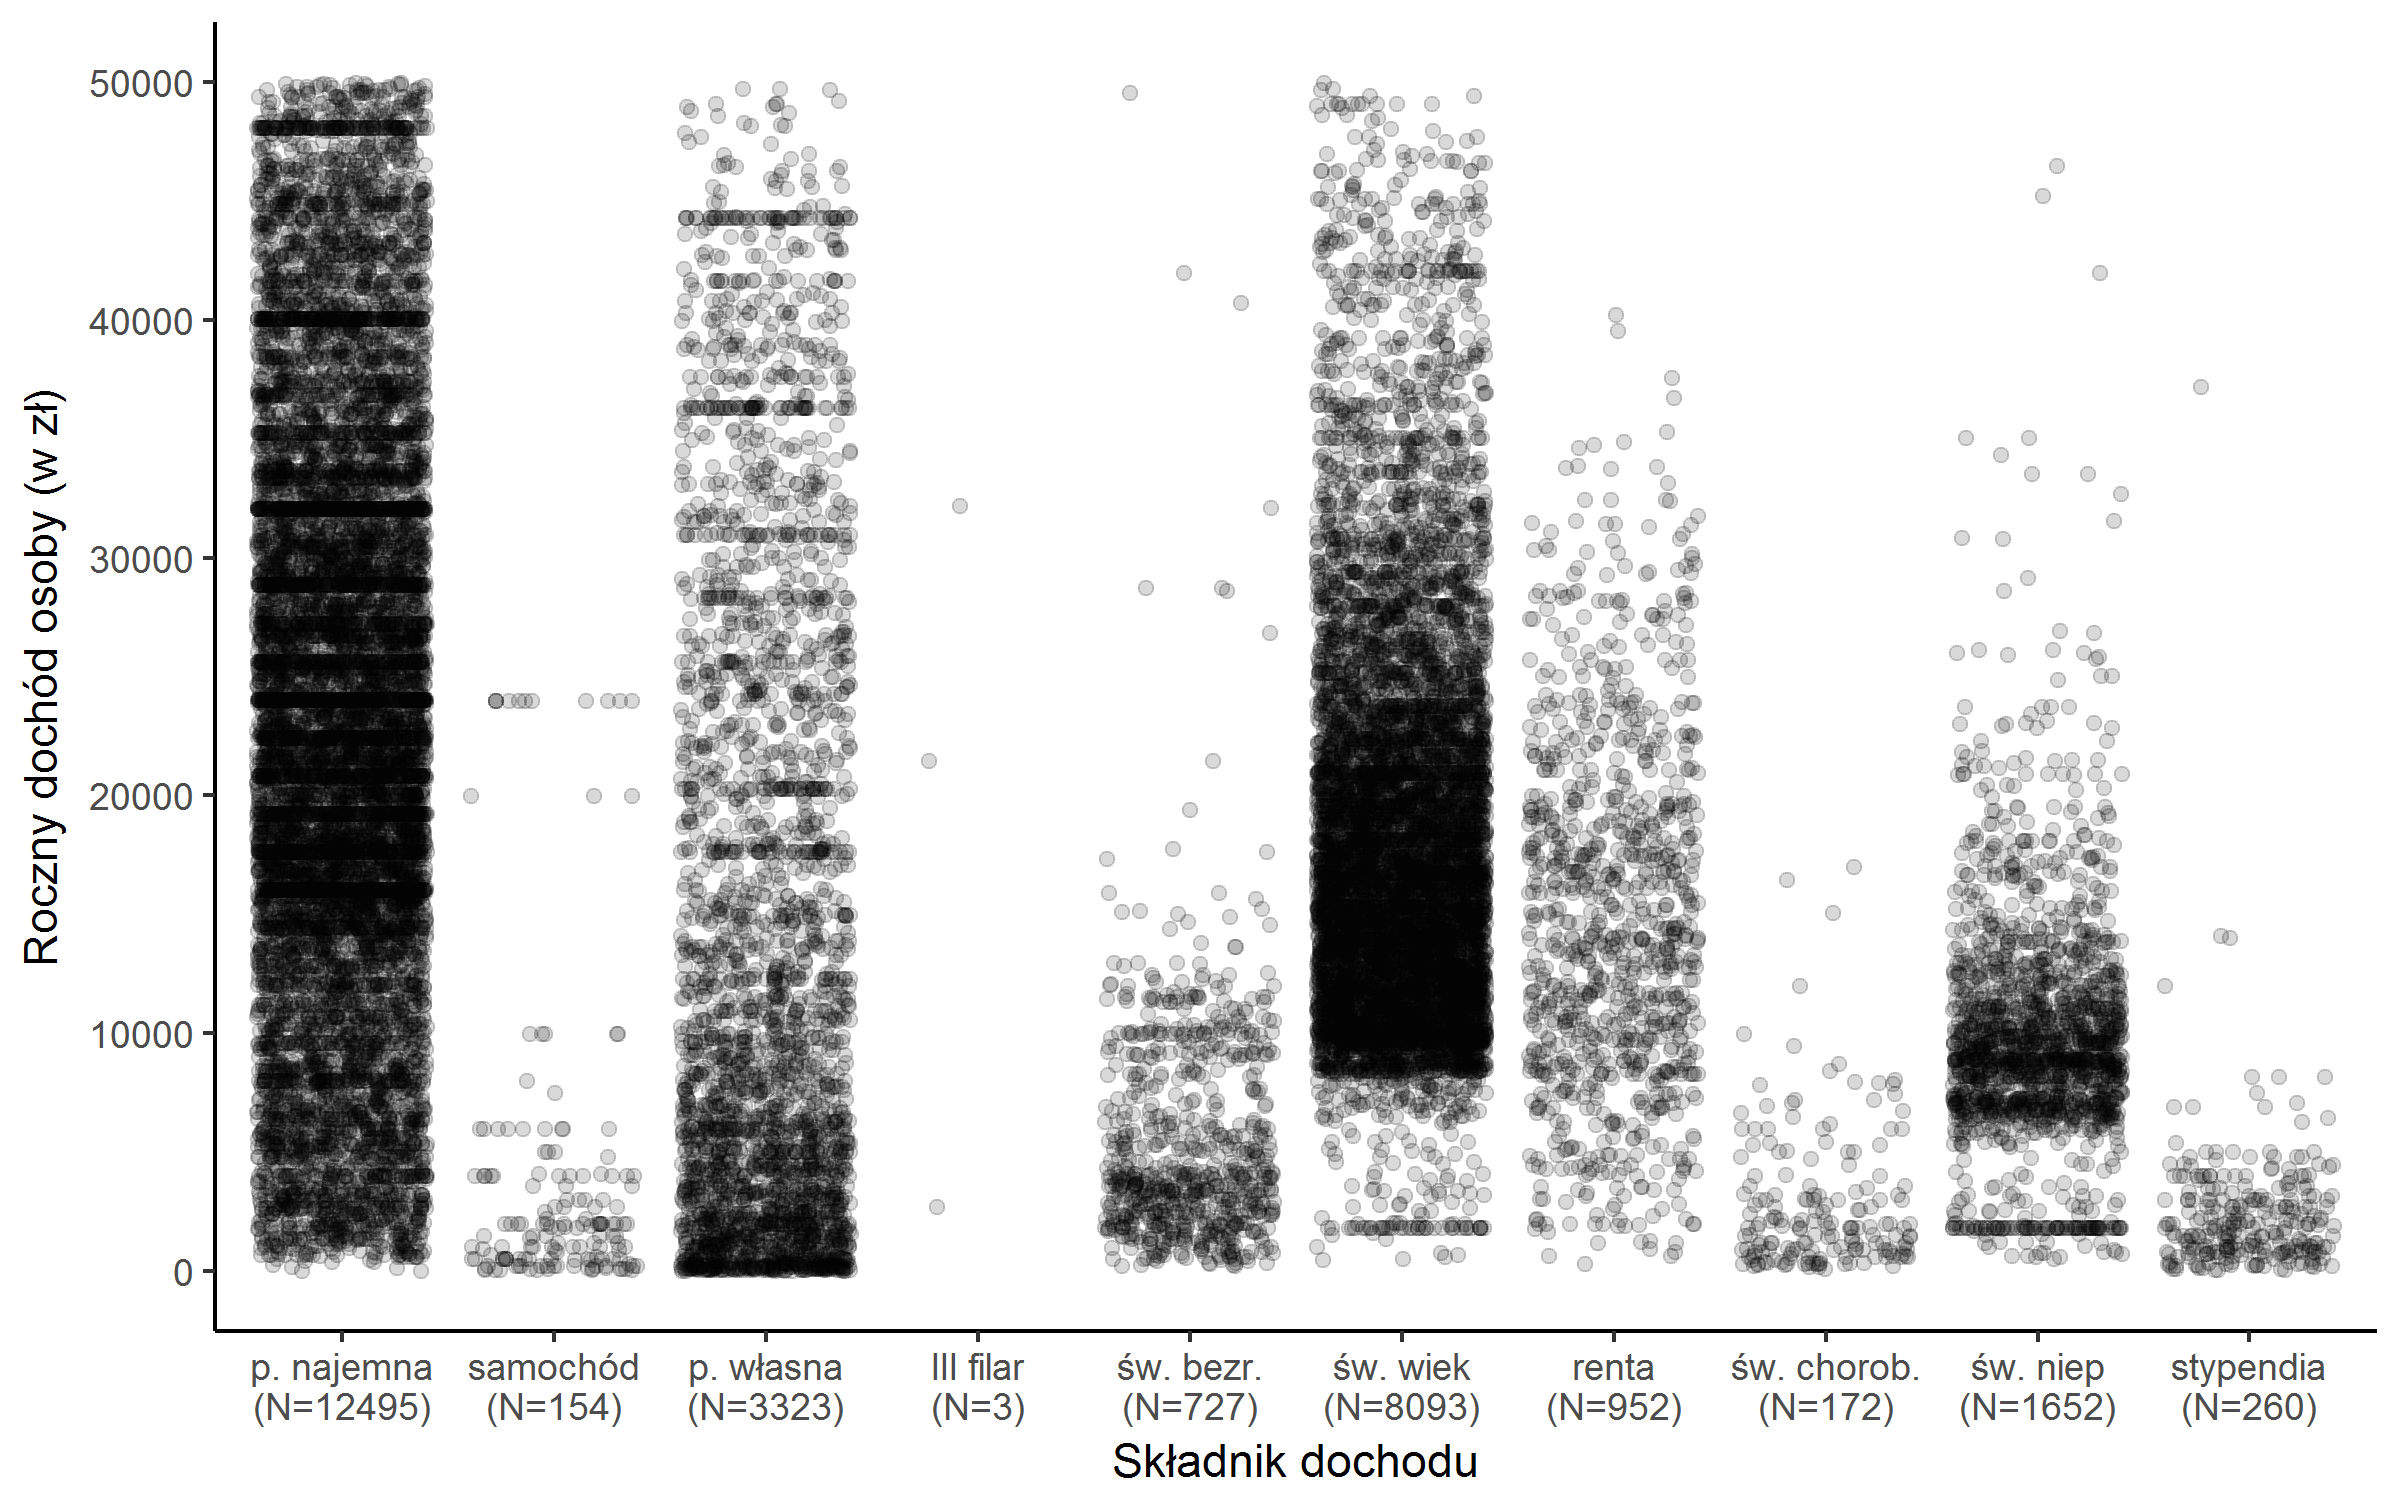
\includegraphics[width=0.8\textwidth]{04_wykresy/dochod_osoby-1.png}
\caption{Wartości dochodu osób w badaniu EU-SILC 2011 według kategorii dochodu (do 50000 zł)}
\small{Źródło: opracowanie własne na podstawie badania EU-SILC 2011.}
\label{fig:dochod_osoby}
\end{figure}

Najczęściej występującą wśród respondentów kategorią dochodu był dochód pieniężny z pracy najemnej (41,1\%). Na kolejnych miejscach znalazły się świadczenia związane z wiekiem (26,6\%) oraz dochód z pracy na własny rachunek (10,9\%). Z kolei najrzadziej wskazywanym źródłem dochodu wśród badanych osób były: emerytura z indywidualnych funduszy emerytalnych (3 osoby), wykorzystanie samochodu służbowego do celów prywatnych (0,5\%) i świadczenia chorobowe (0,6\%).

Najwyższą wartością średnią charakteryzuje się dochód z pracy najemnej (30 861 zł). W tej grupie dochodu występuje także wartość maksymalna --- 651 772 zł. Pod względem wartości średniej na drugim miejscu jest dochód z pracy na własny rachunek brutto (22 527 zł), następnie na bardzo podobnym poziomie znajduje się emerytura z indywidualnych funduszy emerytalnych brutto (18 758 zł) oraz świadczenia związane z wiekiem brutto (18 703 zł). Największą dyspersją cechują się kategorie: wykorzystanie samochodu służbowego do celów prywatnych brutto (155,3\%) oraz dochód z pracy na własny rachunek brutto (138,2\%). Najmniejsze zróżnicowanie cechy obserwuje się w trzech kategoriach dochodu: świadczenia związane z wiekiem brutto (48,9\%), świadczenia dla niepełnosprawnych brutto (49,7\%) oraz renta rodzinna brutto (51,4\%).

Rysunek \ref{fig:dochod_osoby} pozwala określić, które wartości pojawiają się najczęściej w poszczególnych kategoriach. Na szczególną uwagę zasługują kategorie: świadczenia związane z wiekiem i dla niepełnosprawnych, w których widoczna jest liczna grupa jednostek, dla których wartość cechy wynosi dokładnie 1 834 zł. Ponadto występowanie podobnych wartości wskazuje na skłonność respondentów do zaokrąglania podawanych kwot. Można także zauważyć, że wartości w kategoriach praca najemna, praca na własny rachunek czy stypendia mają dolną granicę w okolicy zera. Z~kolei świadczenia (z wyłączeniem zasiłków dla bezrobotnych oraz chorobowych) wyraźną dolną granicę mają na poziomie około 10 000 zł.

Rysunek \ref{fig:dochod_osoby_imp} przedstawia udział imputowanych wartości w poszczególnych składnikach dochodowych.

\begin{figure}[ht]
\centering
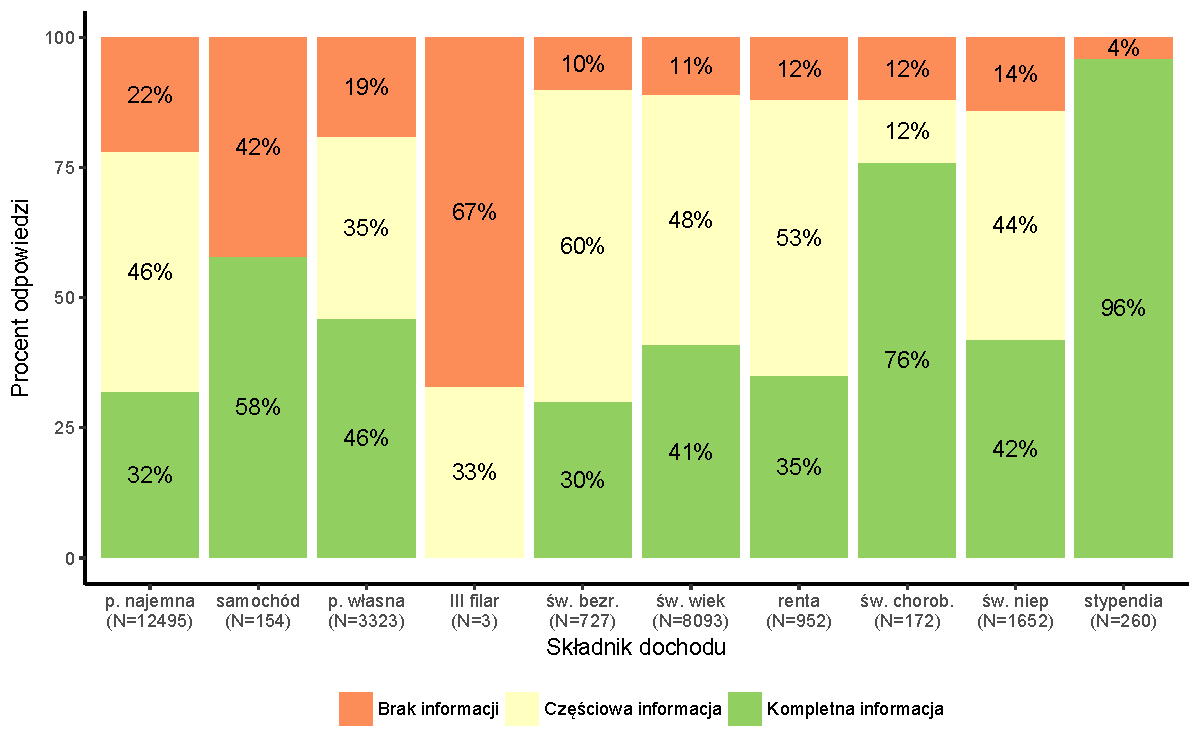
\includegraphics[width=0.8\textwidth]{04_wykresy/dochod_osoby_imputacja-1.pdf}
\caption{Odsetek imputowanych wartości dochodu w badaniu EU-SILC 2011 według kategorii dochodu}
\small{Źródło: opracowanie własne na podstawie badania EU-SILC 2011.}
\label{fig:dochod_osoby_imp}
\end{figure}

W większości przypadków odsetek braku informacji, a co za tym idzie całkowita imputacja wartości, nie przekraczał 22\% wszystkich odpowiedzi w ramach każdej z wyróżnionych kategorii. Wyjątkiem jest tu cecha: wykorzystanie samochodu służbowego do celów prywatnych brutto, gdzie brak informacji stanowił 42\%. Największy odsetkiem kompletnych danych charakteryzuje się cecha stypendia brutto --- 96\%.	

Następnie analizie poddano zależność pomiędzy sposobem odpowiedzi, a odsetkiem imputowanych wartości. Rysunek \ref{fig:dochod_osoby_imp_prox} przedstawia zestawienie struktury imputacji poszczególnych kategorii dochodu i struktury metody pozyskania odpowiedzi. Przy nazwach cech podano liczebności poszczególnych kategorii.

\begin{figure}[ht]
\centering
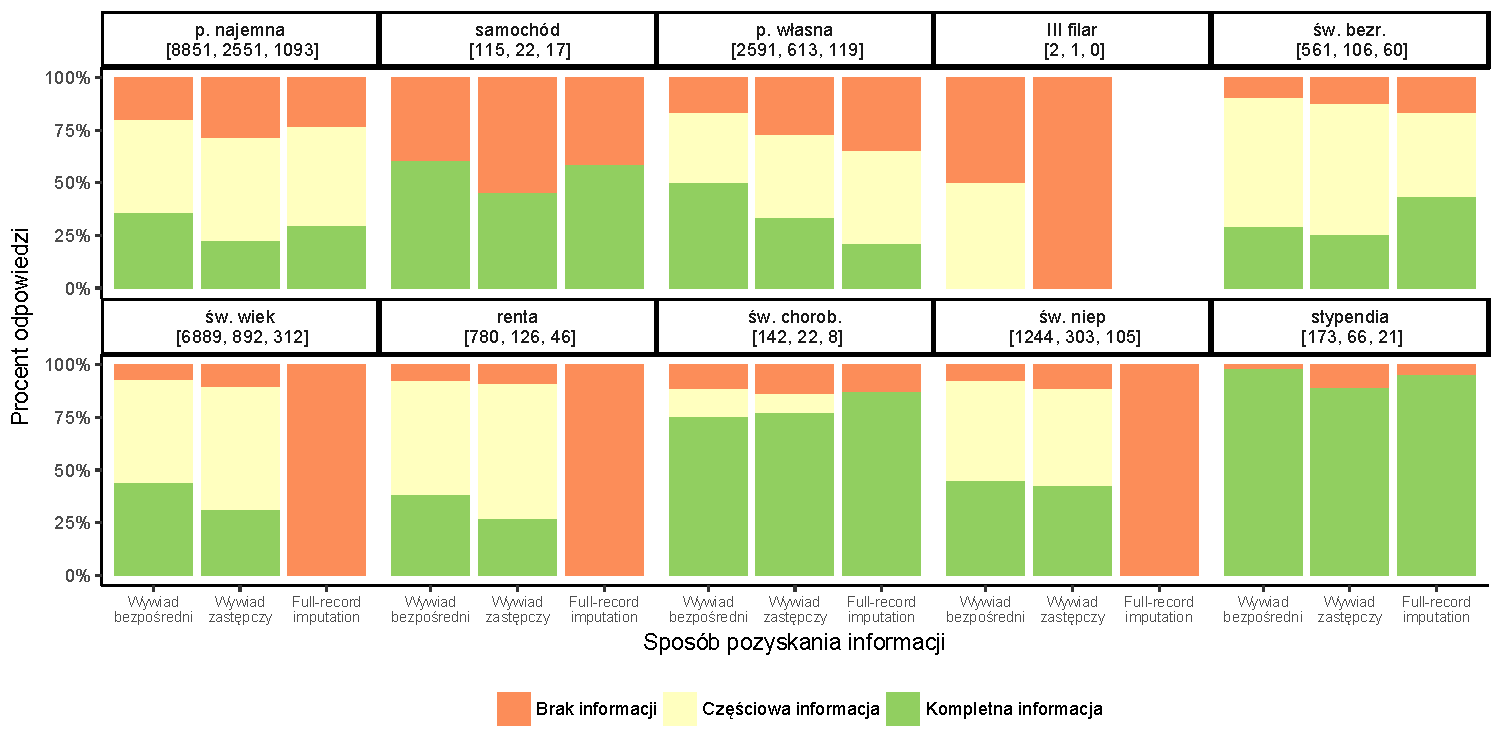
\includegraphics[width=0.8\textwidth]{04_wykresy/dochod_osoby_imputacja_proxy-1.pdf}
\caption{Odsetek imputowanych wartości dochodu w badaniu EU-SILC 2011 według kategorii dochodu oraz sposobu odpowiedzi}
\small{Źródło: opracowanie własne na podstawie badania EU-SILC 2011.}
\label{fig:dochod_osoby_imp_prox}
\end{figure}

We wszystkich kategoriach dochodu obserwowana jest większa frakcja wartości imputowanych w przypadku, gdy był przeprowadzany wywiad zastępczy. Mniejszy jest natomiast odsetek jednostek, dla których uzyskano kompletną informację o dochodzie. Należy jednak podkreślić to, że analizowane grupy były różnoliczne.

Rysunek \ref{fig:dochod_gosp} prezentuje dane dotyczące dochodów na poziomie gospodarstwa domowego. Także w tym przypadku z racji występowania obserwacji o bardzo dużych wartościach cechy w kategorii dochód z własności finansowej ograniczono oś Y do wartości 50 000 zł.

\begin{figure}[ht]
\centering
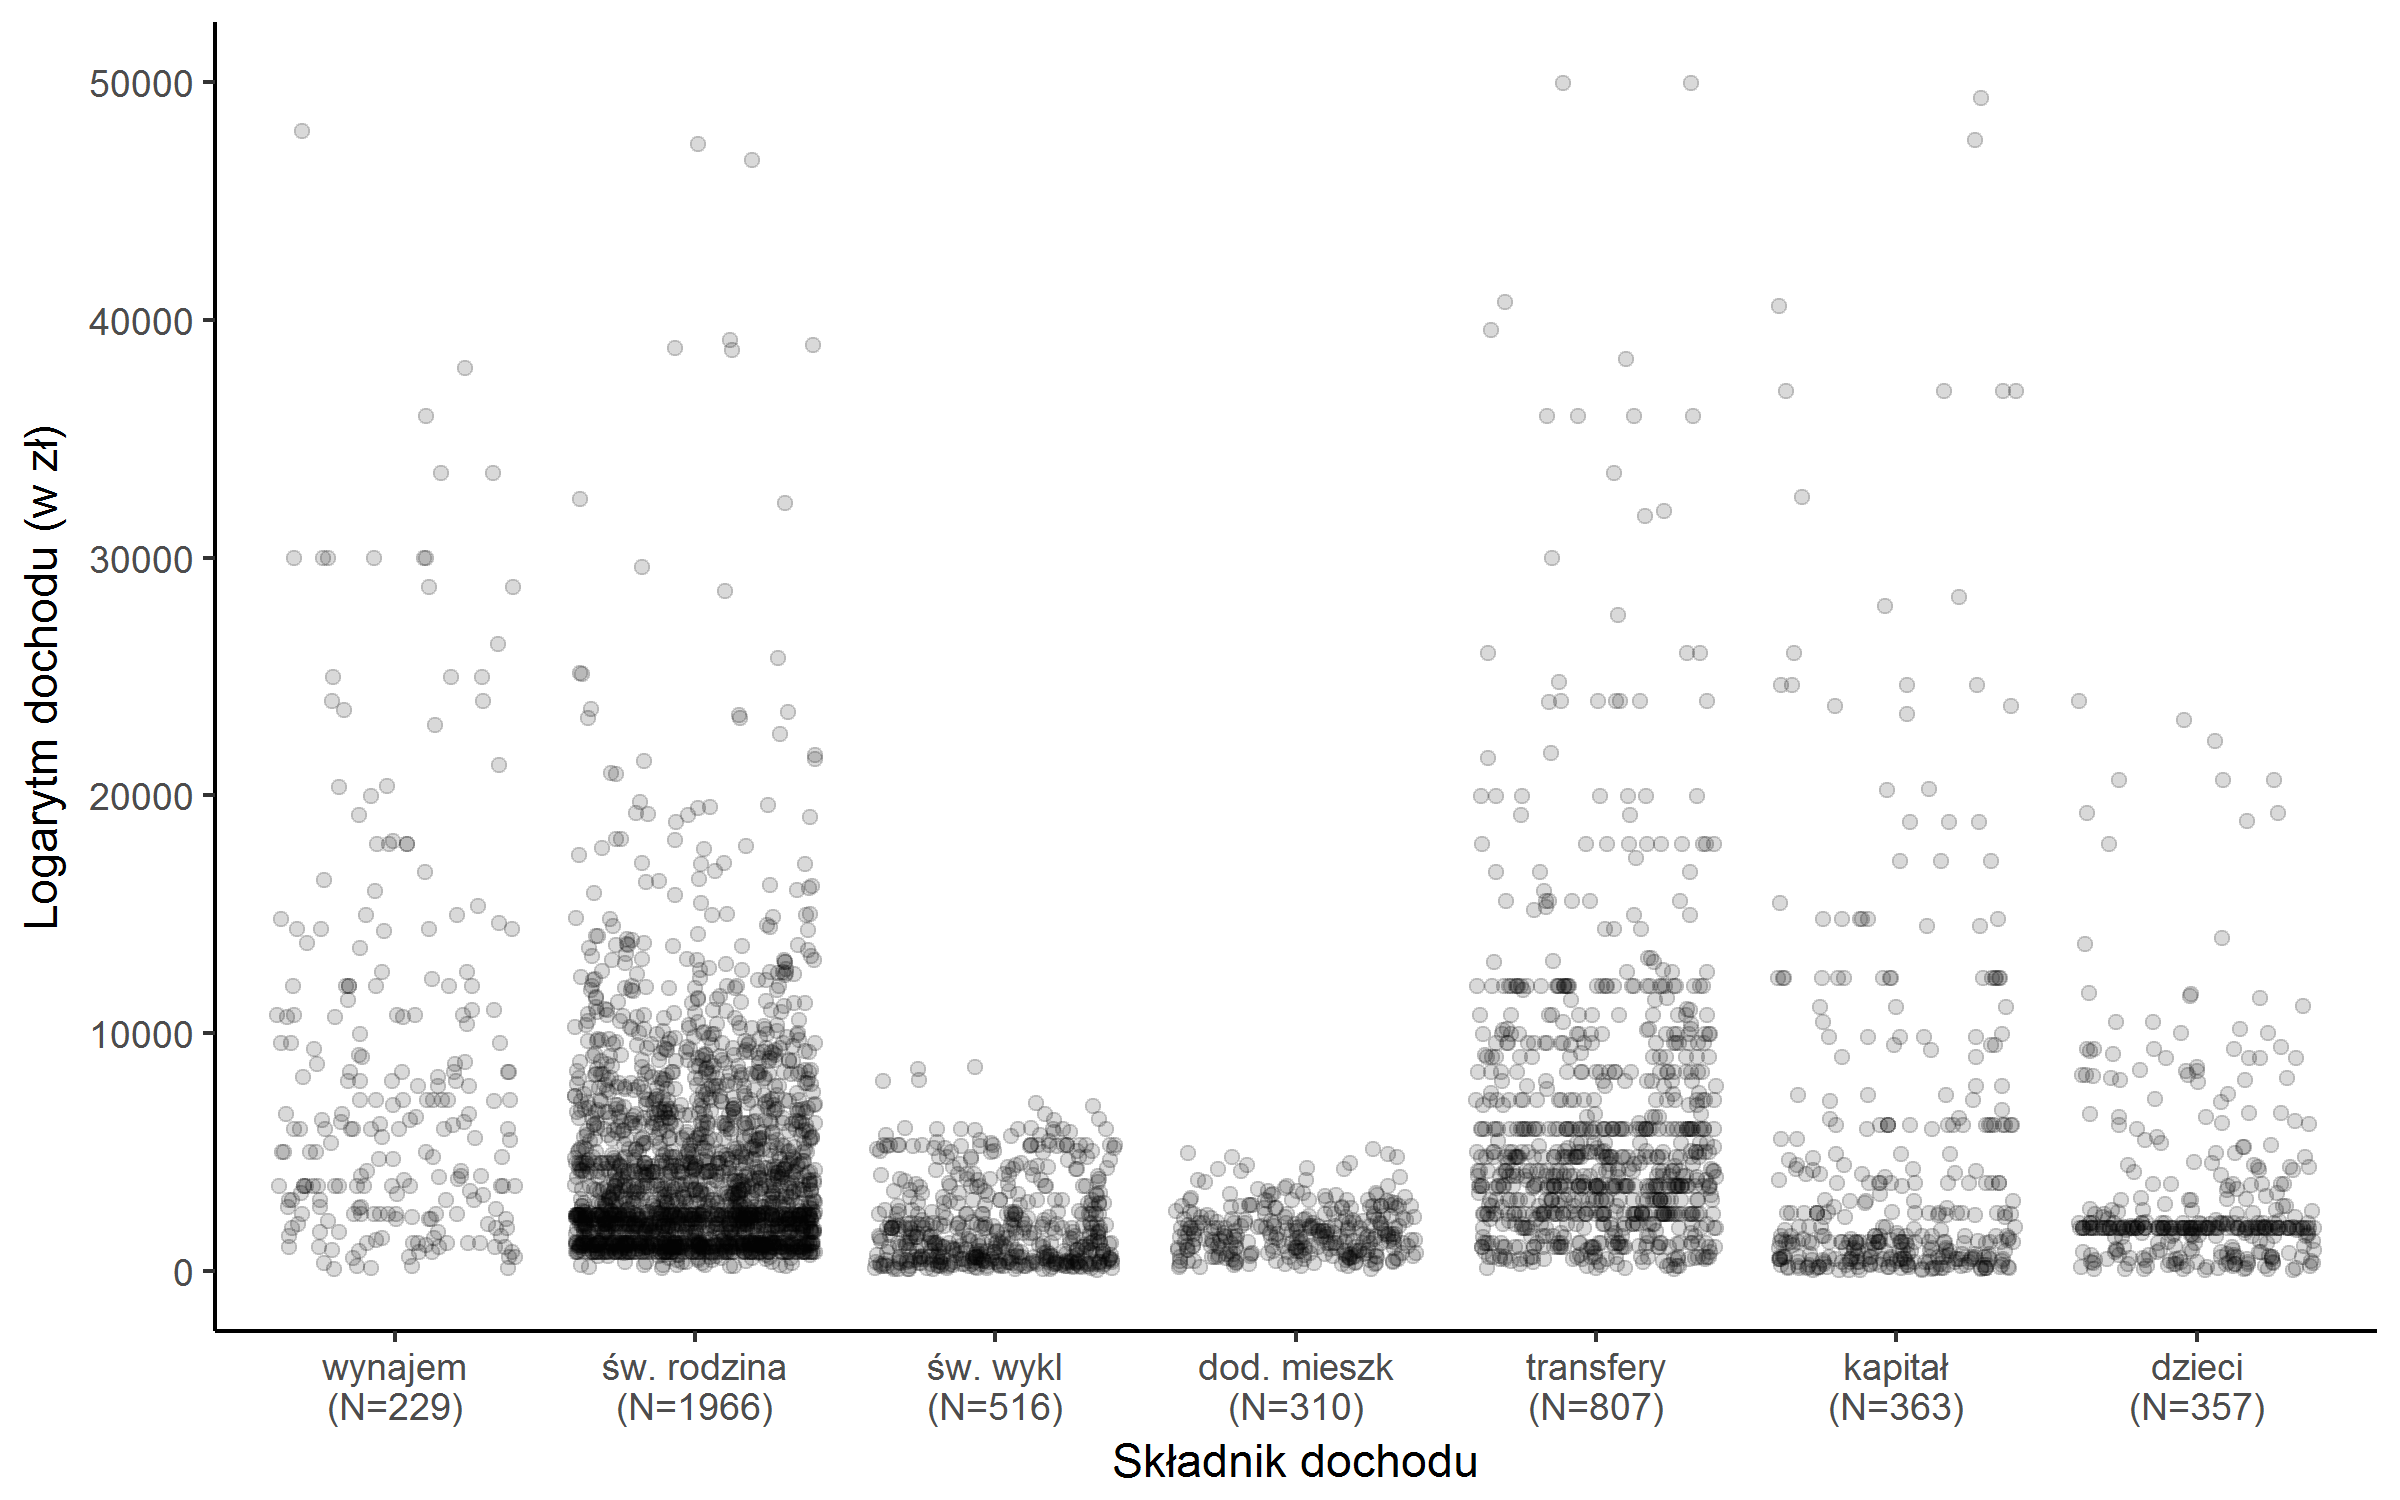
\includegraphics[width=0.8\textwidth]{04_wykresy/dochod_gospodarstw-1.png}
\caption{Wartości dochodu gospodarstw w badaniu EU-SILC 2011 według kategorii dochodu (do 50000 zł)}
\small{Źródło: opracowanie własne na podstawie badania EU-SILC 2011.}
\label{fig:dochod_gosp}
\end{figure}

W tym przypadku najczęściej występującą kategorią dochodu są świadczenia dotyczące rodziny (15,3\%) oraz regularne transfery pieniężne otrzymywane od osób spoza gospodarstwa domowego (6,3\%). Najrzadziej gospodarstwa deklarowały dochody pochodzące z wynajmu nieruchomości (1,8\%) oraz dodatków mieszkaniowych (2,4\%). Najwyższa wartość średnia występuje w kategorii dochód z własności finansowej (kapitałowy) brutto (15 443 zł). Ta sama kategoria cechuje się także wartością maksymalną (799 059 zł) oraz największym zróżnicowaniem (484,2\%).

W ramach najliczniejszej kategorii dochodu czyli świadczeń dotyczących rodziny występuje bardzo liczna grupa jednostek, dla których wartość cechy wynosi 815 zł. Także w przypadku dochodu dzieci do lat 16 obserwuje się liczne obserwacje, dla których cecha przyjmuje wartość równą 1 834 zł.

W ramach prowadzonej analizy wyznaczono także udział imputowanych wartości w poszczególnych kategoriach dochodu --- rysunek \ref{fig:dochod_gosp_imp}.

\begin{figure}[htp]
\centering
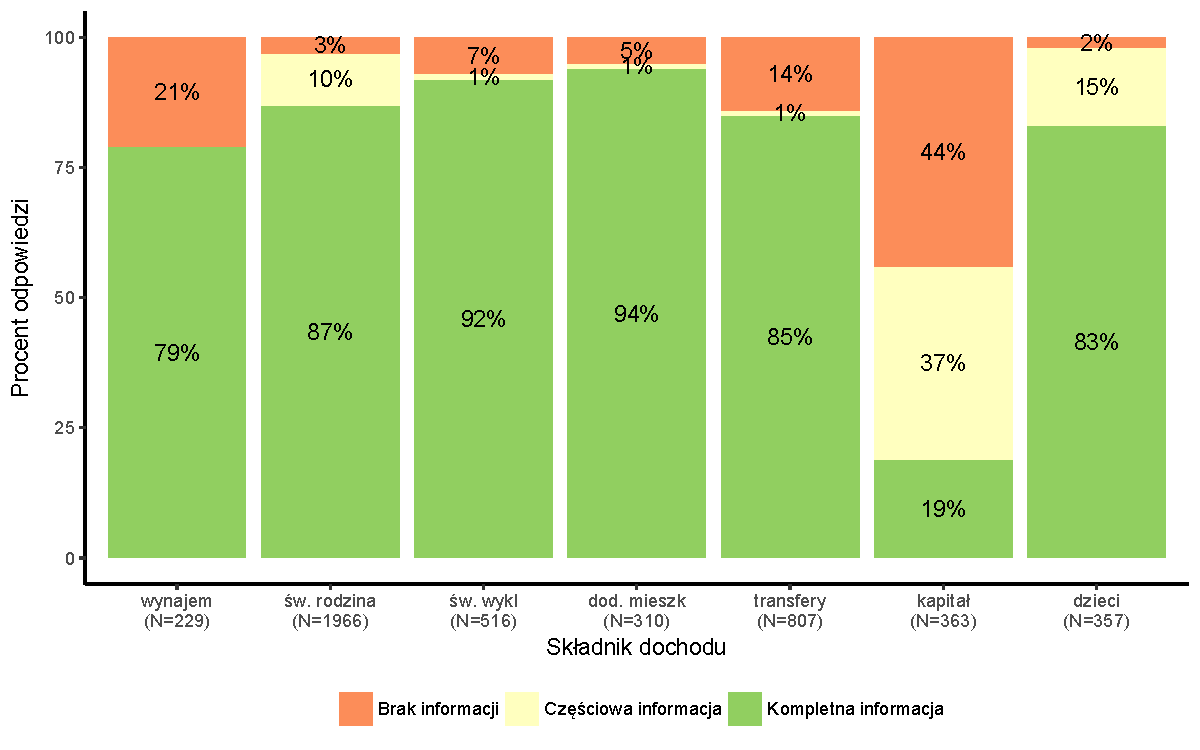
\includegraphics[width=0.8\textwidth]{04_wykresy/dochod_gospodarstw_imputacja-1.pdf}
\caption{Odsetek imputowanych wartości dochodu gospodarstw w badaniu EU-SILC 2011 według kategorii dochodu}
\small{Źródło: opracowanie własne na podstawie badania EU-SILC 2011.}
\label{fig:dochod_gosp_imp}
\end{figure}

W przypadku dochodu zbieranego na poziomie gospodarstwa większość informacji była kompletna. Wyjątkiem jest kategoria dochodu określająca dochód z własności finansowej (kapitałowej) brutto --- brak informacji stanowił tu 44\%, zaś częściową informację o dochodzie uzyskano w przypadku 37\% badanych jednostek.

Informacja na temat sposobu przeprowadzenia wywiadu jest przypisywana do konkretnej osoby w gospodarstwie, w związku z czym analiza zależności pomiędzy imputacją a przeprowadzeniem wywiadu na poziomie gospodarstwa nie była możliwa do przeprowadzenia.

Dalszą część analizy poświecono rozchodom. Na rysunku \ref{fig:trans_spol} przedstawiono rozkład transferów społecznych, które wpływają \emph{in minus} na dochód gospodarstwa domowego.

\begin{figure}[htp]
\centering
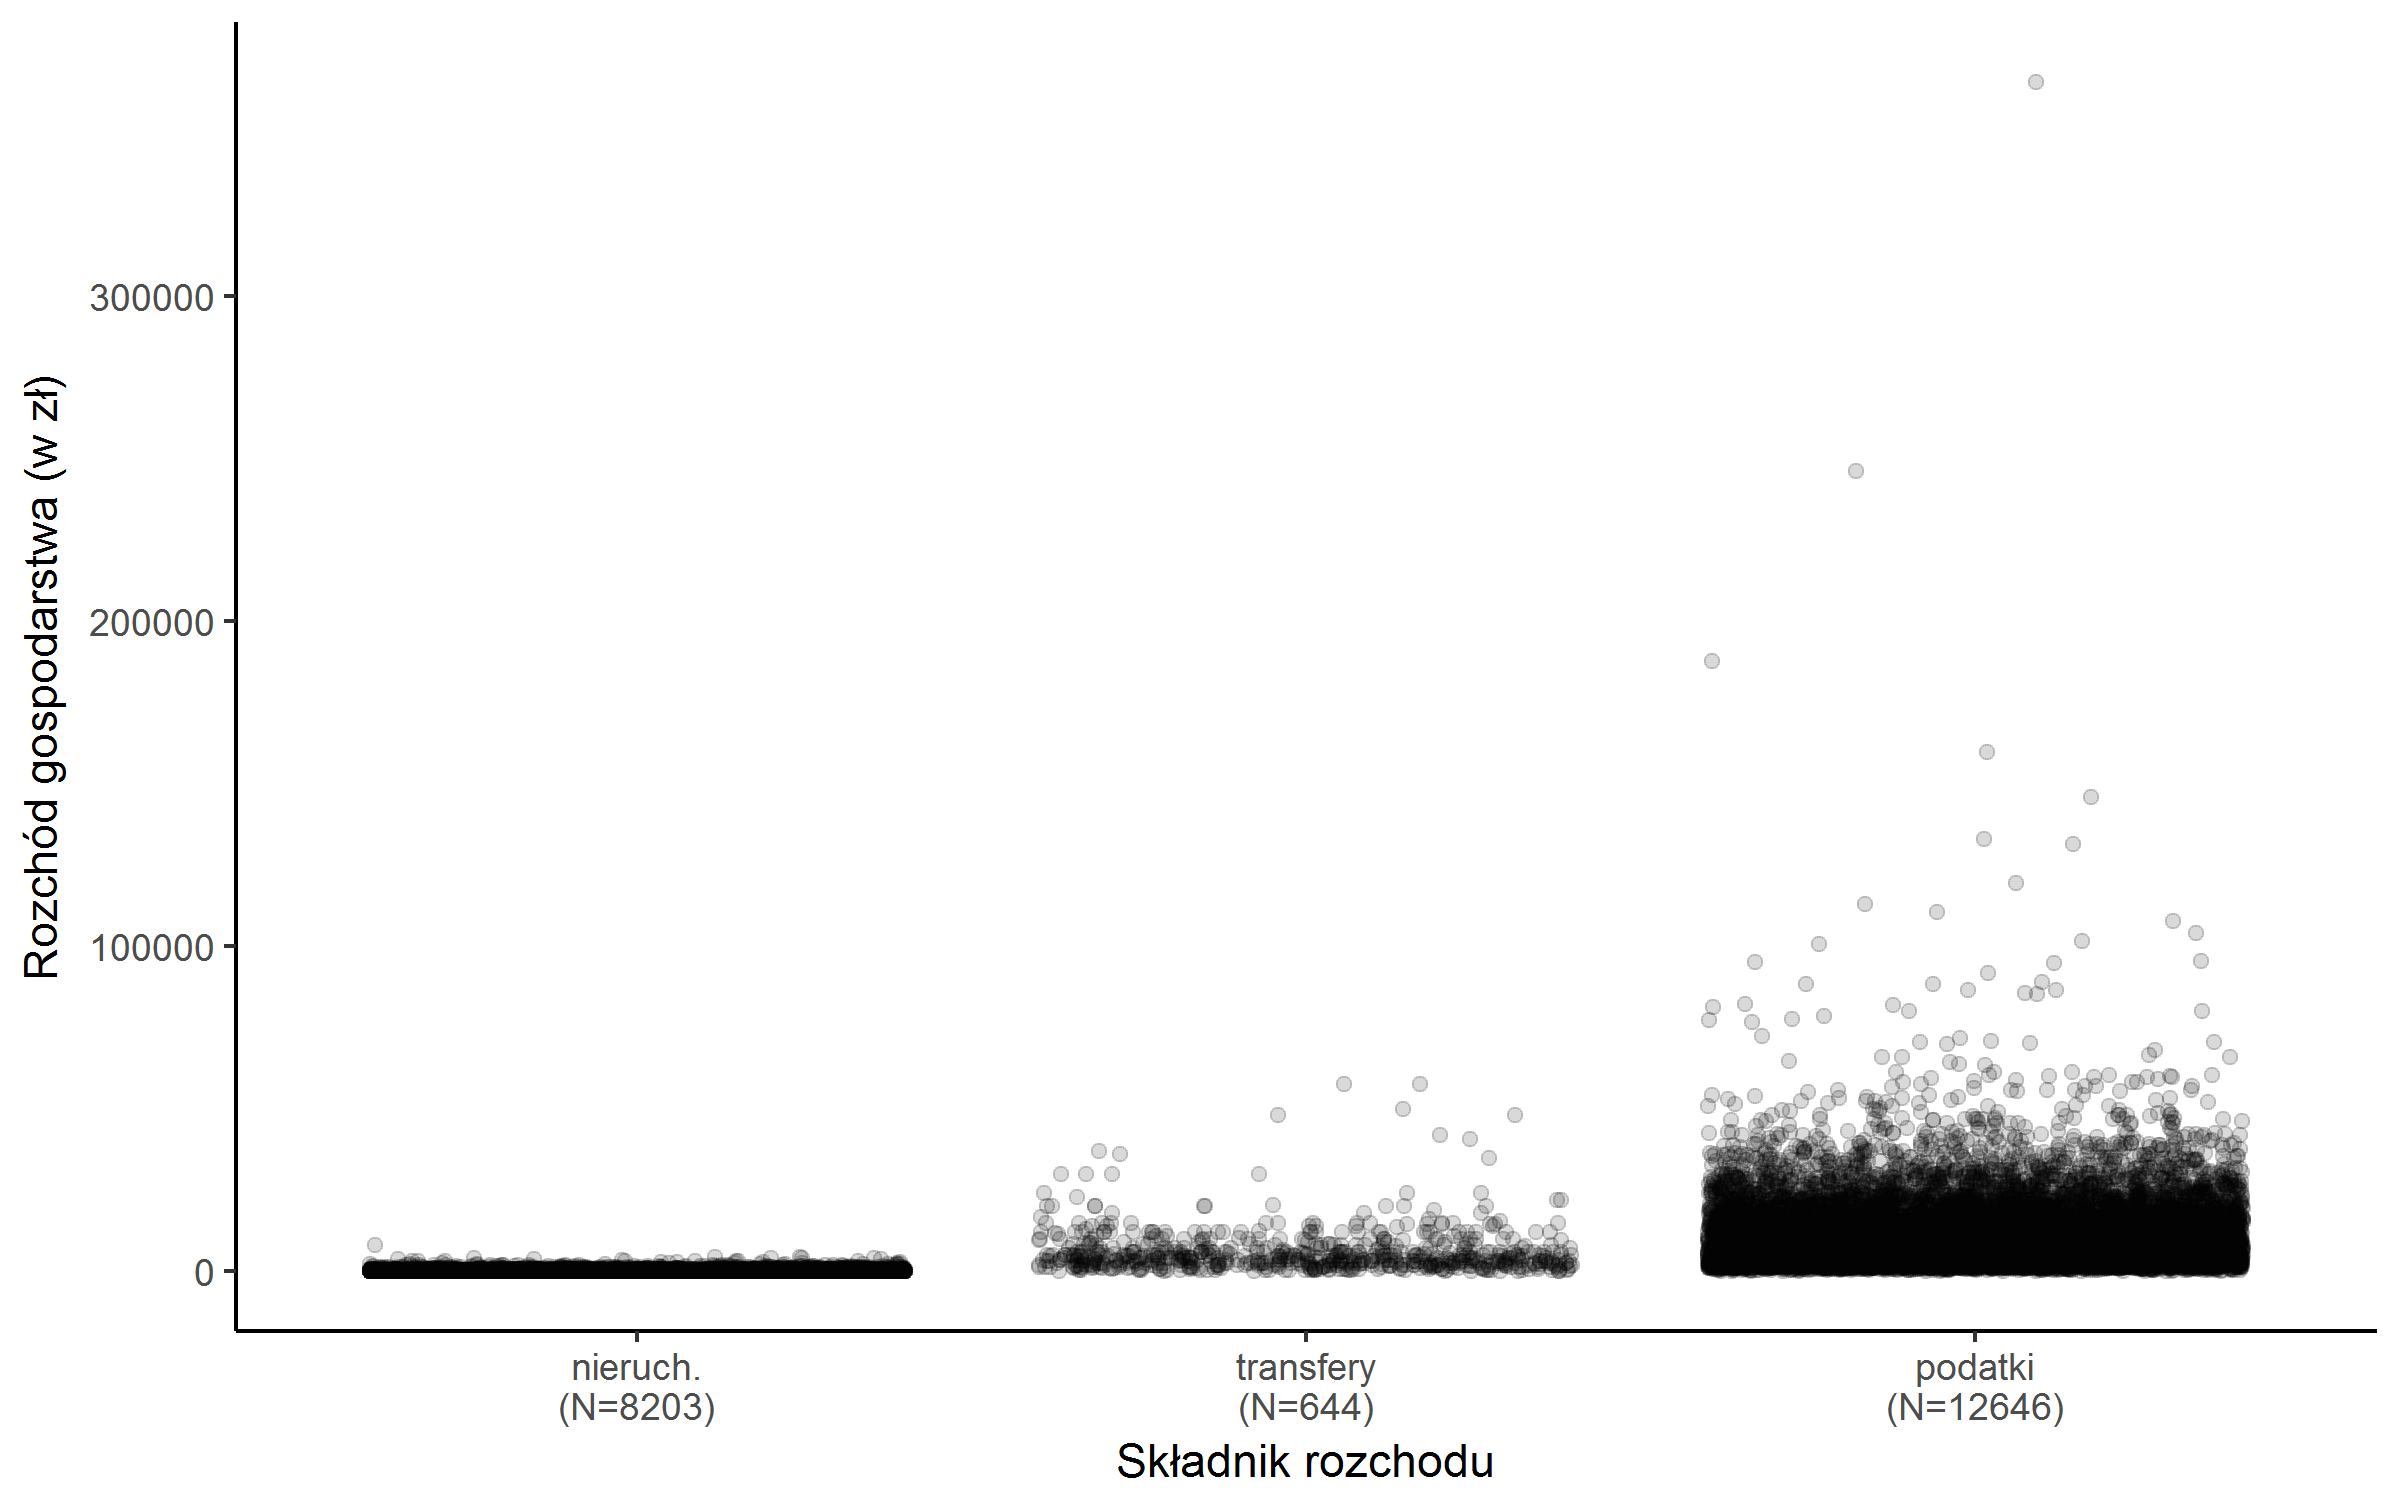
\includegraphics[width=0.8\textwidth]{04_wykresy/transfery_spoleczne-1.png}
\caption{Wartości transferów społecznych gospodarstw w badaniu EU-SILC 2011 według kategorii rozchodu}
\small{Źródło: opracowanie własne na podstawie badania EU-SILC 2011.}
\label{fig:trans_spol}
\end{figure}

Blisko 99\% badanych gospodarstw wykazało w swoich obciążeniach podatek dochodowy oraz składki na ubezpieczenie społeczne. Na drugim miejscu pod względem częstości znalazły się podatki od nieruchomości (63,7\%). Niewielki odsetek respondentów (5\%) wykazał regularne transfery pieniężne przekazywane osobom spoza gospodarstwa domowego. Najwyższa obserwowana wartość podatku odprowadzona przez gospodarstwo domowe wynosiła 365 822 zł.

W następnej kolejności wyznaczono frakcje poszczególnych sposobów imputacji (por. rysunek \ref{fig:trans_spol_imp}).

\begin{figure}[htp]
\centering
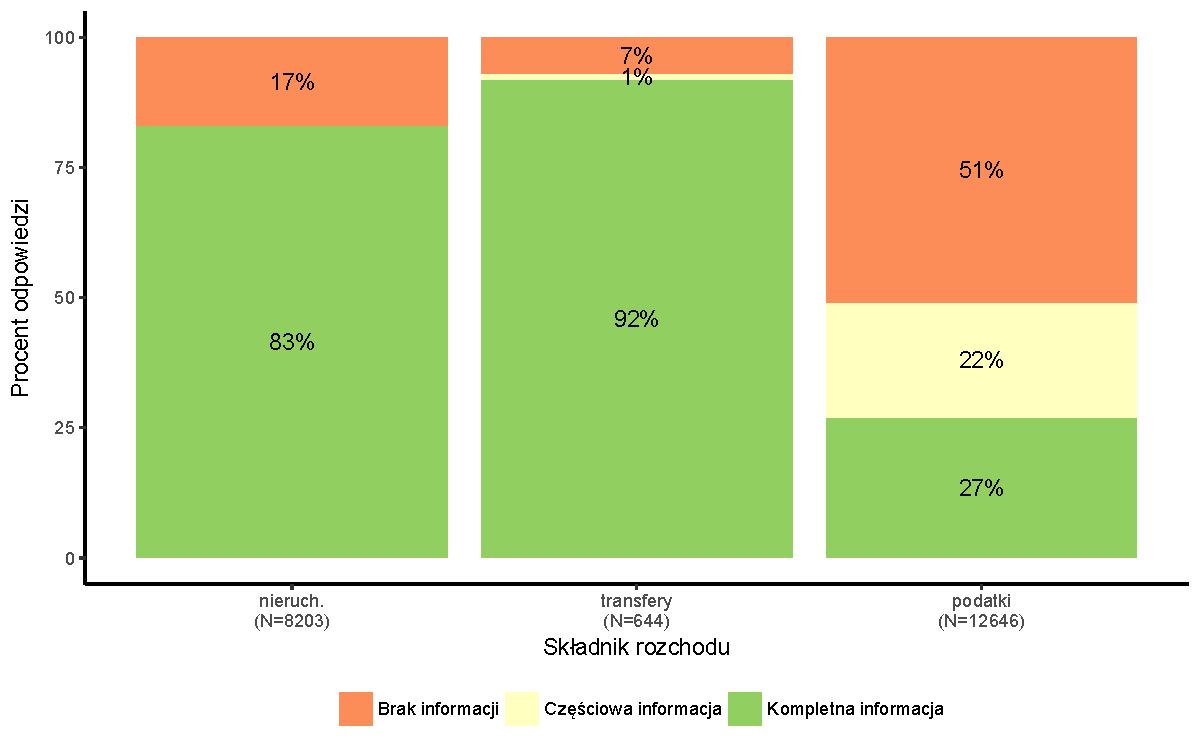
\includegraphics[width=0.8\textwidth]{04_wykresy/tranfery_spoleczne_imputacja-1.pdf}
\caption{Odsetek imputowanych wartości transferów społecznych w badaniu EU-SILC 2011 według kategorii rozchodu}
\small{Źródło: opracowanie własne na podstawie badania EU-SILC 2011.}
\label{fig:trans_spol_imp}
\end{figure}

W kategorii rozchodów największym zróżnicowaniem pod względem kompletności cechuje się podatek dochodowy, składki na ubezpieczenie społeczne brutto. Tylko 27\% respondentów przekazało na ten temat kompletną informację, natomiast dla 51\% jednostek wartość cechy musiała być całkowicie imputowana.

%\subsection{Dochód ekwiwalentny}

Na podstawie kategorii dochodów i rozchodów przedstawionych na początku niniejszego rozdziału, uzyskano wektor dochodów uwzględniający transfery społeczne. W analizach ekonomicznych dochód zwykle przelicza się uwzględniając wymiar demograficzny gospodarstwa domowego. Najprostszym tego typu przekształceniem jest obliczenie dochodu przypadającego na 1 osobę w~gospodarstwie. Takie podejście ma jednak wadę polegającą na nieuwzględnieniu zróżnicowania potrzeb osób w gospodarstwie wynikających z jego wielkości oraz wieku jego członków. Zastosowanie odpowiedniej skali ekwiwalentności umożliwia uwzględnienie tych różnic. Wykorzystując wzór na zmodyfikowaną skalę ekwiwalentności OECD i bazując na danych dotyczących liczby osób w wieku co najmniej 14 lat oraz poniżej tego wieku wyznaczono współczynniki ekwiwalentności. Na tej podstawie w analizowanym zbiorze danych zidentyfikowano 51 typów gospodarstw o różnych składach demograficznych. 

Najliczniej reprezentowaną grupą gospodarstw są gospodarstwa zamieszkiwane przez dwie osoby powyżej 14 roku życia. 73 procent wszystkich gospodarstw domowych stanowią gospodarstwa, w których nie występuje żadna osoba poniżej 14 roku życia. Ponadto w próbie znalazły się także gospodarstwa o bardzo dużej liczbie członków --- największe z nich składało się z 17 osób, w tym 4 osób poniżej 14 roku życia.

Uwzględniając skład demograficzny gospodarstwa wyznaczono wektor dochodów ekwiwalentnych, który stał się podstawą dalszych analiz. 

% Rozkład tego dochodu przedstawiony jest na rysunku \ref{fig:doch_ekw}.

% \begin{figure}[htp]
% 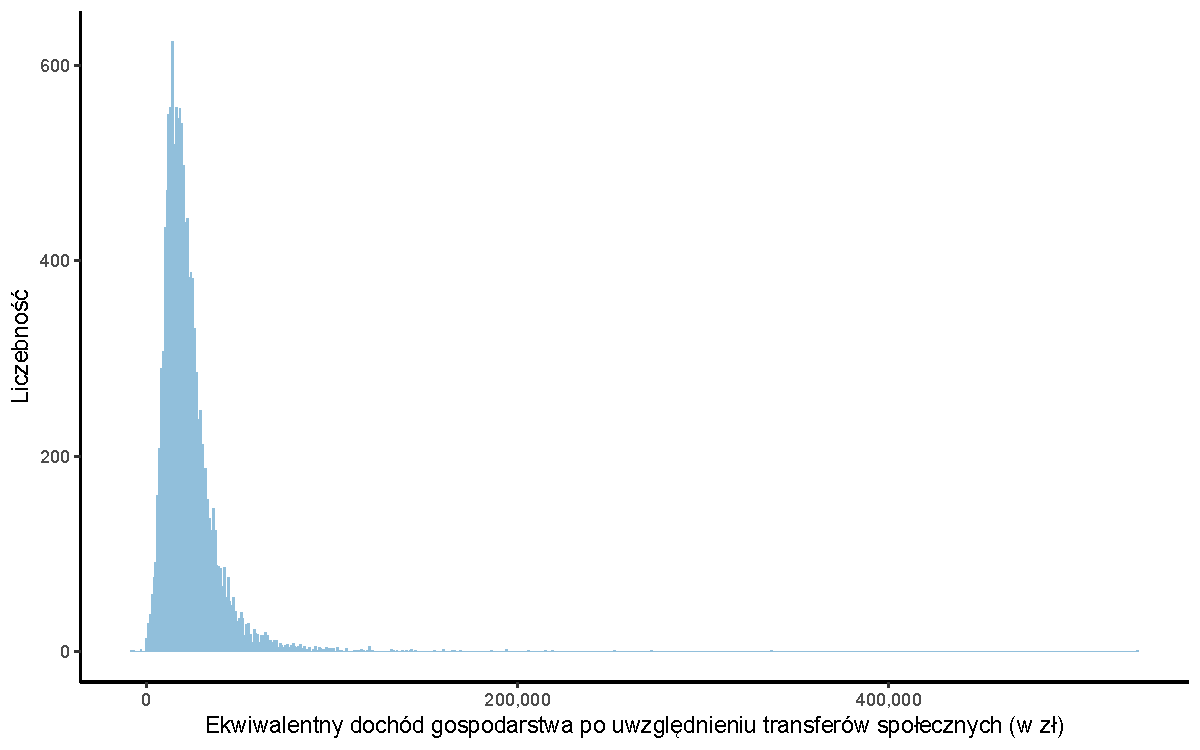
\includegraphics[width=\textwidth]{04_wykresy/dochod_ekiwalentny-1.pdf}
% \caption{Rozkład dochodu ekiwalentnego w badaniu EU-SILC 2011}
% \small{Źródło: opracowanie własne na podstawie badania EU-SILC 2011.}
% \label{fig:doch_ekw}
% \end{figure}

Średni dochód ekwiwalentny wyniósł 22 453 zł, natomiast mediana 19 130 zł. Rozkład dochodów gospodarstw domowych charakteryzował się bardzo dużym zróżnicowaniem --- współczynnik zmienności wynosił 71\%. Znaną powszechnie własnością rozkładu dochodu jest jego silna asymetria prawostronna --- w tym przypadku trzeci moment centralny był równy 6,23. W badaniu EU-SILC 2011 znalazło się 14 gospodarstw, których dochody były ujemne. Minimalna wartość dochodu wynosiła -7 800 zł. Z kolei w siedmiu gospodarstwach domowych dochód ekwiwalentny przekraczał 200 tys. złotych. Gospodarstwa te znajdowały się w powiatach: krapkowickim (województwo opolskie), m. Gdańsk, złotoryjski (dolnośląskie), m. st. Warszawa, m. Lublin (lubelskie). Maksymalna wartość rocznego dochodu ekwiwalentnego wynosiła 534 337 zł (powiat krapkowicki).

\section{Analiza próby}

Pierwszym etapem w estymacji dla małych domen jest analiza liczebności próby oraz określenie liczby reprezentantów posiadających badaną cechę (fakt przynależności do sfery ubóstwa).

\subsection{Liczebność próby i reprezentantów}

Z punktu widzenia estymacji dla małych obszarów bardzo ważne zagadnienie stanowi liczebność całej próby oraz liczba jednostek --- reprezentantów posiadających określony wariant badanej cechy. W przypadku analizy ubóstwa tą cechą będzie przynależność do sfery niedostatku. Dana domena może być licznie reprezentowana w próbie, a mimo to estymacja będzie niemożliwa z~powodu braku ubogich jednostek. W niniejszej analizie za granicę ubóstwa przyjęto 60\% mediany dochodów ekwiwalentnych, która w 2011 roku wynosiła 12 045 zł (por. podrozdział \ref{pr:identyfikacja-ubostwa}).

Na rysunku \ref{fig:proba_reprez} zestawiono liczebność próby oraz reprezentantów w nieplanowanych domenach tj. podregionach i powiatach.

\begin{figure}[htp]
\centering
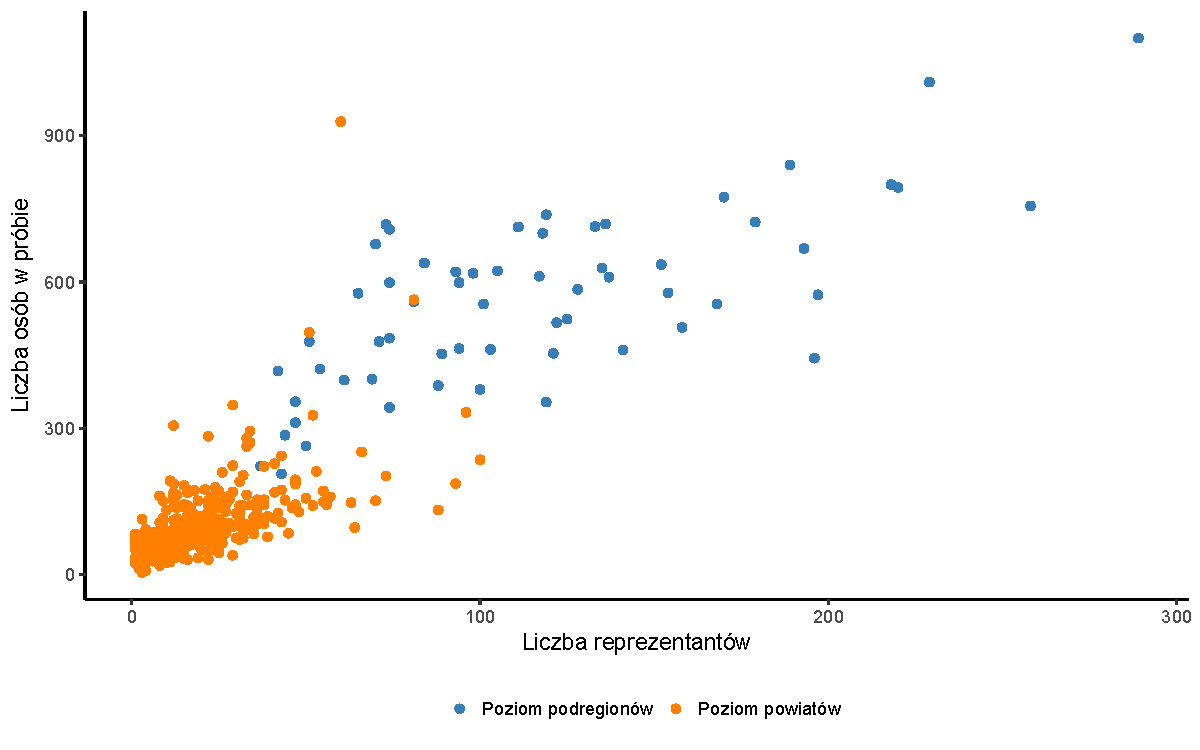
\includegraphics[width=0.8\textwidth]{04_wykresy/liczebnosc_proby_i_reprezentantow-1.pdf}
\caption{Liczba osób w próbie oraz liczba osób ubogich w badaniu EU-SILC 2011 w~przekroju podregionów i powiatów}
\small{Źródło: opracowanie własne na podstawie badania EU-SILC 2011.}
\label{fig:proba_reprez}
\end{figure}

Spośród podregionów najmniej licznie były reprezentowane podregiony ełcki (207 osób w~gospodarstwach domowych), stargardzki (223) oraz suwalski (264). Z kolei największą liczbę reprezentantów odnotowano w podregionach kieleckim (1 100), ostrołęcko-siedleckim (1 010) oraz Warszawie (929).

Rozkład próby w powiatach, których liczba jest prawie 6-krotnie większa niż liczba podregionów był odmienny. Cztery powiaty w ogóle nie były reprezentowane w zrealizowanej próbie --- powiat wieruszowski, proszowicki, moniecki oraz włoszczowski. Minimalna liczba osób w reprezentowanym powiecie wynosiła 4 --- powiat rypiński oraz skierniewicki, z kolei najwięcej osób zbadano w Warszawie (929) oraz innych miastach na prawach powiatu takich jak Łódź (564) czy Kraków (497). Sześć podregionów jest równocześnie miastami na prawach powiatu: Łódź, Warszawa, Kraków, Poznań, Szczecin i Wrocław. Zdarzają się także powiaty, przede wszystkim miasta na prawach powiatu, w których liczba osób w próbie była wyższa niż w niektórych podregionach. Przykładowo, w powiecie kieleckim w próbie znalazło się więcej osób aniżeli w całym podregionie łódzkim składającym się z trzech powiatów.

Najmniej reprezentantów osób ubogich odnotowano w Poznaniu (22), na kolejnym miejscu jest Wrocław (29) oraz Szczecin (34). Z kolei najliczniej osoby ubogie występowały w podregionach kieleckim (289), chełmsko-zamojskim (258) oraz ostrołęcko-siedleckim (229).

Analiza prowadzona na poziomie powiatów pokazuje, że w 12 powiatach nie znalazła się ani jedna osoba uboga, co uniemożliwia estymację bezpośrednią dla tych jednostek. Natomiast w~7~powiatach znalazł się tylko 1 reprezentant zbiorowości osób żyjących w niedostatku. Najwięcej osób ubogich zidentyfikowano w powiecie lubelskim (100), na kolejnym miejscu znalazł się powiat kielecki (96), a za nim powiat tarnowski (93).

Pomiędzy liczbą osób w próbie a liczbą reprezentantów występuje silna dodatnia zależność. Współczynnik korelacji rang Spearmana na poziomie podregionów wynosi 0,64, natomiast na poziomie powiatów 0,68.

W przypadku estymacji wskaźnika określającego głębokość ubóstwa wykorzystywane są te same jednostki, co dla stopy ubóstwa, w związku z czym liczebność reprezentantów będzie taka sama.

\subsection{Jakość oszacowań bezpośrednich wskaźników ubóstwa}

Na podstawie liczby zidentyfikowanych osób ubogich z wykorzystaniem estymatora Horvitza-Thompsona oraz wag przekrojowych z badania EU-SILC oszacowano stopę oraz głębokość ubóstwa na poziomie podregionów i powiatów. W pierwszej kolejności przeanalizowano zmienność otrzymanych oszacowań (por. rys. \ref{fig:zmiennosc_ht}).

\begin{figure}[htp]
\centering
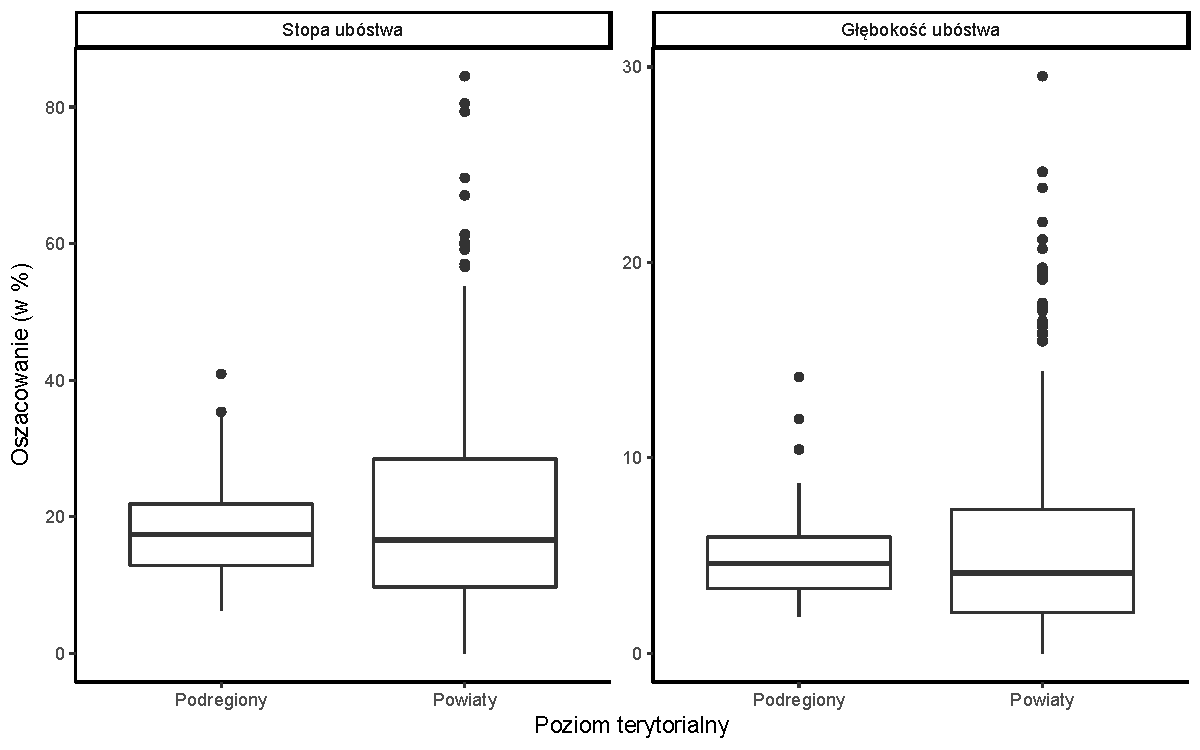
\includegraphics[width=0.8\textwidth]{04_wykresy/zmiennosc_ht-1.pdf}
\caption{Rozkład oszacowań bezpośrednich stopy oraz głębokości ubóstwa w przekroju podregionów i powiatów}
\small{Źródło: opracowanie własne na podstawie badania EU-SILC 2011.}
\label{fig:zmiennosc_ht}
\end{figure}

Wartości przeciętne w ramach każdego z badanych wskaźników w analizowanych przekrojach terytorialnych są zbliżone. Średnia wartość stopy ubóstwa w podregionach wynosi 18\%, natomiast na poziomie powiatów 20\%. Mediana w obu przypadkach jest taka sama --- 17\%. Z kolei średni poziom głębokości ubóstwa wynosi 5\% zarówno na poziomie powiatów i podregionów. Główna różnica w rozkładzie wskaźników wynika ze zróżnicowania. Oszacowania stopy ubóstwa na poziomie podregionów charakteryzują się wartością współczynnika zmienności równą 42\%, a dla głębokości ubóstwa 48\%. Z kolei na poziomie powiatów te wartości są prawie dwukrotnie wyższe --- 74\% dla oszacowań stopy ubóstwa i 89\% dla oszacowań głębokości ubóstwa. Na poziomie powiatów obserwuje się bardzo małe i duże wartości oszacowań wskaźników ubóstwa --- z jednej strony bliskie zeru, a z drugiej przekraczające 80\%. Występowanie takich wartości stopy czy głębokości ubóstwa w rzeczywistości jest wysoce nieprawdopodobne, co wskazuje na niedoskonałość oszacowań bezpośrednich w sytuacji nielicznej próby.

Kryterium oceny jakości estymowanych wskaźników był względny błąd szacunku będący ilorazem błędu standardowego oszacowania i oceny estymatora (ang. \textit{Relative Root Mean Square Error} --- RRMSE). W publikacjach GUS określany jest on jako wskaźnik precyzji. Istnieją dwa podejścia do estymacji błędu oszacowania. Pierwsze z nich zakłada zastosowanie estymatorów odpowiednich dla prostego schematu losowania. Podejście to wynika z przyjęcia założenia, że małe domeny, dla których dokonywana jest analiza nie były uwzględnione na etapie projektowania badania, a zatem nie należy dla nich wykorzystywać informacji na temat schematu losowania. Z kolei drugie podejście wskazuje, że należy te informacje wykorzystać także przy szacowaniu wariancji dla nieplanowanych domen. Niezależnie jednak od rodzaju prowadzonego badania wykorzystanie złożonego schematu losowania powoduje, że otrzymane błędy oszacowań są wyższe \citep{lehtonen2004}. Jest to szczególnie widoczne w przypadku domen, w których próba jest bardzo nieliczna.

W badaniu EU-SILC są dostępne informacje dotyczące jednostek losowania pierwszego stopnia oraz warstw losowania. Wobec tego możliwa jest estymacja wariancji oszacowań wskaźników ubóstwa z wykorzystaniem zaimplementowanego w badaniu złożonego schematu losowania i metody bootstrap. Otrzymane w ten sposób wyniki zestawiono z oszacowaniami uzyskanymi przy założeniu prostego schematu losowania. W metodzie bootstrap losowano 500 podpróbek.

W ramach oceny jakości wyników otrzymanych na podstawie estymacji bezpośredniej w pierwszej kolejności porównano względne błędy oszacowań oraz liczbę reprezentantów --- osób ubogich w przekroju podregionów. Wyniki przedstawiono na rysunku \ref{fig:prec_ht_podreg}.

\begin{figure}[htp]
\centering
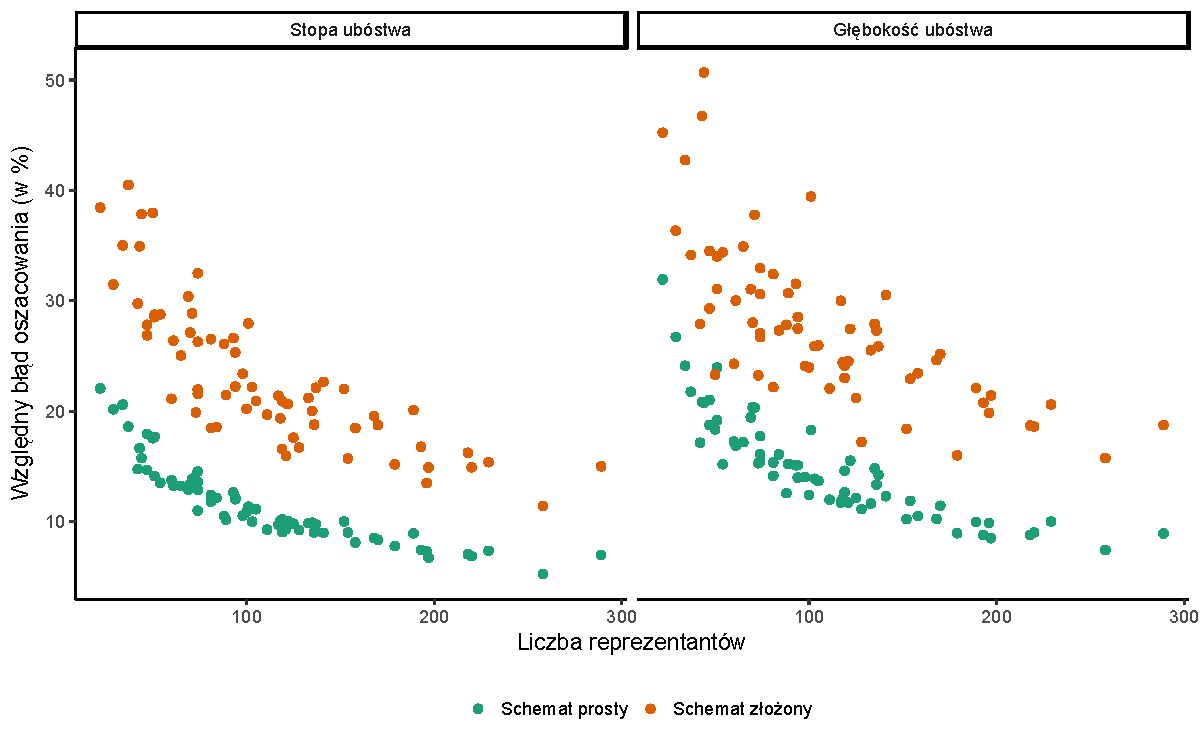
\includegraphics[width=0.8\textwidth]{04_wykresy/precyzja_ht_podreg-1.pdf}
\caption{Porównanie względnych błędów oszacowań i liczby reprezentantów dla stopy oraz głębokości ubóstwa w przekroju podregionów}
\small{Źródło: opracowanie własne na podstawie badania EU-SILC 2011.}
\label{fig:prec_ht_podreg}
\end{figure}

Średnia wartość względnego błędu oszacowania stopy ubóstwa wynosiła 12\% dla schematu prostego i 23\% dla schematu złożonego. W przypadku głębokości ubóstwa przeciętny względny błąd kształtował się na poziomie odpowiednio 15\% i 28\%. Otrzymane wielkości wskazują na to, że wykorzystanie złożonego schematu losowania dwukrotnie zwiększa wartość względnych błędów standardowych w porównaniu do schematu zakładającego losowanie proste. W przypadku stopy ubóstwa dla schematu prostego minimalna wartość wskaźnika precyzji wynosiła 5,2\%, natomiast dla schematu złożonego 11,4\% --- podregion chełmsko-zamojski. Najwyższe względne błędy oszacowań otrzymano dla podregionu m. Poznań (22\%) przy założeniu schematu prostego oraz dla podregionu starogardzkiego (40,5\%) w przypadku schematu złożonego. Wskaźnik głębokości ubóstwa charakteryzuje się wyższymi wartościami względnych błędów oszacowań. Minimum wynoszące 7,4\% dla schematu prostego oraz 15,7\% dla schematu złożonego zanotowano dla podregionu chełmsko-zamojskiego. Najwyższa wartość względnego błędu dla głębokości ubóstwa wynosiła 31,9\% dla podregionu m. Poznań (schemat prosty) oraz 50,7\% dla podregionu szczecińskiego (schemat złożony). Na rysunku można także zaobserwować silną zależność pomiędzy wskaźnikiem precyzji, a liczbą reprezentantów osób ubogich. Współczynnik korelacji rang Spearmana dla wskaźnika stopy ubóstwa wyniósł $r_S=-0,97$ przy założeniu schematu prostego oraz $r_S=-0,86$ przy założeniu schematu złożonego. W przypadku głębokości ubóstwa miary korelacji są następujące: $r_S=-0,92$ dla schematu prostego oraz $r_S=-0,76$ dla schematu złożonego.

Porównano także względne błędy oszacowań na poziomie powiatów. W celu zapewnienia czytelności rysunku \ref{fig:prec_ht_pow} oś OY została ograniczona do wartości 200\%.

\begin{figure}[htp]
\centering
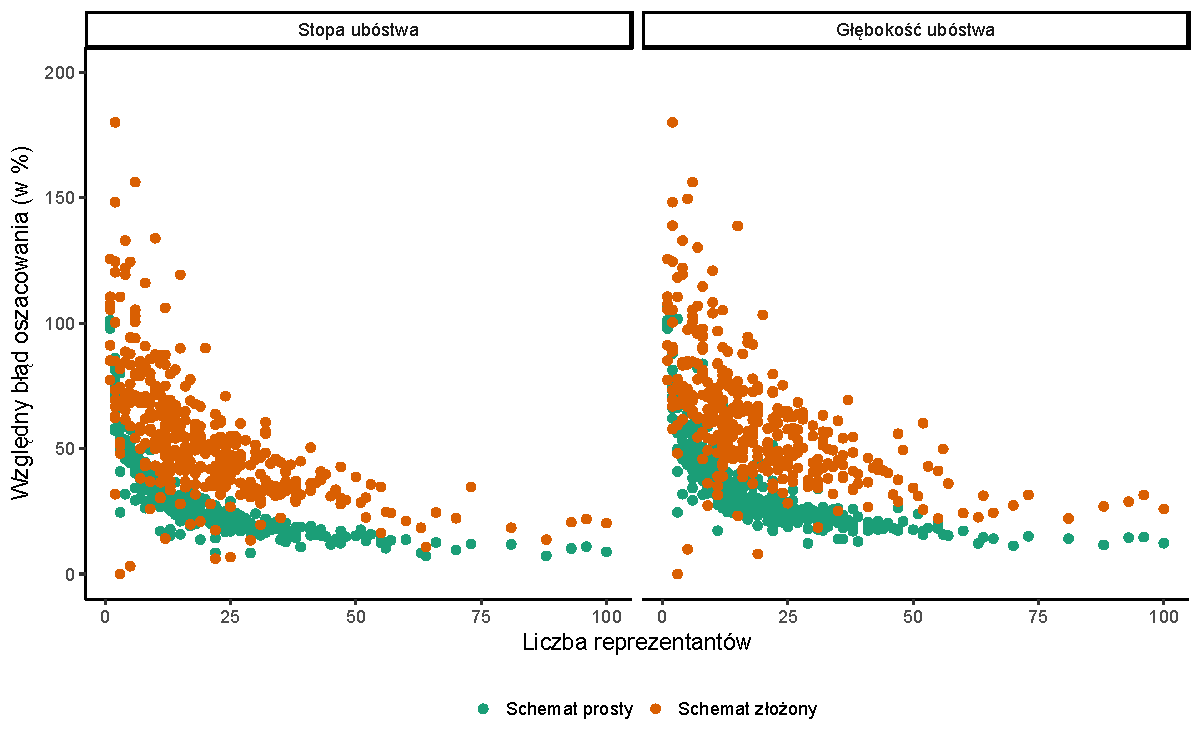
\includegraphics[width=0.8\textwidth]{04_wykresy/precyzja_ht_pow-1.pdf}
\caption{Porównanie względnych błędów oszacowań i liczby reprezentantów dla stopy oraz głębokości ubóstwa w przekroju powiatów}
\small{Źródło: opracowanie własne na podstawie badania EU-SILC 2011.}
\label{fig:prec_ht_pow}
\end{figure}

W przypadku powiatów wykorzystanie złożonego schematu losowania także spowodowało dwukrotny wzrost przeciętnej wartości wskaźnika precyzji. Średni poziom wskaźnika precyzji stopy ubóstwa wyniósł 31\% dla schematu prostego i 59\% dla schematu złożonego. Głębokość ubóstwa cechowały przeciętne wartości błędów równe odpowiednio 36\% i 66\%. O ile maksymalna wartość wskaźnika w przypadku zastosowania prostego schematu losowania wynosiła 107\%, o tyle przy schemacie złożonym było to 749\% (powiat myśliborski w województwie zachodniopomorskim). Ponadto na rysunku nie znalazły się oszacowania błędów wskaźników ubóstwa dla powiatu kolneńskiego (369\%), milickiego (347\%), brzozowskiego (322\%) oraz nidzickiego (246\%). Podobnie jak na poziomie podregionów obserwowana była zależność pomiędzy względnym błędem oszacowania a liczbą reprezentantów. Współczynnik korelacji rang Spearmana wyniósł $r_S=-0,93$ dla stopy ubóstwa w przypadku zastosowania schematu prostego oraz $r_S=-0,72$ w przypadku schematu złożonego. Dla głębokości ubóstwa były to odpowiednio wartości $r_S=-0,90$ i $r_S=-0,70$.

Z teorii metody reprezentacyjnej wiadomo, że estymator bezpośredni jest bardziej efektywny w przypadku zastosowania prostego schematu losowania \citep{bracha1996}. Ponadto wartość błędu oszacowania zależy od liczby jednostek wykorzystanych do estymacji wskaźnika. Ta zależność jest słabsza w przypadku zastosowania złożonego schematu losowania. W związku z tym, w dalszych obliczeniach przyjęto względny błąd wskaźników ubóstwa oszacowany z wykorzystaniem schematu prostego.

\section{Estymacja pośrednia wskaźników ubóstwa}

Kolejnym etapem badania było oszacowanie wskaźników ubóstwa na poziomie podregionów i~powiatów. Z uwagi na wysokie błędy standardowe oszacowań bezpośrednich wskaźników ubóstwa, a tym samym ich niską precyzję, podjęto próbę zastosowania estymacji pośredniej zamiast klasycznego podejścia. Estymacja charakterystyk ubóstwa z wykorzystaniem metod statystyki małych obszarów wymaga użycia tzw. \textit{zmiennych pomocniczych}. Celem zastosowania tych cech jest poprawa jakości estymacji, w związku z czym powinny one pochodzić ze źródeł pozbawionych błędów losowych --- np. z badań pełnych bądź rejestrów administracyjnych. W przypadku stosowania podejścia modelowego kluczowy jest dobór odpowiednich zmiennych, które dobrze opisują zróżnicowanie estymowanych cech. Nieodpowiednia specyfikacja zmiennych niezależnych może powodować obciążenie wyników.

W zależności od wykorzystywanego typu modelu, obszarowego czy jednostkowego, zmienne pomocnicze przyjmują inną postać. W pierwszym przypadku rolę zmiennych niezależnych pełnią zwykle wskaźniki społeczno-demograficzne wyliczone na poziomie danego obszaru --- podregionu bądź powiatu. Głównym źródłem takich cech są ogólnodostępne bazy danych statystycznych np. Bank Danych Lokalnych. Na potrzeby pracy utworzono bazę zmiennych pomocniczych zawierającą 1151 cech ekonomicznych, społecznych oraz demograficznych. Z kolei w podejściu jednostkowym wykorzystuje się informacje dostępne na poziomie pojedynczego gospodarstwa domowego. W tym przypadku konieczny jest dostęp do danych jednostkowych z badania pełnego lub rejestru administracyjnego. Główną przeszkodą w tworzeniu modelu wskaźników ubóstwa jest odróżnienie przyczyn od skutków niedostatku. Przykładowo, osoby ubogie mają zazwyczaj niższe wykształcenie, jednak nie można określić czy niskie wykształcenie zostało spowodowane przez niedostatek czy też bieda panująca w gospodarstwie domowym nie pozwoliła na zdobycie wyższego wykształcenia.

Do obliczeń wykorzystano środowisko R \citep{r2016} w obrębie którego zastosowano funkcje \emph{eblupFH} oraz \emph{eblupSFH} pochodzące z pakietu \emph{sae} \citep{molina-marhuenda2015} w celu oszacowania wskaźników ubóstwa z wykorzystaniem podejścia obszarowego. Do oceny błędu standardowego oraz obciążenia otrzymanych wskaźników zaimplementowano metodę bootstrap z~liczbą replikacji równą 500. Z kolei w aplikacji podejścia jednostkowego korzystano z funkcji \emph{lmer} zaimplementowanej w pakiecie \emph{lme4} \citep{lme42015}, własnych programów oraz funkcji wypracowanych w ramach projektu SAMPLE. Kody wypracowane w programie R zostały zamieszczone w~załączniku.

\subsection{Poziom podregionów}

Rok 2011 był ostatnim rokiem, w którym GUS opublikował dane dotyczące stopy ubóstwa na poziomie województw. Zwiększenie zakresu dostępnych informacji wymaga uwzględnienia niższego poziomu agregacji przestrzennej --- w tym przypadku będzie to poziom podregionów. W latach 2008--2014 w Polsce obowiązywał podział na 66 podregionów. Zmiana nastąpiła w 2015 roku, kiedy to rozdzielono większe podregiony i w ten sposób uzyskano 72 podregionów.

\subsubsection{Modelowanie stopy oraz głębokości ubóstwa na poziomie podregionów}\label{pr:model-podreg}

Punktem wyjścia w pracach nad estymacją wskaźników ubóstwa był model wypracowany w ramach współpracy Głównego Urzędu Statystycznego z Bankiem Światowym \citep{mapowanie2014,wawrowski2014}. Opracowany wówczas model wykorzystywał najprostsze rozwiązania, ponieważ był dedykowany statystyce publicznej. W niniejszej rozprawie zostanie podjęta próba poprawy tego modelu poprzez weryfikację zawartych w nim zmiennych pomocniczych oraz zastosowanie transformacji zmiennej zależnej w celu poprawy własności rozkładu cechy zależnej.

Model będący przedmiotem dyskusji miał na celu estymację wyłącznie stopy ubóstwa i zawierał następujące zmienne niezależne:

\begin{itemize}
\item odsetek osób samotnych powyżej 25 roku życia,
\item liczba pokoi przypadająca na członka gospodarstwa domowego,
\item odsetek gospodarstw domowych posiadających łazienkę,
\item odsetek gospodarstw domowych z dwiema osobami powyżej 25 roku życia z wykształceniem co najwyżej zawodowym,
\item gęstość zaludnienia,
\item stosunek liczby osób wymeldowanych do liczby zameldowanych na pobyt stały w podregionie.
\end{itemize}

W powyższym modelu dwie zmienne niezależne były nieistotne: gęstość zaludnienia oraz stosunek liczby osób wymeldowanych do liczby zameldowanych na pobyt stały w podregionie. Pozostawiono je jednak w modelu ze względów merytorycznych.

W tej części pracy podjęto próbę wypracowania nowego modelu zawierającego wyłącznie istotne zmienne niezależne. Przeanalizowano także możliwości przekształcenia zmiennej zależnej oraz rozszerzono zakres estymacji o wskaźnik głębokości ubóstwa. 

Biorąc pod uwagę dorobek polskich badaczy, jak i publikacje GUS przeanalizowano możliwe determinanty ubóstwa w kontekście ich wykorzystania w modelu ubóstwa. Ze względu na ograniczony dostęp do danych znalezienie ilościowych odpowiedników nie zawsze było możliwe dla wszystkich ustalonych symptomów.

Na podstawie potencjalnych determinant ustalonych w podrozdziale \ref{pr:determinanty} oraz danych dostępnych w Banku Danych Lokalnych dokonano wyboru szeregu wskaźników stanowiących potencjalne zmienne niezależne (pomocnicze) w modelu, w którym zmienną zależną był wskaźnik ubóstwa --- stopa oraz głębokość ubóstwa. Wśród rozpatrywanych zmiennych niezależnych znalazły się m.in. wskaźniki zależności demograficznej, odsetek osób mieszkających na wsi, wskaźniki aktywności ekonomicznej. Analizowano także dane dotyczące rodzin i na ich postawie utworzono wskaźniki określające udział rodzin z dziećmi pozostającymi na utrzymaniu w ogólnej liczbie rodzin w~Polsce z różną liczbą dzieci.

Zmienne opisujące zmienność stopy oraz głębokości ubóstwa zostały wybrane z wykorzystaniem metody krokowej wprzód. W tym celu wykorzystano funkcję \emph{selection} z pakietu FWDselect \citep{fwdselect2015}. Wybrany model był następnie merytorycznie weryfikowany. Badano poprawność znaku stojącego przy parametrze regresji pod kątem wpływu danej zmiennej na poziom ubóstwa oraz statystyczną istotność tego parametru.

W modelu objaśniającym stopę ubóstwa znalazły się następujące zmienne: udział rodzin z~3~dzieci poniżej 24 roku życia pozostających na utrzymaniu w liczbie rodzin z dziećmi poniżej 24 roku życia, odsetek mieszkań posiadających ustęp spłukiwany, udział osób niepełnosprawnych prawnie w liczbie ludności ogółem oraz gęstość zaludnienia. Z kolei w modelu dla głębokości ubóstwa zmienne niezależne były następujące: udział dzieci w wieku do lat 17, na które rodzice otrzymują zasiłek rodzinny w ogólnej liczbie dzieci w tym wieku, udział osób w wieku 20--29 lat pozostających na utrzymaniu w ogólnej liczbie osób w wieku 20-29 lat, udział mieszkań, gdzie przypada powyżej 3 osób na izbę w ogólnej liczbie mieszkań, przeciętna liczba osób w~gospodarstwie domowym oraz stopa bezrobocia rejestrowanego osób pozostających bez pracy powyżej 12 miesięcy.

Rozważono dwa przypadki estymacji stopy oraz głębokości ubóstwa. W pierwszym wykorzystano oryginalne wartości zmiennych zależnych, gdzie wariancja wskaźników została oszacowana z wykorzystaniem metody bootstrap, przy założeniu losowania prostego. W drugim przypadku wykorzystano propozycję transformacji zmiennej z wykorzystaniem pierwiastka arcus sinusa \citep{analpovdata52016}. Wówczas wariancja tak przekształconej cechy była w przybliżeniu równa $\frac{1}{\sqrt{4n}}$. Takie przekształcenie miało zapewnić oszacowanie z przedziału $[0,1]$ oraz ustabilizować wariancję. Punkt odniesienia stanowiły oszacowania bezpośrednie otrzymane po zastosowaniu estymatora Horvitza-Thompsona.

Na rysunku \ref{fig:podreg_trans} porównano rozkłady cech przed i po zastosowaniu transformacji.

\begin{figure}[htp]
\centering
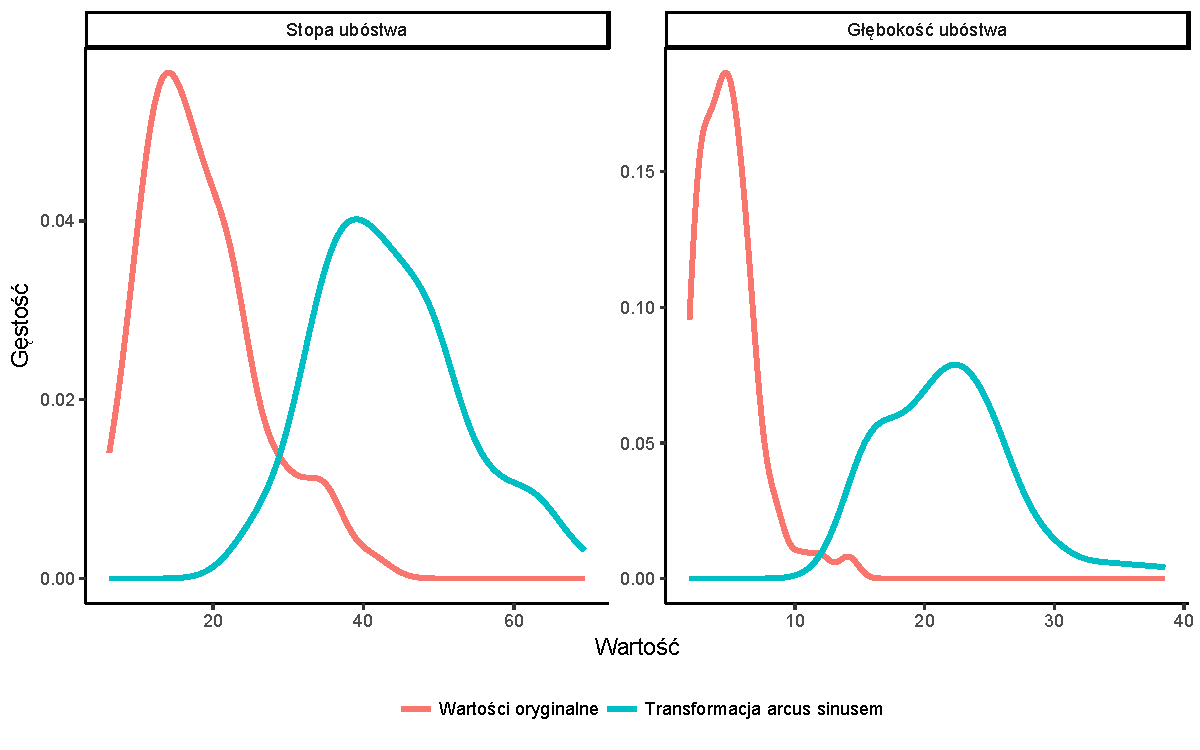
\includegraphics[width=0.8\textwidth]{04_wykresy/podreg_trans-1.pdf}
\caption{Rozkład oszacowań bezpośrednich stopy oraz głębokości ubóstwa na poziomie podregionów --- wartości oryginalne oraz transformowane z wykorzystaniem pierwiastka arcus sinusa}
\small{Źródło: opracowanie własne na podstawie badania EU-SILC 2011.}
\label{fig:podreg_trans}
\end{figure}

Zastosowana transformacja zbliżyła rozkłady obu cech do rozkładu normalnego. Zmianie uległa dyspersja analizowanych wskaźników --- współczynnik zmienności zmalał dwukrotnie, zarówno w przypadku stopy (z 42\% do 22\%), jak i głębokości ubóstwa (z 48\% do 23\%). Trzeci moment centralny oryginalnych wartości stopy ubóstwa wynosił 0,83, natomiast po transformacji wartość ta była równa 0,49. Odpowiednio dla głębokości ubóstwa skośność zmniejszyła się z 1,47 do 0,78. Zastosowana transformacja miała na celu poprawę statystyk dopasowania modelu. W przypadku liniowego modelu dla stopy ubóstwa poprawiono współczynnik $R^2$ z 69,37\% do 72,17\%. Model liniowy dla głębokości ubóstwa charakteryzował się mniejszym przyrostem współczynnika determinacji: z 54,67\% na 54,98\%.

Tak zdefiniowane zmienne zależne oraz wyspecyfikowane cechy niezależne zostały wykorzystane w klasycznym modelu Faya-Herriota oraz modelu Faya-Herriota z przestrzennie skorelowanym efektem losowym.

\subsubsection{Estymacja pośrednia stopy oraz głębokości ubóstwa z wykorzystaniem podejścia obszarowego}

Wybór najlepszego sposobu estymacji stopy oraz głębokości ubóstwa weryfikowany był na podstawie kilku kryteriów: rozkładu względnych błędów oszacowań, kryterium AIC, a także empirycznego obciążenia ocen estymatorów. Błąd średniokwadratowy wszystkich estymatorów został oszacowany z wykorzystaniem metody bootstrap o liczbie replikacji $B=500$, co zapewniło porównywalność wyników.

W celu lepszego zobrazowania przestrzennego aspektu ubóstwa zastosowano model Faya-Herriota z przestrzennie skorelowanym efektem losowym. Podejście to wymagało wyznaczenia macierzy sąsiedztwa dla podregionów w Polsce. W tradycyjnej macierzy sąsiedztwa $W^0$ elementy diagonalne są równe 0, natomiast pozostałe elementy macierzy przyjmują wartość równą 1, w przypadku gdy dwa obszary ze sobą sąsiadują, a 0 w przeciwnym razie. Macierz $W$ konieczną do zastosowania w funkcji \emph{eblupSFH}, otrzymuje się na podstawie $W^0$ poprzez podzielenie każdego elementu w wierszu przez sumę wiersza. W ten sposób uzyskuje się macierz wierszowo-standaryzowaną, której suma każdego wiersza jest równa 1.

Na rysunku \ref{fig:podreg_oszac} przedstawiono rozkład oszacowań wskaźników ubóstwa uzyskanych z~wykorzystaniem estymacji bezpośredniej oraz pośredniej.

\begin{figure}[htp]
\centering
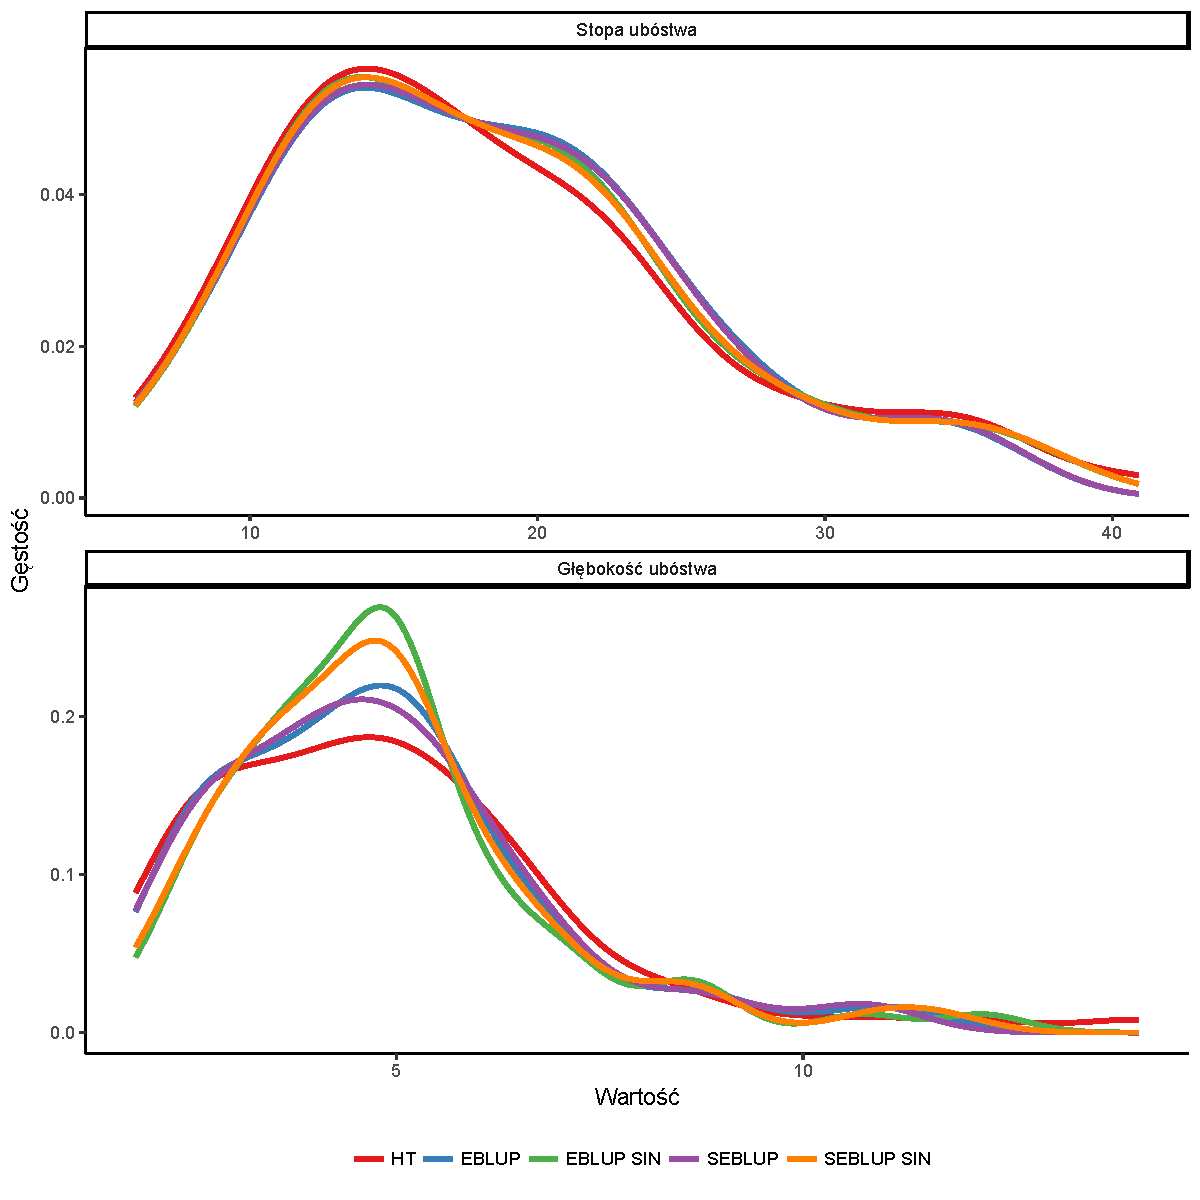
\includegraphics[width=0.8\textwidth]{04_wykresy/model_podreg_oszacowania-1.pdf}
\caption{Rozkład oszacowań bezpośrednich i pośrednich stopy oraz głębokości ubóstwa na poziomie podregionów --- wartości oryginalne oraz transformowane z wykorzystaniem pierwiastka arcus sinusa}
\small{Źródło: opracowanie własne na podstawie badania EU-SILC 2011, NSP 2011 oraz BDL.}
\label{fig:podreg_oszac}
\end{figure}

Rozkłady oszacowań stopy oraz głębokości ubóstwa są do siebie zbliżone. Średnie oszacowania stopy ubóstwa wynoszą 18\% dla wszystkich analizowanych estymatorów oraz 5\% dla głębokości ubóstwa. W przypadku drugiego z badanych wskaźników widoczne są większe rozbieżności w~rozkładach. Mediana oszacowań zarówno w przypadku stopy, jak i głębokości ubóstwa jest nieznacznie niższa od średniej.

Współczynnik korelacji przestrzennej efektów losowych w przypadku stopy ubóstwa wynosił 0,47 oraz 0,53 dla głębokości ubóstwa. Wartości te dotyczą modeli, w których zastosowano transformację zmiennej zależnej. Dla modeli wykorzystujących oryginalne wartości zmiennej $y$~otrzymano odpowiednio 0,46 i 0,41. Kryterium informacyjne Akaikego w przypadku estymacji stopy ubóstwa w modelu Faya-Herriota z przekształceniem zmiennej zależnej wynosiło -193,78, natomiast dla modelu przestrzennego -195,68. Z kolei estymacja głębokości ubóstwa charakteryzowała się mniejszą wartością kryterium AIC: -245,48 dla klasycznego modelu FH w porównaniu do wartości -246,94 dla modelu uwzględniającym korelację przestrzenną. W przypadku modeli szacowanych na podstawie nietransformowanych danych zaobserwowano analogiczną sytuację --- przewaga estymatora SEBLUP nad EBLUP dla stopy ubóstwa oraz niższe kryterium AIC dla estymatora EBLUP w sytuacji, gdy szacowana jest głębokość ubóstwa.

\subsubsection{Ocena precyzji oszacowań}

W celu oceny precyzji szacunków, mając na uwadze z jednej strony zbliżone rozkłady oszacowań wskaźników ubóstwa, zaś z drugiej niejednoznaczne oceny kryterium AIC, porównano rozkłady względnych błędów oszacowań dla poszczególnych estymatorów (por. rys. \ref{fig:podreg_prec}). Zestawienie wartości błędów otrzymanych dla różnych metod estymacji było możliwe dzięki zastosowaniu przy ich wyznaczeniu metody bootstrap.

\begin{figure}[htp]
\centering
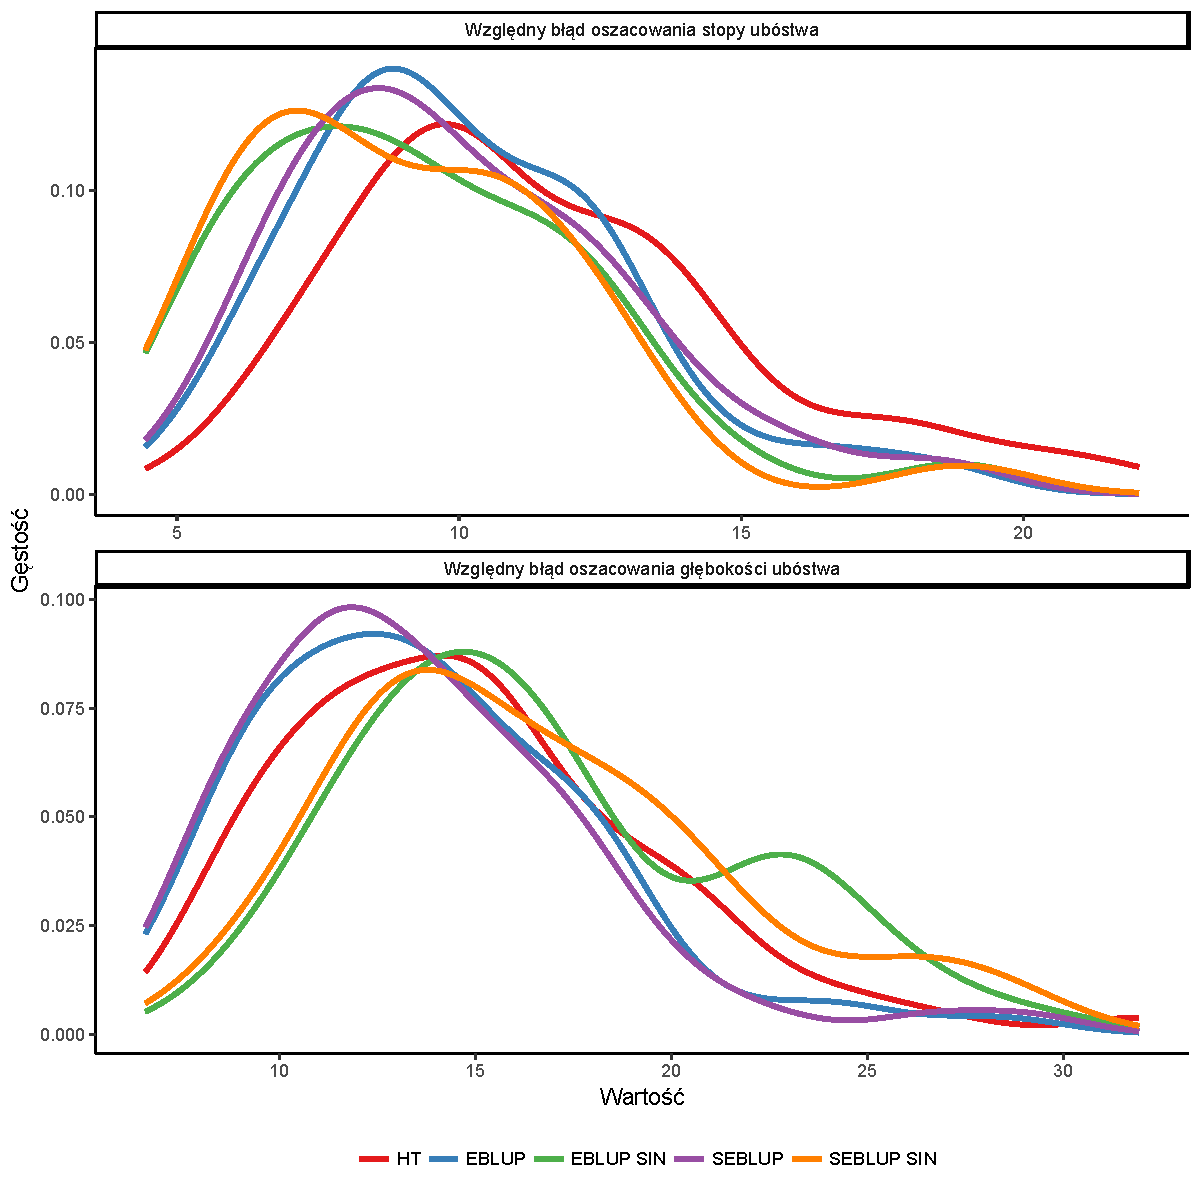
\includegraphics[width=0.8\textwidth]{04_wykresy/model_podreg_precyzja-1.pdf}
\caption{Rozkład względnych błędów oszacowań bezpośrednich i pośrednich stopy oraz głębokości ubóstwa na poziomie podregionów --- wartości oryginalne oraz transformowane z wykorzystaniem pierwiastka arcus sinusa}
\small{Źródło: opracowanie własne na podstawie badania EU-SILC 2011, NSP 2011 oraz BDL.}
\label{fig:podreg_prec}
\end{figure}

W przypadku stopy ubóstwa najniższe średnie oszacowania błędu otrzymano dla estymatora SEBLUP, w którym zastosowano transformację z wykorzystaniem pierwiastka arcus sinusa. Średni poziom tej cechy wynosił 9,11\% w porównaniu do 10,07\% dla estymatora bez transformacji zmiennej zależnej oraz 11,62\% dla oszacowań bezpośrednich. Sytuacja dla wskaźnika głębokości ubóstwa była nieco inna --- poprawę precyzji w odniesieniu do estymacji bezpośredniej obserwuje się w przypadku estymatorów EBLUP i SEBLUP bez transformacji. Natomiast oszacowania pośrednie uzyskane z zastosowaniem przekształcenia pierwiastka arcus sinusa cechują się gorszą precyzją w porównaniu do oszacowań bezpośrednich.

\subsubsection{Ocena obciążenia oszacowań}

W kolejnym kroku ocenie poddano obciążenie rezultatów. Wykorzystano w tym celu test Walda sprawdzający istotność różnic pomiędzy oszacowaniami bezpośrednimi i pośrednimi z uwzględnieniem błędów standardowych ocen szacunków. Wyniki obliczeń przedstawiono w tabeli \ref{tab:wald_podreg}.

\begin{table}[htp]
\caption{Wartości statystyki Walda dla oszacowań pośrednich stopy oraz głębokości ubóstwa na poziomie podregionów}
\label{tab:wald_podreg}
\begin{center}
\begin{tabular}{lrr}
\hline
Estymator & Stopa ubóstwa & Głębokość ubóstwa\tabularnewline
\hline
EBLUP & 12,27 & 9,33\tabularnewline
EBLUP SIN & 5,13 & 21,32\tabularnewline
SEBLUP & 12,76 & 10,75\tabularnewline
SEBLUP SIN & 6,19 & 23,22\tabularnewline
\hline
$\chi^2_{66}$ & \multicolumn{2}{c}{85,96}\tabularnewline
\hline
\end{tabular}\\
\end{center}
\small{Źródło: opracowanie własne na podstawie badania EU-SILC 2011, NSP 2011 oraz BDL.}
\end{table}

We wszystkich przypadkach wartość statystyki empirycznej była mniejsza od wartości statystyki testowej. W związku z tym nie ma podstaw do odrzucenia hipotezy zerowej zakładającej identyczność rozkładów. Zarówno w przypadku oszacowań stopy, jak i głębokości ubóstwa różnice pomiędzy oszacowaniami uzyskanymi z wykorzystaniem estymatora bezpośredniego oraz pośredniego nie różnią się między sobą istotnie statystycznie.

Ocenie poddano także empiryczne obciążenie otrzymanych oszacowań. W tym celu wykorzystano parametryczną metodę bootstrap. Rozkład względnych obciążeń empirycznych przedstawia rysunek \ref{fig:podreg_bias}.

\begin{figure}[htp]
\centering
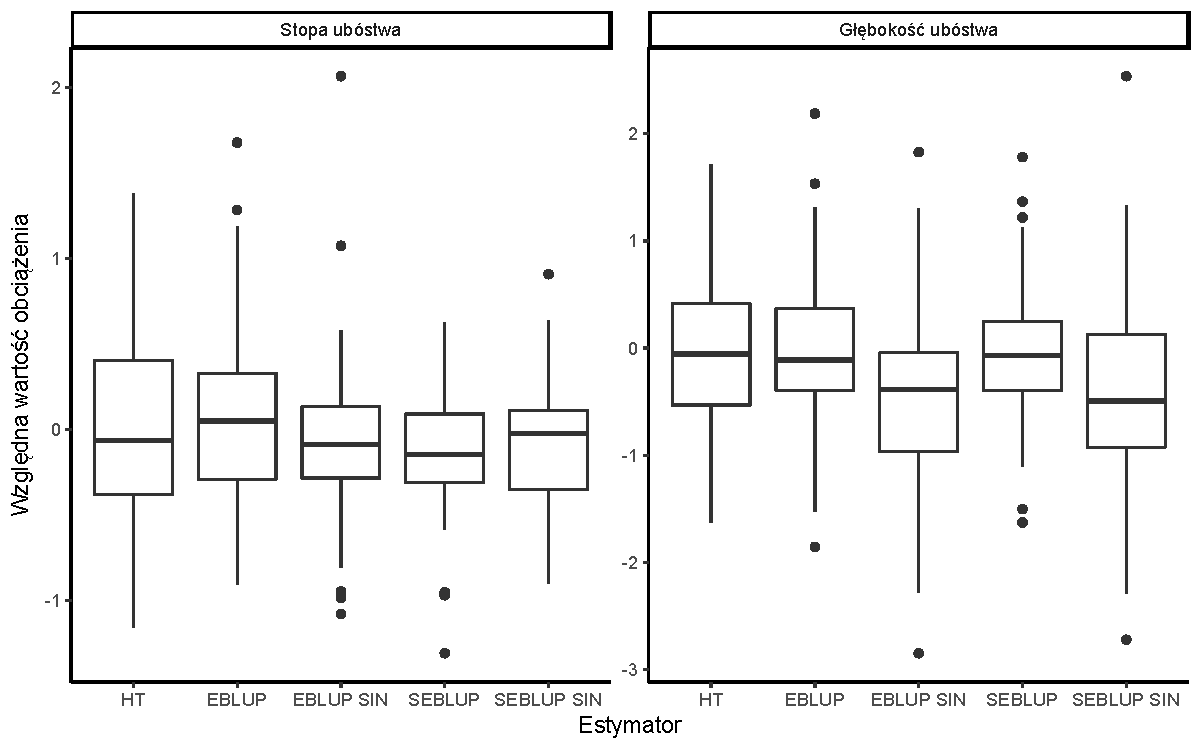
\includegraphics[width=0.8\textwidth]{04_wykresy/fh_podreg_bias-1.pdf}
\caption{Rozkład względnych obciążeń stopy oraz głębokości ubóstwa --- oszacowania bezpośrednie i pośrednie na poziomie podregionów}
\small{Źródło: opracowanie własne na podstawie badania EU-SILC 2011, NSP 2011 oraz BDL.}
\label{fig:podreg_bias}
\end{figure}

Względne empiryczne obciążenie oszacowań stopy ubóstwa dla zastosowanych estymatorów jest niewielkie i dla obu wskaźników nie przekracza 3 punktów procentowych. Miary centralne analizowanej cechy są zbliżone do zera. Jedynie względne obciążenie głębokości ubóstwa estymatorów, w których zastosowano transformacje pierwiastkiem arcus sinusa odbiegają od tego poziomu. Największe niedoszacowanie (2,85 p.p.) obserwowane jest dla estymatora głębokości ubóstwa EBLUP SIN w podregionie suwalskim, a największe przeszacowanie uzyskano w podregionie m.~Poznań (2,54\%) stosując estymator SEBLUP SIN.

Przeprowadzono także test pokrycia, który wykazał, że otrzymane oszacowania znajdują się w 95\% przedziale ufności wyznaczonym przez oszacowania bezpośrednie i pośrednie.

\subsubsection{Ocena własności modelu}

Biorąc pod uwagę wartości oszacowań, względnych błędów ocen estymatorów oraz względnego obciążenia jak optymalny estymator dla obu cech --- stopy oraz głębokości ubóstwa wybrano estymator SEBLUP. Przeprowadzone obliczenia wykazały, że transformacja zmiennej zależnej ma niewielki wpływ na końcowy rezultat, a wręcz może powodować obciążenie rezultatów. Dodatkowo za zastosowaniem oryginalnych wartości zmiennych niezależnych przemawia możliwość łatwej interpretacji współczynników $\beta$ (por. tabela \ref{tab:podreg_beta}).

\begin{table}[htp]
\centering
\caption{Parametry $\beta$ modeli objaśniających stopę oraz głębokość ubóstwa na poziomie podregionów}
\label{tab:podreg_beta}
\begin{tabular}{p{10cm}rrr}
\hline
Zmienna niezależna & $\beta$ & błąd stand. & wartość p \\
\hline
\multicolumn{4}{c}{\textbf{Stopa ubóstwa}}                \\
\hline
Stała   & 0,9033 & 0,2079 & 0,0000 \\
Udział osób niepełnosprawnych prawnie w liczbie ludności ogółem & 1.2933 & 0.3260 & 0.0000\\
Udział rodzin z 3 dzieci poniżej 24 roku życia pozostających na utrzymaniu & 1.1636 & 0,2522 & 0.0000 \\
Gęstość zaludnienia (zmienna binarna) & 0.0390 & 0.0105 & 0.0002 \\
Odsetek mieszkań posiadających ustęp spłukiwany & -0.9871 & 0.2030 & 0.0000 \\
\hline
\multicolumn{4}{c}{\textbf{Głębokość ubóstwa}}            \\
\hline
Stała & -0.0085 & 0.0269 & 0.7520 \\
Udział mieszkań, gdzie przypada powyżej 3 osób na izbę w ogólnej liczbie mieszkań & 0.6498 & 0.2619 & 0.0131 \\
Udział osób w wieku 20--29 lat pozostających na utrzymaniu & 0.2788 & 0.0948 & 0.0033\\
Udział dzieci w wieku do lat 17, na które rodzice otrzymują zasiłek rodzinny & 0.0014 & 0.0005 & 0.0025 \\
Przeciętna liczba osób w gospodarstwie domowym & -0.0250 & 0.0099 & 0.0115 \\
Stopa bezrobocia rejestrowanego osób pozostających bez pracy powyżej 12 miesięcy & -0.2982 & 0.1177 & 0.0113 \\
\hline
\end{tabular}\\
\small{Źródło: opracowanie własne na podstawie badania EU-SILC 2011, NSP 2011 oraz BDL.}
\end{table}

Wśród parametrów $\beta$ oszacowanych dla modelu opisującego stopę ubóstwa, trzy z czterech są dodatnie, co oznacza, że wzrost udziału osób niepełnosprawnych prawnie w liczbie ludności ogółem w podregionie oraz wzrost udziału rodzin z 3 dzieci poniżej 24 roku życia pozostających na utrzymaniu w liczbie rodzin z dziećmi poniżej 24 roku życia w podregionie wpływa także na wzrost stopy ubóstwa. Wyższe wartości stopy ubóstwa będą także obserwowane w podregionach o mniejszej gęstości zaludnienia. Przeciętnie w podregionach o wyższym odsetku mieszkań posiadających ustęp spłukiwany występuje także niższa stopa ubóstwa. Na wielkość głębokości ubóstwa dodatni wpływ mają takie cechy jak udział mieszkań, gdzie przypada powyżej 3 osób na izbę w ogólnej liczbie mieszkań, udział osób w wieku 20 - 29 lat pozostających na utrzymaniu w ogólnej liczbie osób w wieku 20-29 lat oraz udział dzieci w wieku do lat 17, na które rodzice otrzymują zasiłek rodzinny w ogólnej liczbie dzieci w tym wieku. Wzrost przeciętnej liczby osób w gospodarstwie domowym lub stopy bezrobocia rejestrowanego osób pozostających bez pracy powyżej 12 miesięcy wpływa na zmniejszenie wartości głębokości ubóstwa. Wszystkie parametry $\beta$ są istotne, a pomiędzy zmiennymi nie występuje współliniowość o czym świadczą niskie wartości współczynników $VIF$.

Wartości parametru $\hat{\gamma}$ wskazującego jaką część końcowego oszacowania ma stanowić oszacowanie bezpośrednie i regresyjne w przypadku stopy ubóstwa należały do przedziału {[}0,48--0,93{]} z~medianą równą 0,76. Oznacza to, że dla połowy podregionów oszacowanie bezpośrednie stanowiło co najmniej 76\% końcowego oszacowania. Podregionem dla którego przyjęto 93\% oszacowania bezpośredniego było m. st. Warszawa, natomiast dla podregionu gorzowskiego estymator bezpośredni stanowił tylko 48\% końcowego oszacowania. Podregion gorzowski charakteryzował się najwyższa wartością błędu standardowego szacunku bezpośredniego. 

Z kolei przy estymacji głębokości ubóstwa parametr $\hat{\gamma}$ przyjmował wartości z przedziału {[}0,13--0,70{]}, a mediana była na poziomie 0,34. Ta wartość oznacza niską precyzję oszacowań bezpośrednich głębokości ubóstwa, które w większości przypadków miały mniejszy udział w ostatecznym oszacowaniu. Analogicznie jak w przypadku stopy ubóstwa, dla tych samych podregionów otrzymano skrajne wartości parametru $\hat{\gamma}$.

Kolejnym krokiem w analizie było zweryfikowanie założenia modelu dotyczącego normalności reszt oraz efektów losowych. Na rysunku \ref{fig:podreg_model_r} zestawiono wartości reszt standaryzowanych oraz oszacowań uzyskanych z wykorzystaniem estymatora SEBLUP. Ponadto zastosowano test Kołomogorowa-Smirnowa (KS) w celu weryfikacji zgodności rozkładów.

\begin{figure}[htp]
\centering
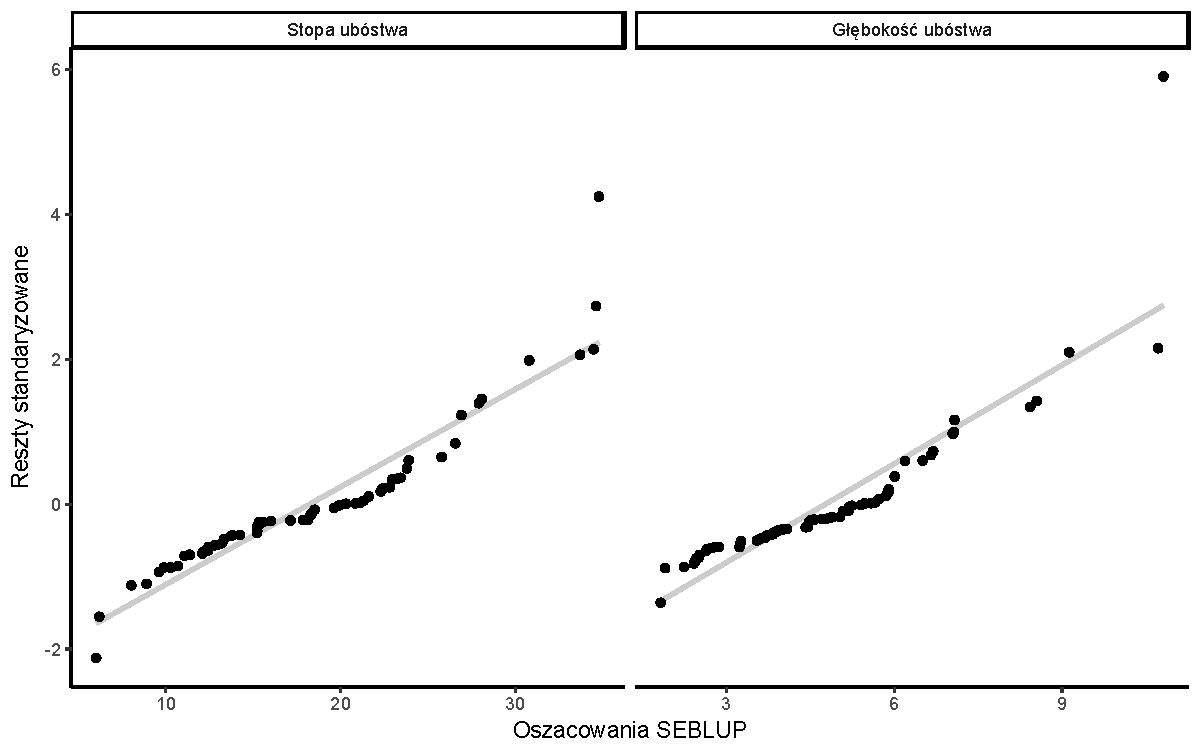
\includegraphics[width=0.8\textwidth]{04_wykresy/fh_podreg_r_model-1.pdf}
\caption{Porównanie reszt standaryzowanych i oszacowań stopy oraz głębokości ubóstwa na poziomie podregionów}
\small{Źródło: opracowanie własne na podstawie badania EU-SILC 2011, NSP 2011 oraz BDL.}
\label{fig:podreg_model_r}
\end{figure}

Na rysunku \ref{fig:podreg_model_r} można zidentyfikować kilka obserwacji odstających --- tzn. takich, dla których wartość reszty standaryzowanej jest większa od 3. W przypadku stopy ubóstwa był to podregion gorzowski oraz tarnowski, natomiast dla głębokości ubóstwa wysokie wartości reszt odnotowano dla podregionu sandomiersko-jędrzejowskiego oraz nowosądeckiego. Oszacowania wskaźników ubóstwa w tych podregionach zaliczyć można do najwyższych. Pomimo tego, w obu przypadkach nie ma podstaw do odrzucenia hipotezy o normalności rozkładu w teście Kołmogorowa-Smirnowa, przyjmując poziom $\alpha=0,05$. Wartość p w teście dla reszt oszacowań stopy ubóstwa była równa 0,2264, natomiast w przypadku głębokości ubóstwa wynosiła 0,0659.

Następnie poddano weryfikacji hipotezę o normalności efektów losowych. Na rysunku \ref{fig:podreg_model_u} przedstawiony jest wykres kwantyl-kwantyl.

\begin{figure}[htp]
\centering
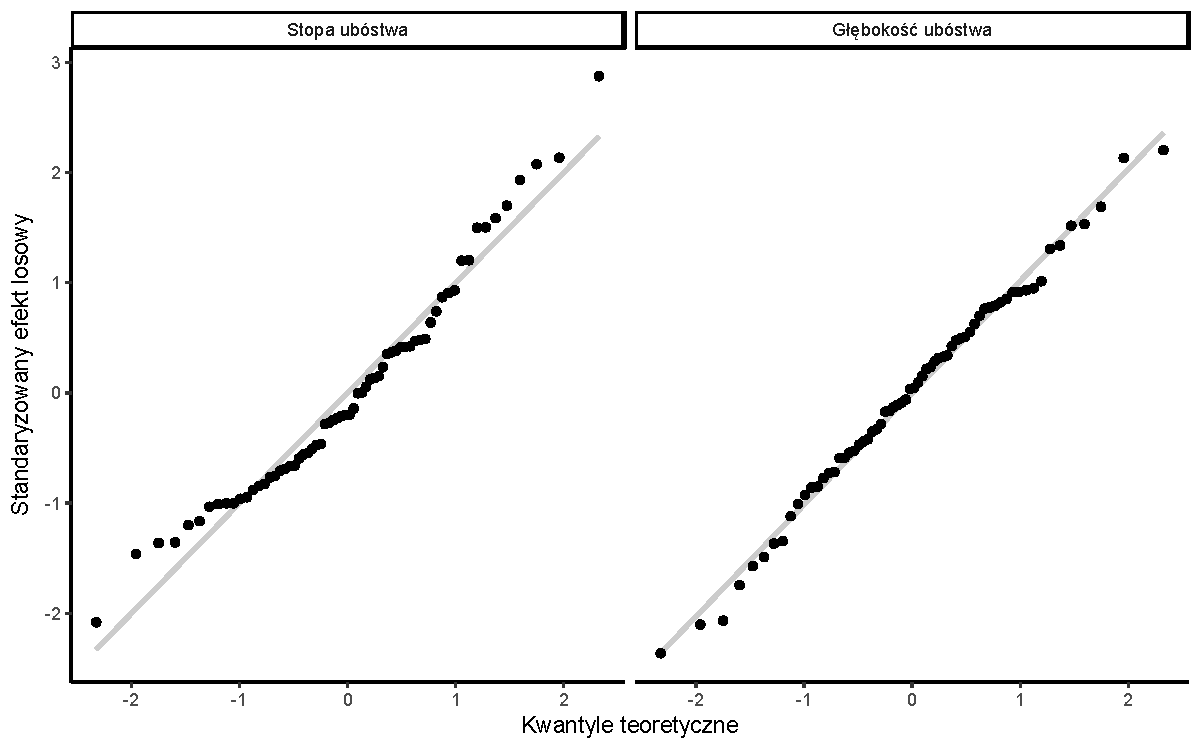
\includegraphics[width=0.8\textwidth]{04_wykresy/fh_podreg_u_model-1.pdf}
\caption{Porównanie kwantyli efektów losowych i kwantyli rozkładu
normalnego stopy oraz głębokości ubóstwa na poziomie podregionów}
\small{Źródło: opracowanie własne na podstawie badania EU-SILC 2011, NSP 2011 oraz BDL.}
\label{fig:podreg_model_u}
\end{figure}

Efekty losowe dla podregionów nieznacznie odbiegają od rozkładu normalnego --- nie zidentyfikowano wartości odstających, a w teście Kołmogorowa-Smirnowa nie ma podstaw do odrzucenia hipotezy zerowej. Wartość p dla obu wskaźników wynosiła 0,9505. Wyżej przeprowadzona weryfikacja modelu wskazuje, że są spełnione założenia, a w związku z tym dobrany model jest poprawny.

Oszacowania otrzymane z wykorzystaniem przestrzennego modelu Faya-Herriota charakteryzują się lepszą precyzją w porównaniu do estymacji bezpośredniej. W tabeli \ref{tab:podreg_prec} zestawiono częstości względnych błędów standardowych oszacowań.

\begin{table}[htp]
\caption{Porównanie precyzji oszacowań bezpośrednich oraz pośrednich stopy oraz głębokości ubóstwa na poziomie podregionów}
\label{tab:podreg_prec}
\centering
\begin{tabular}{lrrrr}
\hline
Wartość RRMSE & $F_0$ HT & $F_0$ SEBLUP & $F_1$ HT & $F_1$ SEBLUP\tabularnewline
\hline
{[}0\%--10\%{]} & 26 & 38 & 9 & 14\tabularnewline
(10\%--20\%{]} & 37 & 28 & 47 & 48\tabularnewline
(20\%--30\%{]} & 3 & 0 & 9 & 4\tabularnewline
(30\%--40\%{]} & 0 & 0 & 1 & 0\tabularnewline
\hline
\end{tabular}\\
\small{Źródło: opracowanie własne na podstawie badania EU-SILC 2011, NSP 2011 oraz BDL.}
\end{table}

Grupując wskaźniki precyzji w przedziały klasowe o rozpiętości 10 punktów procentowych można ocenić skalę poprawy jakości estymacji pośredniej w odniesieniu do estymacji bezpośredniej. W przypadku stopy ubóstwa w przedziale do 10\% znalazło się 58\% podregionów podczas gdy estymacja bezpośrednia umożliwiła taką precyzję tylko dla 26 podregionów. Wartościami w przedziale od 10 do 20 procent cechowało się pozostałe 42\% analizowanych jednostek terytorialnych. W przypadku głębokości ubóstwa zmiany liczebności obserwowane są we wszystkich przedziałach klasowych z wyjątkiem drugiego --- od 10\% do 20\%. W pierwszym przedziale klasowym dla estymatora SEBLUP znalazło się o pięć podregionów więcej w porównaniu do estymatora Horvitza-Thompsona. Jednostek z największym błędem szacunku jest z kolei mniej --- względny błąd oszacowania głębokości ubóstwa dla żadnej jednostki nie przekracza 30\%. Takie rezultaty można uznać za bardzo dobre, zwłaszcza, że GUS za granicę dopuszczającą możliwość publikacji bez tworzenia dodatkowych agregatów przyjmuje wartość RRMSE równą 20\%.

Precyzja oszacowań uzależniona była w dużej mierze od liczby reprezentantów osób ubogich w podregionie. Współczynnik korelacji wskaźnika precyzji i liczby reprezentantów był wysoki i wynosił $r=-0,84$ w przypadku stopy ubóstwa oraz $r=-0,82$ w przypadku głębokości ubóstwa. Stąd też małym błędem oszacowania cechowały się podregiony o dużej liczebności: podregion chełmsko-zamojski, tarnowski oraz puławski. Z kolei najmniej reprezentantów ubogich odnotowano w Poznaniu oraz Wrocławiu, co przełożyło się na wyższy względny błąd oszacowania.

\subsection{Poziom powiatów}

Kolejnym etapem prac nad estymacją stopy oraz głębokości ubóstwa w Polsce była próba oszacowania wskaźników ubóstwa na poziomie powiatów. Powiat ma tę przewagę nad podregionem, że poza jednostką statystyczną jest również jednostką administracyjną. Dzięki temu rezultaty prowadzonych prac mogą być wykorzystywane przez władze powiatów przy planowaniu chociażby polityki społecznej. W analizowanym 2011 roku w Polsce znajdowało się 379 powiatów, w tym 65 miast na prawach powiatu.

Spośród 379 powiatów Polski, cztery nie były w ogóle reprezentowane w próbie badania EU-SILC: wieruszowski (woj. łódzkie), proszowicki (woj. małopolskie), moniecki (woj. podlaskie), włoszczowski (woj. świętokrzyskie). Ponadto, w kolejnych 12 powiatach nie znalazło się żadne ubogie gospodarstwo, co uniemożliwiało uzyskanie szacunków z wykorzystaniem estymatora Horvitza-Thompsona. W związku z tym w analizie rozpatrywano 363 powiaty, dla których udało się oszacować stopę oraz głębokość ubóstwa.

\subsubsection{Estymacja pośrednia stopy oraz głębokości ubóstwa z wykorzystaniem podejścia obszarowego}

Podobnie jak w przypadku wskaźników ubóstwa na poziomie podregionów, w pierwszej kolejności sprawdzono w jaki sposób transformacja z wykorzystaniem pierwiastka arcus sinusa wpływa na rozkład analizowanych cech (por. rysunek \ref{fig:pow_trans}).

\begin{figure}[htp]
\centering
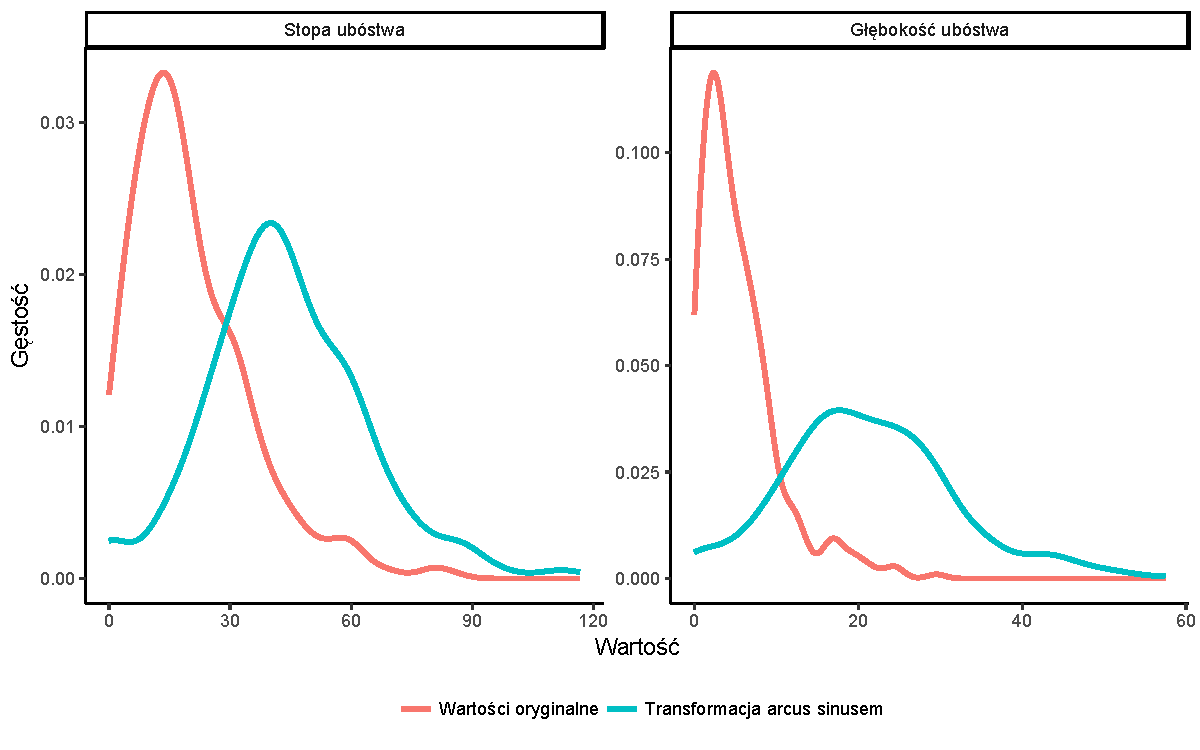
\includegraphics[width=0.8\textwidth]{04_wykresy/pow_trans-1.pdf}
\caption{Rozkład oszacowań bezpośrednich stopy oraz głębokości ubóstwa na poziomie powiatów --- wartości oryginalne oraz transformowane z wykorzystaniem pierwiastka arcus sinusa}
\small{Źródło: opracowanie własne na podstawie badania EU-SILC 2011.}
\label{fig:pow_trans}
\end{figure}

Rozkład bezpośrednich oszacowań stopy oraz głębokości ubóstwa charakteryzował się asymetrią prawostronną --- współczynnik asymetrii wynosi odpowiednio 1,3 i 1,73. Zaobserwowano także bardzo dużą dyspersję wartości wskaźników: 74\% w przypadku stopy ubóstwa oraz 89\% dla głębokości. Wynika to z faktu, że w zbiorze wartości występują oszacowania stopy ubóstwa m.in. na poziomie 84\% spowodowane dominacją reprezentantów osób ubogich w nielicznej próbie. Zastosowanie transformacji umożliwiło zmniejszenie skośności rozkładów --- stopy ubóstwa do wartości współczynnika równej 0,44 oraz głębokości ubóstwa do 0,45. Poprawie uległ także współczynnik zmienności przyjmując wartości odpowiednio 45\% oraz 49\%.

W modelu opracowanym na potrzeby estymacji stopy ubóstwa znalazły się następujące zmienne: udział osób niepełnosprawnych prawnie w liczbie ludności w powiecie, wskaźnik zależności osób w wieku poprodukcyjnym w odniesieniu do liczby osób w wieku produkcyjnym, odsetek osób samotnych powyżej 25 roku życia, udział osób utrzymujących się z~pracy w~rolnictwie w~ogólnej liczbie ludności, wskaźnik zatrudnienia w powiecie, odsetek rodzin z dziećmi do 24 roku życia pozostających na utrzymaniu. Z kolei zmienność głębokości ubóstwa wyjaśniana jest przez udział osób utrzymujących się z pracy w rolnictwie w ogólnej liczbie ludności, odsetek osób samotnych powyżej 25 roku życia, udział osób w wieku 20--29 lat pozostających na utrzymaniu w liczbie osób w wieku 20--29 lat, odsetek gospodarstw zamieszkiwanych przez 4 osoby w liczbie gospodarstw w powiecie, udział osób niepełnosprawnych prawnie w liczbie osób niepełnosprawnych w~powiecie oraz odsetek osób w wieku 20--64 lat posiadających wykształcenie zawodowe (logarytm naturalny).

\begin{figure}[htp]
\centering
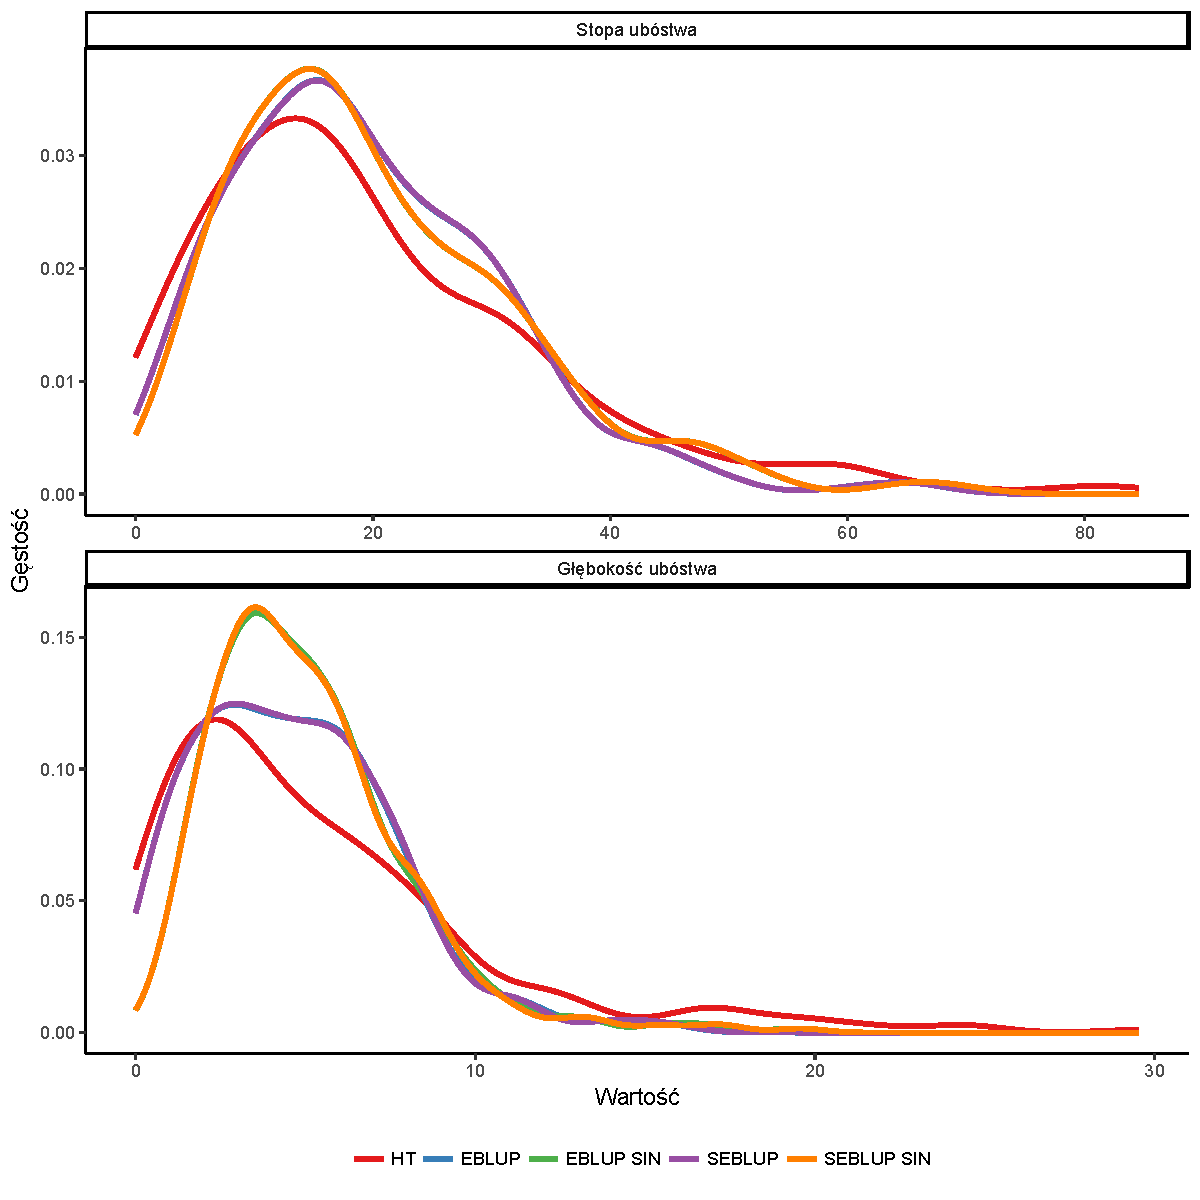
\includegraphics[width=0.8\textwidth]{04_wykresy/fh_powiat-1.pdf}
\caption{Rozkład oszacowań bezpośrednich i pośrednich stopy oraz głębokości ubóstwa na poziomie powiatów --- wartości oryginalne oraz transformowane z wykorzystaniem pierwiastka arcus sinusa}
\small{Źródło: opracowanie własne na podstawie badania EU-SILC 2011, NSP 2011 oraz BDL.}
\label{fig:fh_powiat}
\end{figure}

Oszacowania stopy oraz głębokości ubóstwa uzyskane z wykorzystaniem estymatorów EBLUP i SEBLUP oraz EBLUP i SEBLUP z zastosowaniem transformacji cechują się bardzo zbliżonym rozkładem --- linie opisujące rozkład oszacowań w zasadzie się pokrywają (por. rys. \ref{fig:fh_powiat}). Mediana oszacowań jest równa 17\% dla stopy ubóstwa oraz 4\% dla głębokości. Zastosowanie estymatorów pośrednich powinno przyczynić się do zmniejszenia rozstępu, a tym samym dyspersji estymowanej cechy. Tymczasem maksymalna wartość stopy ubóstwa uzyskana metodami estymacji pośredniej wynosiła 70\%, a głębokości ubóstwa 20\%. Oznacza to, że zmienność oszacowań stopy ubóstwa zmalała z 74\% do 60\%, a oszacowań głębokości ubóstwa z 89\% do 55\%. Z literatury przedmiotu wiadomo, że estymatory obszarowe są przykładem estymatorów ,,kurczących'', co znaczy, że rozstęp oszacowań pośrednich będzie mniejszy od rozstępu oszacowań bezpośrednich \citep{chakraborty2016,rao2015}.

Współczynnik $R^2$ dla modelu liniowego objaśniającego stopę ubóstwa wynosił 25\%, a dla głębokości ubóstwa 20\%. Kryterium informacyjne Akaikego dla estymatora EBLUP w przypadku estymacji stopy ubóstwa wynosiło -507,55, a dla estymatora SEBLUP -505,81. Po zastosowaniu transformacji zmiennej zależnej, model z przestrzennym efektem losowym nadal charakteryzował się wyższą wartością kryterium AIC w porównaniu do klasycznego modelu Faya-Herriota. Przyczyną takiego stanu rzeczy mogły być niskie współczynniki autokorelacji przestrzennej wynoszące $\rho=-0,03$ dla stopy ubóstwa oraz $\rho=0,10$ dla głębokości ubóstwa.

\subsubsection{Ocena precyzji}

Oceny precyzji szacunków dokonano porównując względne błędy oszacowań dla poszczególnych estymatorów (por. rys. \ref{fig:fh_powiat_prec}). 

\begin{figure}[htp]
\centering
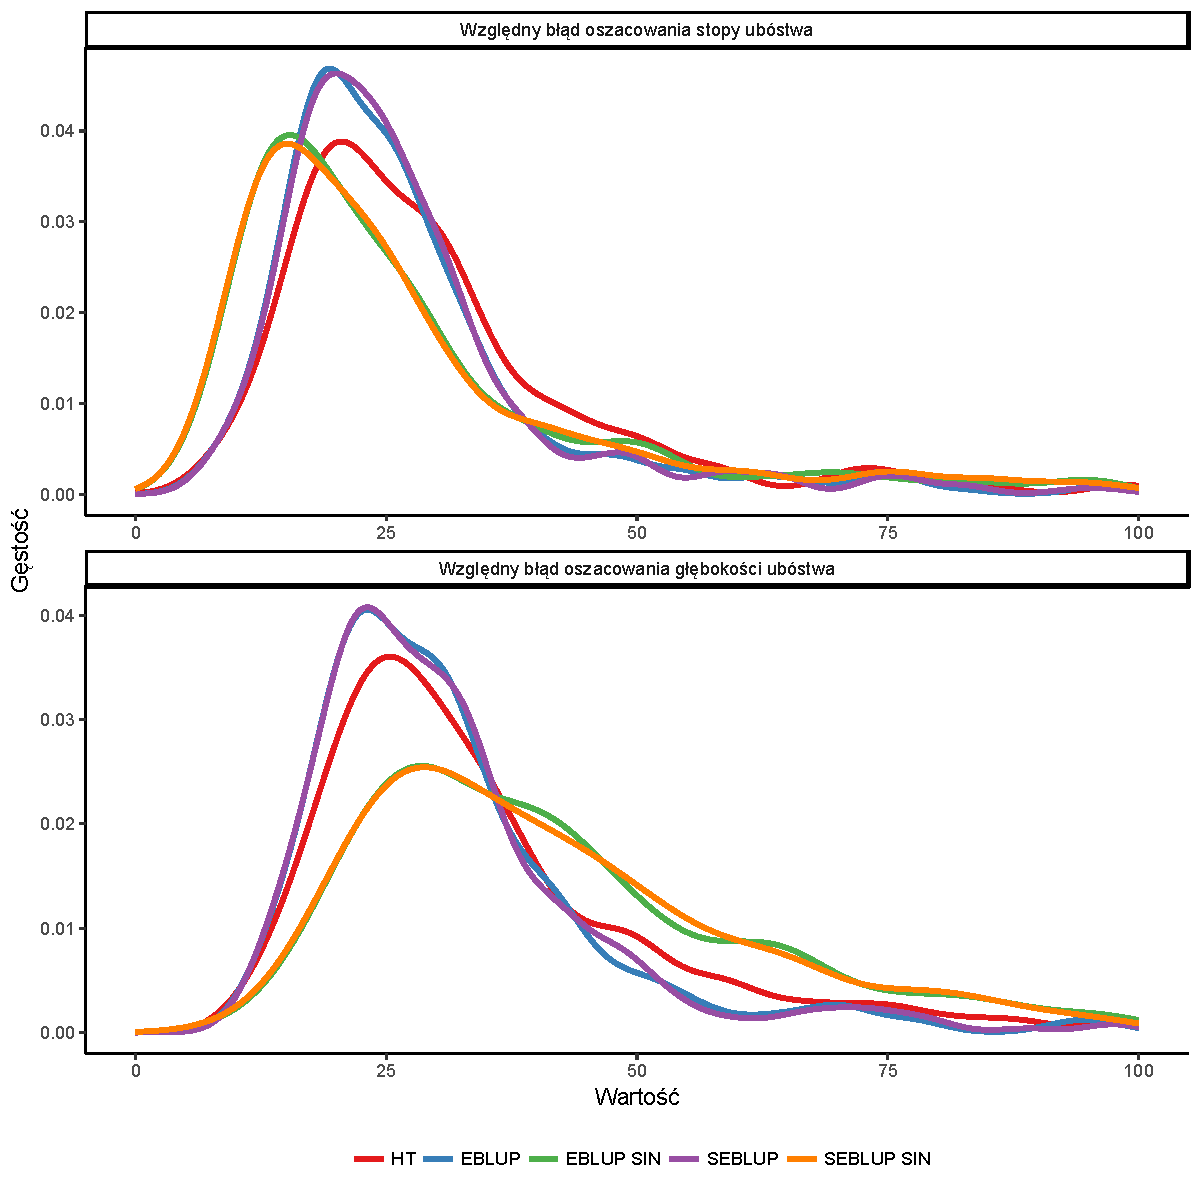
\includegraphics[width=0.8\textwidth]{04_wykresy/fh_pow_prec-1.pdf}
\caption{Rozkład względnych błędów oszacowań bezpośrednich i pośrednich stopy oraz głębokości ubóstwa na poziomie powiatów --- wartości oryginalne oraz transformowane z wykorzystaniem pierwiastka arcus sinusa}
\small{Źródło: opracowanie własne na podstawie badania EU-SILC 2011, NSP 2011 oraz BDL.}
\label{fig:fh_powiat_prec}
\end{figure}

Rozkłady względnych błędów oszacowań wskaźników ubóstwa różnią się w zależności od zastosowanej metody i przekształcenia zmiennej zależnej. W analizowanym przypadku, w którym rozkład wskaźnika precyzji jest asymetryczny, analizę struktury przeprowadzono bazując na miarach pozycyjnych. W przypadku stopy ubóstwa najniższą medianą (22\%) charakteryzowały się oszacowania uzyskane na podstawie transformowanej wartości wskaźnika. Dla estymatorów EBLUP i SEBLUP mediana była wyższa, wynosiła 24\%, ale nadal była to wartość, która wskazywała na większą precyzję podejść pośrednich w porównaniu do estymacji bezpośredniej, gdzie RRMSE wynosił 26\%. Wartości pozostałych miar pozycyjnych charakteryzowały takie same relacje. Z~kolei średnia wartość względnego błędu szacunku dla estymatora bezpośredniego wynosiła 30\%, a~dla estymacji pośredniej była nieco wyższa i wynosiła 33\%--34\%. Świadczy to o tym, że zastosowanie metod pośrednich wpłynęło na nieznaczne pogorszenie przeciętnej precyzji. Należy jednak pamiętać o wadach tej miary tendencji centralnej w przypadku rozkładów asymetrycznych.

\subsubsection{Ocena obciążenia}

Za pomocą testu Walda sprawdzono istotność różnic pomiędzy oszacowaniami pośrednimi oraz bezpośrednimi. Wyniki przedstawiono w tabeli \ref{tab:wald_pow}.

\begin{table}[htp]
\caption{Wartości statystyki Walda dla oszacowań pośrednich stopy oraz głębokości ubóstwa na poziomie powiatów --- podejście obszarowe}
\label{tab:wald_pow}
\centering
\begin{tabular}{lrr}
\hline
Estymator & Stopa ubóstwa & Głębokość ubóstwa\tabularnewline
\hline
EBLUP & 58,83 & 113,13\tabularnewline
EBLUP SIN & 34,74 & 167,96\tabularnewline
SEBLUP & 58,53 & 114,49\tabularnewline
SEBLUP SIN & 34,58 & 168,82\tabularnewline
\hline
$\chi^2_{364}$ & \multicolumn{2}{c}{409,49}\tabularnewline
\hline
\end{tabular}\\
\small{Źródło: opracowanie własne na podstawie badania EU-SILC 2011, NSP 2011 oraz BDL.}
\end{table}

Porównanie statystyk testowych z wartością krytyczną wskazuje, że oszacowania pośrednie są równe co do wartości oczekiwanej, oszacowaniom bezpośrednim. Test pokrycia wykazał, że skonstruowany 95\% przedział ufności nie objął tylko jednej wartości oszacowania stopy ubóstwa i czterech wartości oceny estymatora dla głębokości ubóstwa. 

Następnie ocenie poddano także empiryczne obciążenie otrzymanych oszacowań. Rozkład względnych obciążeń empirycznych przedstawiony jest na rysunku \ref{fig:fh_pow_bias}.

\begin{figure}[htp]
\centering
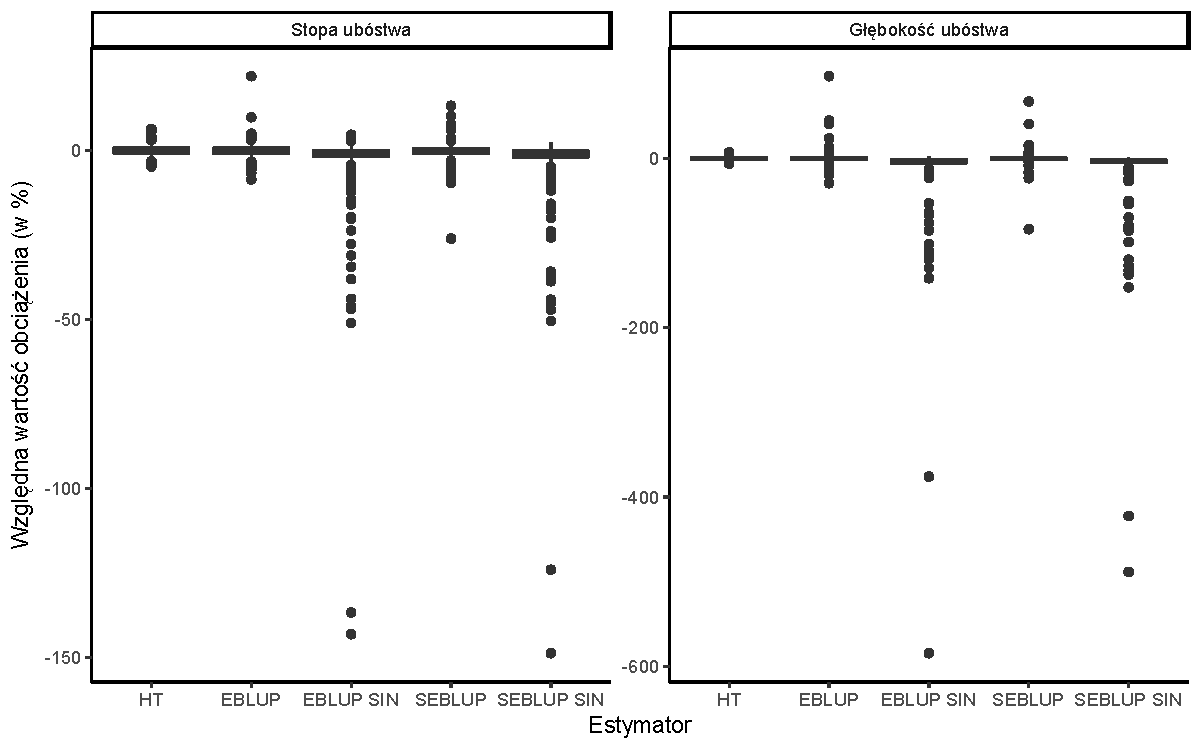
\includegraphics[width=0.8\textwidth]{04_wykresy/fh_pow_bias-1.pdf}
\caption{Rozkład względnych obciążeń stopy oraz głębokości ubóstwa --- oszacowania bezpośrednie i pośrednie na poziomie powiatów}
\small{Źródło: opracowanie własne na podstawie badania EU-SILC 2011, NSP 2011 oraz BDL.}
\label{fig:fh_pow_bias}
\end{figure}

Największe względne obciążenie oszacowań jest obserwowane w przypadku estymatorów, w~których zastosowano transformowaną zmienną zależną. Dla tych estymatorów obserwuje się średnie przeszacowanie na poziomie trzech punktów procentowych w przypadku stopy ubóstwa oraz około dziewięciu punktów procentowych w przypadku głębokości ubóstwa. Z kolei estymatory EBLUP oraz SEBLUP zastosowane na oryginalnych danych charakteryzują się przeciętnym poziomem względnego obciążenia zbliżonym do zera. Zastosowanie transformacji zmiennej doprowadziło do sytuacji, w której udział obciążenia w wartości oszacowania stanowił ponad 100\% oceny estymatora. Najmniejszym rozstępem obciążenia, spośród estymatorów pośrednich, cechował się estymator SEBLUP, w związku z czym został wybrany do dalszej analizy.

Wartości parametru $\hat{\gamma}$ wskazującego jaką część końcowego oszacowania stanowi oszacowanie bezpośrednie i regresyjne w przypadku stopy ubóstwa znajdowały się w przedziale {[}0,15--0,99{]} z~medianą równą 0,85. Oznacza to, że dla połowy powiatów oszacowanie bezpośrednie stanowiło co najmniej 85\% końcowego oszacowania. Z kolei podczas estymacji głębokości ubóstwa parametr $\hat{\gamma}$ przyjmował wartości z przedziału {[}0,01--0,96{]}, a mediana była na poziomie 0,29. Wartości parametru $\hat{\gamma}$ bliskie 1 występują w przypadku powiatów, które charakteryzowały się małym błędem oszacowania --- wówczas estymacja bezpośrednia była uznawana za odpowiednio precyzyjną.

\subsubsection{Ocena własności modelu}

W tabeli \ref{tab:pow_beta} zestawiono parametry $\beta$ wypracowanego modelu.

\begin{table}[htp]
\centering
\caption{Parametry $\beta$ modeli objaśniających stopę oraz głębokość ubóstwa na poziomie powiatów}
\label{tab:pow_beta}
\begin{tabular}{p{10cm}rrr}
\hline
Zmienna niezależna & $\beta$ & błąd stand. & wartość p \\
\hline
\multicolumn{4}{c}{\textbf{Stopa ubóstwa}}                \\
\hline
Stała & -0,7075 & 0,2918 & 0,0153 \\
Odsetek osób samotnych powyżej 25 roku życia & 1,6090 & 0,4108 & 0,0001 \\
Udział osób utrzymujących się z pracy w rolnictwie & 1,3475 & 0,2034 & 0,0000 \\
Odsetek rodzin z dziećmi do 24 roku życia pozostających na utrzymaniu & 1,0213 & 0,3194 & 0,0014 \\
Wskaźnik zależności osób w wieku poprodukcyjnym w odniesieniu do liczby osób w wieku produkcyjnym & 0,6426 & 0,2904 & 0,0269 \\
Udział osób niepełnosprawnych prawnie w liczbie ludności & 0,6389 & 0,2770 & 0,0211 \\
Wskaźnik zatrudnienia & -0,5523 & 0,1697 & 0,0011 \\
\hline
\multicolumn{4}{c}{\textbf{Głębokość ubóstwa}}            \\
\hline
Stała & 0,0150 & 0,0391 & 0,7005 \\
Odsetek osób samotnych powyżej 25 roku życia & 0,2519 & 0,1198 & 0,0354 \\
Udział osób utrzymujących się z pracy w rolnictwie & 0,2366 & 0,0583 & 0,0001 \\
Udział osób w wieku 20--29 lat pozostających na utrzymaniu w liczbie osób w wieku 20--29 lat & 0,1858 & 0,0464 & 0,0001 \\
Udział osób niepełnosprawnych prawnie w liczbie osób niepełnosprawnych & 0,0346 & 0,0233 & 0,1377 \\
Odsetek osób w wieku 20--64 lat posiadających wykształcenie zawodowe (logarytm) & 0,0349 & 0,0098 & 0,0004 \\
Odsetek gospodarstw zamieszkiwanych przez 4 osoby & -0,3176 & 0,1008 & 0,0017 \\
\hline
\end{tabular}\\
\small{Źródło: opracowanie własne na podstawie badania EU-SILC 2011, NSP 2011 oraz BDL.}
\end{table}

W modelu dla stopy ubóstwa na poziomie powiatów jedynie wskaźnik zatrudnienia wpływa na spadek zasięgu ubóstwa w powiecie. Pozostałe zmienne niezależne powodują wzrost wartości wskaźnika ubóstwa. W przypadku modelowania głębokości ubóstwa ujemny znak przy parametrze $\beta$ znajduje się tylko przy zmiennej odsetek gospodarstw zamieszkiwanych przez 4 osoby. Dwie cechy są wspólne dla obu analizowanych wskaźników: odsetek osób samotnych powyżej 25 roku życia oraz udział osób utrzymujących się z pracy w rolnictwie. W obu modelach znalazła się także cecha dotycząca odsetka osób niepełnosprawnych prawnie. Dla stopy ubóstwa jest to udział osób niepełnosprawnych prawnie w liczbie ludności ogółem, a dla głębokości ubóstwa mianownikiem tego wskaźnika jest liczba osób niepełnosprawnych ogółem. Kolejną cechą wspólną modeli jest zmienna przechowująca informację na temat pozostawania na utrzymaniu. Wszystkie zmienne niezależne są istotne oraz nie występuje zjawisko współliniowości, co potwierdzają niskie wartości współczynnika $VIF$.

W kolejnym kroku zweryfikowano założenia modelu dotyczące normalności efektów losowych oraz reszt. Rysunek \ref{fig:fh_pow_r} przedstawia porównanie kwantyl-kwantyl.

\begin{figure}[htp]
\centering
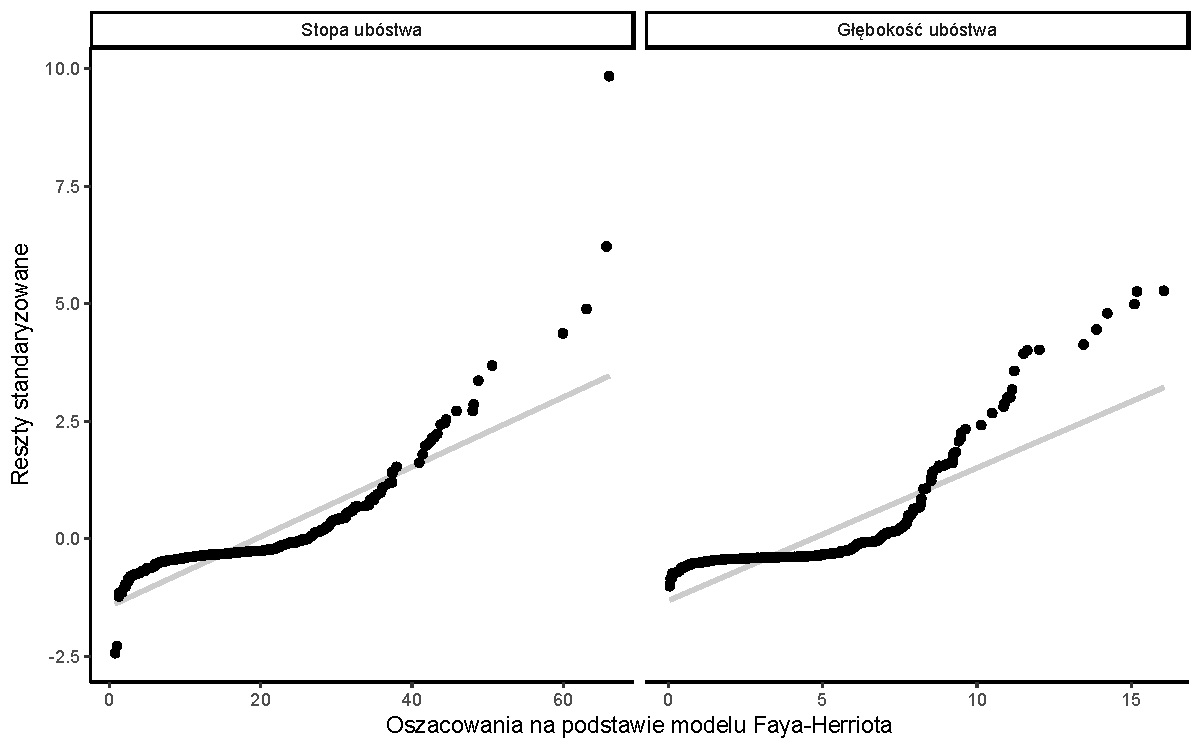
\includegraphics[width=0.8\textwidth]{04_wykresy/fh_pow_r_model-1.pdf}
\caption{Porównanie reszt standaryzowanych i oszacowań stopy oraz głębokości ubóstwa na poziomie powiatów}
\small{Źródło: opracowanie własne na podstawie badania EU-SILC 2011, NSP 2011 oraz BDL.}
\label{fig:fh_pow_r}
\end{figure}

Rozkład reszt dla obu wskaźników wyraźnie odbiega od rozkładu normalnego. Szczególnie duże wartości reszt są związane z wysokimi wartościami oszacowań. Liczba obserwacji w przypadku stopy ubóstwa, dla których reszta standaryzowana przekraczała wartość 3 było 11, natomiast dla głębokości ubóstwa takich powiatów było 12. W teście Kołmogorowa-Smirnowa odrzucono hipotezę zerową o zgodności rozkładów reszt z rozkładem normalnym.

Następnie zweryfikowano hipotezę o normalności efektów losowych porównując standaryzowane wartości z kwantylami rozkładu normalnego (por. rys. \ref{fig:fh_pow_u}).

\begin{figure}[htp]
\centering
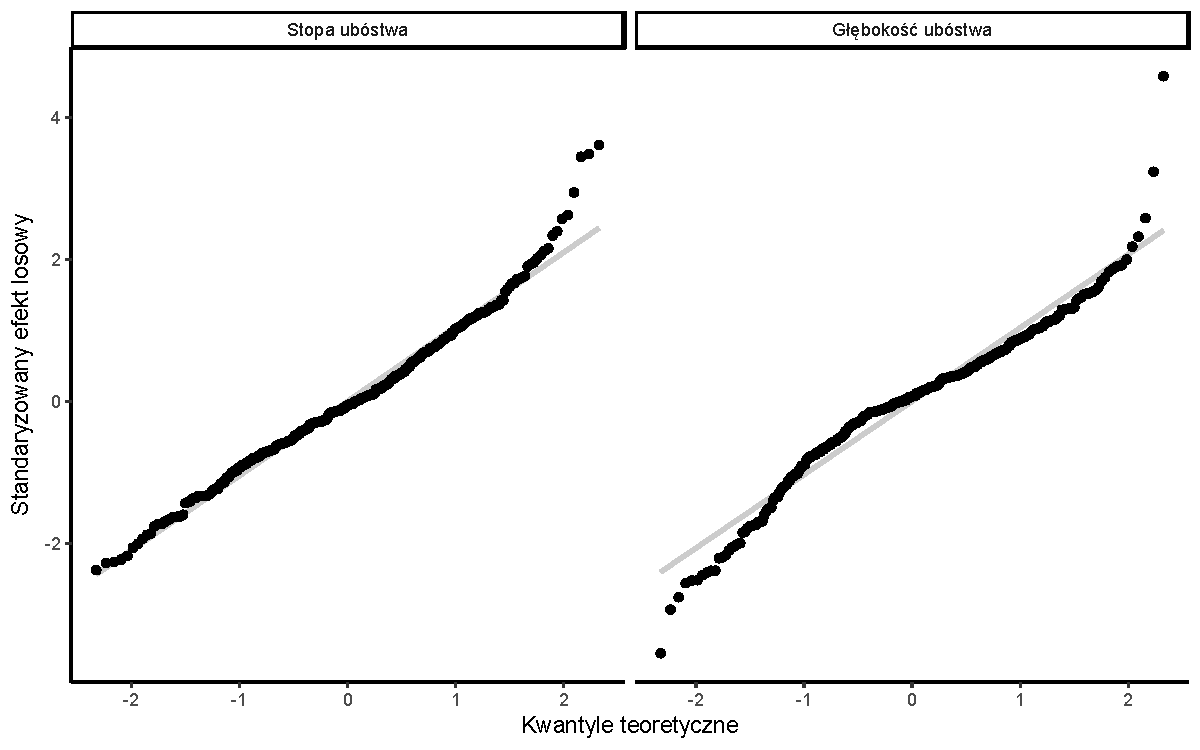
\includegraphics[width=0.8\textwidth]{04_wykresy/fh_pow_u_model-1.pdf}
\caption{Porównanie kwantyli efektów losowych i kwantyli rozkładu normalnego stopy oraz głębokości ubóstwa na poziomie powiatów}
\small{Źródło: opracowanie własne na podstawie badania EU-SILC 2011, NSP 2011 oraz BDL.}
\label{fig:fh_pow_u}
\end{figure}

Efekty losowe na poziomie powiatów dla stopy i głębokości ubóstwa mają rozkład normalny. Największą wartość odstającą odnotowano dla powiatu ełckiego. W obu przypadkach nie ma podstaw do odrzucenia hipotezy zerowej w teście Kołmogorowa-Smirnowa --- wartość p jest równa 0,5798 dla stopy ubóstwa, natomiast dla wskaźnika głębokości ubóstwa $p=0,0835$.

W tabeli \ref{tab:fh_pow_prec} przedstawiono odsetek powiatów należących do przedziału klasowego obejmującego określone wartości względnego błędu oszacowania stopy oraz głębokości ubóstwa uzyskane z wykorzystaniem estymatora bezpośredniego Horvitza-Thomsona oraz pośredniego SEBLUP.

\begin{table}[htp]
\caption{Porównanie precyzji oszacowań bezpośrednich oraz pośrednich stopy oraz głębokości ubóstwa na poziomie powiatów --- podejście obszarowe}
\label{tab:fh_pow_prec}
\centering
\begin{tabular}{lrrrr}
\hline
Wartość RRMSE & $F_0$ HT & $F_0$ SEBLUP & $F_1$ HT & $F_1$ SEBLUP\tabularnewline
\hline
{[}0\%--10\%{]} & 7 & 6 & 0 & 0 \\
(10\%--20\%{]} & 97 & 115 & 46 & 54 \\
(20\%--30\%{]} & 119 & 145 & 129 & 150 \\
(30\%--40\%{]} & 70 & 60 & 93 & 92 \\
powyżej 40\% & 71 & 53 & 96 & 83 \\
\hline
\end{tabular}\\
\small{Źródło: opracowanie własne na podstawie badania EU-SILC 2011, NSP 2011 oraz BDL.}
\end{table}

Niespełnienie wszystkich założeń modelu, występowanie wartości odstających oraz wysokie wartości oszacowań wariancji w podejściu bezpośrednim miały wpływ na fakt, że poprawa precyzji oszacowań pośrednich jest niewielka. Nastąpił wzrost frakcji powiatów znajdujących się w~przedziale od 10 do 20 procent wartości względnego błędu szacunku --- w przypadku stopy ubóstwa z 97 powiatów do 115 jednostek, a dla głębokości ubóstwa o 8 powiatów na korzyść estymacji pośredniej. Największa zmiana liczby powiatów obserwowana jest w przedziale 20\%-30\% wskaźnika precyzji. Pomimo zauważalnych zmian, dla stopy ubóstwa w dalszym ciągu w ponad 100 powiatach obserwuje się wartości względnego błędu oszacowania przekraczającego 30\%. 

\subsubsection{Modelowanie dochodu na poziomie gospodarstwa domowego}

Estymacja z wykorzystaniem modeli na poziomie obszaru w przekroju powiatów nie przyniosła oczekiwanej poprawy jakości oszacowań. Przy takiej liczbie jednostek i dużym zróżnicowaniu zmiennych zależnych estymatory obszarowe nie są w stanie zapewnić odpowiedniego poziomu precyzji. W związku z tym wykorzystano modele na poziomie jednostki.

Modele jednostkowe z kolei bazują na modelowaniu dochodów lub wydatków gospodarstw domowych z wykorzystaniem danych jednostkowych pochodzących z badań pełnych lub zasobów administracyjnych. W tym przypadku dostępność zmiennych niezależnych jest dużo mniejsza od tej występującej dla modeli obszarowych \citep{molina2016}. Dochód gospodarstwa domowego jest objaśniany przez charakterystyki tego gospodarstwa takie jak liczba osób bezrobotnych czy wskaźnik obciążenia demograficznego. Do najważniejszych technik estymacji opartych na modelach jednostkowych należą metody ELL \citep{ell2003}, MQ \citep{mq2006} oraz EB \citep{ebp2010}. Estymacja danego wskaźnika ubóstwa w przypadku tych metod polega na tworzeniu, z wykorzystaniem symulacji Monte Carlo, pseudo-populacji, które stanowią podstawę estymacji wskaźników ubóstwa. Wymienione metody są do siebie bardzo podobne jeśli chodzi o ideę, natomiast można wyróżnić kilka zasadniczych różnic. Metoda ELL nie uwzględnia w ogóle danych pochodzących z badania reprezentacyjnego, w przeciwieństwie do metody EB. Z~kolei metoda MQ jest odporna na obserwacje odstające.

Zastosowanie wyżej przedstawionych metod wymaga opracowania modelu opisującego dochód w gospodarstwach domowych. Jako zmienne pomocnicze wykorzystano cechy demograficzne, ekonomiczne, społeczne oraz terytorialne mierzone na poziomie gospodarstwa. Ponadto, dodano trzy cechy dostępne na poziomie powiatu. W końcowym modelu znalazły się następujące zmienne:

\begin{itemize}
\item poziom gospodarstwa
\begin{itemize}
\item odsetek mężczyzn w gospodarstwie,
\item odsetek osób w wieku 30-44 w gospodarstwie,
\item odsetek osób w wieku 65 lat i więcej w gospodarstwie,
\item odsetek osób bezrobotnych w gospodarstwie,
\item odsetek osób niepełnosprawnych w gospodarstwie,
\item odsetek osób z wykształceniem podstawowym w gospodarstwie,
\item odsetek osób z wykształceniem wyższym w gospodarstwie,
\item wskaźnik obciążenia demograficznego dzieci w gospodarstwie,
\item zmienna binarna - gospodarstwo posiada 1 pokój,
\item zmienna binarna - gospodarstwo posiada 3 pokoje i więcej,
\item zmienna binarna - miejsce zamieszkania: wieś lub miasto do 20 tys. osób,
\end{itemize}
\item poziom powiatu
\begin{itemize}
\item stopa bezrobocia rejestrowanego,
\item odsetek osób zatrudnionych w rolnictwie,
\item wypłacone świadczenie społeczne na 1000 zatrudnionych osób.
\end{itemize}
\end{itemize}

Dla tak określonego zestawu cech oszacowano liniowy model z efektem losowym na poziomie powiatu, w których zmienną zależną był ekwiwalentny dochód gospodarstwa. Model ten będzie określany mianem modelu dwupoziomowego, ze względu na losowy efekt powiatu oraz gospodarstwa domowego.

W tabeli \ref{tab:jedn_beta} przedstawiono parametry $\beta$ oraz oszacowane wariancje efektów losowych.

\begin{table}[htp]
\centering
\caption{Parametry $\beta$ modelu objaśniającego dochód ekwiwalentny na poziomie gospodarstwa domowego}
\label{tab:jedn_beta}
\begin{tabular}{p{10cm}rrr}
\hline
Zmienna niezależna & $\beta$ & błąd stand. & wartość p \\
\hline
wyraz wolny & 24916.24 & 579.64 & 0.0000 \\
odsetek mężczyzn w gospodarstwie & 3233.45 & 474.16 & 0.0000 \\
odsetek osób w wieku 30-44 w gospodarstwie & 1863.55 & 562.68 & 0.0009 \\
odsetek osób w wieku 65 lat i więcej w gospodarstwie & -2959.38 & 382.68 & 0.0000 \\
odsetek osób bezrobotnych w gospodarstwie & -15231.93 & 876.78 & 0.0000 \\
odsetek osób niepełnosprawnych w gospodarstwie & -8649.52 & 745.19 & 0.0000 \\
odsetek osób z wykształceniem podstawowym w gospodarstwie & -2534.25 & 448.32 & 0.0000 \\
odsetek osób z wykształceniem wyższym w gospodarstwie & 19061.33 & 486.28 & 0.0000 \\
wskaźnik obciążenia demograficznego dzieci w gospodarstwie & -3587.74 & 336.20 & 0.0000 \\
gospodarstwo posiada 1 pokój (zmienna binarna) & -2243.68 & 442.58 & 0.0000 \\
gospodarstwo posiada 3 pokoje i więcej (zmienna binarna) & 2824.66 & 272.51 & 0.0000 \\
miejsce zamieszkania: wieś lub miasto do 20 tys. (zmienna binarna) & -2857.61 & 321.58 & 0.0000 \\
\hline
stopa bezrobocia rejestrowanego & -10206.26 & 2632.61 & 0.0001 \\
odsetek osób zatrudnionych w rolnictwie & -8089.02 & 960.84 & 0.0000 \\
wypłacone świadczenie społeczne na 1000 zatrudnionych osób & -1597.30 & 374.01 & 0.0000 \\
\hline
$\sigma_u^2=1388,60$ & & & \\
$\sigma_e^2=13720,70$ & & & \\
\hline
\end{tabular}\\
\small{Źródło: opracowanie własne na podstawie badania EU-SILC 2011, NSP 2011 oraz BDL.}
\end{table}

Wszystkie zmienne niezależne są istotne i mają prawidłowy znak przy parametrze $\beta$. Wyższe wartości czterech zmiennych: odsetek mężczyzn w gospodarstwie, odsetek osób w wieku 30-44 w gospodarstwie, odsetek osób z wykształceniem wyższym w gospodarstwie oraz gospodarstwo posiada 3 pokoje i więcej (zmienna binarna) wpływają także na wzrost dochodu w gospodarstwie. Z kolei parametry przy pozostałych zmiennych mają ujemny znak co oznacza, że wyższe wartości tych cech powodują spadek dochodu w gospodarstwie. Trzy cechy mierzone na poziomie powiatów pokazują wpływ sytuacji ekonomicznej w danym obszarze na dochód pojedynczego gospodarstwa. Wyższa stopa bezrobocia, odsetek osób utrzymujących się z rolnictwa czy wyższy wskaźnik wypłacanych świadczeń z pomocy społecznej negatywnie wpływają na wysokość dochodu gospodarstwa.

%Następnie zweryfikowano normalność reszt oraz efektów losowych w modelu.
%
%\begin{figure}[htp]
%\includegraphics[width=\textwidth]{04_wykresy/doch_norm_lvl1-1.pdf}
%\caption{Porównanie reszt standaryzowanych oraz efektów losowych z kwantylami rozkładu normalnego}
%\small{Źródło: opracowanie własne na podstawie badania EU-SILC 2011, NSP 2011 oraz BDL.}
%\label{fig:doch_norm_lvl1}
%\end{figure}
%
%Wartości na wykresach wskazują, że nie zostały spełnione założenia dotyczące normalności rozkładu. Potwierdza to także przeprowadzony test Kołmogorowa-Smirnowa. Rozkład cechy na poziomie gospodarstwa jest zaburzony przez wcześniej zidentyfikowane wartości odstające - maksymalna wartość reszty standaryzowanej wynosi 37. Obserwacje przekraczające wartość 3 reszt standaryzowanych stanowią tylko 1,17\%. Z kolei na poziomie powiatów odnotowano 3 wartości odstające - m. st. Warszawa, powiat krapkowicki (opolskie) oraz złotoryjski (dolnośląskie). Podobnie na poziomie gmin - wysokie wartości dochodów determinują wielkość efektu losowego na tym poziomie.

W dalszej części pracy wykorzystano model przedstawiony w tabeli \ref{tab:jedn_beta} do estymacji stopy oraz głębokości ubóstwa na poziomie powiatów. W przypadku metody EB zastosowano przekształcenie zmiennej zależnej mające na celu spełnienie założeń o normalności. W metodzie MQ wykorzystano oryginalne wartości ze względu na odporny charakter tego podejścia.

\subsubsection{Estymacja pośrednia stopy oraz głębokości ubóstwa z wykorzystaniem podejścia jednostkowego}

Jak wskazano w podrozdziale \ref{pr:struktura-zmiennych}, rozkład dochodów ekwiwalentnych wyznaczony na podstawie badania EU-SILC charakteryzuje się silną asymetrią prawostronną, co może utrudnić proces modelowania. W celu poprawy własności takiego wektora stosuje się transformacje mające na celu zbliżenie rozkładu cechy do rozkładu normalnego. Do najczęściej stosowanych należy logarytmowanie, logarytmowanie z przesunięciem oraz przekształcenie Boxa-Coxa. W tej części pracy przeanalizowano wszystkie trzy możliwości w celu wyboru transformacji charakteryzującej się najlepszymi własnościami. 

W związku z występowaniem ujemnych wartości dochodu nie jest możliwe bezpośrednie zastosowanie transformacji logarytmicznej. Konieczne jest ustalenie wartości, którą należy dodać do dochodu każdego gospodarstwa, tak aby otrzymany wektor był dodatni. Minimalna wartość dochodu wynosi -7 800 zł, w związku z czym dochód każdego gospodarstwa zostanie powiększony o 7 801 zł, a następnie zlogarytmowany.

Celem transformacji logarytmicznej z przesunięciem jest ustalenie takiej wartości dochodu dodawanej do każdego gospodarstwa, aby rozkład cechy był symetryczny. Wartość tego parametru ustala się w sposób iteracyjny. Zmienna transformowana będzie symetryczna przy wartości przesunięcia równej 7 821,09 zł.

Następnie zastosowano transformację Boxa-Coxa. W tym celu użyto funkcję \emph{BoxCoxTrans} z~pakietu \emph{caret} \citep{caret2016} w programie R. Wykorzystuje ona logarytm wiarygodności do określenia optymalnej wartości parametru $\lambda$. Przeprowadzone obliczenia pozwoliły ustalić wartość parametru na poziomie $\lambda=0,1$.

W tabeli \ref{tab:trans} przedstawiono statystyki opisowe poszczególnych wektorów dochodu w zależności od przyjętego przekształcenia oraz wartości $\lambda$. Ponadto oszacowano model liniowy z wykorzystaniem wcześniej scharakteryzowanych zmiennych niezależnych, w związku z czym w tabeli znajdują się także wartości współczynnika $R^2$.

\begin{table}[htp]
\caption{Statystyki opisowe oraz wartość współczynnika determinacji w zależności od zastosowanej transformacji}
\label{tab:trans}
\centering
\begin{tabular}{lrrrrr}
\hline
Transformacja & $V_s$ & $\alpha_3$ & $\alpha_4$ & $R^2$ & $\lambda$\tabularnewline
\hline
Brak & 71,04 & 6,23 & 117,26 & 25,25 & - \tabularnewline
Logarytm & 4,07 & -0,76 & 30,44 & 30,65 & 7801,00 \tabularnewline
Logarytm z przesunięciem & 4,02 & 0,00 & 9,40 & 31,41 & 7821,09 \tabularnewline
Box-Cox & 6,47 & 0,37 & 6,81 & 31,72 & 0,10 \tabularnewline
\hline
\end{tabular}\\
\small{Źródło: opracowanie własne na podstawie badania EU-SILC 2011.}
\end{table}

Zastosowanie przedstawionych transformacji zmiennych zmniejszyło dyspersję, skośność oraz kurtozę ekwiwalentnego dochodu gospodarstw domowych. Współczynnik zmienności jest najniższy w przypadku transformacji logarytmicznej z przesunięciem. Ponadto rozkład cechy jest w tym przypadku symetryczny. Z kolei kurtoza jest najmniejsza przy przekształceniu Boxa-Coxa. Zastosowanie transformacji zmiennej wpłynęło na wzrost współczynnika determinacji o co najmniej 5 punktów procentowych. Najwyższym współczynnikiem $R^2$ charakteryzuje się model, uwzględniający transformację Boxa-Coxa. W związku z tym takie przekształcenie zastosowano w dalszej analizie.

Wykorzystując dane przedstawione na rysunku \ref{fig:bxcx_norm_lvl1} zweryfikowano normalność reszt oraz efektów losowych w modelu.

\begin{figure}[htp]
\centering
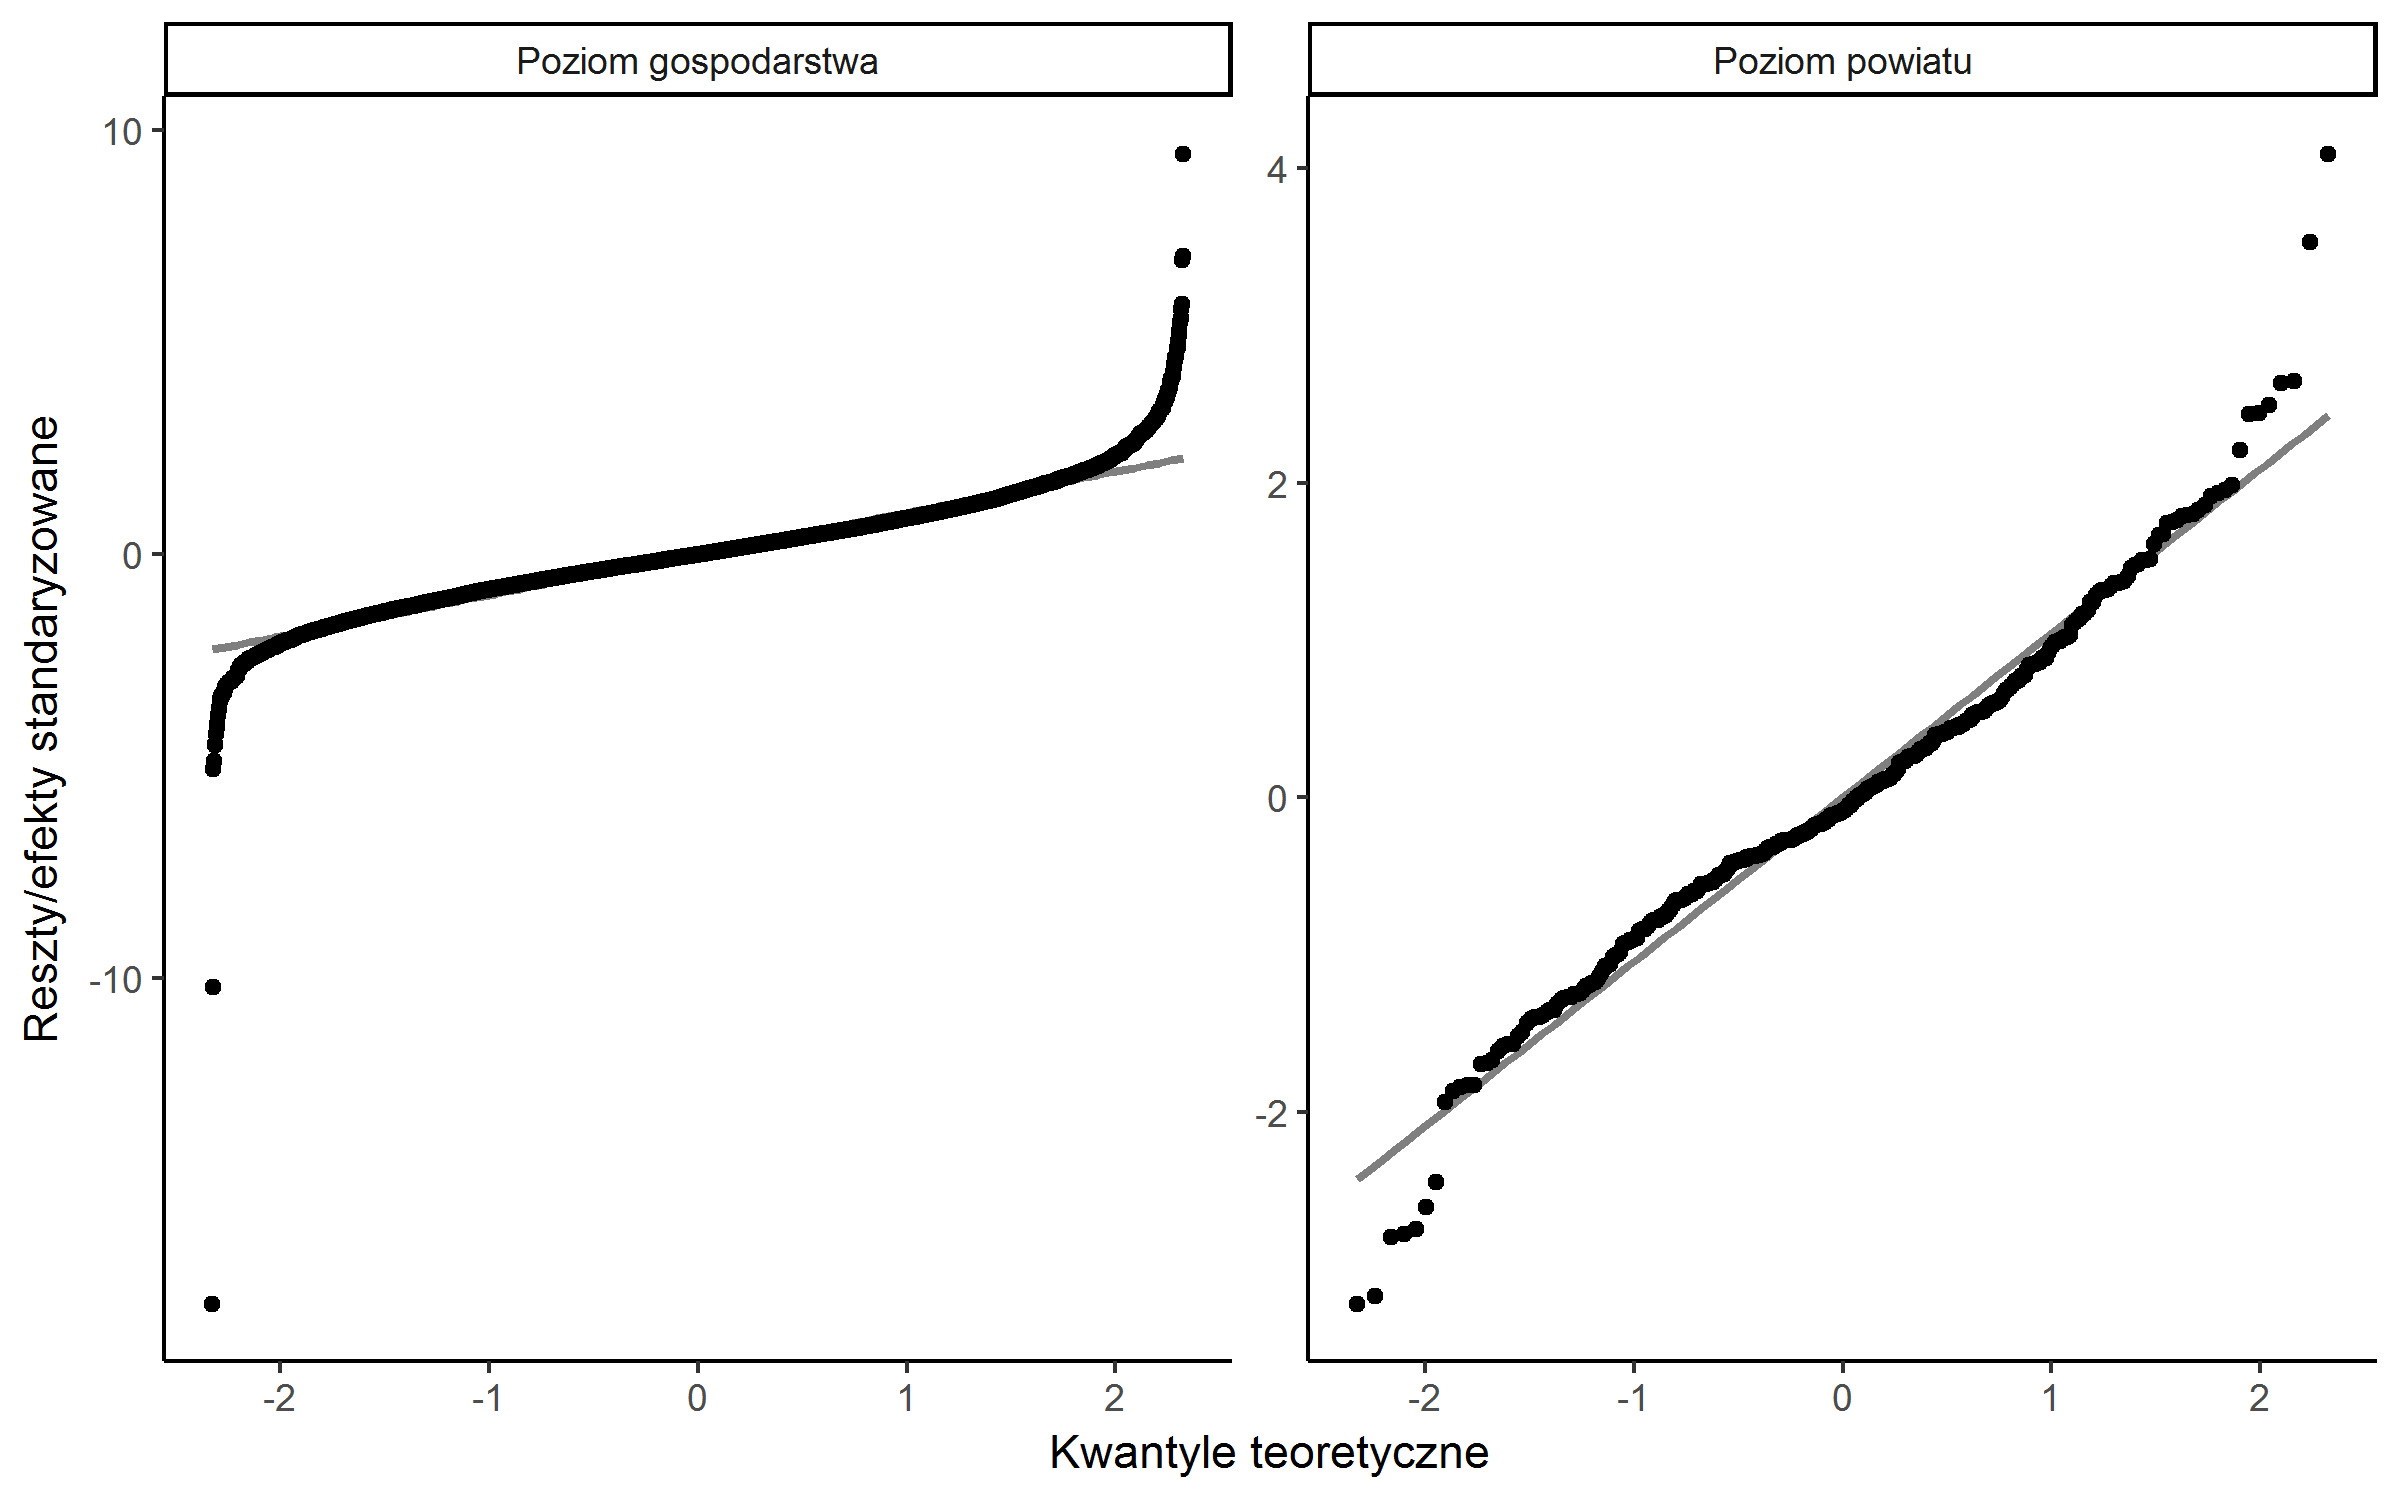
\includegraphics[width=0.8\textwidth]{04_wykresy/bxcx_norm_lvl1-1.png}
\caption{Porównanie reszt standaryzowanych i efektów losowych z kwantylami rozkładu normalnego --- transformacja Boxa-Coxa}
\small{Źródło: opracowanie własne na podstawie badania EU-SILC 2011, NSP 2011 oraz BDL.}
\label{fig:bxcx_norm_lvl1}
\end{figure}

Do najbardziej wpływowych obserwacji na poziomie gospodarstwa należy zaliczyć dwa gospodarstwa o bardzo niskich dochodach, położonych w powiecie świeckim (województwo kujawsko-pomorskie) oraz w m. Katowice. Na poziomie powiatów tylko jedna obserwacja przekracza wartość czterech efektów standaryzowanych --- powiat żuromiński w województwie mazowieckim. Z~wykorzystaniem testu Kołmogorowa-Smirnowa zweryfikowano hipotezę o normalności reszt oraz efektów losowych. Uzyskane reszty na poziomie gospodarstwa nie są zgodne z rozkładem normalnym. Z kolei w przypadku efektów losowych na poziomie powiatu w teście KS nie ma podstaw do odrzucenia hipotezy zerowej - wartość p w modelu dwupoziomowym wynosi 0,8357. Warunkowe kryterium informacyjne AIC \citep{caic2014} dla modelu liniowego z efektem losowym powiatu wynosi 35 257,00 i jest niższe w porównaniu do kryterium AIC policzonego dla zwykłego modelu liniowego: 35 323,13. Stanowi to przesłankę do dalszego stosowania tego typu modelowania.

Na rysunku \ref{fig:eb_mq_lvl1} przedstawiono oszacowania bezpośrednie oraz te uzyskane z zastosowaniem podejścia EB oraz MQ.

\begin{figure}[htp]
\centering
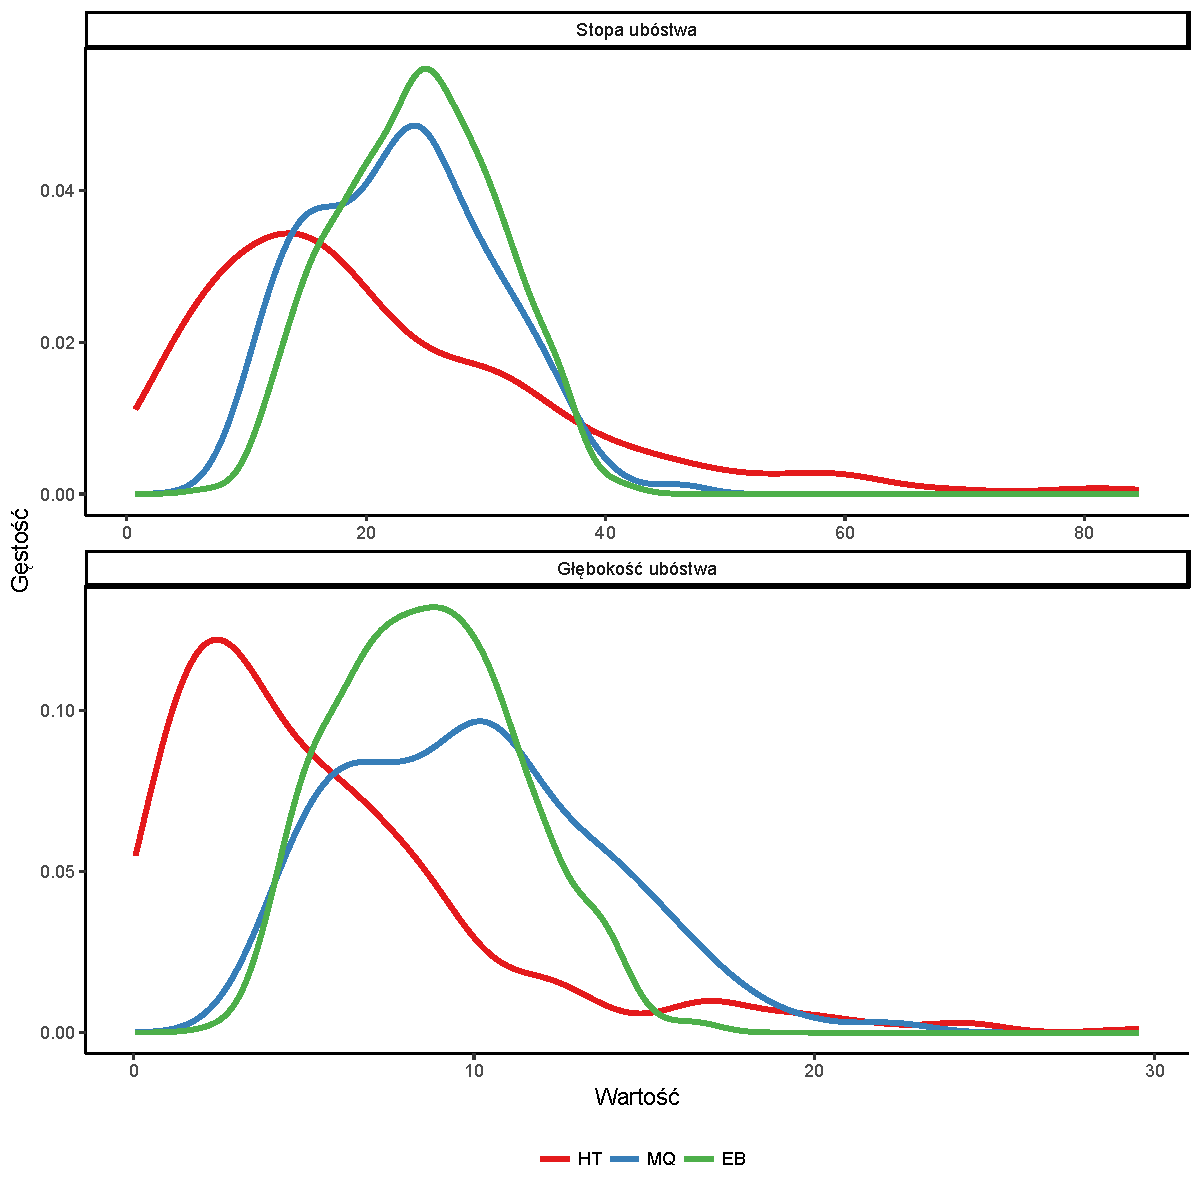
\includegraphics[width=0.8\textwidth]{04_wykresy/eb_mq_lvl1-1.pdf}
\caption{Rozkład oszacowań bezpośrednich oraz pośrednich stopy oraz głębokości ubóstwa na poziomie powiatów}
\small{Źródło: opracowanie własne na podstawie badania EU-SILC 2011, NSP 2011 oraz BDL.}
\label{fig:eb_mq_lvl1}
\end{figure}


Na rysunku można zaobserwować, że oszacowania uzyskane metodami pośrednimi są do siebie podobne, natomiast rozkłady bezpośrednich wskaźników ubóstwa od nich odbiegają. Średnia i mediana oszacowań stopy ubóstwa metodą MQ wynosi 23\%, a w przypadku metody EB 24,4\% i 24,5\% --- wartości te są bardzo zbliżone. Oszacowania bezpośrednie charakteryzują się średnią równą 20,8\% i medianą na poziomie 16,9\%. Ponadto trzeci moment centralny oszacowań EB jest równy 0. Obserwuje się także zmniejszenie rozstępu oszacowań stopy ubóstwa. W podejściu bezpośrednim wartości znajdowały się w przedziale {[}0,7\%--84,5\%{]}, natomiast po zastosowaniu podejścia jednostkowego oszacowania MQ mieszczą się w przedziale {[}6,8\%-46,7\%{]} oraz {[}6,9\%--41,1\%{]} dla metody EB. Podobne obserwacje można poczynić dla wskaźnika głębokości ubóstwa --- mediana oszacowań bezpośrednich wynosi 4,4\%, a dla podejścia MQ 9,9\% oraz 8,6\% dla EB. Rozstęp wskaźnika oszacowanego w sposób bezpośredni wynosi 29,5 punktów procentowych, 20 p.p.~dla oszacowań M-kwantylowych i 14 p.p.~dla oszacowań EB. Estymacja pośrednia wyeliminowała ekstremalnie niskie i wysokie wartości, które w rzeczywistości byłyby raczej nieobserwowane. Zastosowane podejście umożliwiło także estymację dla domen, dla których nie można było zastosować estymatora bezpośredniego.

\subsubsection{Ocena precyzji}

Na rysunku \ref{fig:eb_mq_lvl1_prec} porównano precyzję oszacowań bezpośrednich oraz uzyskanych metodą EB i~MQ.

\begin{figure}[htp]
\centering
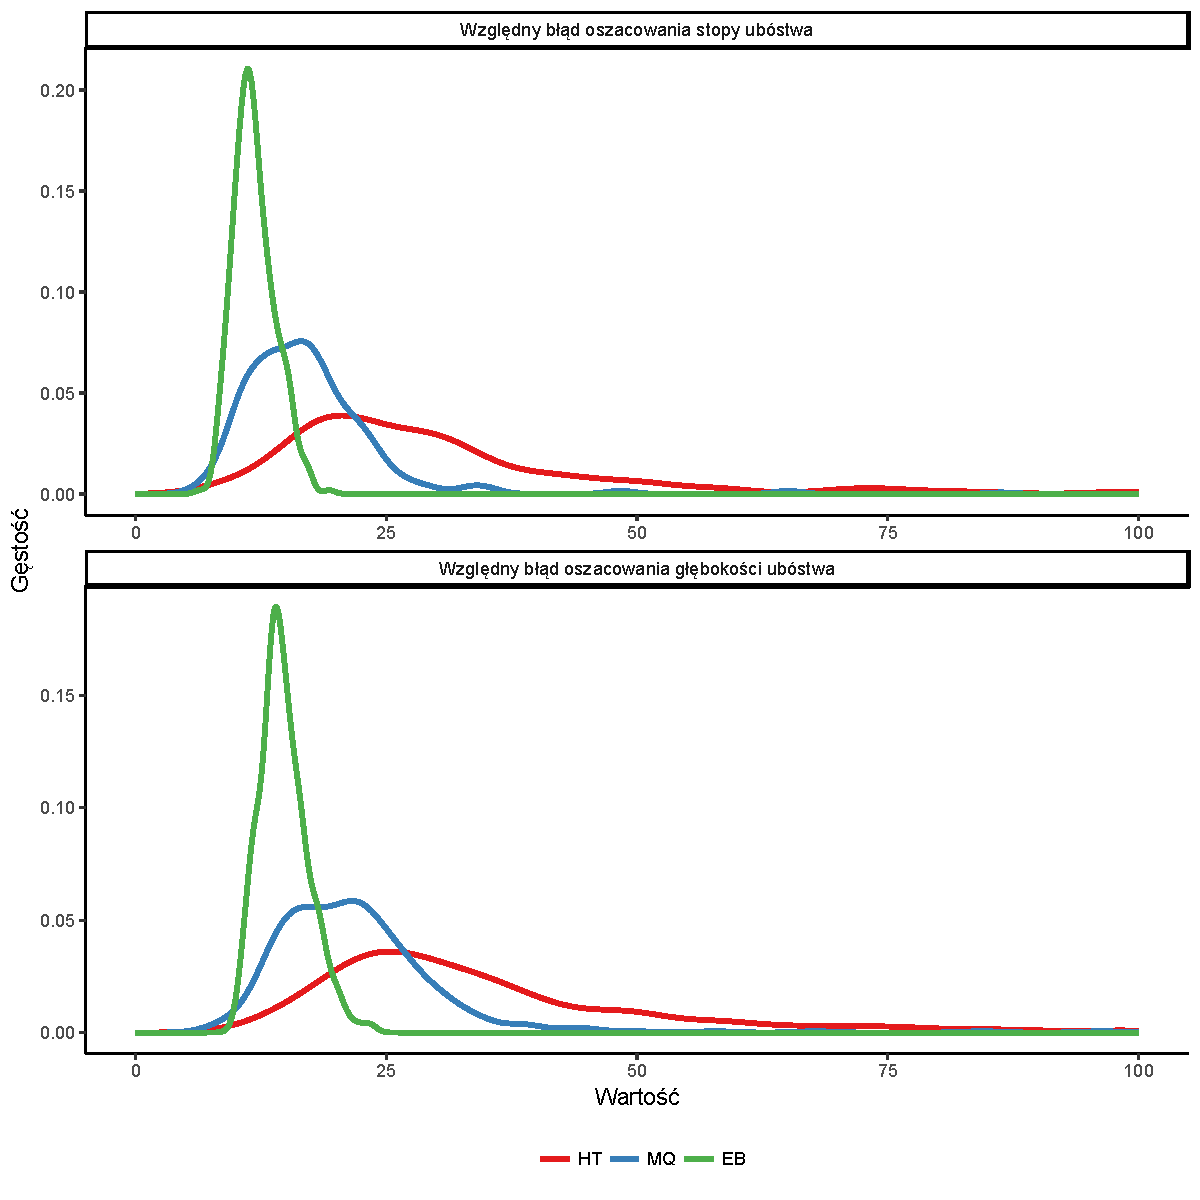
\includegraphics[width=0.8\textwidth]{04_wykresy/eb_mq_lvl1_prec-1.pdf}
\caption{Rozkład względnych błędów oszacowań bezpośrednich oraz pośrednich stopy oraz głębokości ubóstwa na poziomie powiatów}
\small{Źródło: opracowanie własne na podstawie badania EU-SILC 2011, NSP 2011 oraz BDL.}
\label{fig:eb_mq_lvl1_prec}
\end{figure}

Dane przedstawione na rysunku pokazują, że najniższymi wartościami względnych błędów oszacowań charakteryzuje się podejście EB. Rozkład wartości jest leptokurtyczny. Mediana wskaźnika precyzji dla oszacowań bezpośrednich stopy ubóstwa wynosiła 25,9\%, a zastosowanie estymacji pośredniej pozwoliło na obniżenie tej wartości do 16,3\% (MQ) i 11,6\% (EB). Także w~przypadku głębokości ubóstwa zauważalna jest poprawa --- wartość środkowa względnego błędu oszacowań wynosi 14,5\% dla metody EB, 21\% w podejściu MQ oraz 30,3\% stosując estymację bezpośrednią. Największy zysk na precyzji obserwowany jest w przypadku metody EB. 

\subsubsection{Ocena obciążenia}

Z wykorzystaniem testu Walda sprawdzono także istotność różnic pomiędzy oszacowaniami pośrednimi oraz bezpośrednimi. Wyniki przedstawiono w tabeli \ref{tab:wald_pow_eb}.

\begin{table}[htp]
\caption{Wartości statystyki Walda dla oszacowań pośrednich stopy oraz głębokości ubóstwa na poziomie powiatów --- podejście jednostkowe}
\label{tab:wald_pow_eb}
\centering
\begin{tabular}{lrr}
\hline
Estymator & Stopa ubóstwa & Głębokość ubóstwa\tabularnewline
\hline
EB & 2505,89 & 3652,39\tabularnewline
MQ & 1514,17 & 2523,84\tabularnewline
$\chi^2_{364}$ & \multicolumn{2}{c}{409,49} \tabularnewline
\hline
\end{tabular}\\
\small{Źródło: opracowanie własne na podstawie badania EU-SILC 2011, NSP 2011
oraz BDL.}
\end{table}

Oszacowania wskaźników ubóstwa uzyskane z wykorzystaniem metod EB oraz MQ istotnie różnią się od oszacowań bezpośrednich. Taki stan rzeczy wynika z dwóch faktów. Po pierwsze, wykorzystana metoda oceny obciążenia dedykowana jest podejściu obszarowemu. Po drugie, w~estymacji z wykorzystaniem wyżej wymienionych metod jednostkowych nie korzysta się z bezpośrednich oszacowań wskaźników ubóstwa.

Przeprowadzono także test pokrycia dla stopy ubóstwa, w którym 210 oszacowań EB oraz 240 oszacowań MQ znalazło się w 95\% przedziale ufności, co skutkuje odrzuceniem hipotezy zerowej mówiącej o pokryciu rzędu 95\%. W przypadku stopy ubóstwa pokrywające się oszacowania stanowiły 58\% (EB) i 66\% (MQ) wszystkich oszacowań. Dla głębokości ubóstwa pokrycie to jest jeszcze mniejsze i wynosi 45\% dla metody EB i 48\% dla metody MQ.

W tabeli \ref{tab:jedn_prec} przedstawiono precyzję oszacowań w podziale na przedziały klasowe o rozpiętości 10 punktów procentowych.

\begin{table}[htp]
\caption{Porównanie precyzji oszacowań bezpośrednich oraz pośrednich stopy oraz głębokości ubóstwa na poziomie powiatów --- podejście jednostkowe}
\label{tab:jedn_prec}
\centering
\begin{tabular}{lrrrrrr}
\hline
Wartość RRMSE & $F_0$ HT & $F_0$ MQ & $F_0$ EB & $F_1$ HT & $F_1$ MQ & $F_1$ EB \tabularnewline
\hline
{[}0\%--10\%{]} & 0 & 26 & 69 & 0 & 6 & 1 \tabularnewline
(10\%--20\%{]} & 51 & 261 & 310 & 28 & 159 & 367 \tabularnewline
(20\%--30\%{]} & 148 & 75 & 0 & 128 & 168 & 11 \tabularnewline
(30\%--40\%{]} & 94 & 7 & 0 & 104 & 31 & 0 \tabularnewline
powyżej 40\% & 71 & 6 & 0 & 104 & 11 & 0 \tabularnewline
\hline
\end{tabular}\\
\small{Źródło: opracowanie własne na podstawie badania EU-SILC 2011, NSP 2011 oraz BDL.}
\end{table}

Estymacja pośrednia poprawia precyzję oszacowań w porównaniu do estymacji bezpośredniej. Zarówno w przypadku stopy, jak i głębokości ubóstwa największy zysk na precyzji w porównaniu do estymacji bezpośredniej obserwuje się w metodzie EB. Względny błąd oszacowania stopy ubóstwa nie przekracza 20\%. Precyzja oszacowań uzyskanych metodą MQ jest gorsza aniżeli w~podejściu EB, ale i tak zauważalna jest poprawa w odniesieniu do estymacji bezpośredniej.

\section{Podsumowanie}

W niniejszym rozdziale dokonano oceny jakości zmiennych dochodowych pochodzących z badania EU-SILC. Zweryfikowano zgodność dokumentacji badania ze stanem faktycznym, wskazując pojawiające się rozbieżności. Ocenie poddano także skalę stosowania imputacji oraz przeprowadzania wywiadu zastępczego. Stwierdzono, że w przypadku wielu zmiennych dochodowych dotyczących osób informacje pozyskane od respondentów stanowiły mniej niż 50\% wszystkich odpowiedzi --- w pozostałej części korzystano z częściowej lub całkowitej imputacji wartości dochodu. Wywiad zastępczy również przyczyniał się do wzrostu odsetka imputacji. Dużo lepsza była jakość dochodu mierzonego na poziomie gospodarstwa domowego --- w większości przypadków udało się pozyskać kompletną informację. Wyjątek stanowiła kategoria dotycząca dochodu z własności finansowej. Przeprowadzona analiza jakości pozwoliła stwierdzić, że badanie EU-SILC nie jest badaniem doskonałym i należy mieć świadomość czynników mających wpływ na jakość danych wykorzystywanych później do estymacji wskaźników ubóstwa.

% W kwestionariuszu badania EU-SILC jest dział oceniający wywiad indywidualny, gdzie znajduje się pytanie dotyczące korzystania przez respondenta z dokumentów podatkowych podczas odpowiadania na pytania związane z sytuacją dochodową. Niestety ta zmienna nie wchodzi w skład zbiorów wykorzystywanych w analizie. Możliwe, że jej wykorzystanie mogłoby udoskonalić przeprowadzoną analizę.

W drugiej części rozdziału dokonano estymacji stopy oraz głębokości ubóstwa na poziomie podregionów oraz powiatów. Punktem wyjścia prac na poziomie podregionów był model objaśniający stopę ubóstwa wypracowany przez GUS w ramach współpracy z Bankiem Światowym. W toku prowadzonych badań wypracowano alternatywny model wyjaśniający zmienność stopy ubóstwa oraz zidentyfikowano symptomy dobrze wyjaśniające zmienność głębokości ubóstwa. W~obliczeniach wykorzystano klasyczny model Faya-Herriota oraz wariant tego modelu uwzględniający skorelowane przestrzennie efekty losowe. W odniesieniu do zmiennej zależnej zastosowano transformację pierwiastkiem arcus sinusa, która miała na celu zapewnienie oszacowań z przedziału $[0;1]$ oraz ustabilizować wariancję oszacowań bezpośrednich. Przeprowadzona analiza wskazała, że zastosowanie takiego przekształcenia zmiennej zależnej powoduje znaczne obciążenie oszacowań. Spośród rozważanych metod, najlepszymi własnościami charakteryzował się estymator SEBLUP uwzględniający w estymacji autokorelację efektów losowych. Dzięki zastosowaniu metod pośrednich udało się uzyskać zadowalającą poprawę precyzji na poziomie podregionów w porównaniu do estymacji bezpośredniej, zarówno dla wskaźnika zasięgu ubóstwa, jak i głębokości ubóstwa.

Kolejnym etapem badań było opracowanie modelu dla poziomu powiatów. Z racji dużo większej liczby obszarów niż na poziomie podregionów, rozkład liczebności próby charakteryzował się dużym zróżnicowaniem. Skutkowało to bardzo dużymi oszacowaniami wariancji oraz ekstremalnymi ocenami wskaźników ubóstwa uzyskanymi za pomocą estymatora bezpośredniego. Ponadto dla 16 powiatów, zastosowanie klasycznego podejścia do estymacji nie było możliwe, ze względu na brak dostatecznej liczby reprezentantów badanego zjawiska. Na podstawie dostępnych danych opracowano dwa modele --- dla wskaźnika stopy oraz głębokości ubóstwa. Podobnie, jak w przypadku podregionów, także w tym przypadku zastosowano przekształcenie zmiennej zależnej. Otrzymane rezultaty wskazały, że na poziomie powiatów również występuje obciążenie oszacowań pośrednich wykorzystujących transformację pierwiastkiem arcus sinusa. Biorąc pod uwagę kryterium precyzji oraz obciążenia, za estymator cechujący się najlepszymi własnościami uznano estymator SEBLUP \citep{wawrowski2016}. Niemniej zastosowanie tego podejścia na poziomie powiatów nie przyczyniło się do znaczącej poprawy precyzji mierzonej przez względny błąd oszacowania. 

Wobec niezadowalającej precyzji oszacowań pośrednich uzyskanych z zastosowaniem podejścia obszarowego, podjęto próbę estymacji wskaźników ubóstwa wykorzystując podejście jednostkowe. Bazując na dostępnych danych pochodzących z badania EU-SILC oraz Narodowego Spisu Powszechnego Ludności i Mieszkań 2011 dopasowano model z efektem losowym na poziomie powiatów. W modelu opisującym ekwiwalentny dochód gospodarstwa znalazło się 14 zmiennych niezależnych, w tym 11 mierzonych na poziomie gospodarstwa domowego i 3 na poziomie powiatów. Wypracowany model zastosowano w dwóch metodach --- EB oraz MQ. W pierwszym z tych podejść rozważano różne transformacje zmiennej zależnej --- najlepsze wyniki uzyskano stosując przekształcenie Boxa-Coxa. Podejście MQ bazuje na nietransformowanych wartościach dochodu. Wyniki otrzymane z zastosowaniem tych metod były do siebie zbliżone, niemniej stosując kryterium najniższego względnego błędu oszacowania, najbardziej precyzyjne oceny wskaźników ubóstwa uzyskano z wykorzystaniem metody EB.

\chapter{Terytorialne zróżnicowanie ubóstwa w~Polsce}
\section{Wprowadzenie}

Bardzo ważnym etapem analizy wyników jest ich merytoryczna ocena. Z punktu widzenia przeprowadzonego badania, cenny byłby dostęp do danych pochodzących ze źródeł podatkowych --- w celu porównania np. rozkładów dochodu w populacji. 

Pierwsza część rozdziału zawiera porównanie oszacowań pośrednich wskaźników ubóstwa z~danymi z rejestrów administracyjnych. Z uwagi na brak dostępu do odpowiednio szczegółowych danych dotyczących ubóstwa, w celu przeprowadzenia merytorycznej oceny zaproponowano użycie \textit{zmiennych proxy} pochodzących z Banku Danych Lokalnych.

W drugiej części rozdziału zaproponowano zastosowanie miary odległości w ocenie oszacowań pośrednich wskaźników ubóstwa. Na podstawie odległości euklidesowej oraz uogólnionej miary odległości \citep{walesiak2011} utworzono ranking podregionów i powiatów oraz dokonano porównania otrzymanych wyników z rankingiem utworzonym w oparciu o wartości wskaźników ubóstwa. 

W rozdziale przeprowadzono także przestrzenną analizę ubóstwa w Polsce. Otrzymane rezultaty przedstawiono na kartogramach, które pozwalają na analizę przestrzennych zależności \citep{simler2007}. Dokonano także grupowania wartości stopy i głębokości ubóstwa metodą k-średnich, w celu utworzenia homogenicznych klas zawierających zbliżone wartości. Na tej podstawie zidentyfikowano obszary najmniej i najbardziej narażone na występowanie zjawiska ubóstwa. Ponadto przeprowadzono ocenę spójności przestrzennej oszacowań pośrednich wskaźników ubóstwa z wykorzystaniem statystyki Morana I. 

\section{Zbieżność wyników estymacji pośredniej z danymi z rejestrów}

W sytuacji, w której nie są znane wartości wskaźników ubóstwa w populacji można posłużyć się tzw. \textit{zmiennymi proxy} \citep{analpovdata42016}. Wybór tych cech powinien być uzasadniony i~musi występować związek pomiędzy analizowaną cechą, a \textit{zmienną proxy}. Osoby, które korzystają ze świadczeń pomocy społecznej (zmienna proxy) są ubogie (zmienna analizowana). To samo można zauważyć w stosunku do osób, które otrzymują zasiłek dla bezrobotnych. Odsetek osób otrzymujących świadczenie stanowi zmienną proxy dla liczby osób bezrobotnych. Trzeba jednak zauważyć, że nie zachodzi relacja odwrotna --- nie wszystkie osoby bezrobotne otrzymują zasiłek \citep{fenton2013}. 

Oszacowania stopy oraz głębokości ubóstwa porównano z danymi dotyczącymi bezrobocia rejestrowanego oraz korzystania z pomocy społecznej. Wykorzystane zmienne pochodziły z rejestrów, a zatem nie były obciążone błędem losowym przez co można je uznać ze precyzyjne miary porównawcze. Ponadto są to cechy ściśle związane ze zjawiskiem ubóstwa \citep{jakosc-gus2017}. Z zakresu bezrobocia rejestrowanego pod uwagę brano dwie cechy (w nawiasach podano skrótowe nazwy wykorzystywane na rysunkach):

\begin{itemize}
\item udział osób bezrobotnych zarejestrowanych pozostających bez pracy dłużej niż 1 rok w~liczbie bezrobotnych ogółem (Ods. bezr. 12m),
\item udział osób bezrobotnych zarejestrowanych pozostających bez pracy dłużej niż 1 rok w~liczbie osób aktywnych zawodowo (Stopa bezr. 12m).
\end{itemize}

Z kolei z zakresu pomocy społecznej wybrano zmienne, które mogą być miernikiem ubóstwa:

\begin{itemize}
\item zasięg korzystania ze środowiskowej pomocy społecznej ogółem (Zasięg PS ogół.),
\item zasięg korzystania ze środowiskowej pomocy społecznej wśród osób poniżej kryterium dochodowego (Zasięg PS doch.).
\end{itemize}

Należy jednak zwrócić uwagę na to, że zasięg korzystania ze środowiskowej pomocy społecznej to odsetek osób, które muszą spełniać dwa kryteria: kwalifikować się do otrzymania takiej pomocy oraz zgłosić się do odpowiedniej placówki w obrębie gminy.

\subsection{Poziom podregionów}\label{pr:mer-podreg}

W pierwszej kolejności dokonano oceny oszacowań uzyskanych na poziomie podregionu. Zestawiono ze sobą bezpośrednie oszacowania stopy oraz głębokości ubóstwa, szacunki pośrednie oraz wartości \textit{zmiennych proxy} pochodzące z rejestrów administracyjnych.

\begin{figure}[ht]
\caption{Porównanie oszacowań stopy ubóstwa z danymi pochodzącymi z rejestrów administracyjnych na poziomie podregionów}
\centering
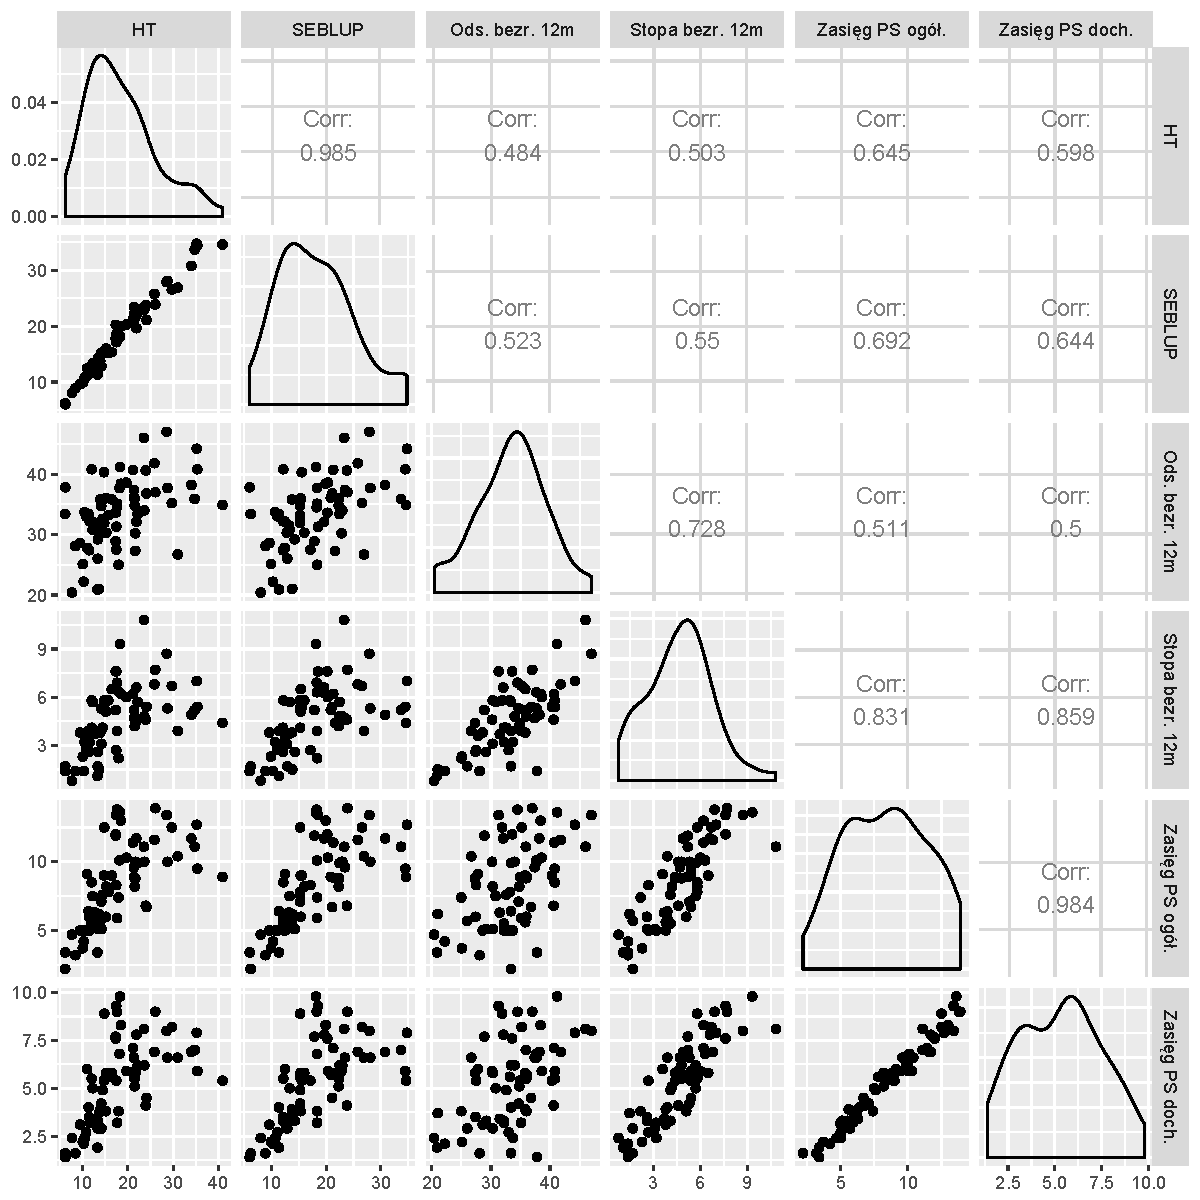
\includegraphics[width=0.8\textwidth]{05_wykresy/hcr_podreg_por-1.pdf}\\
\small{Źródło: opracowanie własne na podstawie EU-SILC 2011 oraz BDL.}
\label{fig:hcr_podreg_por}
\end{figure}

Na podstawie danych zawartych na rysunku \ref{fig:hcr_podreg_por} można zaobserwować, że oszacowania bezpośrednie i pośrednie są do siebie bardzo zbliżone. Oszacowania bezpośrednie są najsilniej skorelowane z zasięgiem korzystania ze środowiskowej pomocy społecznej ogółem ($r=0,645$). Podobnie jest w przypadku oszacowań pośrednich --- odnotowano nieznaczny wzrost wartości współczynnika korelacji do poziomu $r=0,692$. Stopa ubóstwa ekonomicznego wyznaczona z zastosowaniem estymatora SEBLUP jest przeciętnie 2,2 razy wyższa od zasięgu korzystania z pomocy społecznej. W obliczeniach przyjęto granicę ubóstwa równą 60\% mediany dochodów ekwiwalentnych, która w 2011 roku była dwukrotnie wyższa od granicy ustawowej (por. podrozdział \ref{pr:czasowy-wymiar-ubostwa}). Zależność pomiędzy stopą ubóstwa, a długotrwałym bezrobociem ma charakter umiarkowany. Wysoka korelacja istnieje także pomiędzy stopą bezrobocia długotrwałego i zasięgiem korzystania z pomocy społecznej. Należy jednak zwrócić uwagę na fakt, że współczynniki korelacji dla oszacowań pośrednich są zawsze wyższe od poziomu tych współczynników dla estymacji bezpośredniej \citep{wawrowski2016}.

W przypadku głębokości ubóstwa dokonano analogicznego porównania. W otrzymanych wynikach zaobserwowano identyczne zależności, co w przypadku stopy ubóstwa, z tą różnicą, że wartości współczynników korelacji były mniejsze. Wynika to z faktu, że głębokość ubóstwa mierzy bardzo specyficzne zjawisko (ubóstwo osób ubogich), które jest trudne w obserwacji na poziomie wskaźników społecznych. Odpowiednie korelogramy znajdują się w załączniku.

\subsection{Poziom powiatów}

Podobnie, jak w przypadku podregionów (por. \ref{pr:mer-podreg}) porównania oszacowań wskaźników ubóstwa dokonano na poziomie powiatów. W tym przypadku oszacowania pośrednie będą reprezentowane przez trzy estymatory: SEBLUP obliczony na poziomie obszaru oraz EB i MQ wykorzystujące dane jednostkowe. Wyniki porównania przedstawione są na rysunku \ref{fig:hcr_pow_por}.

\begin{figure}[ht]
\caption{Porównanie oszacowań stopy ubóstwa z danymi pochodzącymi z rejestrów administracyjnych na poziomie powiatów}
\centering
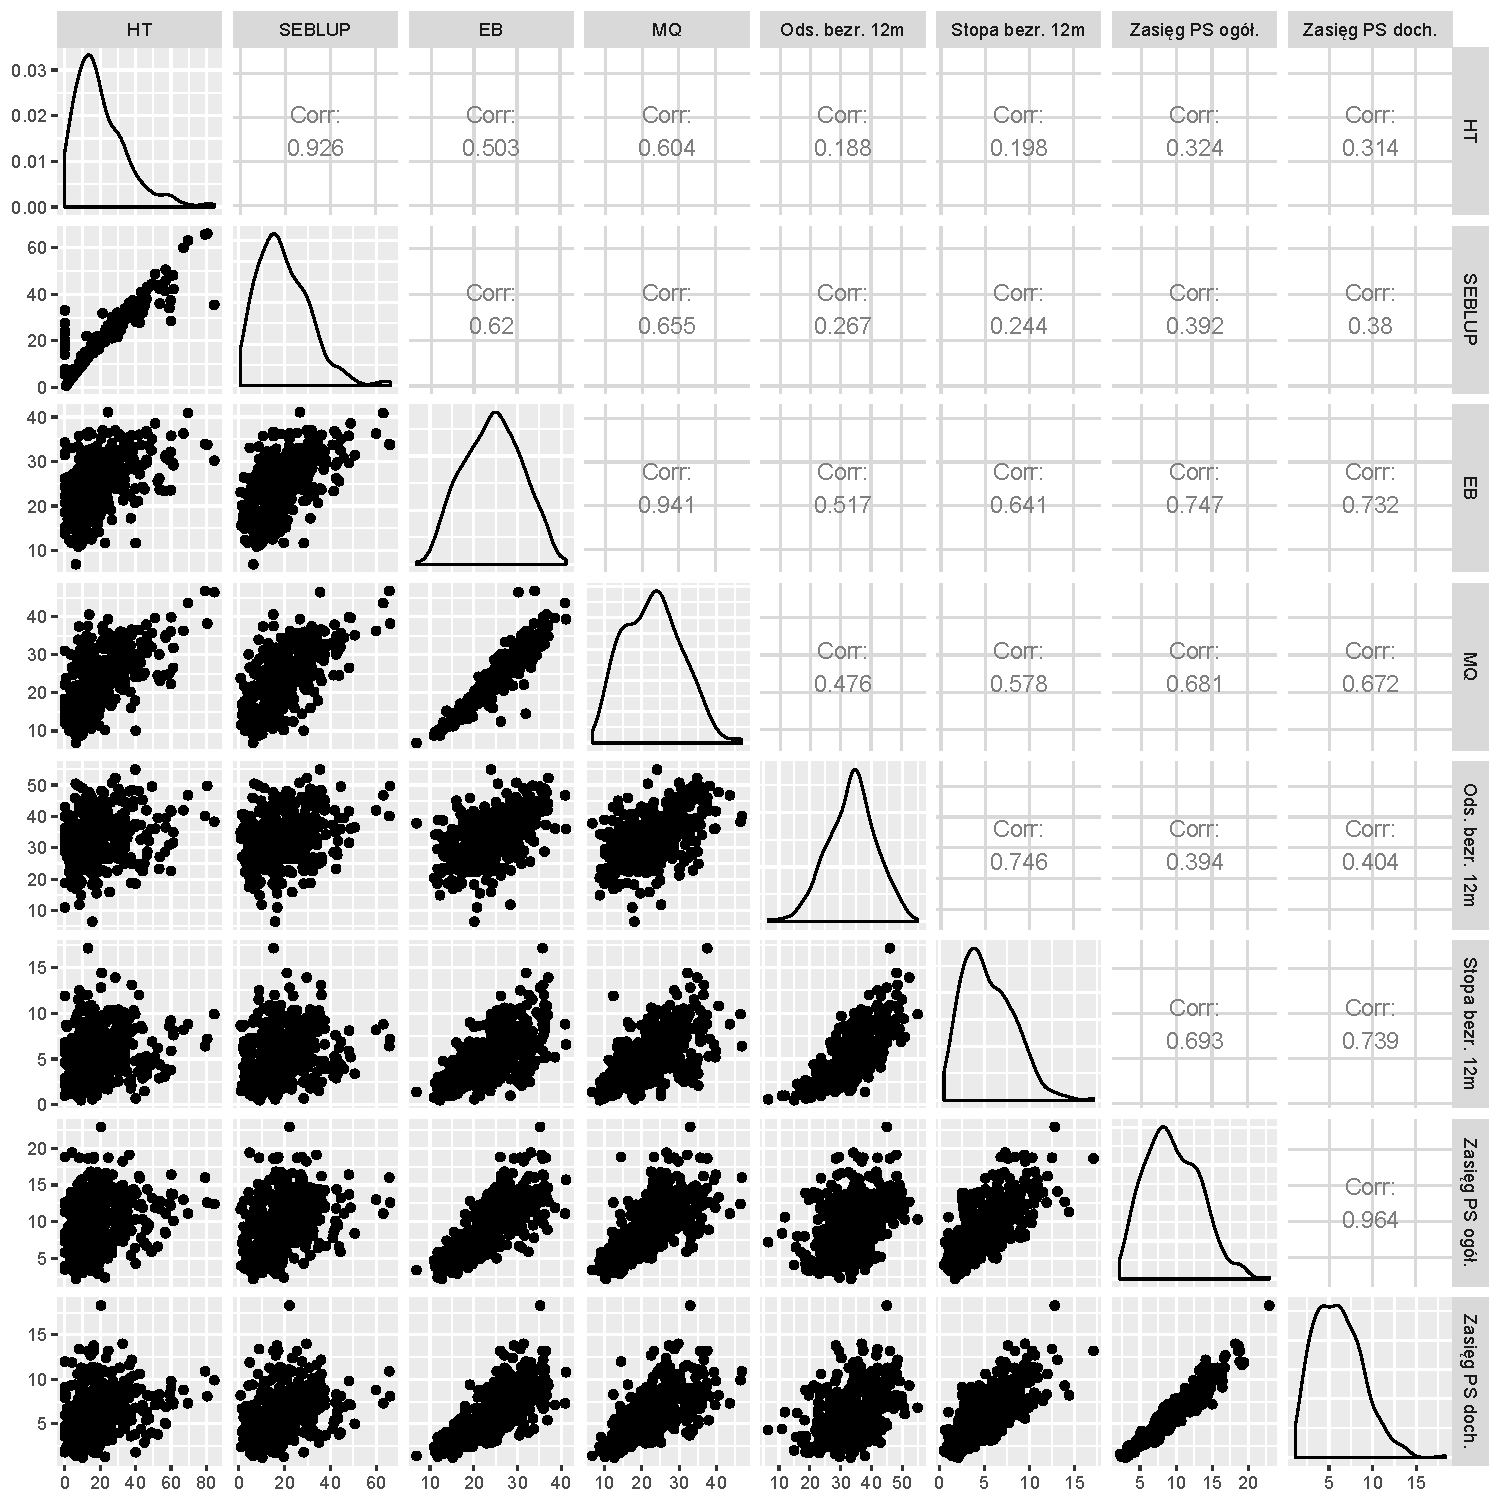
\includegraphics[width=0.8\textwidth]{05_wykresy/hcr_pow_por-1.pdf}\\
\small{Źródło: opracowanie własne na podstawie EU-SILC 2011, NSP 2011 oraz BDL.}
\label{fig:hcr_pow_por}
\end{figure}

Otrzymane zestawienie pokazuje, że oszacowania bezpośrednie są w bardzo małym stopniu skorelowane ze wskaźnikami z zakresu bezrobocia ($r=0,198$) i pomocy społecznej ($r=0,324$). Zastosowanie podejścia obszarowego w postaci estymatora SEBLUP przyczynia się do zwiększenia podobieństwa pomiędzy wartościami stopy ubóstwa oraz zmienną zasięg korzystania z~pomocy społecznej. Niemniej ta zmiana nie jest istotna (o 0,068) i nie przyczynia się do zmiany rodzaju zależności --- jest to wciąż korelacja słaba. Istotną poprawę widać natomiast w przypadku zastosowania podejścia jednostkowego --- estymatorów EB i MQ. Oszacowania otrzymane z wykorzystaniem obydwu metod są do siebie bardzo zbliżone, współczynnik korelacji liniowej Pearsona wynosi 0,941. Porównanie tych oszacowań ze stopą bezrobocia długotrwałego pokazuje istotny wzrost wartości w porównaniu do estymacji bezpośredniej. W przypadku metody EB $r=0,641$, a w przypadku metody M-kwantylowej współczynnik korelacji wynosi 0,578. Najwyższe wartości współczynników obserwuje się dla cechy: zasięg korzystania ze środowiskowej pomocy społecznej ogółem. W tym przypadku korelacja jest silna i wynosi $r=0,747$ (estymator EB) oraz $r=0,681$ (estymator MQ). Także na poziomie powiatów obserwowana jest zależność wskazująca, że pośrednie oszacowania stopy ubóstwa są średnio 2,2 razy wyższe od zasięgu korzystania z pomocy społecznej ogółem. Wartości współczynników korelacji otrzymane dla wskaźnika głębokości ubóstwa były bardzo podobne do tych, które otrzymano dla stopy ubóstwa (por. Załącznik).

Wyniki estymacji wskazują zatem, że oszacowania pośrednie uzyskane z wykorzystaniem podejścia obszarowego na poziomie podregionów oraz oszacowane na podstawie podejścia jednostkowego na poziomie powiatów w dużo większym stopniu są zbieżne z rzeczywistymi wartościami aniżeli oszacowania bezpośrednie. Większe podobieństwo pomiędzy oszacowaniami i wskaźnikami pochodzącymi z rejestrów administracyjnych stanowi argument przemawiający za stosowaniem metod statystyki małych obszarów.

\section{Wielowymiarowa analiza statystyczna poziomu ubóstwa}

W ocenie poziomu ubóstwa można także wykorzystać metody wielowymiarowej analizy statystycznej. Na podstawie oszacowań wskaźników ubóstwa uzyskanych z zastosowaniem metod estymacji pośredniej można utworzyć ranking jednostek terytorialnych --- od najmniej zagrożonych niedostatkiem do tych najbardziej narażonych na występowanie tego zjawiska. Tak uporządkowane jednostki można porównać z rankingiem podregionów czy powiatów otrzymanym na podstawie syntetycznego miernika rozwoju, który uwzględnia cechy ekonomiczno-demograficzne związane z~opisywanym zjawiskiem. Wskaźnik ten może także być wykorzystany jako zmienna niezależna w~modelu \citep{mlodak2016}.

Wykorzystując zmienne niezależne zidentyfikowane w rozdziale 4 wyznaczono syntetyczne mierniki rozwoju dla podregionów i powiatów. Następnie sprawdzano korelację rang pomiędzy oszacowaniem wskaźnika ubóstwa a miernikiem taksonomicznym. W analizie wykorzystano euklidesową miarę odległości oraz uogólnioną miarę odległości GDM \citep{Jajuga2003} dostępną w pakiecie \textit{clusterSim} \citep{clustersim2017}.

\subsection{Poziom podregionów}

W modelu zbudowanym na poziomie podregionów objaśniającym stopę ubóstwa znalazły się cztery zmienne niezależne (por. podrozdział \ref{pr:model-podreg}). Na podstawie znaków stojących przy parametrach $\beta$ określono charakter cechy jako stymulantę (S) lub destymulantę (D). Wśród zmiennych diagnostycznych danego wskaźnika ubóstwa znalazły się:

\begin{itemize}
\item dla stopy ubóstwa
\begin{itemize}
\item udział rodzin z 3 dzieci poniżej 24 roku życia pozostających na utrzymaniu w liczbie rodzin z dziećmi poniżej 24 roku życia (S), 
\item odsetek mieszkań posiadających ustęp spłukiwany (D),
\item udział osób niepełnosprawnych prawnie w liczbie ludności ogółem (S),
\item gęstość zaludnienia (S);
\end{itemize}
\item dla głębokości ubóstwa
\begin{itemize}
\item udział dzieci w wieku do lat 17, na które rodzice otrzymują zasiłek rodzinny w ogólnej liczbie dzieci w tym wieku (S), 
\item udział osób w wieku 20--29 lat pozostających na utrzymaniu w ogólnej liczbie osób w~wieku 20-29 lat (S), 
\item udział mieszkań, gdzie przypada powyżej 3 osób na izbę w ogólnej liczbie mieszkań (S), 
\item przeciętna liczba osób w gospodarstwie domowym (D) 
\item stopa bezrobocia rejestrowanego osób pozostających bez pracy powyżej 12 miesięcy (D).
\end{itemize}
\end{itemize}

W celu wyznaczenia wartości syntetycznego miernika rozwoju w pierwszej kolejności dokonano ujednolicenia charakteru zmiennych oraz zastosowano standaryzację w celu pozbawienia wartości cech mian. Jako obiekt wzorcowy wybrano dolny biegun rozwoju --- w założeniu jednostkę o~najniższych wartościach zmiennych diagnostycznych i najwyższym poziomie ubóstwa.

Współczynnik korelacji rang Spearmana pomiędzy uogólnioną miarą odległości GDM a oszacowaniami pośrednimi stopy ubóstwa wyniósł $r_S=0,8764$. Zastosowanie odległości euklidesowej skutkuje korelacją na poziomie $r_S=0,8555$, a więc nieznacznie niższą. W przypadku porównania odległości i bezpośredniego oszacowania wskaźnika zasięgu ubóstwa otrzymana korelacja była równa $r_S=0,8176$ dla miary GDM i $r_S=0,7943$ dla odległości euklidesowej. Podobnie jak w przypadku \textit{zmiennych proxy}, także tutaj widoczna była poprawa współczynnika korelacji na korzyść oszacowań pośrednich.

Analogiczna analiza korelacji przeprowadzona dla głębokości ubóstwa charakteryzuje się występowaniem znacznie słabszych zależności. Współczynnik korelacji rang Spearmana pomiędzy oszacowaniem wskaźnika głębokości ubóstwa i miarą GDM wynosił $r_S=0,4699$, a dla miary euklidesowej $r_S=0,3517$. 

Na rysunku \ref{fig:podreg-gdm} przedstawiono porównanie rankingu otrzymanego na podstawie oszacowań estymatora SEBLUP oraz miary GDM. Pierwsze miejsce zajmuje podregion o najniższym wskaźniku ubóstwa. 

\begin{figure}[ht]
\caption{Porównanie rankingów uzyskanych na podstawie estymacji pośredniej oraz miary GDM na poziomie podregionów}
\centering
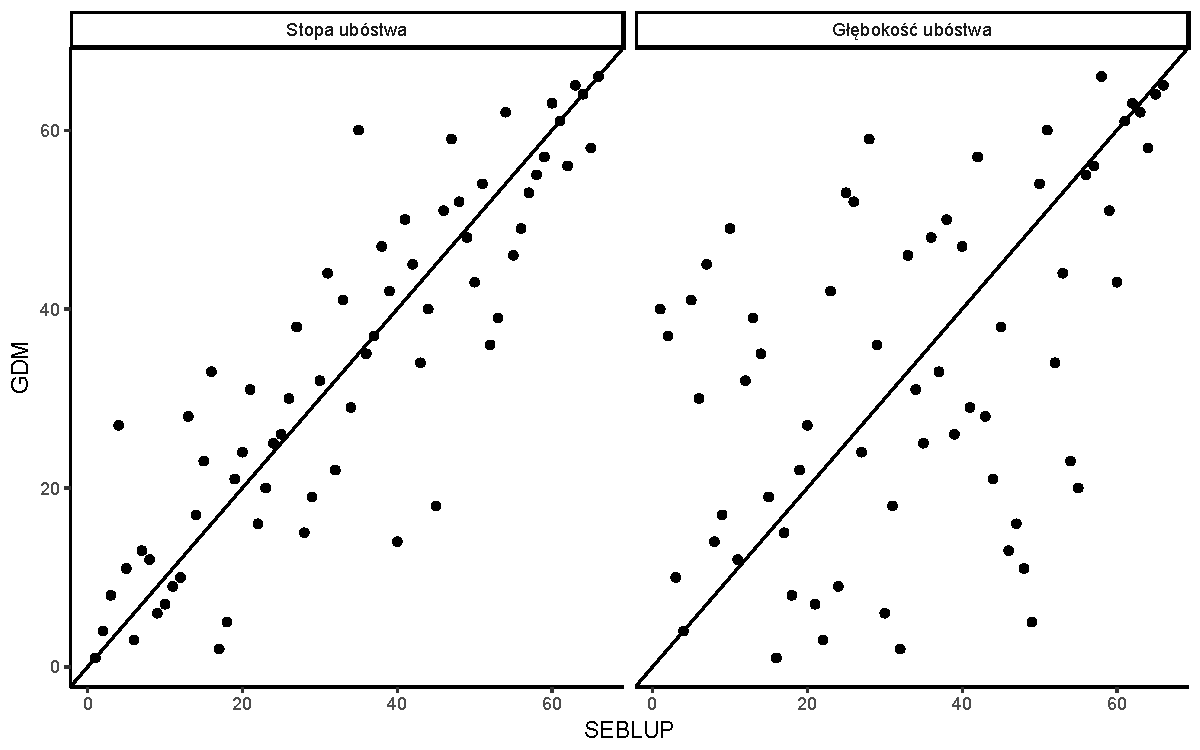
\includegraphics[width=\textwidth]{05_wykresy/podreg_gdm-1.pdf}\\
\small{Źródło: opracowanie własne na podstawie EU-SILC 2011 oraz BDL.}
\label{fig:podreg-gdm}
\end{figure}

W przypadku stopy ubóstwa te same miejsca w rankingu bez względu na zastosowaną metodę zajęły 4 podregiony --- m. Warszawa (1), podregion krakowski (37), nowosądecki (61) i puławski (64). Największy spadek w rankingu w odniesieniu do estymacji pośredniej zanotowano dla podregionu elbląskiego --- 35 miejsce według estymatora SEBLUP i 60 według miary GDM oraz miasta Kraków z 4 lokaty na 27. Z kolei największą poprawę zaobserwowano dla podregionu bytomskiego --- 35 lokata na podstawie oszacowania pośredniego i 18 miejsce na podstawie miary GDM. Drugim podregionem o równie dużej zmianie w klasyfikacji był podregion koszaliński (z 40 pozycji na 14).

Pogrupowanie obserwowanych różnic w rankingach w grupy o szerokości 10 pozycji pokazuje, że dla stopy ubóstwa w 78,8\% różnice te nie były większe niż 10 miejsc. W przedziale $(10;20]$ odnotowano 10 podregionów, natomiast zidentyfikowano tylko cztery podregiony o największym odchyleniu. W przypadku głębokości ubóstwa frakcje podregionów w poszczególnych przedziałach różnią się od tych dla zasięgu ubóstwa. W pierwszym przedziale znalazło się 45,5\% wszystkich podregionów, a w drugim 24,2\%. Pozostałe 20 podregionów charakteryzuje się różnicami przekraczającymi 20 miejsc.

% Swoje miejsca w rankingu dla głębokości ubóstwa zachowały podregiony poznański (4) oraz bialski (61). 

\subsection{Poziom powiatów}

Na poziomie powiatów ranking według poziomu ubóstwa utworzono na podstawie rezultatów otrzymanych metodą EB. Z racji tego, że dane wejściowe do tego podejścia były mierzono na poziomie gospodarstw domowych, dokonano agregacji zmiennych użytych w modelu do poziomu powiatów. Podstawą obliczeń były następujące cechy:

\begin{itemize}
\item odsetek mężczyzn w powiecie (S),
\item odsetek osób w wieku 30-44 w powiecie (S),
\item odsetek osób w wieku 65 lat i więcej w powiecie (D),
\item odsetek osób bezrobotnych w powiecie (D),
\item odsetek osób niepełnosprawnych w powiecie (D),
\item odsetek osób z wykształceniem podstawowym w powiecie (D),
\item odsetek osób z wykształceniem wyższym w powiecie (S),
\item wskaźnik obciążenia demograficznego dzieci w powiecie (D),
\item odsetek gospodarstw posiadających 1 pokój (D)
\item odsetek gospodarstw posiadających 3 pokoje i więcej (S),
\item odsetek osób zamieszkałych na wsi lub w mieście do 20 tys. osób (D),
\item stopa bezrobocia rejestrowanego (D),
\item odsetek osób zatrudnionych w rolnictwie (D),
\item wypłacone świadczenie społeczne na 1000 zatrudnionych osób (D).
\end{itemize}

Dla tak zdefiniowanego zestawu zmiennych diagnostycznych wyznaczono miarę odległości GDM oraz odległość euklidesową. Współczynnik korelacji rang Spearmana pomiędzy miarą GDM a pośrednimi oszacowaniami stopy ubóstwa był wysoki i wynosił $r_S=0,7423$. Uwzględnienie odległości euklidesowej spowodowało spadek tego współczynnika do poziomu $r_S=0,6999$. Zależność pomiędzy syntetyczną miarą rozwoju a oszacowaniami bezpośrednimi była słaba --- $r_S=0,3470$ dla miary GDM i $r_S=0,3472$ dla odległości Euklidesa. Korelacje dla wskaźnika głębokości ubóstwa były na bardzo zbliżonym poziomie.

Na rysunku \ref{fig:jedn-gdm} przedstawiono porównanie rankingu utworzonego na podstawie metody EB i~miary GDM.

\begin{figure}[ht]
\caption{Porównanie rankingów uzyskanych na podstawie estymacji pośredniej oraz miary GDM na poziomie powiatów}
\centering
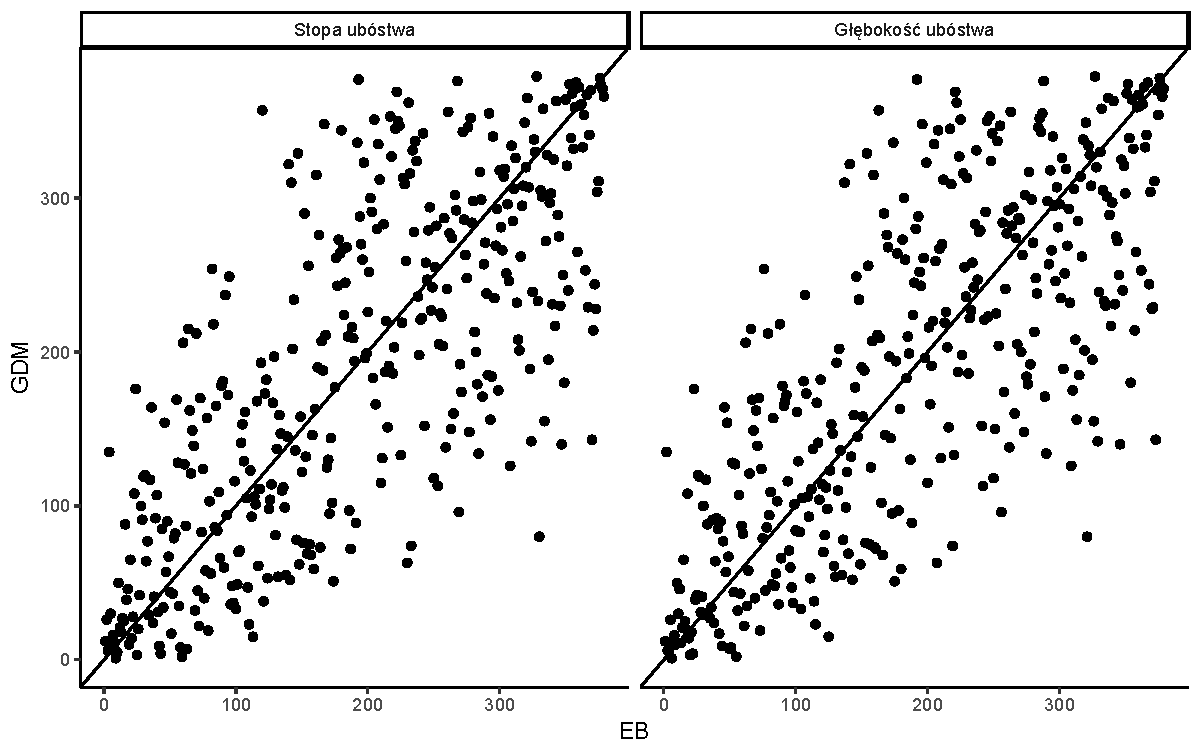
\includegraphics[width=\textwidth]{05_wykresy/jedn_gdm-1.pdf}\\
\small{Źródło: opracowanie własne na podstawie EU-SILC 2011, NSP 2011 oraz BDL.}
\label{fig:jedn-gdm}
\end{figure}

Powiaty na początku i końcu rankingu grupują się wokół prostej $y=x$, co pozwala stwierdzić, że dla tych jednostek nie występują znaczne przesunięcia. Niemniej tylko w przypadku dwóch powiatów dla stopy ubóstwa miejsca w obu rankingach pokrywają się. Są to powiaty brodnicki i pińczowski. Także dla głębokości ubóstwa z taką sytuacją mamy do czynienia tylko w dwóch jednostkach --- powiatach zgierskim i lipnowskim. Na uwagę zasługuje zmiana w klasyfikacji miasta Sopot. Powiat zajmujący 4 miejsce według poziomu zasięgu ubóstwa oraz 2 miejsce pod względem głębokości ubóstwa zajmuje 135 miejsce na podstawie rankingu GDM. 

Pogrupowanie różnic pomiędzy pozycją w rankingu według wartości wskaźnika ubóstwa oraz miary GDM w przedziały o szerokości 20 jednostek umożliwia ocenę skali zmian. W przypadku stopy ubóstwa różnica w obrębie 20 pozycji dotyczyła 100 powiatów, które stanowią 26,4\% wszystkich analizowanych jednostek. W kolejnych klasach obserwacji jest coraz mniej --- w przedziale różnic $(20;40]$ znalazło się już 19,5\% powiatów, a w kolejnym 10,8\%. Wzrost obserwowany jest dopiero dla przedziału 100 i więcej --- 20,1\% liczby powiatów. Bardzo zbliżony rozkład różnic pomiędzy pozycjami w rankingach obserwowany jest dla wskaźnika głębokości ubóstwa. 

\section{Identyfikacja i opis enklaw ubóstwa}

Na podstawie analizy przeprowadzonej w pierwszej części rozdziału jako oszacowania wskaźników ubóstwa wybrano oceny parametrów otrzymane na podstawie estymatora SEBLUP dla poziomu podregionów oraz estymatora EB dla poziomu powiatów. Opierając się na wartościach tych oszacowań utworzono kartogramy, które stały się podstawą do przeprowadzenia analizy terytorialnego zróżnicowania ubóstwa. Na rysunkach przedstawione są oszacowania stopy oraz głębokości ubóstwa w ujęciu przestrzennym.

\subsection{Poziom podregionów}

Rysunek \ref{fig:fh_nts3_hcr_pgi_4} przedstawia wartości stopy oraz głębokości ubóstwa w układzie 66 podregionów. Wartości wskaźników ubóstwa zostały pogrupowane w 4 przedziały klasowe.

\begin{figure}[ht]
\caption{Terytorialne zróżnicowanie stopy oraz głębokości ubóstwa w przekroju podregionów w 2011 roku}
\centering
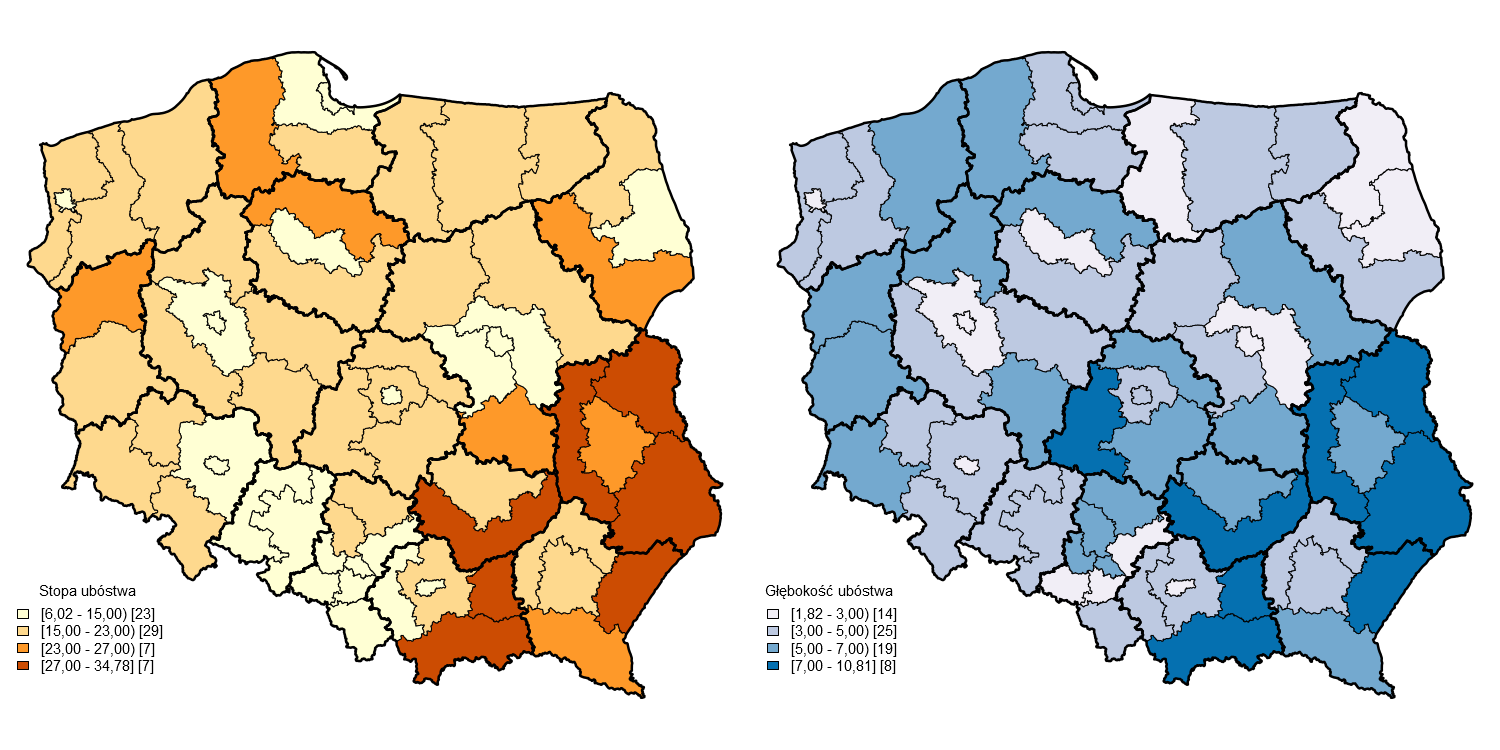
\includegraphics[width=\textwidth]{05_wykresy/fh_nts3_hcr_pgi_4.png}\\
\small{Źródło: opracowanie własne na podstawie EU-SILC 2011 oraz BDL.}
\label{fig:fh_nts3_hcr_pgi_4}
\end{figure}

Najwyższe wartości stopy ubóstwa obserwowane są w południowo-wschodniej części Polski. Są to podregiony: bialski, tarnowski, puławski, chełmsko-zamojski, sandomiersko-jędrzejowski, nowosądecki oraz przemyski. Te podregiony należą do tzw. Polski ,,B'', której w przeszłości domeną rozwoju było rolnictwo. Program Operacyjny Rozwój Polski Wschodniej realizowany ze środków UE w latach 2007--2013 miał na celu wyrównanie istniejących różnic. Z kolei najniższy poziom niedostatku obserwowany jest w podregionach, które równocześnie są miastami na prawach powiatu --- m. Warszawa, m. Wrocław, m. Poznań oraz m. Kraków. Kolejne miejsca rankingu zajmują podregiony, które częściowo tworzą konurbację górnośląską czyli podregion sosnowiecki, rybnicki, tyski oraz bielski. Wyraźnie widoczny jest wpływ dużych miast na poziom ubóstwa w ich sąsiedztwie. Przykładem może tu być m. Poznań oraz podregion poznański, m. Wrocław oraz podregion wrocławski czy podregion trójmiejski i gdański. Podregiony, które zawierają ważne ośrodki miejskie również charakteryzują się niższą stopą ubóstwa --- podregion bydgosko-toruński, podregion rzeszowski tudzież podregion białostocki.

W przypadku drugiej analizowanej cechy --- głębokości ubóstwa, najmniejsza luka dochodowa wśród osób żyjących poniżej linii ubóstwa obserwowana jest w podregionach m. Warszawa, m.~Wrocław, m. Poznań, białostockim oraz poznańskim. Największe ubóstwo ubogich występuję w~tych samych podregionach, w których zidentyfikowano także najwyższe wartości stopy ubóstwa. Podregion suwalski jest przykładem obszaru, który charakteryzuje się dosyć wysoką stopą ubóstwa --- 19,9\%, a równocześnie niskim poziomem ubóstwa osób ubogich --- 2,6\%. Na rysunku \ref{fig:fh_nts3_hcr_pgi_4} wyróżnia się podregion sieradzki w województwie łódzkim, który znajduje się w przedziale klasowym o najwyższej głębokości ubóstwa, natomiast wartość stopy ubóstwa jest na poziomie całego województwa. Jest to przykład niedoskonałości narzędzia prezentacji, jakim jest mapa o sztywno ustalonych przedziałach klasowych. W podregionie sieradzkim stopa ubóstwa wynosi 22,4\% czyli bliżej górnej granicy przedziału klasowego, a głębokość ubóstwa 7\% czyli na granicy przedziału klasowego.

Uzupełnieniem analizy była klasyfikacja wartości wskaźników ubóstwa do 3 grup metodą k-średnich. W tym celu zastosowano funkcję \textit{classIntervals} z pakietu \textit{classInt} \citep{classint2015}.

\begin{figure}[ht]
\caption{Klasyfikacja stopy oraz głębokości ubóstwa w przekroju podregionów w 2011 roku}
\centering
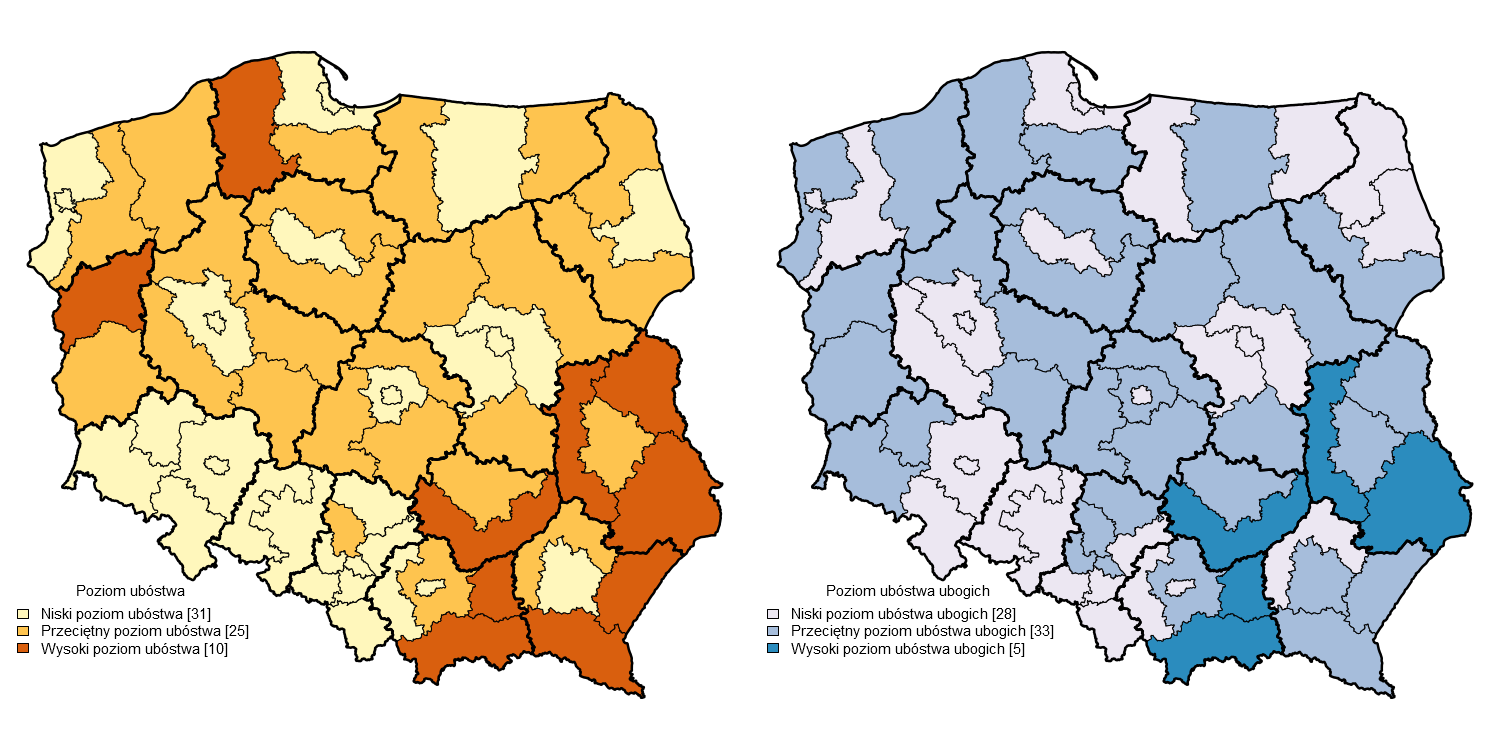
\includegraphics[width=\textwidth]{05_wykresy/fh_nts3_hcr_pgi_k3.png}\\
\small{Źródło: opracowanie własne na podstawie EU-SILC 2011 oraz BDL.}
\label{fig:fh_nts3_hcr_pgi_k3}
\end{figure}

Przeprowadzona klasyfikacja pozwoliła na wyróżnienie enklaw charakteryzujących się występowaniem niskiego, przeciętnego oraz wysokiego poziomu ubóstwa oraz ubóstwa osób ubogich. Podregionów charakteryzujących się niskim poziomem ubóstwa jest 31. W tej klasie znajdują się podregiony o wartościach stopy ubóstwa nieprzekraczającej 16,6\%. Do tej grupy zaklasyfikowano podregiony będące miastami oraz zawierające duże ośrodki miejskie. Cały obszar Śląska został także zaklasyfikowany do tej grupy za wyjątkiem podregionu bytowskiego. Wysoki poziom ubóstwa występuje w podregionach Polski południowo-wschodniej --- w województwach małopolskim, podkarpackim, lubelskim, świętokrzyskim. Ponadto do tej grupy przynależą dwa podregiony leżące w północnej części kraju --- słupski i gorzowski. Wartością, która determinowała zaklasyfikowanie do klasy o wysokim poziomie ubóstwa było oszacowanie stopy ubóstwa powyżej 24,8\%. 

Podobnie jak w przypadku stopy ubóstwa niski poziom ubóstwa ubogich odnotowuje się głównie w ośrodkach miejskich. Pierwszą grupę stanowią podregiony, w których oszacowane głębokości ubóstwa nie przekraczało 4,2\%. Do grupy obszarów o wysokim poziomie ubóstwa osób ubogich zaklasyfikowano 5 podregionów znajdujących się w południowo-wschodniej części kraju. Głębokość ubóstwa w tych podregionach była wyższa od 7,6\%.

Uzyskane wyniki przeanalizowano także pod katem spójności przestrzennej. W tym celu wyznaczono statystykę Morana I dla stopy i głębokości ubóstwa wykorzystując macierz sąsiedztwa podregionów. Obliczone wartości statystyki wykazały istnienie dodatniej autokorelacji oszacowań. Wartość statystyki dla stopy ubóstwa była równa 0,47, a dla głębokości ubóstwa 0,37 i była istotna statystycznie. 

%Obliczenia przeprowadzono funkcją \textit{moran.test} z pakietu \textit{spdep} 

\subsection{Poziom powiatów}

Specyfika podziału terytorialnego Polski powoduje, że kolejny poziom estymacji charakteryzuje się prawie sześciokrotnym wzrostem liczby domen. Na rysunku \ref{fig:eb_nts4_hcr_pgi_7} przedstawiono wartości stopy i głębokości ubóstwa dla powiatów. Z racji większej liczby jednostek oraz większej rozpiętości oszacowań zastosowano 7-stopniową skalę barw. 

\begin{figure}[ht]
\caption{Terytorialne zróżnicowanie stopy oraz głębokości ubóstwa w przekroju powiatów w 2011 roku}
\centering
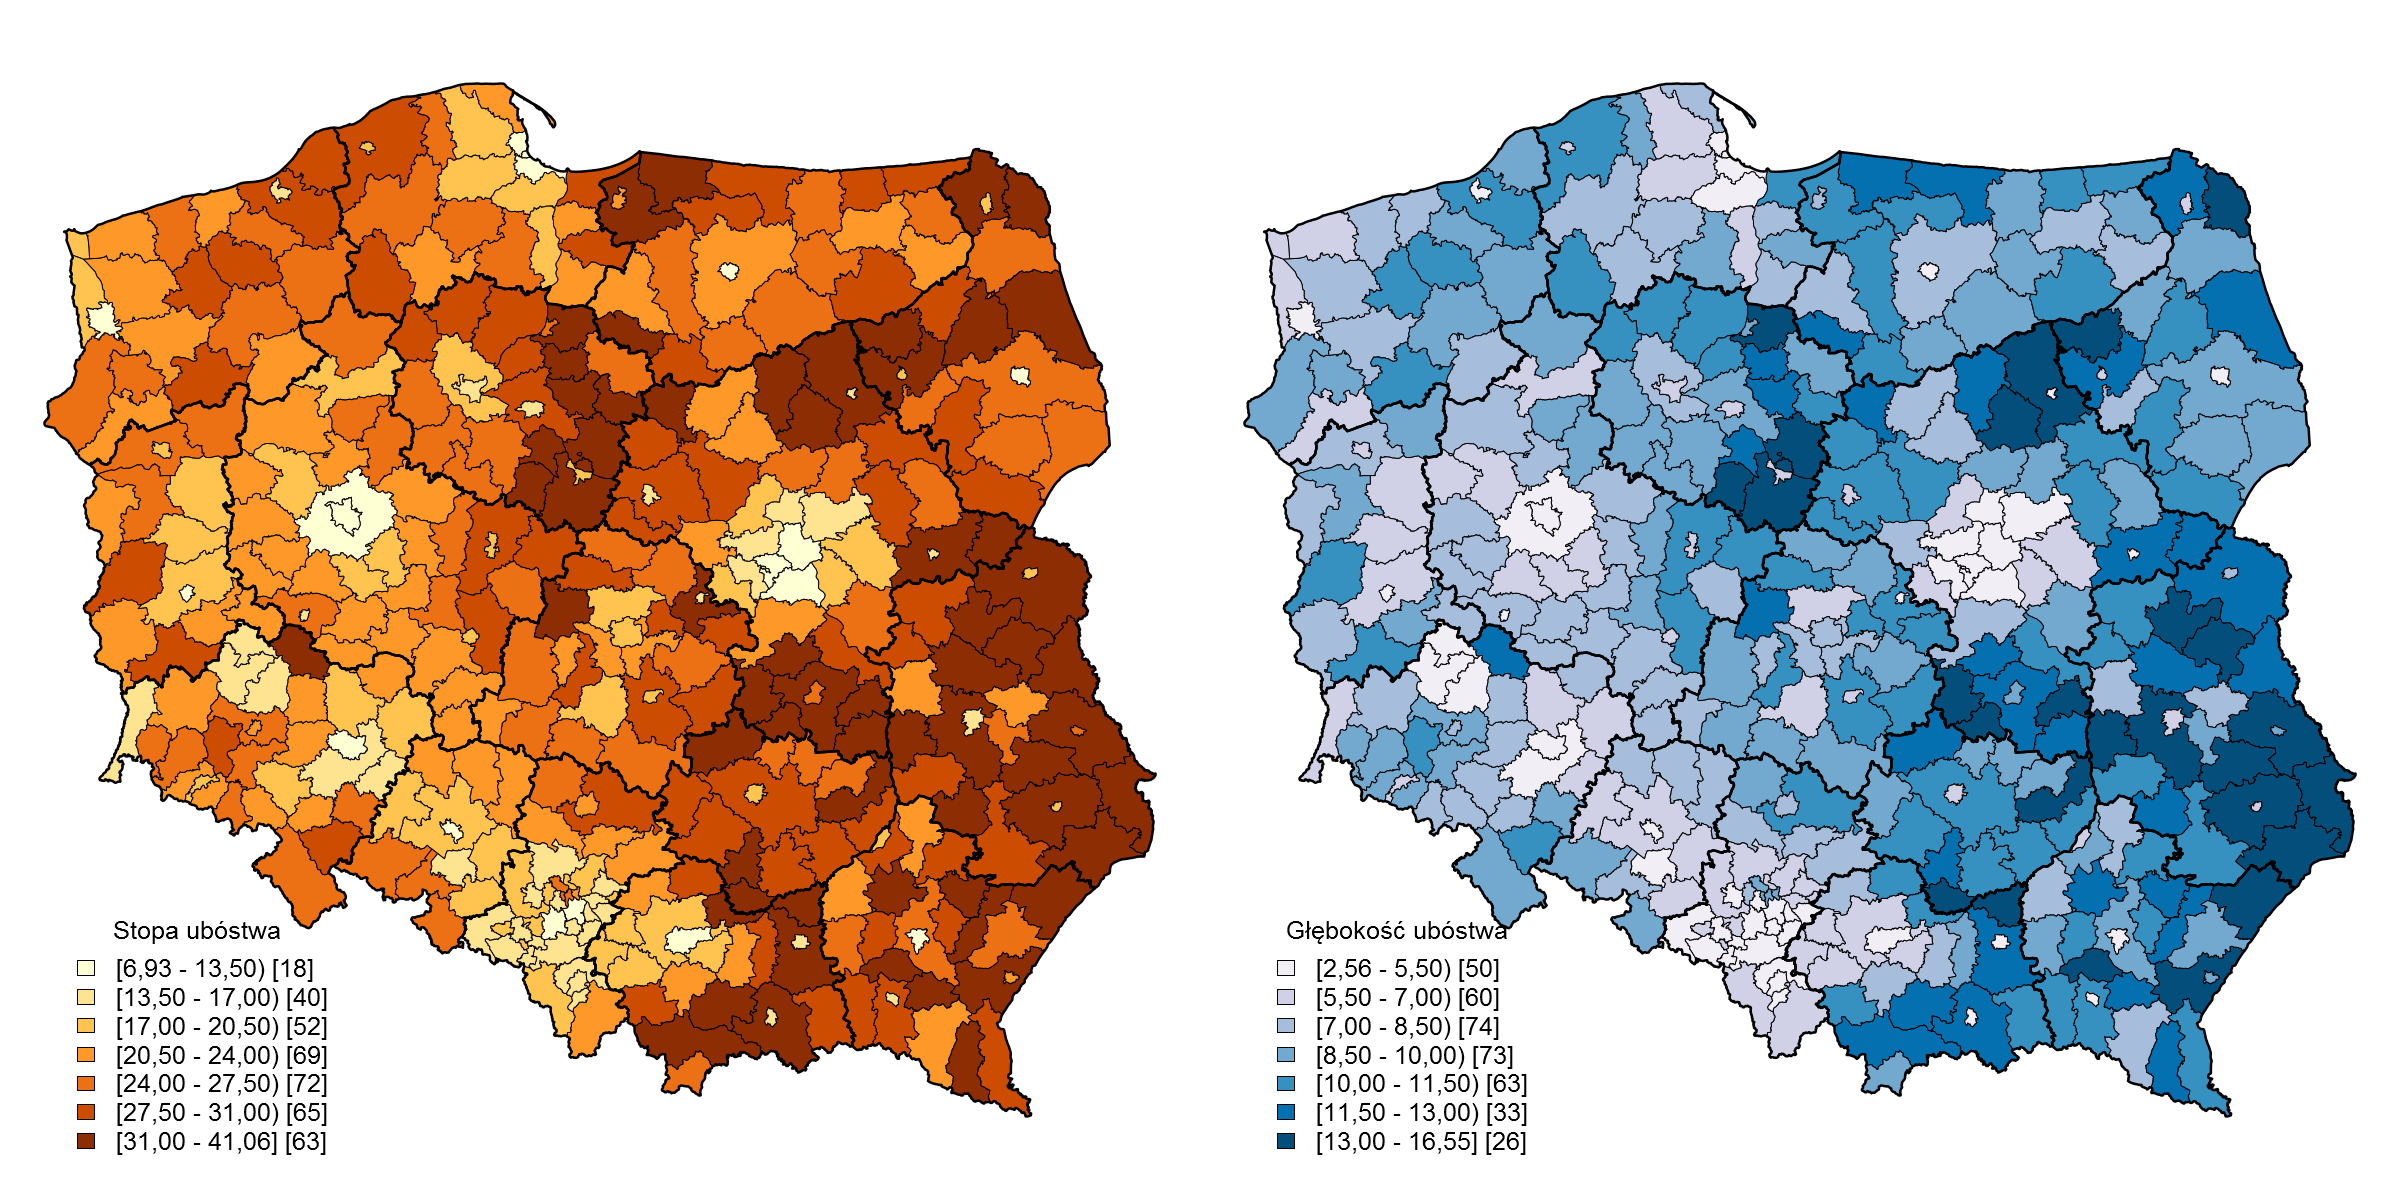
\includegraphics[width=\textwidth]{05_wykresy/eb_nts4_hcr_pgi_7.png}\\
\small{Źródło: opracowanie własne na podstawie EU-SILC 2011, NSP 2011 oraz BDL.}
\label{fig:eb_nts4_hcr_pgi_7}
\end{figure}

Najwyższe wartości stopy ubóstwa są obserwowane w powiatach znajdujących się we wschodniej części kraju oraz jednostkach znajdujących się w znacznej odległości od stolic województw. Występowaniem największego ubóstwa --- powyżej 40\% --- charakteryzuje się powiat chełmski (41,1\%) oraz hrubieszowski (40,9\%). Wśród 20 powiatów o najwyższych wartościach stopy ubóstwa znajdują się trzy powiaty położone we wschodniej części województwa kujawsko-pomorskiego, pięć powiatów województwa lubelskiego oraz jeden powiat znajdujący się w województwie małopolskim (powiat dąbrowski). Aż pięć powiatów pochodzi z województwa mazowieckiego, przy czym są to powiaty znacznie oddalone od miasta stołecznego Warszawa: ostrołęcki i makowski (znajdujące się w północnej części województwa) oraz przysuski, szydłowiecki i zwoleński (umiejscowione w południowej części województwa). Wśród tych dwudziestu jednostek po dwie pochodzą z województwa podkarpackiego, podlaskiego i świętokrzyskiego.

Najniższe wartości stopy ubóstwa to miasta na prawach powiatu oraz powiaty bezpośrednio z nimi sąsiadujące. Na pierwszym miejscu jest m. st. Warszawa (6,9\%), na drugim m. Poznań (10,9\%), a na trzecim, graniczący z Warszawą powiat pruszkowski (11,2\%). Dalsze pozycje rankingu zajmują miasta na prawach powiatu: m. Gdynia, m. Sopot (po 11,7\%), m. Opole, m. Rzeszów, m. Olsztyn (po 12,8\%). Wśród 20 powiatów o najniższej stopie ubóstwa znajdują się wyłącznie miasta na prawach powiatu oraz jednostki bezpośrednio graniczące z tymi powiatami.

W przypadku wartości luki dochodowej obserwowana jest wysoka korelacji tej cechy ze stopą ubóstwa ($r=0,99$). Najmniejsze ubóstwo wśród osób ubogich obserwowane jest w Warszawie (2,6\%) Na kolejnych miejscach znajdują się: powiat pruszkowski i miasto Sopot (po 3,8\%) oraz powiat poznański i miasto Poznań (po 3,9\%). Najwyższe oszacowania wskaźnika głębokości ubóstwa odnotowano w tych samych powiatach, w których występowała wysoka stopa ubóstwa. 

Na podstawie wartości wskaźników ubóstwa, na poziomie powiatów także dokonano klasyfikacji, tym razem tworząc 5 grup poziomu ubóstwa. Wyniki klasyfikacji przedstawione są na rysunku \ref{fig:eb_nts4_hcr_pgi_k5}.

\begin{figure}[ht]
\caption{Klasyfikacja stopy oraz głębokości ubóstwa w przekroju powiatów w 2011 roku}
\centering
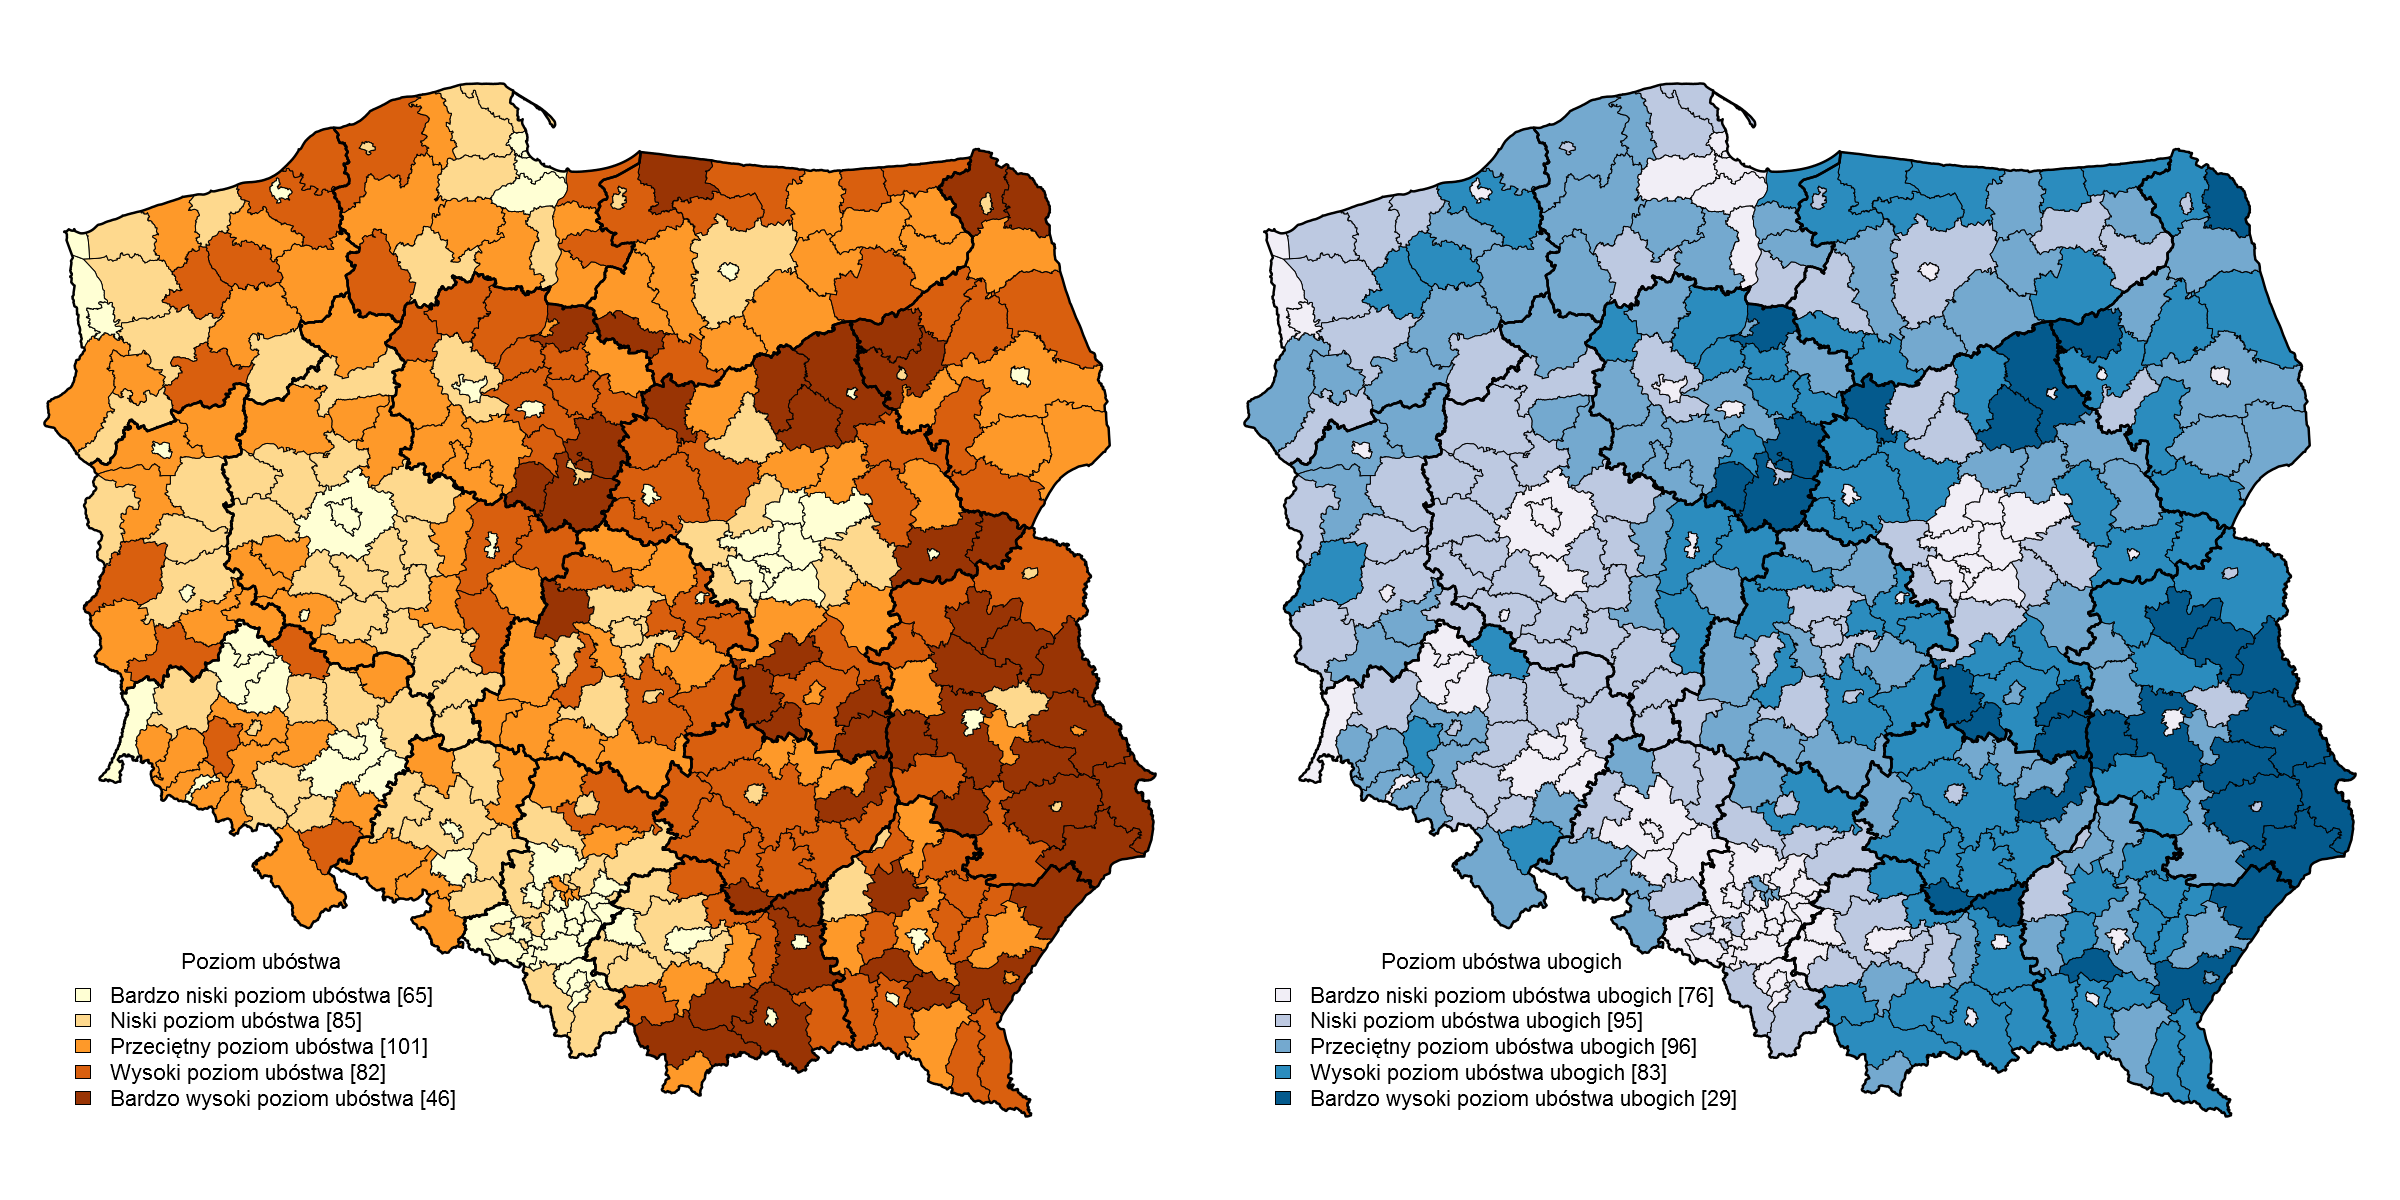
\includegraphics[width=\textwidth]{05_wykresy/eb_nts4_hcr_pgi_k5.png}\\
\small{Źródło: opracowanie własne na podstawie EU-SILC 2011, NSP 2011 oraz BDL.}
\label{fig:eb_nts4_hcr_pgi_k5}
\end{figure}

W przypadku powiatów wyróżniono 5 poziomów ubóstwa. Do grupy o bardzo niskim poziomie ubóstwa zaklasyfikowano 65 powiatów. Tyle wynosi liczba miast na prawach powiatu w Polsce, ale w tej grupy nie znalazły się wszystkie z nich. Granicą przynależności do tych powiatów była wartość wskaźnika stopy ubóstwa poniżej 17,4\%. Najwięcej powiatów znalazło się w grupie cechującej się przeciętnym poziomem ubóstwa --- 27\% wszystkich powiatów o wartościach zasięgu ubóstwa z przedziału $[22,7\% -- 27,4\%]$. Do klasy powiatów o bardzo wysokim poziomie ubóstwa (powyżej 32,4\%) włączono 46 jednostek znajdujących się przede wszystkim we wschodniej części Polski. Łącznie w kategoriach zawierających powiaty o bardzo niskim oraz niskim poziomie ubóstwa znalazło się 150 jednostek administracyjnych, a w grupach wysokiego i bardzo wysokiego poziomu ubóstwa 128 powiatów. 

Analiza klas wyłonionych dla wskaźnika głębokości ubóstwa wskazuje, że ubóstwo osób ubogich nie jest bardzo wysokie. Powiatów o bardzo niskim poziomie ubóstwa ubogich jest 76 --- o 11 więcej, w porównaniu do tej samej klasy opisującej stopę ubóstwa. W tej grupie znalazły się powiaty charakteryzujące się głębokością ubóstwa mniejszą niż 6,2\%. Przeciętna wartość luki dochodowej zawiera się w przedziale $[8,2\% -- 10,2\%]$ i jest charakterystyczna dla 96 powiatów. Jednostek o bardzo wysokim ubóstwie osób żyjących poniżej granicy niedostatku jest zaledwie 29. W tej grupie wskaźnik głębokości ubóstwa przekracza 12,6\%. Także w przypadku tego wskaźnika obserwowana jest wyraźna przewaga liczby powiatów w grupach poniżej przeciętnych wartości (171 domen) w porównaniu do liczby powiatów o wysokim i bardzo wysokim poziomie ubóstwa osób ubogich (112).

Na podstawie wartości wskaźników ubóstwa oszacowanych na szczeblu powiatowym oraz macierzy sąsiedztwa obliczono także statystykę Morana I. Podobnie jak w przypadku poziomu podregionów, także na tym poziomie terytorialnym odnotowano istnienie dodatniej korelacji przestrzennej --- statystyka wynosiła odpowiednio 0,45 dla stopy i 0,47 dla głębokości ubóstwa. 

\section{Podsumowanie}

Celem działań przeprowadzonych w rozdziale piątym była analiza wskaźników ubóstwa oszacowanych z wykorzystaniem metod statystyki małych obszarów, która uwzględniała zarówno ocenę dotyczącą wykorzystanych metod, jak i wymiar przestrzenny. Dane statystyczne, które zawierałyby informację o stopie oraz głębokości ubóstwa w populacji nie są nigdzie publikowane, w~związku z czym weryfikacja uzyskanych szacunków pośrednich bazowała na porównaniu z cechami mogącymi przybliżyć dane zjawisko, tzw. \textit{zmiennymi proxy}. Po gruntownej analizie dostępnych źródeł danych zdecydowano się na odwołanie się do informacji pochodzących z rejestrów administracyjnych, które dotyczyły bezrobocia rejestrowanego oraz korzystania z pomocy społecznej. Wykazano, że oszacowania pośrednie są silniej skorelowane ze wskaźnikami bezrobocia długotrwałego oraz korzystania z pomocy społecznej, aniżeli te, oszacowane z zastosowaniem estymatora bezpośredniego. 

Jako narzędzie oceny oszacowań pośrednich zaproponowano metody wielowymiarowej analizy statystycznej, a dokładnie syntetyczny miernik rozwoju. Wyznaczenie rankingu dla podregionów i powiatów bazowało na zmiennych niezależnych zidentyfikowanych jako zmienne pomocnicze w~modelach obszarowych oraz jednostkowych wypracowanych w rozdziale 4. Na podstawie tak określonego zestawu cech diagnostycznych wyznaczono odległość euklidesową oraz GDM od obiektu wzorcowego. Porównanie współczynników korelacji rang Spearmana oszacowań pośrednich wskaźników ubóstwa oraz syntetycznych mierników rozwoju wykazało istnienie silnej dodatniej zależności pomiędzy rankingiem uzyskanym na podstawie wartości zasięgu ubóstwa, a miarą odległości GDM. Zależność ta była słabsza w przypadku zastosowania euklidesowej miary odległości. Wyniki przeprowadzonej analizy świadczą o tym, że miara odległości GDM może stanowić narzędzie merytorycznej oceny oszacowań wskaźników ubóstwa oraz może służyć do wykrywania wartości nietypowych.

W ostatniej części rozdziału dokonano przestrzennej oceny wskaźników ubóstwa oszacowanych z wykorzystaniem metod estymacji pośredniej. Zidentyfikowano obszary, znajdujące się głównie we wschodniej części Polski, charakteryzujące się wysokim poziomem ubóstwa. Jednostkami, które cechują się niskim ubóstwem są przede wszystkim duże miasta oraz powiaty je okalające. Wraz ze wzrostem odległości do najbliższego dużego ośrodka miejskiego rośnie także poziom niedostatku. Obserwuje się także niskie ubóstwo na terenie praktycznie całego Śląska, co może być uzasadnione istnieniem autostrady A4 łączącej wszystkie większe ośrodki miejskie na tym terenie. Pomiędzy oszacowaniami wskaźników ubóstwa istnieje umiarkowana dodatnia autokorelacja przestrzenna świadcząca o podobieństwie wartości sąsiadujących.

\chapter*{Zakończenie}
\addcontentsline{toc}{chapter}{Zakończenie}
W rozprawie podjęto aktualną i ważką tematykę ubóstwa w kontekście estymacji dla małych domen. Przeprowadzone badania empiryczne umożliwiły realizację głównego celu pracy jakim był pomiar ubóstwa na poziomie podregionów i powiatów w Polsce. Przedstawione we wstępie cele szczegółowe również zostały zrealizowane, a także zweryfikowano podstawione w rozprawie hipotezy badawcze. 

W pierwszej kolejności przeanalizowano dorobek prowadzonych w Polsce i na świecie projektów z zakresu ubóstwa oraz estymacji pośredniej. Badania prowadzone przez zespoły międzynarodowe bazowały zwykle na danych symulacyjnych, bądź pochodzących z badania EU-SILC realizowanego we Włoszech lub Hiszpanii. Z kolei polskie projekty badawcze odwoływały się do niewielkiej części potencjału metodycznego i koncentrowały się wyłącznie na estymacji stopy ubóstwa. Niniejsza praca w pewnym stopniu uzupełnia zidentyfikowane luki w zakresie metod oraz badanego zjawiska.

Przeprowadzona analiza źródeł wskazała możliwe drogi do pozyskania zmiennych pomocniczych, niezbędnych w procesie estymacji z wykorzystaniem metod statystyki małych obszarów. Wiele z tych źródeł jest ogólnodostępnych. wśród nich wymienić można Bank Danych Lokalnych oraz inne bazy danych prowadzone przez GUS czy Eurostat. Niektóre z nich, takie jak informacje pozyskiwane przez API, wymagają posiadania pewnej wiedzy informatycznej. Najbogatsze źródło zmiennych pomocniczych, ze względu zarówno na liczbę cech, jak i szczegółowość informacji, stanowią rejestry administracyjne. %Dużym ograniczeniem w ich wykorzystaniu w estymacji pośredniej jest jednak niedostępność danych.

Empirycznie zbadano także jakość danych pochodzących z badania EU-SILC. Wykazano, że znaczna część informacji dotyczących dochodów respondentów jest w nim imputowana. Z~racji tego, że cechy te stanowią podstawę estymacji wskaźników ubóstwa, bardzo ważna jest świadomość pochodzenia tych danych. Przeprowadzona analiza stanowi przyczynek do dalszych badań nad zagadnieniem \textit{informative nonresponse} \citep{laaksonen2006}.

W pracach nad podejściem obszarowym do estymacji stopy oraz głębokości ubóstwa, przeanalizowano wpływ transformacji zmiennej zależnej na jakość oszacowań. Uwagę poświęcono przekształceniu z zastosowaniem pierwiastka arcus sinusa, które w założeniu ma stabilizować wariancję oszacowań bezpośrednich oraz zapewnić wyniki z przedziału $[0;1]$. Badania symulacyjne wykazały, że pomimo pierwotnej poprawy własności rozkładu zmiennej zależnej, oszacowania pośrednie charakteryzowały się większym obciążeniem w porównaniu do modelu, w którym wskaźnik ubóstwa nie był transformowany.

W rozprawie podjęto próbę opracowania modelu wyjaśniającego zmienność stopy oraz głębokości ubóstwa na poziomie podregionów oraz powiatów. Pomimo tego, że oba wskaźniki opisują bardzo zbliżone zjawiska nie było możliwe dopasowanie dobrego modelu z takimi samymi zmiennymi pomocniczymi dla obu cech. Badania empiryczne wykazały, że symptomy wpływające na poziom tych wskaźników pokrywają się tylko częściowo. 

W toku prac ustalono, że najlepszymi własnościami pod względem precyzji, obciążenia oraz poprawności modelu charakteryzuje się model Faya-Herriota z przestrzennie skorelowanym efektem losowym (SEBLUP). Podejście to skutkowało najlepszymi rezultatami w odniesieniu do estymacji wskaźników ubóstwa na poziomie podregionów.

Jakość szacunków otrzymanych na podstawie metod statystyki małych obszarów dla poziomu podregionów skłoniła do podjęcia badań nad wykorzystaniem estymacji pośredniej, także na niższym poziomie agregacji --– lokalnym, reprezentowanym w Polsce przez powiaty. W tym przypadku jednak wyniki otrzymane dzięki estymatorowi SEBLUP charakteryzowały się jedynie nieznaczną poprawą precyzji w odniesieniu do estymacji bezpośredniej. Wynikało to między innymi z występowania wartości odstających w rozkładzie wskaźników ubóstwa.

Mając na uwadze powyższy fakt, w celu zapewnienia rzetelnych oszacowań poziomu ubóstwa na poziomie powiatów zdecydowano się na zastosowanie podejścia jednostkowego. Wykorzystano estymator EB, który w modelu także korzysta z transformowanej wartości zmiennej zależnej --- w tym przypadku dochodu. Przeanalizowano trzy warianty przekształcenia --- logarytm, logarytm z przesunięciem zapewniającym symetryczność rozkładu oraz transformację Boxa-Coxa. Najlepszymi własnościami, w rozumieniu precyzji estymacji charakteryzowały się oszacowania, w których zmienną zależną --- dochód, przekształcono metodą Boxa-Coxa. Oprócz estymatora EB zastosowano także podejście MQ bazujące na regresji kwantylowej. Jest to metoda odporna, która w modelu wykorzystuje oryginalne wartości dochodu. Obie techniki polegają na generowaniu pseudo-populacji metodą Monte Carlo. Otrzymane rezultaty cechowały się dużo lepszą precyzją w odniesieniu do estymacji bezpośredniej. Tym samym potwierdzono hipotezę o lepszej jakości estymacji wykorzystującej zmienne pomocnicze z innych źródeł w porównaniu z podejściem klasycznym.

Z wykorzystaniem metod statystyki małych obszarów dostarczono precyzyjnych oszacowań stopy oraz głębokości ubóstwa na poziomie powiatów. O ile wcześniej podejmowane były próby estymacji stopy ubóstwa w przekroju podregionów i powiatów, tak wartości głębokości ubóstwa były publikowane wyłącznie w wybranych przekrojach społeczno-demograficznych. Uzyskane wyniki istotnie rozszerzają szczegółowość dostępnych informacji, co stanowi novum rozprawy.

Bardzo ważnym zagadnieniem w statystyce małych obszarów jest merytoryczna analiza oszacowań. W przypadku stopy oraz głębokości ubóstwa nie są znane prawdziwe wartości tych cech w populacji. W związku z tym stosuje się podejście polegające na porównaniu wyników estymacji pośredniej do tzw. \textit{zmiennych proxy}. Przyjmuje się, że cechy te mogą stanowić pewne przybliżenie szacowanych parametrów. W niniejszej dysertacji zaproponowano podejście polegające na wykorzystaniu danych dotyczących bezrobocia oraz pomocy społecznej pochodzących z rejestrów administracyjnych w celu oceny oszacowań. Wykazano, że korelacja pomiędzy oszacowaniami pośrednimi, a \textit{zmiennymi proxy} jest wyższa, niż w przypadku oszacowań bezpośrednich. Ponadto, pozytywnie zweryfikowano hipotezę mówiącą o związku pomiędzy poziomem ubóstwa mierzonym stopą i głębokością ubóstwa, a sytuacją na rynku pracy. Relacja ta jest wyraźniejsza w ujęciu lokalnym, na poziomie powiatów, aniżeli w przekroju podregionów.

W pracy zaproponowano także wykorzystanie metod porządkowania liniowego w ocenie oszacowań pośrednich. Na podstawie rankingów skonstruowanych dla wartości stopy oraz głębokości ubóstwa przy wykorzystaniu uogólnionej miary odległości (GDM) weryfikowano zgodność pozycji zajmowanych przez poszczególne domeny. Przeprowadzona analiza wykazała istnienie silnej korelacji pomiędzy modelowymi oszacowaniami wskaźników ubóstwa a rankingiem utworzonym wyłącznie na podstawie zestawu cech diagnostycznych.

Potwierdzono także hipotezę badawczą mówiącą o wyraźnym zróżnicowaniu przestrzennym ubóstwa. Południowo-wschodnia część kraju charakteryzuje się wyższymi wartościami wskaźników ubóstwa w porównaniu do zachodniej części Polski. Zaobserwowano również, że ośrodki miejskie oraz przylegające do nich powiaty są mniej narażone na występowanie zjawiska ubóstwa aniżeli powiaty znacznie oddalone od dużych miast. Na podstawie otrzymanych wyników przeprowadzono także klasyfikacje podregionów i powiatów na grupy charakteryzujące się niskim, przeciętnym oraz wysokim poziomem ubóstwa.

Kartogramy zawarte w pracy, przedstawiające zróżnicowanie poziomu ubóstwa w Polsce, mogą stanowić jedną ze składowych składających się na obraz spójności społecznej Polski. Ponadto taki sposób prezentacji wyników może być formą wsparcia w procesie kształtowania ram polityki społecznej przez wybranych decydentów.

Niniejsza rozprawa doktorska nie wyczerpuje wszystkich zagadnień dotyczących estymacji pośredniej ubóstwa. W dalszych pracach warto byłoby poświęcić uwagę zastosowaniu metod statystyki małych obszarów do estymacji ubóstwa wielowymiarowego \citep{panek2010}. W tym podejściu ubóstwo nie jest postrzegane wyłącznie poprzez pryzmat dochodów czy wydatków, ale także uwzględnia się czynniki pozamonetarne. Do estymacji wskaźników ubóstwa wielowymiarowego można wykorzystać teorię zbiorów rozmytych \citep{panek2009}. Z wykorzystaniem tego podejścia możliwe jest wyznaczenie miar ubóstwa wielowymiarowego dla ogólnych przekrojów terytorialnych np. województw. Niemniej obserwowana jest luka metodyczna dotycząca estymacji tych wskaźników w domenach charakteryzujących się małą liczebnością próby.

Obszarem badawczym, na który także warto zwrócić uwagę jest informatywność schematu losowania oraz braków odpowiedzi \citep{pfeffermann2007}. W przypadku, w którym istnieje zależności pomiędzy szacowanym parametrem a schematem losowania, wyrażonym np. przez wagi przekrojowe, może występować tzw. błąd doboru próby (ang. \textit{sample selection bias}). Takie obciążenie może wpływać na wyniki estymacji, w związku z czym w literaturze proponuje się metody mające na celu uwzględnienie tego czynnika w modelowaniu \citep{verret2015,rao2016}.

Innym kierunkiem, który wymaga zgłębienia w ramach metodyki statystyki małych obszarów jest uwzględnianie w modelu większej liczby efektów losowych --- modele hierarchiczne \citep{jrsssa}. Zastosowanie dodatkowych poziomów w modelu pozwala lepiej opisać zmienność badanego zjawiska. Skutkuje jednak koniecznością przetwarzania bardzo dużych macierzy, co może spowodować trudności w wyznaczeniu optymalnego rozwiązania.

Należy także podnieść problem estymacji pośredniej w okresach, dla których nie są dostępne dane pochodzące ze spisu powszechnego. Ciekawym podejściem związanym z tym zagadnieniem są metody generowania syntetycznych zbiorów danych \citep{Sakshaug2010,roszka2015}. Na podstawie wartości brzegowych pochodzących z badań pełnych, danych z badania reprezentacyjnego oraz odpowiednich modeli wyznaczane są najbardziej prawdopodobne wartości cech na poziomie jednostkowym \citep{lee2009}. Temu zagadnieniu dedykowany jest także pakiet R~o~nazwie \textit{simPop} \citep{simpop2017}.

W szacunku poziomu ubóstwa można także wykorzystać podejście dynamiczne polegające na estymacji parametru z uwzględnieniem korelacji występującej w czasie \citep{raoyu1994}. Oszacowania uzyskane na podstawie danych zgromadzonych przez kilka okresów mogą charakteryzować się lepszą precyzją, aniżeli szacunek dokonany na dany okres \citep{kubacki2016}. Podejście to wymaga dostępu do odpowiednio długiego szeregu czasowego. Oprócz korelacji w czasie modele te mogą także uwzględniać przestrzenną autokorelację efektów losowych \citep{marhuenda2013}.

\clearpage
\phantomsection
\addcontentsline{toc}{chapter}{Bibliografia}
\bibliographystyle{apalike-lw}
%\bibliographystyle{apalike}
\bibliography{bibliography}

\chapter*{Załączniki}
\appendix
\renewcommand{\thesection}{\Alph{section}}
\addcontentsline{toc}{chapter}{Załączniki}

\section{Wykaz zmiennych pomocniczych rozważanych w podejściu obszarowym}

\begin{itemize}
\item gęstość zaludnienia
\item wskaźnik zależności osób w wieku przedprodukcyjnym i poprodukcyjnym w odniesieniu do liczby osób w wieku produkcyjnym
\item wskaźnik zależności osób w wieku przedprodukcyjnym w odniesieniu do liczby osób w wieku produkcyjnym
\item wskaźnik zależności osób w wieku poprodukcyjnym w odniesieniu do liczby osób w wieku produkcyjnym
\item udział liczby osób na wsi w ludności ogółem
\item udział liczby osób w miastach w ludności ogółem
\item współczynnik aktywności zawodowej ogółem
\item wskaźnik zatrudnienia ogółem
\item stopa bezrobocia ogółem
\item udział osób w gospodarstwach domowych korzystających ze środowiskowej pomocy społecznej w ludności ogółem
\item udział osób w wieku przedprodukcyjnym w gospodarstwach domowych korzystających ze środowiskowej pomocy społecznej w ogólnej liczbie osób w tym wieku
\item udział osób w wieku produkcyjnym w gospodarstwach domowych korzystających ze środowiskowej pomocy społecznej w ogólnej liczbie osób w tym wieku
\item udział osób w wieku poprodukcyjnym w gospodarstwach domowych korzystających ze środowiskowej pomocy społecznej w ogólnej liczbie osób w tym wieku
\item udział dzieci w wieku do lat 17, na które rodzice otrzymują zasiłek rodzinny w ogólnej liczbie dzieci w tym wieku
\item udział rodzin samotnie wychowujących co najmniej jedno dziecko w liczbie rodzin ogółem
\item przeciętna liczba dzieci do lat 24 na utrzymaniu w rodzinach
\item udział rodzin z co najmniej jednym dzieckiem do lat 24 pozostającym na utrzymaniu w~liczbie rodzin ogółem
\item udział rodzin z 3 dzieci do lat 24 pozostającymi na utrzymaniu w liczbie rodzin ogółem
\item udział rodzin z 3 i więcej dzieci do lat 24 pozostającymi na utrzymaniu w liczbie rodzin ogółem
\item udział rodzin z 4 i więcej dzieci do lat 24 pozostającymi na utrzymaniu w liczbie rodzin ogółem
\item udział osób z wykształceniem zasadniczym zawodowym w liczbie osób w wieku 20--64 lata
\item udział osób z wykształceniem zasadniczym zawodowym w liczbie osób w wieku 20--64 lata (logarytm)
\item udział osób z wykształceniem wyższym w liczbie osób w wieku 25--64 lata
\item udział osób z wykształceniem podstawowym nieukończonym i bez wykształcenia w liczbie osób ogółem
\item przeciętna liczba osób w gospodarstwie domowym
\item udział gospodarstw domowych czterooosobowych w liczbie gospodarstw ogółem
\item udział gospodarstw domowych pięcio i więcej osobowych w liczbie gospodarstw ogółem
\item udział liczby osób w mieszkaniach, gdzie przypada powyżej 3 osób na izbę w~ludności w~mieszkaniach zamieszkałych stale ogółem
\item udział liczby mieszkań, gdzie przypada powyżej 3 osób na izbę w liczbie mieszkań ogółem
\item udział ludności w mieszkaniach zamieszkałych stale wyposażonych w~łazienkę w~ludności w~mieszkaniach zamieszkałych stale ogółem
\item udział ludności w mieszkaniach zamieszkałych stale wyposażonych w ustęp spłukiwany w~ludności w mieszkaniach zamieszkałych stale ogółem
\item udział ludności w mieszkaniach zamieszkałych stale wyposażonych w ciepłą wodę bieżącą w ludności w mieszkaniach zamieszkałych stale ogółem
\item udział ludności w mieszkaniach zamieszkałych stale bez wodociągu w ludności w mieszkaniach zamieszkałych stale ogółem
\item udział osób utrzymujących się z renty w liczbie osób ogółem
\item udział osób utrzymujących się z pracy w rolnictwie w liczbie osób ogółem
\item udział osób utrzymujących się z pozostałych źródeł w liczbie osób ogółem
\item udział osób w wieku 20-29 lat utrzymywanych w liczbie osób ogółem
\item udział osób w wieku 20--29 lat utrzymywanych w liczbie osób  w wieku 20--29 lat
\item udział osób w wieku 30-39 lat utrzymywanych w liczbie osób ogółem
\item udział osób w wieku 30--39 lat utrzymywanych w liczbie osób  w wieku 30--39 lat
\item udział osób w wieku 65 lat i więcej utrzymująca się z renty w liczbie osób w wieku 65 lat i~więcej
\item udział osób w wieku 65 lat i więcej utrzymująca się z pozostałych źródeł w liczbie osób w~wieku 65 lat i więcej
\item udział osób niepełnosprawnych prawnie w liczbie osób ogółem
\item udział osób niepełnosprawnych prawnie w liczbie osób niepełnosprawnych ogółem
\item udział osób niepełnosprawnych biologicznie w liczbie osób ogółem
\item udział osób niepełnosprawnych biologicznie w liczbie osób niepełnosprawnych ogółem
\item stopa bezrobocia rejestrowanego
\item udział bezrobotnych zarejestrowanych w liczbie ludności w wieku produkcyjnym
\item udział bezrobotnych zarejestrowanych powyżej 12 miesięcy bez pracy w liczbie osób pracujących i bezrobotnych
\item udział bezrobotnych zarejestrowanych powyżej 24 miesięcy bez pracy w liczbie osób pracujących i bezrobotnych
\item przeciętne miesięczne wynagrodzenie brutto
\item zgony z powodu nowotworów ogółem na 100 tys. ludności
\item zgony osób z powodu chorób układu krążenia na 100 tys. ludności
\end{itemize}

\newpage

\section{Kody R}

\subsection*{Bootstrap dla modelu Faya-Herriota z uwzględnieniem transformacji zmiennej zależnej}

\begin{verbatim}
fh_bootstrap <- function(m, psi, beta, sigma, x, B, trans = F){

  bias <- matrix(0, m, B)
  mse <- matrix(0, m, B)
  
  for(i in 1:B){
    
    u_g <- rnorm(m, 0, sqrt(sigma))
    e_g <- rnorm(m, 0, sqrt(psi))
     
    theta_g <- x%*%beta + u_g
    direct_g <- theta_g + e_g
    
    FH_g=eblupFH(direct_g~x-1, psi)
    
    eblup <- FH_g$eblup
    
    if(trans == T){
      eblup <- arcsin_trans(eblup, inv = T)
      theta_g <- arcsin_trans(theta_g, inv = T)
    }
    
    bias[,i] <- eblup - theta_g
    mse[,i] <- (eblup - theta_g)^2
    
  }
  
  results <- list(mse = rowMeans(mse),
                  bias = rowMeans(bias))
  return(results) 
}
\end{verbatim}

\subsection*{Bootstrap dla przestrzennego modelu Faya-Herriota z uwzględnieniem transformacji zmiennej zależnej}

\begin{verbatim}
sfh_bootstrap <- function(m, psi, beta, sigma, rho, nbq, x, B, trans = F){
    
  bias <- matrix(0, m, B)
  mse <- matrix(0, m, B)
  v <- solve(diag(m)-rho*nbq)
  
  for(i in 1:B){
    
    # cat("B =",i, "\n")
    
    u_g <- rnorm(m, 0, sqrt(sigma))
    e_g <- rnorm(m, 0, sqrt(psi))
    
    theta_g <- x%*%beta + v%*%u_g
    direct_g <- theta_g + e_g
     
    SFH_g=eblupSFH(direct_g~x-1, psi, nbq)
       
    eblup <- SFH_g$eblup
    
    if(trans == T){
      eblup <- arcsin_trans(eblup, inv = T)
      theta_g <- arcsin_trans(theta_g, inv = T)
    }
    
    bias[,i] <- eblup - theta_g
    mse[,i] <- (eblup - theta_g)^2
    
  }
  
  results <- list(mse = rowMeans(mse),
                  bias = rowMeans(bias))
  return(results)
  
}
\end{verbatim}

\subsection*{Estymator EB uwzględniający liczbę osób w gospodarstwie oraz wielowątkowość procesora}

\begin{verbatim}
eb1 <- function(eq, census, surv, lvl1, MC=100, shift, lam=0, povline){
  
  formula <- eq
  
  r_d1 <- census %>%
    group_by_(lvl1) %>%
    summarise(rd1=n())
  
  s_d1 <- surv %>%
    group_by_(lvl1) %>%
    summarise(sd1=n()) 
  
  formuladata <- model.frame(formula, na.action = na.omit, data=surv)
  Xs <- model.matrix(formula, data=surv)
  
  m <- shift
  y <- formuladata[, 1]
  y_m <- y + m
  y_log <- bxcx(y_m, lambda = lam, type = "BoxCox")
  
  lvl1_s <- surv[,lvl1]
  lvl1_r <- unique(census[,lvl1])
  d1 <- length(lvl1_r)
  
  fit.EB <- lmer(formula = y_log ~ (1 | lvl1_s) + -1 + Xs)
  # summary(fit.EB)
  
  betaest <- matrix(fixed.effects(fit.EB), nrow = ncol(formuladata), ncol = 1)
  upred_d1 <- data.frame(lvl1=s_d1[lvl1],
                         upred_d1=random.effects(fit.EB)$lvl1_s)
  
  names(upred_d1)[2] <- "upred_d1"
  
  sigmae2est <- as.data.frame(VarCorr(fit.EB))[2,4]
  sigmau2est_d1 <- as.data.frame(VarCorr(fit.EB))[1,4]
  sqrtsigmae2est <- sqrt(sigmae2est)
  
  rs_d1 <- left_join(r_d1,left_join(s_d1,upred_d1, by=lvl1), by=lvl1)
  rs_d1[is.na(rs_d1)] <- 0
  
  rs <- rs_d1 %>%
    as.matrix()
  
  Xr <- census %>%
    mutate(intercept=1) %>%
    select(get(lvl1), intercept, l_mez_os:lau1_benefits)
  
  Resultsfit <- list(summary = summary(fit.EB), 
                     fixed = fixed.effects(fit.EB),
                     random_d1 = upred_d1,
                     errorvar = sigmae2est,
                     refvar_d1 = sigmau2est_d1,
                     residuals = residuals(fit.EB),
                     rs = rs)
  
  povrate <- function(y) {
    z <- povline
    result <- mean(y<z)
    return (result)
  }
  
  povgap <- function(y)     
  {
    z <- povline
    result <- mean((y<z) * (z-y) / z) 
    return (result)
  }
  
  eb_lvl1 <- function(i){
    
    Xr_i <- Xr[Xr[,lvl1]==lvl1_r[i],]
    
    yb_i <- as.matrix(Xr_i[,2:ncol(Xr_i)]) %*% as.numeric(betaest)
    
    ud1_i <- as.numeric(rs[rs[,lvl1]==lvl1_r[i],"upred_d1"])
    
    sd1_i <- as.numeric(rs[rs[,lvl1]==lvl1_r[i],"sd1"])
    
    mudpred <- yb_i + ud1_i
    
    sqrtsigmav2_d1=sqrt(sigmau2est_d1 * (1 - sigmau2est_d1/
    	(sigmau2est_d1 + sigmae2est/sd1_i)))
    
    ysd <- surv[surv[,lvl1]==lvl1_r[i],names(formuladata)[1]] + m
    
    h_surv <- surv[surv[,lvl1]==lvl1_r[i],"l_os"]
    h_cens <- census[census[,lvl1]==lvl1_r[i],"l_os"]
    h <- c(h_cens, h_surv)

    if(length(ysd)!=0){
      ysd_log <- bxcx(ysd, lambda = 0, type = "BoxCox")
    } else{
      ysd_log <- ysd
    }
    
    ed <- sapply(1:MC, function(k){
      l <- length(mudpred)
      ud1_ell <- rnorm(1, 0, sqrtsigmav2_d1)
      ed_ell <- rnorm(l, 0, sqrtsigmae2est)
      yrdpred <- mudpred + ud1_ell + ed_ell
      ydnew <- c(yrdpred, ysd_log)
      Ednew <- bxcx(ydnew, lambda = lam, type = "BoxCox", InverseQ = TRUE) - m
      Ednew_h <- rep.int(Ednew, h)
      return(povrate(Ednew_h))
    })
    
    return(ed)
  }
  
  eb <- foreach(i=1:length(lvl1_r), .combine="rbind") %do% {
    eb_lvl1(i)
  }
  
  pov_lvl1 <- apply(eb, 1, mean)
  
  lvl1_eb <- data.frame(lvl1=lvl1_r, eb=pov_lvl1)
  
  result <- list(eb=lvl1_eb, model=Resultsfit)
  
  return(result)
}
\end{verbatim}

\subsection*{Estymator MSE dla metody EB uwzględniający liczbę osób w gospodarstwie oraz wielowątkowość procesora}

\begin{verbatim}
mse1 <- function(eq, census, surv, lvl1, MC=100, B=100, shift, lam=0, povline){
  
  formula <- eq
  
  wyniki_lvl1 <- eb1(eq=formula, census=census, surv=surv, lvl1=lvl1, MC=MC, 
  	shift=shift, lam=lam, povline=povline)
  
  Xs <- model.matrix(formula, data=surv)
  
  Xr <- census %>%
    mutate(intercept=1) %>%
    select(get(lvl1), intercept, l_mez_os:lau1_benefits)
  
  musd.B <- as.numeric(Xs %*% wyniki_lvl1$model$fixed)
  murd.B <- as.matrix(Xr[,2:ncol(Xr)]) %*% as.numeric(wyniki_lvl1$model$fixed)
  
  sqrtsigmae2est <- sqrt(wyniki_lvl1$model$errorvar)
  sqrtsigmav2_d1 <- sqrt(wyniki_lvl1$model$refvar_d1)
  
  # pętla bootstrap
  
  povrate <- function(y) {
    z <- povline
    result <- mean(y<z)
    return (result)
  }
  
  povgap <- function(y)     
  {
    z <- povline
    result <- mean((y<z) * (z-y) / z) 
    return (result)
  }
  
  mse_eb <- function(b){
    
    cat("B = ",b,"\n")
    
    lvl1_s <- surv[,lvl1]
    
    lvl1_su <- unique(lvl1_s)
    
    mus.B <- data.frame(lvl1_s, musd.B)
    
    ys.B_lvl1 <- function(i){
      
      musd.B_i <- mus.B[mus.B[,"lvl1_s"]==lvl1_su[i],]
      l <- nrow(musd.B_i)
      ed.B <- rnorm(l, 0, sqrtsigmae2est)
      ud1.B <- rnorm(1, 0, sqrtsigmav2_d1)
      ys.B <- musd.B_i[,"musd.B"] + ud1.B + ed.B
      
      ysB.df <- data.frame(lvl1=lvl1_su[i],
                           ys.B, ud1.B)
      
      return(ysB.df)
      
    }
    
    ys.B <- foreach(i=1:length(lvl1_su), .combine="rbind") %do% {
      ys.B_lvl1(i)
    }
    
    m <- shift
    
    Es.B <- bxcx(ys.B$ys.B, lambda = lam, type = "BoxCox", InverseQ = TRUE) - m
    
    survB <- cbind(surv, Es.B)
    
    formulaB <- Es.B ~ l_mez_os+l_30_44_os+l_65_w_os+
      l_bezr_os+l_niep_os+l_wyk_pod_os+l_wyk_wyz_os+
      pok_1+pok_3_w+mw_wies+ob_dzieci+lau1_unempl+lau1_nace_a+lau1_benefits
    
    ebB <- eb1(eq=formulaB, census=census, surv=survB, lvl1=lvl1, MC=MC, 
    	shift=shift, lam=lam, povline=povline)
    
    lvl1_r <- Xr[,lvl1]
    
    mur.B <- data.frame(lvl1_r, murd.B)
    
    lvl1_ru <- unique(lvl1_r)
    
    rs <- wyniki_lvl1$model$rs
    
    udB <- ys.B %>%
      select(-ys.B) %>%
      distinct() %>%
      as.matrix()
    
    mse_lvl1 <- function(i){
      
      mur.B_i <- mur.B[mur.B[,"lvl1_r"]==lvl1_ru[i],"murd.B"]
      
      sd1_i <- as.numeric(rs[rs[,lvl1]==lvl1_ru[i],"sd1"])
      
      erd.B <- rnorm(length(mur.B_i), 0, sqrtsigmae2est)
      
      ud1B <- as.numeric(udB[udB[,"lvl1"]==lvl1_ru[i],"ud1.B"])
      
      if(sd1_i==0){
        yrd.B <- mur.B_i + rnorm(1, 0, sqrtsigmav2_d1) + erd.B
        Ed.B <- bxcx(yrd.B, lambda = lam, type = "BoxCox", InverseQ = TRUE) - m
      } else{
        yrd.B <- mur.B_i + ud1B + erd.B
        ysd.B <- mus.B[mus.B[,"lvl1_s"]==lvl1_ru[i],"musd.B"]
        yrsd.B <- c(yrd.B, ysd.B)
        Ed.B <- bxcx(yrsd.B, lambda = lam, type = "BoxCox", InverseQ = TRUE) - m
      }
      
      bias <- ebB$eb[i,"eb"] - povrate(Ed.B)
      mse <- (bias)^2
      
      res <- data.frame(bias=bias,
                        mse=mse)
      
      colnames(res) <- c(paste0("bias",b), paste0("mse",b))
      
      return(res)
    }
    
    mseB <- foreach(i=1:length(lvl1_ru), .combine="rbind") %do% {
      mse_lvl1(i)
    }
    
    return(mseB)
    
  }
  
  mse_fin <- foreach(b=1:B, .combine="cbind") %do% {
    mse_eb(b)
  }
  
  mse <- mse_fin %>%
    select(starts_with("mse")) %>%
    transmute(mse=rowMeans(.))
  
  bias <- mse_fin %>%
    select(starts_with("bias")) %>%
    transmute(bias=rowMeans(.))
  
  results <- cbind(wyniki_lvl1$eb, mse, bias)
  #results <- mse_fin
  
  return(results)
  
}
\end{verbatim}

\newpage

\section{Bezpośrednie i pośrednie oszacowania stopy oraz głębokości ubóstwa}

% stopa ubóstwa podreg
\begin{center}
\footnotesize
\begin{longtable}{p{6cm}rrrr}
\caption{Oszacowania stopy ubóstwa w podregionach w roku 2011 z wykorzystaniem estymatora bezpośredniego oraz SEBLUP wraz z wartością błędu standardowego}\\
\label{tab:podreg_hcr}\\
\hline
Nazwa podregionu & HT & SE(HT) & SEBLUP & SE(SEBLUP) \\
  \hline
\endfirsthead
  \hline
Nazwa podregionu & HT & SE(HT) & SEBLUP & SE(SEBLUP) \\
  \hline
\endhead
\hline \multicolumn{5}{|r|}{{Ciąg dalszy na następnej stronie}} \\
\hline
\endfoot
\hline
\endlastfoot
\hline
Podregion 1 - jeleniogórski              & 15,7    & 1,7         & 15,2     & 1,5          \\
Podregion 2 - legnicko-głogowski         & 14,4    & 1,9         & 15,2     & 1,6          \\
Podregion 3 - wałbrzyski                 & 15,3    & 1,5         & 16       & 1,5          \\
Podregion 4 - wrocławski                 & 11,3    & 1,6         & 11,4     & 1,4          \\
Podregion 5 - m. Wrocław                 & 6,2     & 1,2         & 6,2      & 1,2          \\
Podregion 6 - bydgosko-toruński          & 11,5    & 1,5         & 12,1     & 1,5          \\
Podregion 7 - grudziądzki                & 26,1    & 2,3         & 23,9     & 1,9          \\
Podregion 8 - włocławski                 & 18,3    & 1,6         & 18,1     & 1,6          \\
Podregion 9 - bialski                    & 35,2    & 3,2         & 34,8     & 2,4          \\
Podregion 10 - chełmsko-zamojski         & 34,7    & 1,8         & 33,7     & 1,6          \\
Podregion 11 - lubelski                  & 24      & 1,7         & 23,8     & 1,6          \\
Podregion 12 - puławski                  & 35,4    & 2,4         & 34,5     & 1,9          \\
Podregion 13 - gorzowski                 & 31      & 3,4         & 26,9     & 2,5          \\
Podregion 14 - zielonogórski             & 21,7    & 2,1         & 21,6     & 1,8          \\
Podregion 15 - łódzki                    & 14,1    & 2,1         & 15,2     & 1,8          \\
Podregion 16 - m. Łódź                   & 13,9    & 1,6         & 13,7     & 1,5          \\
Podregion 17 - piotrkowski               & 23,6    & 1,6         & 23       & 1,4          \\
Podregion 18 - sieradzki                 & 21,5    & 2,1         & 22,4     & 1,8          \\
Podregion 19 - skierniewicki             & 21,5    & 2,2         & 22,3     & 1,8          \\
Podregion 20 - krakowski                 & 17,7    & 1,7         & 18,3     & 1,5          \\
Podregion 21 - m. Kraków                 & 8,4     & 1,5         & 8,9      & 1,4          \\
Podregion 22 - nowosądecki               & 28,8    & 2,1         & 28,1     & 1,8          \\
Podregion 23 - oświęcimski               & 12      & 1,6         & 12,1     & 1,4          \\
Podregion 24 - tarnowski                 & 40,9    & 3           & 34,6     & 2,3          \\
Podregion 25 - ciechanowsko-płocki       & 18,2    & 1,6         & 18,3     & 1,4          \\
Podregion 26 - ostrołęcko-siedlecki      & 21,1    & 1,6         & 21,3     & 1,5          \\
Podregion 27 - radomski                  & 23,5    & 1,8         & 23,3     & 1,6          \\
Podregion 28 - m. Warszawa               & 6,2     & 0,9         & 6        & 0,8          \\
Podregion 29 - warszawski wschodni       & 12,8    & 1,3         & 13,2     & 1,2          \\
Podregion 30 - warszawski zachodni       & 10,8    & 1,3         & 11,1     & 1,2          \\
Podregion 31 - nyski                     & 12,2    & 2,2         & 13,3     & 1,9          \\
Podregion 32 - opolski                   & 14,2    & 1,8         & 12,8     & 1,5          \\
Podregion 33 - krośnieński               & 25,9    & 2,2         & 25,8     & 1,8          \\
Podregion 34 - przemyski                 & 28,6    & 2,6         & 27,9     & 2,1          \\
Podregion 35 - rzeszowski                & 14,7    & 1,5         & 15,5     & 1,3          \\
Podregion 36 - tarnobrzeski              & 19,7    & 2           & 20,3     & 1,7          \\
Podregion 37 - białostocki               & 12      & 1,7         & 12,2     & 1,6          \\
Podregion 38 - łomżyński                 & 21,4    & 2,9         & 23,4     & 2,2          \\
Podregion 39 - suwalski                  & 18,5    & 3,2         & 19,9     & 2,4          \\
Podregion 40 - gdański                   & 11      & 1,4         & 12,5     & 1,3          \\
Podregion 41 - słupski                   & 29,7    & 2,8         & 26,6     & 2,1          \\
Podregion 42 - starogardzki              & 17,3    & 2,1         & 17,8     & 1,8          \\
Podregion 43 - trójmiejski               & 13,3    & 1,9         & 11,4     & 1,8          \\
Podregion 44 - bielski                   & 10,5    & 1,1         & 10,7     & 1,1          \\
Podregion 45 - bytomski                  & 24,1    & 2,4         & 21,1     & 2,1          \\
Podregion 46 - częstochowski             & 15,2    & 1,6         & 15,3     & 1,4          \\
Podregion 47 - gliwicki                  & 13,4    & 1,8         & 14,3     & 1,6          \\
Podregion 48 - katowicki                 & 13,6    & 1,3         & 13,8     & 1,2          \\
Podregion 49 - rybnicki                  & 10,1    & 1,3         & 9,9      & 1,3          \\
Podregion 50 - sosnowiecki               & 9,5     & 1,2         & 9,6      & 1,2          \\
Podregion 51 - tyski                     & 10,3    & 1,5         & 10,3     & 1,4          \\
Podregion 52 - kielecki                  & 22,2    & 1,5         & 22,5     & 1,4          \\
Podregion 53 - sandomiersko-jędrzejowski & 34      & 2,8         & 30,8     & 2,2          \\
Podregion 54 - elbląski                  & 17,6    & 1,7         & 18,3     & 1,6          \\
Podregion 55 - ełcki                     & 17,5    & 2,9         & 18,5     & 2,3          \\
Podregion 56 - olsztyński                & 14,8    & 1,8         & 15,3     & 1,5          \\
Podregion 57 - kaliski                   & 17,5    & 1,5         & 17,1     & 1,3          \\
Podregion 58 - koniński                  & 21,3    & 2           & 20,8     & 1,7          \\
Podregion 59 - leszczyński               & 18      & 2           & 18,4     & 1,8          \\
Podregion 60 - pilski                    & 21,6    & 2,3         & 22,8     & 1,8          \\
Podregion 61 - poznański                 & 13,4    & 1,7         & 12,9     & 1,4          \\
Podregion 62 - m. Poznań                 & 7,7     & 1,7         & 8        & 1,5          \\
Podregion 63 - koszaliński               & 21,9    & 2,2         & 19,6     & 1,9          \\
Podregion 64 - stargardzki               & 17,3    & 3,2         & 20,2     & 2,4          \\
Podregion 65 - m. Szczecin               & 11,6    & 2,4         & 12,4     & 2            \\
Podregion 66 - szczeciński               & 16,5    & 2,6         & 15,3     & 2,1          \\   
\hline
\end{longtable}
\small{Źródło: opracowanie własne na podstawie badania EU-SILC 2011, NSP 2011 oraz BDL.}
\end{center}

% głębokość ubóstwa podreg
\begin{center}
\footnotesize
\begin{longtable}{p{6cm}rrrr}
\caption{Oszacowania głębokości ubóstwa w podregionach w roku 2011 z wykorzystaniem estymatora bezpośredniego oraz SEBLUP wraz z wartością błędu standardowego}\\
\label{tab:podreg_pgi}\\
\hline
Nazwa podregionu & HT & SE(HT) & SEBLUP & SE(SEBLUP) \\
  \hline
\endfirsthead
  \hline
Nazwa podregionu & HT & SE(HT) & SEBLUP & SE(SEBLUP) \\
  \hline
\endhead
\hline \multicolumn{5}{|r|}{{Ciąg dalszy na następnej stronie}} \\
\hline
\endfoot
\hline
\endlastfoot
\hline
Podregion 1 - jeleniogórski              & 5,1     & 0,7         & 5,1      & 0,6          \\
Podregion 2 - legnicko-głogowski         & 4,7     & 0,8         & 4,5      & 0,7          \\
Podregion 3 - wałbrzyski                 & 3,6     & 0,4         & 3,6      & 0,4          \\
Podregion 4 - wrocławski                 & 3,3     & 0,7         & 3,2      & 0,6          \\
Podregion 5 - m. Wrocław                 & 1,9     & 0,5         & 1,9      & 0,5          \\
Podregion 6 - bydgosko-toruński          & 2,4     & 0,5         & 2,7      & 0,5          \\
Podregion 7 - grudziądzki                & 6       & 0,7         & 5,5      & 0,6          \\
Podregion 8 - włocławski                 & 4,9     & 0,5         & 4,9      & 0,4          \\
Podregion 9 - bialski                    & 6,8     & 0,9         & 7,1      & 0,7          \\
Podregion 10 - chełmsko-zamojski         & 8,7     & 0,6         & 8,5      & 0,6          \\
Podregion 11 - lubelski                  & 6,7     & 0,6         & 6,5      & 0,6          \\
Podregion 12 - puławski                  & 8,6     & 0,7         & 8,4      & 0,6          \\
Podregion 13 - gorzowski                 & 7       & 0,9         & 6,2      & 0,7          \\
Podregion 14 - zielonogórski             & 5,3     & 0,8         & 5,2      & 0,7          \\
Podregion 15 - łódzki                    & 4,6     & 0,9         & 4,6      & 0,7          \\
Podregion 16 - m. Łódź                   & 4       & 0,6         & 4,1      & 0,5          \\
Podregion 17 - piotrkowski               & 5,7     & 0,5         & 5,9      & 0,5          \\
Podregion 18 - sieradzki                 & 7,6     & 0,9         & 7        & 0,8          \\
Podregion 19 - skierniewicki             & 5,3     & 0,8         & 5,2      & 0,7          \\
Podregion 20 - krakowski                 & 4,5     & 0,5         & 4,5      & 0,5          \\
Podregion 21 - m. Kraków                 & 2,4     & 0,6         & 2,5      & 0,6          \\
Podregion 22 - nowosądecki               & 12      & 1,1         & 10,7     & 0,9          \\
Podregion 23 - oświęcimski               & 3,5     & 0,6         & 3,7      & 0,5          \\
Podregion 24 - tarnowski                 & 10,4    & 1           & 9,1      & 0,8          \\
Podregion 25 - ciechanowsko-płocki       & 4,3     & 0,6         & 4,5      & 0,5          \\
Podregion 26 - ostrołęcko-siedlecki      & 5       & 0,5         & 5        & 0,4          \\
Podregion 27 - radomski                  & 6,8     & 0,6         & 6,7      & 0,6          \\
Podregion 28 - m. Warszawa               & 1,9     & 0,3         & 1,8      & 0,3          \\
Podregion 29 - warszawski wschodni       & 2,3     & 0,3         & 2,5      & 0,3          \\
Podregion 30 - warszawski zachodni       & 3,8     & 0,6         & 3,7      & 0,6          \\
Podregion 31 - nyski                     & 2,9     & 0,6         & 3,3      & 0,6          \\
Podregion 32 - opolski                   & 4,1     & 0,6         & 3,8      & 0,6          \\
Podregion 33 - krośnieński               & 5,8     & 0,6         & 5,9      & 0,6          \\
Podregion 34 - przemyski                 & 8       & 1           & 7,1      & 0,8          \\
Podregion 35 - rzeszowski                & 4,4     & 0,5         & 4,5      & 0,5          \\
Podregion 36 - tarnobrzeski              & 3,6     & 0,4         & 3,8      & 0,3          \\
Podregion 37 - białostocki               & 2,2     & 0,3         & 2,2      & 0,3          \\
Podregion 38 - łomżyński                 & 4,4     & 0,7         & 4,4      & 0,6          \\
Podregion 39 - suwalski                  & 2,5     & 0,5         & 2,6      & 0,5          \\
Podregion 40 - gdański                   & 3,6     & 0,6         & 3,9      & 0,5          \\
Podregion 41 - słupski                   & 5,6     & 0,7         & 5,5      & 0,6          \\
Podregion 42 - starogardzki              & 4,6     & 0,6         & 4,7      & 0,6          \\
Podregion 43 - trójmiejski               & 4,6     & 0,9         & 3,9      & 0,7          \\
Podregion 44 - bielski                   & 3,6     & 0,6         & 3,5      & 0,6          \\
Podregion 45 - bytomski                  & 6,4     & 0,9         & 5,6      & 0,7          \\
Podregion 46 - częstochowski             & 5,5     & 0,8         & 5,7      & 0,6          \\
Podregion 47 - gliwicki                  & 5,9     & 0,9         & 5,4      & 0,7          \\
Podregion 48 - katowicki                 & 5,3     & 0,6         & 5,2      & 0,6          \\
Podregion 49 - rybnicki                  & 2,5     & 0,4         & 2,5      & 0,4          \\
Podregion 50 - sosnowiecki               & 2,7     & 0,4         & 2,9      & 0,4          \\
Podregion 51 - tyski                     & 2,8     & 0,5         & 2,7      & 0,4          \\
Podregion 52 - kielecki                  & 6,4     & 0,6         & 6,7      & 0,6          \\
Podregion 53 - sandomiersko-jędrzejowski & 14,1    & 1,5         & 10,8     & 1            \\
Podregion 54 - elbląski                  & 2,6     & 0,4         & 2,7      & 0,4          \\
Podregion 55 - ełcki                     & 3       & 0,6         & 3,2      & 0,6          \\
Podregion 56 - olsztyński                & 5       & 0,7         & 4,8      & 0,7          \\
Podregion 57 - kaliski                   & 6,1     & 0,7         & 5,9      & 0,6          \\
Podregion 58 - koniński                  & 4,6     & 0,5         & 4,8      & 0,5          \\
Podregion 59 - leszczyński               & 3,9     & 0,7         & 3,9      & 0,6          \\
Podregion 60 - pilski                    & 6       & 0,8         & 5,7      & 0,7          \\
Podregion 61 - poznański                 & 2,4     & 0,5         & 2,4      & 0,4          \\
Podregion 62 - m. Poznań                 & 2,5     & 0,8         & 2,4      & 0,7          \\
Podregion 63 - koszaliński               & 6,5     & 1           & 6        & 0,7          \\
Podregion 64 - stargardzki               & 3,4     & 0,7         & 4        & 0,6          \\
Podregion 65 - m. Szczecin               & 2,7     & 0,6         & 2,8      & 0,6          \\
Podregion 66 - szczeciński               & 5,1     & 1,1         & 4,5      & 0,9          \\
\hline
\end{longtable}
\small{Źródło: opracowanie własne na podstawie badania EU-SILC 2011, NSP 2011 oraz BDL.}
\end{center}

% stopa ubóstwa pow
\begin{center}
\footnotesize
\begin{longtable}{lp{3cm}rrrrrrrr}
\caption{Oszacowania stopy ubóstwa w powiatach w roku 2011 z wykorzystaniem estymatora bezpośredniego, SEBLUP, EB oraz MQ wraz z wartością błędu standardowego}\\
\label{tab:pow_hcr}\\
\hline
Kod & Nazwa powiatu & HT & SE(HT) & SEBLUP & SE(SEBLUP) & EB & SE(EB) & MQ & SE(MQ) \\
  \hline
\endfirsthead
  \hline
Kod & Nazwa powiatu & HT & SE(HT) & SEBLUP & SE(SEBLUP) & EB & SE(EB) & MQ & SE(MQ) \\
  \hline
\endhead
\hline \multicolumn{10}{|r|}{{Ciąg dalszy na następnej stronie}} \\
\hline
\endfoot
\hline
\endlastfoot
\hline
0201 & bolesławiecki           & 17,3    & 4,2         & 17,1     & 3,9          & 22       & 2,2          & 20,1     & 2,4          \\
0202 & dzierżoniowski          & 6,1     & 2,1         & 6,6      & 2,1          & 22,4     & 2,9          & 21,9     & 3            \\
0203 & głogowski               & 11,1    & 3,1         & 11       & 2,9          & 15,3     & 2,4          & 11,2     & 2,8          \\
0204 & górowski                & 9,2     & 6,5         & 13,4     & 5,6          & 32,1     & 3,8          & 27,6     & 6,6          \\
0205 & jaworski                & 33,5    & 6,3         & 28,8     & 5,5          & 25,8     & 2,4          & 25,2     & 3,7          \\
0206 & jeleniogórski           & 11,1    & 4           & 12,2     & 3,8          & 23,8     & 2,9          & 20,8     & 3,2          \\
0207 & kamiennogórski          & 29,7    & 17          & 21,7     & 8,7          & 24,6     & 3,6          & 24,4     & 6,9          \\
0208 & kłodzki                 & 14,3    & 2,8         & 14,8     & 2,7          & 24       & 2,4          & 22,4     & 2,3          \\
0209 & legnicki                & 6,7     & 2,9         & 7,5      & 2,9          & 26,9     & 3,6          & 27,6     & 4,5          \\
0210 & lubański                & 23,1    & 6,2         & 22,6     & 5,6          & 24,8     & 3,3          & 26,2     & 3,6          \\
0211 & lubiński                & 18,3    & 4,1         & 17,4     & 3,9          & 15,6     & 1,8          & 13,8     & 2,1          \\
0212 & lwówecki                & 8,4     & 4,1         & 10,3     & 3,9          & 25,9     & 3,1          & 25,1     & 4,2          \\
0213 & milicki                 & 1,9     & 1,4         & 2,1      & 1,4          & 23       & 3            & 17,4     & 4,6          \\
0214 & oleśnicki               & 11,1    & 2,8         & 11,2     & 2,8          & 19,7     & 2,4          & 16,8     & 2,4          \\
0215 & oławski                 & 26,8    & 6,3         & 21,1     & 5,4          & 16,9     & 2,2          & 17,1     & 3,6          \\
0216 & polkowicki              & 5,4     & 2,7         & 6        & 2,7          & 15,5     & 2,3          & 12,2     & 3,2          \\
0217 & strzeliński             & 31,7    & 10,2        & 24,7     & 7,4          & 27,1     & 3,1          & 33,3     & 7,5          \\
0218 & średzki                 & 3,7     & 2           & 3,9      & 2            & 22,8     & 3,2          & 20,9     & 3,7          \\
0219 & świdnicki               & 15,5    & 3,6         & 15,1     & 3,5          & 20,1     & 2,5          & 18       & 1,9          \\
0220 & trzebnicki              & 2,5     & 1,8         & 2,8      & 1,8          & 19,8     & 3            & 13,8     & 4,6          \\
0221 & wałbrzyski              & 15,1    & 2,7         & 15,3     & 2,5          & 20,9     & 2,2          & 20,4     & 1,8          \\
0222 & wołowski                & 13      & 4,5         & 13,2     & 4,1          & 22,5     & 2,9          & 19,9     & 3,4          \\
0223 & wrocławski              & 1       & 1           & 1        & 1            & 15,6     & 2,4          & 11,6     & 3,4          \\
0224 & ząbkowicki              & 61,4    & 10,5        & 42,2     & 7,3          & 29,1     & 3,2          & 31,8     & 6,8          \\
0225 & zgorzelecki             & 8,5     & 3,4         & 8,9      & 3,3          & 16,8     & 2,3          & 12,8     & 2,5          \\
0226 & złotoryjski             & 12,5    & 3,5         & 13,5     & 3,4          & 27,8     & 3            & 29,5     & 4,4          \\
0261 & m.Jelenia Góra          & 5,6     & 2,6         & 6,4      & 2,5          & 17,2     & 2,7          & 15,5     & 2,6          \\
0262 & m.Legnica               & 24,9    & 6           & 21,7     & 5,4          & 20,5     & 2,5          & 20       & 4,1          \\
0264 & m.Wrocław               & 6,2     & 1,2         & 6,3      & 1,2          & 12,7     & 1,2          & 10,5     & 0,8          \\
0401 & aleksandrowski          & 21,8    & 4,1         & 22,4     & 3,8          & 31,8     & 3,1          & 36,2     & 5,9          \\
0402 & brodnicki               & 25      & 7           & 24,9     & 5,6          & 25       & 2,8          & 25,5     & 5,9          \\
0403 & bydgoski                & 12,8    & 3,1         & 13,1     & 3            & 20,3     & 2,1          & 18,1     & 2,3          \\
0404 & chełmiński              & 36,7    & 6,6         & 32       & 5,4          & 28,5     & 2,4          & 26,3     & 3,4          \\
0405 & golubsko-dobrzyński     & 12,1    & 3,6         & 13,9     & 3,4          & 32,2     & 3,5          & 29,4     & 5,6          \\
0406 & grudziądzki             & 24,6    & 8           & 25,4     & 6,4          & 36,4     & 3,7          & 35,7     & 6,8          \\
0407 & inowrocławski           & 8,8     & 2           & 9,2      & 1,9          & 25       & 2,2          & 22,1     & 2,4          \\
0408 & lipnowski               & 20,4    & 4,5         & 22,1     & 3,9          & 35,2     & 3,2          & 33       & 4,2          \\
0409 & mogileński              & 22,5    & 5,7         & 22,5     & 5            & 26,7     & 2,9          & 23,8     & 3,9          \\
0410 & nakielski               & 21,3    & 5,9         & 21,3     & 5            & 26,7     & 3            & 25,8     & 4,5          \\
0411 & radziejowski            & 15      & 4,7         & 18,3     & 4,4          & 36,2     & 3,9          & 34,4     & 4,9          \\
0412 & rypiński                & 0       & 0           & 27,6     & 31,6         & 31,9     & 4            & 14,5     & 18,4         \\
0413 & sępoleński              & 61,2    & 8,4         & 48,1     & 6,7          & 29,7     & 3,4          & 26,5     & 6,5          \\
0414 & świecki                 & 14,7    & 5,1         & 16       & 4,7          & 28,9     & 2,7          & 21,9     & 3,7          \\
0415 & toruński                & 33,9    & 6,9         & 29,1     & 5,6          & 27,6     & 3,1          & 27,6     & 4,9          \\
0416 & tucholski               & 27      & 6,4         & 27,1     & 5,6          & 28       & 2,7          & 25,7     & 3,9          \\
0417 & wąbrzeski               & 10      & 4           & 12,3     & 3,8          & 32,2     & 3,2          & 29,6     & 4,7          \\
0418 & włocławski              & 37,8    & 5,8         & 35,9     & 4,9          & 35,9     & 3,2          & 36,6     & 3,6          \\
0419 & żniński                 & 11,5    & 3,9         & 12,8     & 3,6          & 26,1     & 2,9          & 25       & 5,2          \\
0461 & m.Bydgoszcz             & 4,7     & 1,5         & 4,9      & 1,5          & 15,5     & 1,4          & 13,3     & 1,3          \\
0462 & m.Grudziądz             & 29,8    & 6           & 26       & 5,3          & 26,3     & 3,3          & 28,6     & 3,4          \\
0463 & m.Toruń                 & 16,8    & 4,1         & 16,4     & 3,8          & 16,6     & 1,8          & 14,3     & 1,7          \\
0464 & m.Włocławek             & 5,7     & 2,2         & 6        & 2            & 19,1     & 2,2          & 16,3     & 2,4          \\
0601 & bialski                 & 38,5    & 5,5         & 37,4     & 4,9          & 32,3     & 3,9          & 30,2     & 4,2          \\
0602 & biłgorajski             & 8,3     & 2,9         & 9,9      & 2,7          & 28,4     & 3,5          & 25,2     & 4,5          \\
0603 & chełmski                & 24,4    & 5,2         & 26,7     & 4,9          & 41,1     & 4,1          & 39,3     & 4,2          \\
0604 & hrubieszowski           & 69,6    & 5,1         & 63       & 4,5          & 40,9     & 3,3          & 43,6     & 4,1          \\
0605 & janowski                & 80,5    & 6,8         & 66       & 5,5          & 33,8     & 3,4          & 38,2     & 6,2          \\
0606 & krasnostawski           & 31,4    & 5,3         & 31,5     & 4,7          & 35,5     & 4,1          & 36       & 3,7          \\
0607 & kraśnicki               & 26,7    & 5,1         & 26,5     & 4,6          & 29,7     & 3,4          & 30       & 3,6          \\
0608 & lubartowski             & 14,9    & 3,5         & 16,2     & 3,4          & 32,9     & 3,2          & 31,8     & 3,5          \\
0609 & lubelski                & 43      & 3,8         & 41       & 3,5          & 33,8     & 3,2          & 33,2     & 2,7          \\
0610 & łęczyński               & 2,8     & 2,1         & 3,5      & 2,1          & 22,5     & 3,6          & 18,2     & 4,5          \\
0611 & łukowski                & 46,3    & 4,8         & 42,9     & 4,4          & 29,8     & 2,5          & 30,5     & 3,1          \\
0612 & opolski                 & 31,2    & 4,2         & 31,5     & 3,9          & 35,9     & 3,3          & 35,5     & 2,8          \\
0613 & parczewski              & 60,2    & 9,5         & 48       & 7,4          & 35,8     & 3,6          & 39,8     & 5,3          \\
0614 & puławski                & 30,7    & 6           & 28,5     & 5,2          & 24       & 2,7          & 23,3     & 3,2          \\
0615 & radzyński               & 49,3    & 6,7         & 44,5     & 5,6          & 35       & 3,6          & 35,7     & 3,6          \\
0616 & rycki                   & 9,4     & 2,9         & 10,4     & 2,9          & 28       & 3,3          & 24,9     & 4            \\
0617 & świdnicki               & 52,5    & 6,2         & 43,8     & 5,1          & 25,6     & 2,8          & 24,6     & 2,8          \\
0618 & tomaszowski             & 34      & 4,2         & 33,9     & 3,8          & 33,8     & 3,1          & 34,5     & 3,2          \\
0619 & włodawski               & 33,3    & 9,1         & 32,4     & 6,5          & 34,4     & 4,3          & 29,8     & 6,3          \\
0620 & zamojski                & 51,1    & 4,3         & 48,8     & 4            & 38,6     & 4,1          & 39,6     & 3,1          \\
0661 & m.Biała Podlaska        & 15,1    & 3,3         & 15,2     & 3,1          & 19,9     & 2,3          & 19,6     & 3,3          \\
0662 & m.Chełm                 & 18,2    & 5,8         & 18,6     & 5,1          & 24,7     & 3,3          & 28,7     & 4,2          \\
0663 & m.Lublin                & 13,3    & 1,9         & 13,4     & 1,9          & 16,3     & 1,4          & 13,8     & 1            \\
0664 & m.Zamość                & 21,7    & 6,2         & 20,8     & 5,3          & 19,3     & 2,1          & 18,1     & 2,8          \\
0801 & gorzowski               & 44      & 8,7         & 32,2     & 6,7          & 24,3     & 2,9          & 24,5     & 3,9          \\
0802 & krośnieński             & 11,7    & 5,8         & 12,8     & 5,3          & 28,9     & 3,4          & 33       & 7,1          \\
0803 & międzyrzecki            & 1,1     & 1,1         & 1,3      & 1,1          & 20,1     & 2,6          & 17       & 3,7          \\
0804 & nowosolski              & 19,8    & 4,1         & 19,8     & 3,7          & 23,7     & 2,7          & 21,4     & 2,2          \\
0805 & słubicki                & 41,5    & 11          & 28,2     & 7,6          & 21,1     & 2,6          & 24,2     & 5,6          \\
0806 & strzelecko-drezdenecki  & 19,8    & 6,1         & 20,4     & 5,4          & 26,3     & 3,1          & 24,6     & 4            \\
0807 & sulęciński              & 18,5    & 5,6         & 18,8     & 4,9          & 24,3     & 2,9          & 24       & 4,1          \\
0808 & świebodziński           & 15,5    & 5,5         & 15,8     & 5,3          & 20,1     & 2,4          & 18,1     & 3,7          \\
0809 & zielonogórski           & 14,1    & 3,5         & 14,3     & 3,4          & 20       & 2,5          & 16,4     & 3,2          \\
0810 & żagański                & 29,9    & 9           & 26,5     & 7,2          & 28       & 2,9          & 28,2     & 4,1          \\
0811 & żarski                  & 33,7    & 5,6         & 30,3     & 5            & 22,9     & 2,5          & 23,6     & 3,2          \\
0812 & wschowski               & 53,7    & 11,3        & 36       & 7,6          & 23,7     & 2,9          & 23,1     & 5,1          \\
0861 & m.Gorzów Wielkopolski   & 37,3    & 6,2         & 31,2     & 5,4          & 17,3     & 2,4          & 16       & 2,1          \\
0862 & m.Zielona Góra          & 2,5     & 1,3         & 2,7      & 1,3          & 12,4     & 2,1          & 10,1     & 1,7          \\
1001 & bełchatowski            & 20,3    & 3,1         & 19,2     & 3            & 18,8     & 2,2          & 17,5     & 2,1          \\
1002 & kutnowski               & 29,9    & 5,1         & 27,6     & 4,6          & 25,6     & 2,8          & 25       & 2,7          \\
1003 & łaski                   & 22,7    & 5           & 22,5     & 4,4          & 28,3     & 3            & 26,5     & 3,4          \\
1004 & łęczycki                & 23,1    & 5,5         & 25       & 4,9          & 30,7     & 3,9          & 28,2     & 4,4          \\
1005 & łowicki                 & 16,1    & 3,4         & 16,8     & 3,4          & 24,1     & 2,6          & 22,8     & 2,7          \\
1006 & łódzki wschodni         & 16,4    & 5,5         & 15,3     & 4,7          & 20,9     & 2,9          & 21,3     & 4,4          \\
1007 & opoczyński              & 32,3    & 5           & 29,8     & 4,7          & 28,6     & 3,2          & 28,7     & 3,2          \\
1008 & pabianicki              & 21,9    & 4           & 20,8     & 3,7          & 23,3     & 2,6          & 22,5     & 2,4          \\
1009 & pajęczański             & 18      & 5           & 18,2     & 4,4          & 25       & 3,2          & 23,8     & 4,1          \\
1010 & piotrkowski             & 30,1    & 4,1         & 29,2     & 3,8          & 30,2     & 3,1          & 29,2     & 2,9          \\
1011 & poddębicki              & 25,4    & 5,8         & 26,8     & 5,3          & 32,9     & 2,8          & 33,2     & 4,4          \\
1012 & radomszczański          & 24,5    & 4,2         & 23,8     & 4,1          & 25,3     & 2,5          & 23,9     & 2,9          \\
1013 & rawski                  & 37,6    & 8,9         & 32,3     & 6,8          & 30,9     & 4,1          & 35,1     & 5,8          \\
1014 & sieradzki               & 18,6    & 4,8         & 20,4     & 4,4          & 26,6     & 2,5          & 25,6     & 3,4          \\
1015 & skierniewicki           & 0       & 0           & 23,3     & 32           & 31,4     & 4,8          & 22,2     & 14,4         \\
1016 & tomaszowski             & 28,2    & 4,2         & 26,9     & 3,9          & 26,5     & 2,7          & 26       & 2,9          \\
1017 & wieluński               & 24,3    & 4,2         & 23,9     & 3,7          & 25,4     & 2,6          & 23,1     & 2,5          \\
1018 & wieruszowski            & NA      & NA          & 19,8     & 32,9         & 23,9     & 3,7          & NA       & NA           \\
1019 & zduńskowolski           & 15,2    & 4,5         & 15,7     & 4,1          & 22,1     & 3,1          & 22,9     & 3,5          \\
1020 & zgierski                & 3,3     & 1,7         & 3,6      & 1,6          & 20,2     & 2,8          & 20,6     & 2,7          \\
1021 & brzeziński              & 11,5    & 5,2         & 13,4     & 4,4          & 30,9     & 3,9          & 29,7     & 5            \\
1061 & m.Łódź                  & 13,9    & 1,6         & 13,9     & 1,6          & 19,5     & 1,3          & 17,2     & 1            \\
1062 & m.Piotrków Trybunalski  & 6,3     & 2,2         & 6,7      & 2,3          & 19,2     & 2,6          & 18,9     & 2,8          \\
1063 & m.Skierniewice          & 5,8     & 3           & 6        & 3            & 15,4     & 2,7          & 14,6     & 2,5          \\
1201 & bocheński               & 14,3    & 3,1         & 14,6     & 3            & 23       & 2,6          & 19,7     & 3            \\
1202 & brzeski                 & 25,8    & 7           & 24,6     & 5,7          & 28,1     & 3,4          & 27,6     & 5,2          \\
1203 & chrzanowski             & 12,8    & 3,5         & 12,8     & 3,4          & 17       & 2,3          & 15,9     & 2            \\
1204 & dąbrowski               & 67,1    & 4,9         & 59,9     & 4,6          & 36,3     & 2,9          & 36,3     & 3,6          \\
1205 & gorlicki                & 23,5    & 5           & 23,9     & 4,5          & 29       & 3            & 25,2     & 3,8          \\
1206 & krakowski               & 19,1    & 3,6         & 18,6     & 3,4          & 19,7     & 2,2          & 17,2     & 1,9          \\
1207 & limanowski              & 37,7    & 7,5         & 34,4     & 6,4          & 33,5     & 3,9          & 29,3     & 5,5          \\
1208 & miechowski              & 46,2    & 10,1        & 38       & 7,4          & 30,4     & 3,9          & 32,9     & 7            \\
1209 & myślenicki              & 12      & 2,4         & 12,3     & 2,4          & 23,8     & 2,8          & 24,5     & 2,7          \\
1210 & nowosądecki             & 25,3    & 3,7         & 25,5     & 3,4          & 33       & 2,8          & 31,3     & 3,1          \\
1211 & nowotarski              & 49      & 4,7         & 44,4     & 4,5          & 32,5     & 2,9          & 32       & 5,6          \\
1212 & olkuski                 & 4,5     & 3,6         & 5,2      & 3,4          & 21,7     & 3,2          & 21,5     & 4            \\
1213 & oświęcimski             & 8,6     & 2,7         & 8,9      & 2,8          & 17,7     & 2,2          & 15,1     & 2,2          \\
1214 & proszowicki             & NA      & NA          & 32,3     & 30,2         & 31,6     & 4,1          & NA       & NA           \\
1215 & suski                   & 37,2    & 7,2         & 32,5     & 5,8          & 29,7     & 2,9          & 32,5     & 5,7          \\
1216 & tarnowski               & 47,5    & 4,8         & 43,3     & 4,4          & 33,5     & 3            & 32,5     & 3,1          \\
1217 & tatrzański              & 24,3    & 5           & 24,1     & 4,7          & 25,2     & 2,9          & 22,7     & 3,6          \\
1218 & wadowicki               & 6,3     & 2           & 6,6      & 2            & 18,7     & 2,2          & 15,4     & 2,6          \\
1219 & wielicki                & 19,5    & 6           & 17,9     & 4,9          & 19,6     & 3,1          & 17,6     & 3,3          \\
1261 & m.Kraków                & 8,4     & 1,5         & 8,6      & 1,5          & 13       & 1,2          & 10,3     & 0,7          \\
1262 & m.Nowy Sącz             & 0       & 0           & 20,5     & 31,2         & 15,2     & 2,1          & 12,5     & 2,8          \\
1263 & m.Tarnów                & 1,9     & 2           & 2,5      & 2            & 14,9     & 2,1          & 13,7     & 2,5          \\
1401 & białobrzeski            & 18,2    & 7,1         & 21,9     & 6            & 33,5     & 3,7          & 28,8     & 7            \\
1402 & ciechanowski            & 15,8    & 3,9         & 16,3     & 3,8          & 20,9     & 2,5          & 20,6     & 3,4          \\
1403 & garwoliński             & 15,7    & 3,7         & 16,2     & 3,4          & 25,5     & 3            & 24,5     & 3,1          \\
1404 & gostyniński             & 31,9    & 7           & 28,7     & 6,2          & 31       & 3,3          & 31,6     & 4,6          \\
1405 & grodziski               & 4,3     & 2,2         & 4,6      & 2            & 16,3     & 2,5          & 13,5     & 3,1          \\
1406 & grójecki                & 16,1    & 4,9         & 17,8     & 4,4          & 23,4     & 3            & 16,6     & 3,5          \\
1407 & kozienicki              & 43,9    & 6,8         & 37,4     & 5,5          & 29,2     & 2,8          & 31,7     & 3,8          \\
1408 & legionowski             & 10      & 3           & 9,7      & 2,8          & 14,2     & 2            & 11,7     & 2,5          \\
1409 & lipski                  & 0       & 0           & 33,1     & 34,1         & 34,3     & 4,1          & 31       & 6            \\
1410 & łosicki                 & 29,6    & 8,1         & 32,1     & 6            & 32,6     & 3,8          & 34,7     & 8,8          \\
1411 & makowski                & 42      & 12,2        & 36,1     & 8,3          & 36       & 3,9          & 36,5     & 7,8          \\
1412 & miński                  & 12,3    & 2,8         & 12,4     & 2,8          & 18,6     & 2,3          & 18,2     & 2,1          \\
1413 & mławski                 & 5,4     & 2,2         & 6,2      & 2            & 23,4     & 2,4          & 21,4     & 3            \\
1414 & nowodworski             & 2,7     & 2,7         & 3,3      & 2,7          & 18,3     & 2,8          & 15,2     & 3,3          \\
1415 & ostrołęcki              & 31,1    & 4,7         & 30,7     & 4,5          & 36       & 3,1          & 33,6     & 3,8          \\
1416 & ostrowski               & 31,8    & 4,4         & 31       & 4,1          & 27,5     & 3,1          & 27,4     & 3,2          \\
1417 & otwocki                 & 19,8    & 3           & 19,1     & 2,9          & 17,8     & 1,8          & 15,7     & 2,2          \\
1418 & piaseczyński            & 6,1     & 1,6         & 6,2      & 1,7          & 11,9     & 1,7          & 8,9      & 1,5          \\
1419 & płocki                  & 15,8    & 3,7         & 16,6     & 3,4          & 29,8     & 2,9          & 29,3     & 3,7          \\
1420 & płoński                 & 22,6    & 4,3         & 22,6     & 4,2          & 28,9     & 3,1          & 25,5     & 3,4          \\
1421 & pruszkowski             & 8,9     & 2,7         & 8,9      & 2,7          & 11,2     & 1,6          & 9,7      & 1,4          \\
1422 & przasnyski              & 79,3    & 6,7         & 65,7     & 5,7          & 33,9     & 4,1          & 46,7     & 11,4         \\
1423 & przysuski               & 28,6    & 5,1         & 29,6     & 4,3          & 37       & 3,4          & 34,8     & 5,3          \\
1424 & pułtuski                & 1,7     & 1,6         & 2,2      & 1,6          & 26,5     & 3,1          & 21,8     & 4,5          \\
1425 & radomski                & 20,8    & 3,2         & 20,9     & 3,1          & 32       & 3,1          & 32,2     & 3,7          \\
1426 & siedlecki               & 35,3    & 4,6         & 34,3     & 4,3          & 32,7     & 3,1          & 32,2     & 3,2          \\
1427 & sierpecki               & 38,9    & 7,4         & 35       & 6,3          & 30,5     & 3,5          & 29,9     & 5,7          \\
1428 & sochaczewski            & 15,1    & 3,8         & 15,1     & 3,5          & 21       & 2,6          & 20,9     & 3            \\
1429 & sokołowski              & 15,2    & 5,2         & 17,9     & 4,8          & 26,8     & 3,2          & 24,8     & 3,4          \\
1430 & szydłowiecki            & 13,1    & 5,9         & 15,1     & 4,9          & 35,7     & 3,6          & 37,5     & 6,7          \\
1432 & warszawski zachodni     & 0       & 0           & 7,8      & 31,1         & 13,8     & 2,4          & 15,1     & 5            \\
1433 & węgrowski               & 13,4    & 4,1         & 14,5     & 4            & 30,1     & 3,7          & 27,5     & 4,7          \\
1434 & wołomiński              & 9,8     & 2,6         & 9,8      & 2,4          & 14,3     & 2            & 12,2     & 2,1          \\
1435 & wyszkowski              & 10,8    & 3,4         & 11,4     & 3,2          & 25,4     & 2,6          & 24,1     & 3,6          \\
1436 & zwoleński               & 8       & 3,6         & 10,5     & 3,3          & 35,7     & 3,9          & 37,4     & 6,6          \\
1437 & żuromiński              & 36,2    & 10,7        & 34,5     & 7,8          & 34,7     & 3,8          & 32,7     & 7,7          \\
1438 & żyrardowski             & 16      & 3,5         & 15,9     & 3,3          & 17,7     & 2,7          & 15,7     & 2,8          \\
1461 & m.Ostrołęka             & 10      & 5,2         & 9,7      & 4,8          & 16       & 2,6          & 13,7     & 3,2          \\
1462 & m.Płock                 & 11,4    & 4           & 11,5     & 3,6          & 16,3     & 2            & 14,1     & 1,9          \\
1463 & m.Radom                 & 26,1    & 3,3         & 25       & 3,2          & 25       & 2,2          & 23,2     & 1,8          \\
1464 & m.Siedlce               & 6,4     & 2,9         & 6,9      & 2,7          & 14,9     & 2,2          & 14,4     & 2,7          \\
1465 & m. st. Warszawa         & 6,2     & 0,9         & 6,3      & 0,9          & 6,9      & 0,9          & 6,8      & 0,5          \\
1601 & brzeski                 & 2       & 1           & 2,2      & 1,1          & 19       & 2,4          & 16       & 3,2          \\
1602 & głubczycki              & 32,8    & 6,2         & 29,6     & 5            & 26,5     & 3,4          & 25,7     & 3,7          \\
1603 & kędzierzyńsko-kozielski & 20,4    & 5,2         & 18,8     & 4,6          & 18,4     & 2,4          & 16,7     & 2,1          \\
1604 & kluczborski             & 17,1    & 9,9         & 16,1     & 7,2          & 22,4     & 3,1          & 21       & 3,5          \\
1605 & krapkowicki             & 3       & 2,6         & 3,3      & 2,5          & 15,3     & 2,5          & 14,2     & 2,7          \\
1606 & namysłowski             & 13,8    & 5           & 14,1     & 4,4          & 23,8     & 2,8          & 23,9     & 4,3          \\
1607 & nyski                   & 12,9    & 3,1         & 13,3     & 3,1          & 24,1     & 2,1          & 23,3     & 2,6          \\
1608 & oleski                  & 4,8     & 2,1         & 5,2      & 2            & 23       & 2,2          & 21       & 4,3          \\
1609 & opolski                 & 2       & 1,2         & 2        & 1,2          & 17,9     & 2,5          & 15,9     & 2,9          \\
1610 & prudnicki               & 19,9    & 10          & 20,9     & 7,1          & 25       & 2,9          & 22,4     & 6,7          \\
1611 & strzelecki              & 11,4    & 3,8         & 11,2     & 3,4          & 18,3     & 2,6          & 17       & 3,1          \\
1661 & m.Opole                 & 22,7    & 5,8         & 19,6     & 5            & 11,8     & 1,5          & 10,2     & 1,5          \\
1801 & bieszczadzki            & 40,4    & 10,8        & 31,2     & 7,5          & 28,7     & 4            & 26,6     & 5,9          \\
1802 & brzozowski              & 7,6     & 3           & 8,7      & 2,9          & 33,4     & 3,6          & 33,9     & 5,8          \\
1803 & dębicki                 & 33,5    & 5,8         & 30,2     & 5,1          & 26,3     & 2,6          & 28       & 5,4          \\
1804 & jarosławski             & 6,2     & 1,8         & 6,7      & 1,8          & 25,5     & 3            & 21,7     & 3,5          \\
1805 & jasielski               & 28,4    & 3,4         & 27,4     & 3,4          & 29,7     & 2,5          & 29,2     & 3,1          \\
1806 & kolbuszowski            & 32,1    & 9,8         & 28,7     & 7,2          & 32,7     & 3,4          & 36       & 6,7          \\
1807 & krośnieński             & 28,5    & 6,2         & 26,3     & 5,5          & 29,3     & 3,2          & 28,2     & 3,9          \\
1808 & leżajski                & 14,6    & 3,7         & 15,3     & 3,5          & 31,7     & 2,9          & 31,1     & 4,1          \\
1809 & lubaczowski             & 46,7    & 6           & 42,6     & 5,1          & 36,2     & 2,9          & 34,9     & 3,7          \\
1810 & łańcucki                & 19,6    & 4,2         & 19,5     & 3,9          & 29,9     & 3            & 32       & 4,4          \\
1811 & mielecki                & 10,7    & 2,3         & 11       & 2,3          & 22,1     & 2,2          & 20,7     & 2,7          \\
1812 & niżański                & 8,5     & 4,6         & 10,8     & 4,3          & 30,5     & 3,6          & 31,2     & 6,7          \\
1813 & przemyski               & 36,4    & 7,3         & 33,8     & 6,1          & 35,5     & 3,5          & 32,2     & 5            \\
1814 & przeworski              & 22      & 4,1         & 22,5     & 3,9          & 32,2     & 3            & 31,6     & 3,2          \\
1815 & ropczycko-sędziszowski  & 22,6    & 4,4         & 22,1     & 4,1          & 29,1     & 3,1          & 28,5     & 3,3          \\
1816 & rzeszowski              & 17,5    & 3,1         & 17,6     & 3            & 27,2     & 2,6          & 25,5     & 2,7          \\
1817 & sanocki                 & 15,3    & 3,4         & 15,6     & 3,3          & 23,9     & 2,5          & 24,4     & 3,8          \\
1818 & stalowowolski           & 34      & 5,2         & 30,6     & 4,5          & 23,2     & 2            & 21,6     & 2,8          \\
1819 & strzyżowski             & 13,8    & 4,2         & 15       & 3,9          & 36,6     & 3,5          & 40,5     & 5,7          \\
1820 & tarnobrzeski            & 8,6     & 3,6         & 9,3      & 3,3          & 28,3     & 2,8          & 29       & 5,7          \\
1821 & leski                   & 59,9    & 12,2        & 37,4     & 7,8          & 32,2     & 3,5          & 36,1     & 6,4          \\
1861 & m.Krosno                & 16,5    & 5,9         & 16,4     & 5,2          & 13,8     & 2            & 15,3     & 3,7          \\
1862 & m.Przemyśl              & 39,8    & 6,5         & 35,4     & 5,7          & 23,9     & 2,6          & 24,1     & 3,8          \\
1863 & m.Rzeszów               & 3,6     & 1,1         & 3,8      & 1,1          & 11,8     & 1,4          & 10,1     & 1,2          \\
1864 & m.Tarnobrzeg            & 2       & 2           & 2,5      & 1,9          & 19,3     & 3            & 17,8     & 4,3          \\
2001 & augustowski             & 11,6    & 4,8         & 15,2     & 4,3          & 25,2     & 2,5          & 23       & 4,6          \\
2002 & białostocki             & 12,1    & 3,5         & 13       & 3,1          & 25,5     & 2,7          & 25,2     & 2,5          \\
2003 & bielski                 & 16,5    & 6,1         & 21,1     & 5,4          & 25,9     & 3,4          & 29,7     & 4,4          \\
2004 & grajewski               & 15,9    & 7,9         & 20,1     & 6,1          & 27,7     & 3            & 27,1     & 6,2          \\
2005 & hajnowski               & 9       & 4,3         & 11,3     & 4,1          & 24,7     & 3,8          & 26       & 4,3          \\
2006 & kolneński               & 12,3    & 9,1         & 22       & 6,8          & 36,3     & 4            & 35       & 10,3         \\
2007 & łomżyński               & 26,6    & 8,3         & 30,2     & 6,6          & 34,1     & 3,7          & 33,1     & 5,5          \\
2008 & moniecki                & NA      & NA          & 29,3     & 31,6         & 31,1     & 4,1          & NA       & NA           \\
2009 & sejneński               & 21,3    & 12,4        & 31,8     & 7,5          & 37       & 3,7          & 37,4     & 5,9          \\
2010 & siemiatycki             & 57      & 10,1        & 45,9     & 7,3          & 30,8     & 4,2          & 34,5     & 6,3          \\
2011 & sokólski                & 9,9     & 2,4         & 11,1     & 2,3          & 31,3     & 2,9          & 30,5     & 3,2          \\
2012 & suwalski                & 36,2    & 7,1         & 36,1     & 5,9          & 32,9     & 2,9          & 31,3     & 4,2          \\
2013 & wysokomazowiecki        & 26,6    & 7,9         & 29       & 6,4          & 30,9     & 3,3          & 33,7     & 6,4          \\
2014 & zambrowski              & 0       & 0           & 24,3     & 31,6         & 24,3     & 3,5          & 16       & 7,7          \\
2061 & m.Białystok             & 13,1    & 2,9         & 13,4     & 2,8          & 13       & 1,8          & 12,2     & 1,5          \\
2062 & m.Łomża                 & 11,7    & 4,3         & 12       & 4,1          & 17,6     & 2,3          & 13,5     & 2,6          \\
2063 & m.Suwałki               & 4,4     & 2,5         & 5        & 2,4          & 19,7     & 2,5          & 18,5     & 3            \\
2201 & bytowski                & 16,9    & 5,8         & 17,8     & 4,8          & 25,1     & 3            & 22,9     & 5,2          \\
2202 & chojnicki               & 37      & 6,2         & 32,9     & 5,3          & 22,2     & 2,4          & 20,3     & 3,4          \\
2203 & człuchowski             & 32      & 7           & 29       & 5,6          & 28,1     & 3            & 27       & 4,6          \\
2204 & gdański                 & 6,3     & 4,4         & 7,1      & 4,1          & 17,2     & 2,5          & 13       & 4,6          \\
2205 & kartuski                & 2,8     & 1,2         & 3        & 1,2          & 18,1     & 2,7          & 14,3     & 3,2          \\
2206 & kościerski              & 7,6     & 3,2         & 8,7      & 3,1          & 24,8     & 3,5          & 20,7     & 4,7          \\
2207 & kwidzyński              & 23,9    & 5,3         & 23,1     & 5,1          & 23,2     & 2,7          & 21,3     & 3,6          \\
2208 & lęborski                & 28,9    & 6,7         & 25,5     & 5,6          & 24,9     & 2,6          & 26,7     & 6,1          \\
2209 & malborski               & 18,8    & 8,1         & 19,2     & 6,4          & 24       & 2,6          & 22,9     & 3,5          \\
2210 & nowodworski             & 15,7    & 6,7         & 18       & 5,6          & 30,8     & 3,2          & 31,4     & 5,2          \\
2211 & pucki                   & 10,6    & 3           & 10,9     & 2,8          & 22       & 2,6          & 18,9     & 2,7          \\
2212 & słupski                 & 27,4    & 5,2         & 25,4     & 4,6          & 27,9     & 3,1          & 26,2     & 3,4          \\
2213 & starogardzki            & 15,4    & 4,2         & 16,1     & 3,8          & 24,2     & 2,4          & 23,2     & 2,9          \\
2214 & tczewski                & 15,1    & 4,2         & 15,5     & 3,9          & 18,1     & 2,3          & 14,7     & 2,7          \\
2215 & wejherowski             & 17,6    & 2,8         & 17,4     & 2,7          & 19,2     & 1,8          & 15,9     & 1,7          \\
2216 & sztumski                & 27      & 7,9         & 26,1     & 6,4          & 27,8     & 3            & 22,9     & 5,4          \\
2261 & m.Gdańsk                & 15      & 2,6         & 14,8     & 2,5          & 12,5     & 1,7          & 10,6     & 1,1          \\
2262 & m.Gdynia                & 7,2     & 2,2         & 7,4      & 2,2          & 11,7     & 1,4          & 10,1     & 1,1          \\
2263 & m.Słupsk                & 26,1    & 6,4         & 23,5     & 5,7          & 19,1     & 2,5          & 16,6     & 2,6          \\
2264 & m.Sopot                 & 40      & 11,8        & 28,3     & 7,8          & 11,7     & 2            & 10,1     & 2,6          \\
2401 & będziński               & 16,9    & 3,4         & 16,1     & 3,2          & 17,7     & 2,6          & 15,9     & 2,1          \\
2402 & bielski                 & 6,5     & 1,7         & 6,6      & 1,8          & 15,8     & 2,4          & 12,4     & 2            \\
2403 & cieszyński              & 14      & 2,5         & 14       & 2,5          & 18,6     & 2,3          & 15,5     & 2            \\
2404 & częstochowski           & 15,6    & 2,6         & 15,3     & 2,6          & 27,6     & 3,2          & 25,6     & 2,5          \\
2405 & gliwicki                & 8       & 3,2         & 8,3      & 3,1          & 18,5     & 2,1          & 15       & 2,7          \\
2406 & kłobucki                & 26,4    & 4,5         & 24,8     & 4,3          & 25,4     & 3,1          & 24,5     & 3,3          \\
2407 & lubliniecki             & 39,8    & 4,9         & 34,5     & 4,3          & 20,7     & 2,3          & 18       & 2,5          \\
2408 & mikołowski              & 13,1    & 4,1         & 12,6     & 3,8          & 13,3     & 2            & 11,6     & 2,8          \\
2409 & myszkowski              & 5,6     & 4           & 6,8      & 3,9          & 23,3     & 3,2          & 25       & 4,2          \\
2410 & pszczyński              & 11,7    & 2,7         & 11,5     & 2,5          & 14,4     & 2            & 11,9     & 2,2          \\
2411 & raciborski              & 7       & 2,8         & 7,4      & 2,6          & 15,7     & 2,3          & 14,1     & 2,7          \\
2412 & rybnicki                & 5       & 1,7         & 5,1      & 1,7          & 18,7     & 2,3          & 15,3     & 2,2          \\
2413 & tarnogórski             & 10,3    & 2,6         & 10,4     & 2,5          & 16,8     & 2,1          & 15       & 2,2          \\
2414 & bieruńsko-lędziński     & 0       & 0           & 5,6      & 32,3         & 15,2     & 2,6          & 12,3     & 2,6          \\
2415 & wodzisławski            & 11,5    & 3,7         & 11,5     & 3,7          & 14,2     & 2,3          & 11,1     & 1,9          \\
2416 & zawierciański           & 11,2    & 2,8         & 11,5     & 2,7          & 22,3     & 2,5          & 21,1     & 2,5          \\
2417 & żywiecki                & 11,1    & 2,6         & 11,5     & 2,6          & 20,6     & 2,3          & 18,1     & 2,2          \\
2461 & m.Bielsko-Biała         & 10      & 2,7         & 10,2     & 2,7          & 15,2     & 1,7          & 12,7     & 1,7          \\
2462 & m.Bytom                 & 31,3    & 5           & 28,7     & 4,3          & 24,3     & 2,8          & 21,3     & 2,7          \\
2463 & m.Chorzów               & 29,7    & 4,8         & 28,1     & 4,5          & 25,4     & 2,9          & 23,7     & 2,7          \\
2464 & m.Częstochowa           & 13,2    & 2,4         & 13,1     & 2,4          & 21,3     & 2,1          & 19,2     & 2,2          \\
2465 & m.Dąbrowa Górnicza      & 10,1    & 3           & 9,8      & 2,9          & 16,3     & 2,3          & 15       & 2,1          \\
2466 & m.Gliwice               & 11,8    & 2,8         & 11,8     & 2,7          & 14,1     & 1,5          & 12,1     & 1,6          \\
2467 & m.Jastrzębie-Zdrój      & 19,3    & 4,5         & 17,8     & 4,2          & 14,2     & 2            & 11,4     & 2,1          \\
2468 & m.Jaworzno              & 4,6     & 2,3         & 4,8      & 2,4          & 15       & 2,6          & 11,8     & 2,6          \\
2469 & m.Katowice              & 9,5     & 1,9         & 9,7      & 1,8          & 13,1     & 1,5          & 10,7     & 1            \\
2470 & m.Mysłowice             & 9,4     & 3,9         & 9,4      & 3,6          & 15,7     & 2,5          & 12,7     & 2,5          \\
2471 & m.Piekary Śląskie       & 0       & 0           & 14,1     & 31,6         & 18,6     & 3,6          & 13,1     & 4,5          \\
2472 & m.Ruda Śląska           & 6,6     & 2           & 6,8      & 2            & 15,3     & 2,3          & 12,5     & 2,2          \\
2473 & m.Rybnik                & 5,8     & 1,8         & 6        & 1,7          & 14,6     & 2,2          & 12,7     & 1,7          \\
2474 & m.Siemianowice Śląskie  & 25,3    & 5           & 23,3     & 4,5          & 23,9     & 2,8          & 22,1     & 2,9          \\
2475 & m.Sosnowiec             & 6,8     & 2           & 6,8      & 2            & 16,7     & 2,2          & 16,1     & 1,7          \\
2476 & m.Świętochłowice        & 14,6    & 5,7         & 14,7     & 5,2          & 26,1     & 3,8          & 22,4     & 4,7          \\
2477 & m.Tychy                 & 16,1    & 3,9         & 14,8     & 3,8          & 14       & 1,9          & 11,6     & 1,9          \\
2478 & m.Zabrze                & 17      & 3,1         & 17       & 2,9          & 20,1     & 2,3          & 18       & 2            \\
2479 & m.Żory                  & 18,6    & 4,4         & 16,3     & 4            & 16,2     & 2,2          & 14,1     & 2,8          \\
2601 & buski                   & 30,3    & 10,6        & 30,5     & 7,7          & 30       & 3,9          & 31,6     & 5,7          \\
2602 & jędrzejowski            & 20,2    & 4,2         & 21       & 4,1          & 29,9     & 3,3          & 27,9     & 3,3          \\
2603 & kazimierski             & 46,1    & 8,7         & 41,8     & 6,9          & 36,8     & 3,4          & 37,9     & 6            \\
2604 & kielecki                & 19,6    & 2,1         & 19,5     & 2,1          & 29,7     & 2,4          & 28,2     & 2,3          \\
2605 & konecki                 & 29,6    & 4,7         & 27,9     & 4,4          & 31,4     & 2,9          & 31,6     & 2,7          \\
2606 & opatowski               & 30,3    & 5,6         & 31,1     & 4,9          & 36,2     & 4            & 32,7     & 4,6          \\
2607 & ostrowiecki             & 20,5    & 4,2         & 20,1     & 4,2          & 25,5     & 2,6          & 25,7     & 2,5          \\
2608 & pińczowski              & 57      & 6,2         & 50,6     & 5,7          & 31,4     & 3            & 35,1     & 5,5          \\
2609 & sandomierski            & 39,8    & 7,4         & 37       & 5,9          & 28,2     & 3            & 28,4     & 4,3          \\
2610 & skarżyski               & 28,6    & 5           & 26,3     & 4,4          & 25,2     & 2,5          & 26,6     & 5,1          \\
2611 & starachowicki           & 28,6    & 5           & 26,1     & 4,8          & 25,9     & 2,2          & 24,9     & 2,4          \\
2612 & staszowski              & 21,4    & 6,1         & 21,8     & 5            & 28,5     & 3,7          & 33,8     & 6,5          \\
2613 & włoszczowski            & NA      & NA          & 24,3     & 32,6         & 28,9     & 4            & NA       & NA           \\
2661 & m.Kielce                & 17,9    & 3,4         & 17,6     & 3,2          & 18,1     & 1,8          & 16,4     & 1,7          \\
2801 & bartoszycki             & 8,1     & 2,2         & 8,9      & 2,2          & 30,6     & 3,3          & 28,7     & 3,2          \\
2802 & braniewski              & 12,8    & 5,8         & 15,6     & 5,1          & 32,5     & 3,5          & 29,4     & 5,4          \\
2803 & działdowski             & 16,6    & 4           & 17,1     & 3,8          & 28,4     & 2,7          & 26,6     & 3,4          \\
2804 & elbląski                & 32,7    & 9,9         & 29,5     & 7,1          & 31,4     & 3,7          & 29,8     & 6            \\
2805 & ełcki                   & 0,7     & 0,6         & 0,8      & 0,6          & 23,2     & 2,6          & 23,9     & 3,3          \\
2806 & giżycki                 & 60      & 24,5        & 28,5     & 9,7          & 23,5     & 3,6          & 22,3     & 14,5         \\
2807 & iławski                 & 16,8    & 5           & 17,1     & 4,4          & 22,9     & 2,6          & 24,9     & 5,8          \\
2808 & kętrzyński              & 16,4    & 3,9         & 17,2     & 3,7          & 26,1     & 2,2          & 23,3     & 3,1          \\
2809 & lidzbarski              & 84,5    & 20,8        & 35,5     & 9,5          & 30,2     & 3,5          & 46,4     & 16,3         \\
2810 & mrągowski               & 42,4    & 11,1        & 27,9     & 7,2          & 27,1     & 2,8          & 30,3     & 6,9          \\
2811 & nidzicki                & 3,4     & 2,3         & 4,3      & 2,3          & 26,2     & 3,2          & 30,1     & 6,4          \\
2812 & nowomiejski             & 4,1     & 1,8         & 4,7      & 1,8          & 33,1     & 3,3          & 26,6     & 5,3          \\
2813 & olecki                  & 19,4    & 8,1         & 21,1     & 6,4          & 26,8     & 2,8          & 27,3     & 5            \\
2814 & olsztyński              & 9,5     & 2,7         & 9,9      & 2,6          & 22,4     & 2,5          & 19,8     & 2,6          \\
2815 & ostródzki               & 18,4    & 3,2         & 18,4     & 3            & 27,1     & 2,3          & 25       & 2,3          \\
2816 & piski                   & 23,3    & 6,5         & 23,3     & 5,4          & 28,9     & 3,1          & 26,5     & 4,3          \\
2817 & szczycieński            & 14,6    & 5,2         & 16,2     & 4,7          & 27       & 2,8          & 22,5     & 4,8          \\
2818 & gołdapski               & 31,2    & 8,9         & 27,1     & 6,7          & 28,5     & 2,9          & 28       & 5            \\
2819 & węgorzewski             & 59,1    & 18,8        & 34,1     & 9,1          & 30,3     & 3            & 25       & 12,1         \\
2861 & m.Elbląg                & 20,9    & 4,7         & 19,8     & 4,2          & 20,8     & 2,6          & 19,9     & 2,3          \\
2862 & m.Olsztyn               & 9,9     & 3,6         & 10,2     & 3,3          & 11,8     & 1,5          & 9,2      & 1,3          \\
3001 & chodzieski              & 33,8    & 6,7         & 29,7     & 5,6          & 26,1     & 2,8          & 28,1     & 5            \\
3002 & czarnkowsko-trzcianecki & 29,1    & 6,1         & 26,6     & 5,4          & 23,8     & 2,7          & 23,8     & 4,4          \\
3003 & gnieźnieński            & 33      & 6           & 29,5     & 5,2          & 21,3     & 2,5          & 20,7     & 3,3          \\
3004 & gostyński               & 12      & 3,8         & 12,5     & 3,4          & 21,7     & 2,4          & 20       & 3,3          \\
3005 & grodziski               & 13,7    & 5,6         & 14,5     & 5            & 23,5     & 2,8          & 21,7     & 4,6          \\
3006 & jarociński              & 12,6    & 2,5         & 12,9     & 2,4          & 21,6     & 2,4          & 20,3     & 2,6          \\
3007 & kaliski                 & 17,4    & 3,8         & 18,6     & 3,5          & 30,6     & 3,8          & 26,3     & 4,2          \\
3008 & kępiński                & 24,4    & 4,3         & 22,9     & 4,2          & 21,5     & 2,4          & 19,6     & 3,8          \\
3009 & kolski                  & 21,8    & 3,9         & 22,3     & 3,6          & 28,2     & 2,7          & 28,2     & 3,5          \\
3010 & koniński                & 22,5    & 4,3         & 22,7     & 3,9          & 29,4     & 2,8          & 28,4     & 3,9          \\
3011 & kościański              & 17,3    & 4,1         & 17       & 3,8          & 20,6     & 2,4          & 18,8     & 3            \\
3012 & krotoszyński            & 7       & 2,4         & 7,6      & 2,3          & 21,2     & 2,5          & 21,6     & 3,5          \\
3013 & leszczyński             & 4,8     & 2,8         & 5,5      & 2,7          & 24,3     & 3,7          & 21       & 5,2          \\
3014 & międzychodzki           & 0       & 0           & 16,8     & 31           & 20,7     & 3,1          & 17,5     & 4,8          \\
3015 & nowotomyski             & 18      & 6,4         & 16,7     & 5,3          & 21,4     & 2,7          & 19,6     & 4,4          \\
3016 & obornicki               & 15,3    & 4           & 14,8     & 3,7          & 21       & 2,8          & 20,6     & 3,9          \\
3017 & ostrowski               & 21,7    & 4           & 20,9     & 3,8          & 20,9     & 2            & 18,9     & 3,1          \\
3018 & ostrzeszowski           & 5,1     & 3           & 6,4      & 3,1          & 21,9     & 2,5          & 19,9     & 3,9          \\
3019 & pilski                  & 18,8    & 3,4         & 18,6     & 3,2          & 19       & 2            & 16,6     & 1,9          \\
3020 & pleszewski              & 53,4    & 7,7         & 42,5     & 6            & 26,2     & 2,8          & 30,1     & 6,4          \\
3021 & poznański               & 9,1     & 2,4         & 9,1      & 2,3          & 12,3     & 1,6          & 8,8      & 1,7          \\
3022 & rawicki                 & 56,6    & 8,7         & 41,4     & 6,7          & 23,4     & 3            & 24,6     & 4,6          \\
3023 & słupecki                & 20,5    & 5,3         & 21,4     & 4,5          & 26,8     & 2,9          & 20,6     & 4,5          \\
3024 & szamotulski             & 11,9    & 3,3         & 11,8     & 3,3          & 19,5     & 2,6          & 16,1     & 2,9          \\
3025 & średzki                 & 18,9    & 5,8         & 17,5     & 5,1          & 20,2     & 2,8          & 17,9     & 4,4          \\
3026 & śremski                 & 19,1    & 6,6         & 16,5     & 5,7          & 17,7     & 2,6          & 14,1     & 3,9          \\
3027 & turecki                 & 19,6    & 5,8         & 19,5     & 5,1          & 24,5     & 2,7          & 24       & 5,3          \\
3028 & wągrowiecki             & 4,7     & 5           & 7,8      & 4,6          & 27,3     & 2,7          & 24,7     & 5,7          \\
3029 & wolsztyński             & 45      & 7,7         & 35       & 6,1          & 23,8     & 2,9          & 25,2     & 5,7          \\
3030 & wrzesiński              & 13,6    & 4,8         & 14,7     & 4,2          & 22,3     & 3,1          & 23,1     & 4,7          \\
3031 & złotowski               & 8,7     & 2,9         & 9,6      & 2,8          & 26,6     & 3,2          & 25,8     & 3,6          \\
3061 & m.Kalisz                & 11,7    & 3,8         & 12       & 3,5          & 18,8     & 2,5          & 18,5     & 2,7          \\
3062 & m.Konin                 & 16,8    & 6,3         & 16,1     & 5,3          & 17,1     & 2,6          & 13,8     & 2,7          \\
3063 & m.Leszno                & 1,2     & 0,9         & 1,3      & 0,9          & 15,8     & 2            & 14,2     & 2,5          \\
3064 & m.Poznań                & 7,7     & 1,7         & 7,8      & 1,7          & 10,9     & 1,3          & 8,8      & 1            \\
3201 & białogardzki            & 26,9    & 8,5         & 23,4     & 6,7          & 25,2     & 2,8          & 24,3     & 4,6          \\
3202 & choszczeński            & 32      & 10,9        & 26,7     & 7,5          & 28,2     & 3            & 27,5     & 5            \\
3203 & drawski                 & 16,2    & 5           & 16,2     & 4,9          & 26,3     & 2,9          & 23,1     & 4            \\
3204 & goleniowski             & 16,9    & 4,3         & 16,5     & 3,9          & 22       & 2,8          & 20,4     & 3,9          \\
3205 & gryficki                & 28,5    & 11,4        & 24       & 7,5          & 24,2     & 2,7          & 18,4     & 6            \\
3206 & gryfiński               & 33,8    & 6,5         & 28,8     & 5,6          & 24,6     & 2,8          & 22,4     & 3,8          \\
3207 & kamieński               & 9,6     & 8           & 11,3     & 6            & 20,9     & 3            & 17,1     & 4,6          \\
3208 & kołobrzeski             & 23,7    & 4,6         & 21,8     & 4,3          & 20,6     & 2            & 19       & 3            \\
3209 & koszaliński             & 42,9    & 8,2         & 31,5     & 6,8          & 29,2     & 3,1          & 28       & 4,8          \\
3210 & myśliborski             & 3,8     & 3,1         & 4,8      & 2,9          & 20,7     & 2,6          & 18,6     & 6,4          \\
3211 & policki                 & 1,7     & 1,3         & 1,7      & 1,3          & 17       & 2            & 15,3     & 2,9          \\
3212 & pyrzycki                & 0       & 0           & 23,7     & 31,8         & 26,2     & 3,2          & 12,5     & 10,8         \\
3213 & sławieński              & 32,8    & 7,5         & 26,9     & 6            & 27,6     & 3,3          & 23,8     & 4,9          \\
3214 & stargardzki             & 21,1    & 6,1         & 19,8     & 5,4          & 20,8     & 3,2          & 19,1     & 3,4          \\
3215 & szczecinecki            & 11      & 4,2         & 12,2     & 3,9          & 24,7     & 3,1          & 22,8     & 3,8          \\
3216 & świdwiński              & 16,3    & 5,5         & 16,7     & 5            & 29,2     & 3,3          & 27,3     & 4,9          \\
3217 & wałecki                 & 0       & 0           & 18,2     & 32           & 22,3     & 3,2          & 18,4     & 4,9          \\
3218 & łobeski                 & 7,3     & 3,3         & 8,4      & 3,1          & 28,3     & 3,1          & 25,8     & 3,6          \\
3261 & m.Koszalin              & 7,5     & 3,5         & 7,8      & 3,2          & 15,1     & 2,3          & 14,3     & 2,6          \\
3262 & m.Szczecin              & 11,6    & 2,4         & 11,6     & 2,3          & 13,3     & 1,8          & 11,8     & 1,2          \\
3263 & m.Świnoujście           & 8,8     & 4,4         & 8,8      & 3,9          & 17,2     & 2,7          & 14,5     & 3,4          \\
\hline
\end{longtable}
\small{Źródło: opracowanie własne na podstawie badania EU-SILC 2011, NSP 2011 oraz BDL.}
\end{center}

% stopa ubóstwa pow
\begin{center}
\footnotesize
\begin{longtable}{lp{3cm}rrrrrrrr}
\caption{Oszacowania głębokości ubóstwa w powiatach w roku 2011 z wykorzystaniem estymatora bezpośredniego, SEBLUP, EB oraz MQ wraz z wartością błędu standardowego}\\
\label{tab:pow_pgi}\\
\hline
Kod & Nazwa powiatu & HT & SE(HT) & SEBLUP & SE(SEBLUP) & EB & SE(EB) & MQ & SE(MQ) \\
  \hline
\endfirsthead
  \hline
Kod & Nazwa powiatu & HT & SE(HT) & SEBLUP & SE(SEBLUP) & EB & SE(EB) & MQ & SE(MQ) \\
  \hline
\endhead
\hline \multicolumn{10}{|r|}{{Ciąg dalszy na następnej stronie}} \\
\hline
\endfoot
\hline
\endlastfoot
\hline
0201 & bolesławiecki           & 4,6     & 1,2         & 4,5      & 1,1          & 7,8      & 1            & 8,2      & 1,3          \\
0202 & dzierżoniowski          & 0,7     & 0,3         & 0,7      & 0,3          & 7,9      & 1,2          & 9,4      & 1,7          \\
0203 & głogowski               & 2,9     & 0,8         & 3        & 0,8          & 5,1      & 0,9          & 4,4      & 1,3          \\
0204 & górowski                & 0,6     & 0,5         & 0,8      & 0,4          & 11,8     & 2            & 13,2     & 3,9          \\
0205 & jaworski                & 10,3    & 2,5         & 7,9      & 1,9          & 9,1      & 1            & 10,7     & 2,2          \\
0206 & jeleniogórski           & 3,7     & 1,3         & 4        & 1,2          & 8,5      & 1,2          & 9        & 1,7          \\
0207 & kamiennogórski          & 4,7     & 3,1         & 5        & 2            & 8,3      & 1,6          & 10,4     & 3,9          \\
0208 & kłodzki                 & 1,3     & 0,4         & 1,4      & 0,5          & 8,9      & 1,1          & 9,9      & 1,3          \\
0209 & legnicki                & 1,3     & 0,6         & 1,4      & 0,6          & 9,5      & 1,6          & 12,2     & 2,7          \\
0210 & lubański                & 12      & 4,2         & 7,4      & 2,4          & 8,8      & 1,4          & 11,4     & 2            \\
0211 & lubiński                & 5,1     & 1,3         & 4,8      & 1,2          & 5,3      & 0,8          & 5,4      & 1            \\
0212 & lwówecki                & 3,3     & 2,1         & 4,4      & 1,6          & 9,2      & 1,4          & 11       & 2,6          \\
0213 & milicki                 & 0,3     & 0,2         & 0,3      & 0,2          & 7,9      & 1,3          & 7,3      & 2,2          \\
0214 & oleśnicki               & 6,3     & 1,8         & 5,4      & 1,5          & 6,9      & 1            & 6,8      & 1,2          \\
0215 & oławski                 & 1,3     & 0,4         & 1,3      & 0,4          & 5,5      & 0,9          & 6,7      & 1,7          \\
0216 & polkowicki              & 0,5     & 0,2         & 0,5      & 0,2          & 5        & 0,9          & 4,8      & 1,5          \\
0217 & strzeliński             & 5,7     & 2           & 5        & 1,6          & 9,4      & 1,4          & 14,8     & 4,6          \\
0218 & średzki                 & 1       & 0,6         & 1,1      & 0,5          & 7,9      & 1,3          & 8,8      & 2,1          \\
0219 & świdnicki               & 5,6     & 1,3         & 5,3      & 1,2          & 7,1      & 1            & 7,4      & 1,1          \\
0220 & trzebnicki              & 0,4     & 0,3         & 0,5      & 0,3          & 6,4      & 1,3          & 5,6      & 2,1          \\
0221 & wałbrzyski              & 3,4     & 0,7         & 3,5      & 0,7          & 8        & 1,1          & 8,8      & 1,1          \\
0222 & wołowski                & 4,8     & 2           & 4,5      & 1,6          & 7,8      & 1,2          & 8,4      & 1,9          \\
0223 & wrocławski              & 0,4     & 0,4         & 0,4      & 0,4          & 4,8      & 0,9          & 4,5      & 1,6          \\
0224 & ząbkowicki              & 23,8    & 4,1         & 11       & 2,3          & 10,4     & 1,4          & 14,2     & 4,4          \\
0225 & zgorzelecki             & 2,1     & 1,7         & 2,7      & 1,4          & 5,5      & 0,9          & 5,1      & 1,2          \\
0226 & złotoryjski             & 4,7     & 1,5         & 4,9      & 1,3          & 10,2     & 1,4          & 13,8     & 2,7          \\
0261 & m.Jelenia Góra          & 1,3     & 0,8         & 1,6      & 0,8          & 5,9      & 1            & 6,5      & 1,4          \\
0262 & m.Legnica               & 12,3    & 3,3         & 7        & 2,2          & 7,2      & 0,9          & 8,4      & 2            \\
0264 & m.Wrocław               & 1,9     & 0,5         & 1,9      & 0,5          & 4,7      & 0,7          & 4,1      & 0,4          \\
0401 & aleksandrowski          & 4,8     & 1,1         & 5,1      & 1,1          & 11,9     & 1,5          & 16,2     & 3,6          \\
0402 & brodnicki               & 2,9     & 1,2         & 3,2      & 1,1          & 8,5      & 1,2          & 10,8     & 3,1          \\
0403 & bydgoski                & 2,6     & 0,6         & 2,6      & 0,6          & 7,1      & 1            & 7,3      & 1,1          \\
0404 & chełmiński              & 4,6     & 0,9         & 4,7      & 0,9          & 10,5     & 1,3          & 11,4     & 2,1          \\
0405 & golubsko-dobrzyński     & 4       & 1,2         & 4,3      & 1,1          & 12       & 1,7          & 13,5     & 3,5          \\
0406 & grudziądzki             & 2       & 1           & 2,4      & 1            & 13,8     & 1,9          & 16,5     & 4,6          \\
0407 & inowrocławski           & 2,6     & 0,6         & 2,7      & 0,6          & 9,1      & 1            & 9,4      & 1,3          \\
0408 & lipnowski               & 8,2     & 2,1         & 7,5      & 1,7          & 13,4     & 1,6          & 15,4     & 2,6          \\
0409 & mogileński              & 5,3     & 1,3         & 5,5      & 1,2          & 9,6      & 1,4          & 10       & 2,1          \\
0410 & nakielski               & 5,2     & 1,3         & 5,1      & 1,2          & 9,4      & 1,3          & 11,2     & 2,7          \\
0411 & radziejowski            & 7,6     & 2,5         & 7,7      & 2            & 13,7     & 1,9          & 16       & 3,4          \\
0412 & rypiński                & 0       & 0           & 6,4      & 16,5         & 11,4     & 2            & 6,4      & 11,4         \\
0413 & sępoleński              & 12,3    & 2,4         & 9,6      & 1,9          & 10,6     & 1,5          & 11,7     & 3,9          \\
0414 & świecki                 & 10,9    & 3,7         & 7,1      & 2,3          & 10,5     & 1,2          & 9,1      & 2            \\
0415 & toruński                & 7       & 1,8         & 5,8      & 1,5          & 9,6      & 1,4          & 11,9     & 2,8          \\
0416 & tucholski               & 6,7     & 1,7         & 6,7      & 1,4          & 10       & 1,3          & 10,9     & 2,3          \\
0417 & wąbrzeski               & 2,5     & 1,1         & 2,8      & 1,1          & 12,1     & 1,6          & 13,8     & 3            \\
0418 & włocławski              & 10,1    & 1,8         & 9,2      & 1,6          & 13,7     & 1,6          & 17,3     & 2,5          \\
0419 & żniński                 & 0,5     & 0,2         & 0,5      & 0,2          & 9,1      & 1,3          & 10,8     & 3,1          \\
0461 & m.Bydgoszcz             & 1       & 0,3         & 1        & 0,3          & 5,7      & 0,8          & 5,3      & 0,8          \\
0462 & m.Grudziądz             & 6,7     & 1,6         & 6        & 1,4          & 9,5      & 1,4          & 12,8     & 2,1          \\
0463 & m.Toruń                 & 3,6     & 1,6         & 3,6      & 1,3          & 5,8      & 0,7          & 5,7      & 0,9          \\
0464 & m.Włocławek             & 1,4     & 0,9         & 1,8      & 0,9          & 6,9      & 1,1          & 6,8      & 1,2          \\
0601 & bialski                 & 3,4     & 0,7         & 3,7      & 0,6          & 11,9     & 2            & 14       & 2,3          \\
0602 & biłgorajski             & 2,6     & 1,2         & 3,5      & 1,1          & 10       & 1,6          & 11,1     & 2,7          \\
0603 & chełmski                & 5,6     & 1,5         & 6,3      & 1,4          & 16,5     & 2,4          & 20,3     & 3            \\
0604 & hrubieszowski           & 20,7    & 3           & 14,2     & 2,1          & 16,5     & 1,7          & 21,8     & 3            \\
0605 & janowski                & 19,7    & 2,4         & 15,1     & 1,9          & 12,3     & 1,7          & 17,6     & 4,2          \\
0606 & krasnostawski           & 8,2     & 1,7         & 7,8      & 1,4          & 13,8     & 2,1          & 17,7     & 2,7          \\
0607 & kraśnicki               & 5,7     & 1,5         & 5,8      & 1,3          & 10,8     & 1,6          & 13,8     & 2,3          \\
0608 & lubartowski             & 6,9     & 1,6         & 6,8      & 1,4          & 12,5     & 1,5          & 14,8     & 2,3          \\
0609 & lubelski                & 12,7    & 1,6         & 11,1     & 1,4          & 13,1     & 1,5          & 15,5     & 1,7          \\
0610 & łęczyński               & 0,1     & 0,1         & 0,1      & 0,1          & 7,6      & 1,6          & 7,9      & 2,4          \\
0611 & łukowski                & 9,9     & 1,6         & 8,9      & 1,3          & 10,9     & 1,1          & 13,5     & 1,9          \\
0612 & opolski                 & 8,6     & 1,3         & 8,6      & 1,2          & 14,4     & 1,6          & 17,1     & 1,9          \\
0613 & parczewski              & 16      & 3,9         & 10,1     & 2,3          & 13,7     & 1,9          & 19,2     & 3,8          \\
0614 & puławski                & 7,5     & 2           & 6,9      & 1,8          & 8,4      & 1,2          & 10,1     & 1,9          \\
0615 & radzyński               & 12,1    & 1,7         & 10,9     & 1,5          & 13,3     & 1,8          & 16,6     & 2,5          \\
0616 & rycki                   & 3,8     & 1,2         & 4,1      & 1,1          & 10       & 1,6          & 11       & 2,4          \\
0617 & świdnicki               & 9,7     & 2           & 7,8      & 1,6          & 9,4      & 1,2          & 11,1     & 1,7          \\
0618 & tomaszowski             & 8,1     & 1,5         & 8,2      & 1,3          & 13,2     & 1,6          & 16,2     & 2,2          \\
0619 & włodawski               & 8,9     & 2,9         & 7,8      & 2            & 13       & 2,3          & 14,4     & 3,9          \\
0620 & zamojski                & 13,3    & 1,6         & 12       & 1,4          & 15,3     & 2,2          & 19,4     & 2,2          \\
0661 & m.Biała Podlaska        & 2,4     & 1,2         & 2,6      & 1,1          & 7,1      & 0,9          & 8,2      & 1,5          \\
0662 & m.Chełm                 & 5,7     & 2,3         & 4,9      & 1,9          & 9,1      & 1,3          & 12,9     & 2,5          \\
0663 & m.Lublin                & 3,6     & 0,6         & 3,6      & 0,6          & 6,1      & 1            & 5,6      & 0,5          \\
0664 & m.Zamość                & 1,4     & 0,4         & 1,5      & 0,4          & 6,7      & 0,9          & 7,6      & 1,5          \\
0801 & gorzowski               & 6,8     & 1,4         & 6,2      & 1,3          & 8,4      & 1,2          & 10,3     & 2            \\
0802 & krośnieński             & 4,9     & 2,5         & 4,9      & 1,9          & 10,3     & 1,6          & 14,6     & 4            \\
0803 & międzyrzecki            & 0,1     & 0,1         & 0,1      & 0,1          & 6,8      & 1,1          & 7        & 1,9          \\
0804 & nowosolski              & 4,2     & 1,1         & 4,2      & 1,1          & 8,7      & 1,2          & 9,1      & 1,3          \\
0805 & słubicki                & 11,8    & 3,4         & 7,3      & 2,1          & 7,1      & 1            & 10,1     & 2,8          \\
0806 & strzelecko-drezdenecki  & 4,4     & 2,9         & 4,7      & 2            & 9,3      & 1,4          & 10,7     & 2,3          \\
0807 & sulęciński              & 7,4     & 2,4         & 6        & 1,8          & 8,5      & 1,2          & 10,1     & 2,2          \\
0808 & świebodziński           & 3,8     & 1,4         & 3,7      & 1,3          & 6,8      & 0,9          & 7,3      & 1,9          \\
0809 & zielonogórski           & 3       & 0,9         & 3,1      & 0,8          & 6,7      & 1            & 6,6      & 1,5          \\
0810 & żagański                & 19,5    & 7           & 7,1      & 2,6          & 10,1     & 1,3          & 12,6     & 2,5          \\
0811 & żarski                  & 5       & 1           & 5        & 0,9          & 8,1      & 1            & 10       & 1,8          \\
0812 & wschowski               & 9,1     & 3           & 6,8      & 2,2          & 8        & 1,2          & 9,5      & 2,8          \\
0861 & m.Gorzów Wielkopolski   & 7,9     & 1,6         & 6,9      & 1,4          & 6        & 0,9          & 6,6      & 1,1          \\
0862 & m.Zielona Góra          & 1,1     & 0,6         & 1,2      & 0,6          & 4,2      & 0,7          & 4        & 0,8          \\
1001 & bełchatowski            & 6       & 1           & 5,6      & 1            & 6,7      & 1            & 7        & 1            \\
1002 & kutnowski               & 9,8     & 2,5         & 7,7      & 1,8          & 9,3      & 1,1          & 10,9     & 1,6          \\
1003 & łaski                   & 8       & 2,4         & 6,9      & 1,8          & 10,4     & 1,3          & 11,6     & 1,9          \\
1004 & łęczycki                & 9       & 2,7         & 8,3      & 1,9          & 11,2     & 2            & 12,9     & 2,8          \\
1005 & łowicki                 & 2       & 0,5         & 2,1      & 0,5          & 8,9      & 1,2          & 9,8      & 1,5          \\
1006 & łódzki wschodni         & 8,5     & 3,3         & 5        & 2,3          & 7        & 1,2          & 8,7      & 2,2          \\
1007 & opoczyński              & 7,3     & 1,6         & 6,8      & 1,4          & 10,5     & 1,4          & 12,7     & 2            \\
1008 & pabianicki              & 6,9     & 1,6         & 6,1      & 1,4          & 8,4      & 1            & 9,6      & 1,3          \\
1009 & pajęczański             & 9       & 2,8         & 7,6      & 2            & 8,7      & 1,4          & 10       & 2,3          \\
1010 & piotrkowski             & 6,5     & 1,3         & 6,2      & 1,2          & 11,3     & 1,4          & 13,1     & 1,7          \\
1011 & poddębicki              & 10      & 2,9         & 8,7      & 2,1          & 12,4     & 1,3          & 15,2     & 2,9          \\
1012 & radomszczański          & 4,9     & 0,9         & 4,9      & 0,8          & 9,1      & 1,1          & 10,3     & 1,6          \\
1013 & rawski                  & 5,4     & 1,3         & 5,4      & 1,2          & 11,2     & 1,9          & 15,9     & 3,6          \\
1014 & sieradzki               & 1,4     & 0,4         & 1,5      & 0,4          & 9,3      & 1,1          & 11,1     & 2            \\
1015 & skierniewicki           & 0       & 0           & 6,3      & 17,6         & 10,8     & 2,5          & 9,7      & 8,2          \\
1016 & tomaszowski             & 7,7     & 1,6         & 6,9      & 1,4          & 9,6      & 1,1          & 11,2     & 1,5          \\
1017 & wieluński               & 9,4     & 1,9         & 8,2      & 1,6          & 9,3      & 1,1          & 9,8      & 1,4          \\
1018 & wieruszowski            & NA      & NA          & 4,3      & 16,4         & 7,7      & 1,7          & NA       & NA           \\
1019 & zduńskowolski           & 5,6     & 1,8         & 4,9      & 1,5          & 7,6      & 1,2          & 9,7      & 2            \\
1020 & zgierski                & 1       & 0,6         & 1,1      & 0,5          & 6,9      & 1            & 8,6      & 1,4          \\
1021 & brzeziński              & 1       & 0,5         & 1,1      & 0,4          & 11,4     & 1,8          & 13,5     & 3,2          \\
1061 & m.Łódź                  & 4       & 0,6         & 4        & 0,5          & 7,8      & 1,2          & 7,3      & 0,6          \\
1062 & m.Piotrków Trybunalski  & 1,4     & 0,5         & 1,4      & 0,5          & 6,9      & 1            & 8,1      & 1,6          \\
1063 & m.Skierniewice          & 1,2     & 0,6         & 1,2      & 0,6          & 5,2      & 0,9          & 6        & 1,3          \\
1201 & bocheński               & 3,6     & 1,1         & 3,8      & 1            & 7,9      & 1,1          & 8        & 1,6          \\
1202 & brzeski                 & 14,4    & 4           & 9,2      & 2,2          & 9,7      & 1,6          & 11,9     & 3            \\
1203 & chrzanowski             & 5,1     & 1,5         & 4,7      & 1,3          & 5,8      & 0,7          & 6,4      & 1            \\
1204 & dąbrowski               & 16      & 1,9         & 13,5     & 1,5          & 14,1     & 1,4          & 16,6     & 2,2          \\
1205 & gorlicki                & 8       & 1,8         & 7,9      & 1,4          & 10,4     & 1,4          & 10,9     & 2,2          \\
1206 & krakowski               & 3,3     & 0,6         & 3,3      & 0,5          & 6,7      & 0,9          & 7,1      & 0,9          \\
1207 & limanowski              & 17,8    & 4,2         & 11,1     & 2,4          & 12       & 2            & 13       & 3,4          \\
1208 & miechowski              & 21,2    & 5,7         & 10,9     & 2,5          & 10,9     & 2            & 15       & 4,5          \\
1209 & myślenicki              & 3       & 0,6         & 3,1      & 0,6          & 8,3      & 1,3          & 10,1     & 1,6          \\
1210 & nowosądecki             & 8       & 1,4         & 7,9      & 1,3          & 12,1     & 1,3          & 13,6     & 1,9          \\
1211 & nowotarski              & 24,6    & 2,8         & 15,2     & 1,9          & 11,8     & 1,2          & 13,6     & 2,7          \\
1212 & olkuski                 & 1       & 1           & 1,3      & 1            & 7,3      & 1,3          & 9,1      & 2,2          \\
1213 & oświęcimski             & 4,3     & 1,6         & 4        & 1,4          & 6        & 0,8          & 5,9      & 1,1          \\
1214 & proszowicki             & NA      & NA          & 8,4      & 17,2         & 10,9     & 2,2          & NA       & NA           \\
1215 & suski                   & 8,3     & 1,9         & 7,6      & 1,6          & 10,4     & 1,3          & 14       & 3,2          \\
1216 & tarnowski               & 10,3    & 1,5         & 9,5      & 1,4          & 12,4     & 1,4          & 14,2     & 1,7          \\
1217 & tatrzański              & 8,8     & 2,1         & 8,2      & 1,7          & 8,8      & 1,2          & 9,3      & 2            \\
1218 & wadowicki               & 0,4     & 0,2         & 0,4      & 0,2          & 6,3      & 0,9          & 6,1      & 1,2          \\
1219 & wielicki                & 4,8     & 1,5         & 4,3      & 1,4          & 6,4      & 1,2          & 7,2      & 1,7          \\
1261 & m.Kraków                & 2,4     & 0,6         & 2,5      & 0,6          & 5,1      & 1,1          & 4        & 0,3          \\
1262 & m.Nowy Sącz             & 0       & 0           & 4,1      & 16,2         & 5        & 0,8          & 5        & 1,4          \\
1263 & m.Tarnów                & 0,1     & 0,1         & 0,1      & 0,1          & 5        & 0,7          & 5,5      & 1,3          \\
1401 & białobrzeski            & 4,6     & 1,8         & 5,2      & 1,5          & 12,3     & 1,9          & 12,7     & 4,3          \\
1402 & ciechanowski            & 4,2     & 1,5         & 4,3      & 1,3          & 7,1      & 1            & 8,6      & 1,8          \\
1403 & garwoliński             & 1,3     & 0,5         & 1,4      & 0,4          & 8,9      & 1,3          & 10,4     & 1,7          \\
1404 & gostyniński             & 9       & 3,2         & 6,8      & 2            & 11,4     & 1,5          & 14,2     & 3            \\
1405 & grodziski               & 2,6     & 1,3         & 2,5      & 1,2          & 5,2      & 0,9          & 5,3      & 1,5          \\
1406 & grójecki                & 7,9     & 3           & 6,8      & 2            & 8        & 1,3          & 6,9      & 1,7          \\
1407 & kozienicki              & 11,8    & 2,2         & 9,4      & 1,7          & 10,7     & 1,3          & 14,2     & 2,4          \\
1408 & legionowski             & 1,2     & 0,4         & 1,2      & 0,4          & 4,7      & 0,8          & 4,6      & 1,2          \\
1409 & lipski                  & 0       & 0           & 8        & 16,1         & 13       & 2,3          & 15,3     & 3,7          \\
1410 & łosicki                 & 1,8     & 0,8         & 2,4      & 0,8          & 11,7     & 1,9          & 15,6     & 6,1          \\
1411 & makowski                & 17      & 6,3         & 8,5      & 2,7          & 13,4     & 2,1          & 17,5     & 5,5          \\
1412 & miński                  & 3,9     & 1           & 3,7      & 1            & 6,4      & 0,9          & 7,5      & 1,1          \\
1413 & mławski                 & 0,8     & 0,4         & 0,9      & 0,4          & 8,1      & 1,1          & 8,9      & 1,6          \\
1414 & nowodworski             & 1,5     & 1,5         & 1,8      & 1,3          & 6        & 1,1          & 6,1      & 1,6          \\
1415 & ostrołęcki              & 7,3     & 1,3         & 7,2      & 1,2          & 13,7     & 1,6          & 15,1     & 2,4          \\
1416 & ostrowski               & 6,2     & 1,1         & 6,3      & 1            & 10,1     & 1,4          & 11,9     & 2            \\
1417 & otwocki                 & 2,7     & 0,6         & 2,7      & 0,5          & 6,3      & 0,8          & 6,2      & 1            \\
1418 & piaseczyński            & 2,3     & 0,7         & 2,2      & 0,7          & 4        & 0,8          & 3,5      & 0,7          \\
1419 & płocki                  & 2,2     & 0,5         & 2,3      & 0,5          & 10,9     & 1,4          & 12,9     & 2,2          \\
1420 & płoński                 & 3,5     & 0,8         & 3,6      & 0,7          & 10,7     & 1,4          & 11,2     & 1,8          \\
1421 & pruszkowski             & 4,6     & 1,7         & 3,6      & 1,5          & 3,8      & 0,6          & 3,7      & 0,6          \\
1422 & przasnyski              & 17,9    & 3,2         & 11,6     & 2,1          & 12,5     & 2            & 22,6     & 7,9          \\
1423 & przysuski               & 4,6     & 1           & 4,9      & 0,9          & 14,5     & 1,8          & 16,8     & 3,4          \\
1424 & pułtuski                & 0,5     & 0,4         & 0,5      & 0,4          & 9,6      & 1,5          & 9,9      & 2,4          \\
1425 & radomski                & 5,6     & 1           & 5,6      & 1            & 11,9     & 1,6          & 15,4     & 2,2          \\
1426 & siedlecki               & 10,6    & 1,8         & 9,3      & 1,5          & 12,2     & 1,4          & 14,3     & 1,9          \\
1427 & sierpecki               & 16,8    & 4,8         & 9,5      & 2,4          & 10,8     & 1,6          & 13,1     & 3,5          \\
1428 & sochaczewski            & 3,1     & 0,8         & 3,1      & 0,7          & 7,2      & 0,9          & 8,6      & 1,6          \\
1429 & sokołowski              & 0,7     & 0,2         & 0,7      & 0,2          & 9,7      & 1,4          & 10,8     & 2            \\
1430 & szydłowiecki            & 5,7     & 2,5         & 5,7      & 1,9          & 13,7     & 1,9          & 18,2     & 4,6          \\
1432 & warszawski zachodni     & 0       & 0           & 0,4      & 17,3         & 4,1      & 0,9          & 5,9      & 2,5          \\
1433 & węgrowski               & 6,5     & 2,5         & 6        & 1,9          & 10,8     & 1,7          & 12,1     & 2,7          \\
1434 & wołomiński              & 1,9     & 0,5         & 1,9      & 0,5          & 4,6      & 0,8          & 4,7      & 1            \\
1435 & wyszkowski              & 3,3     & 1,1         & 3,4      & 1,1          & 9        & 1,2          & 10       & 1,9          \\
1436 & zwoleński               & 5,5     & 2,5         & 6,4      & 2            & 13,6     & 2,1          & 17,9     & 4,8          \\
1437 & żuromiński              & 4,5     & 2,6         & 5,4      & 1,9          & 12,8     & 1,9          & 14,9     & 5,2          \\
1438 & żyrardowski             & 3,3     & 0,9         & 3,4      & 0,8          & 6,4      & 1            & 6,6      & 1,4          \\
1461 & m.Ostrołęka             & 2,6     & 1,7         & 2,3      & 1,6          & 5,3      & 1            & 5,5      & 1,7          \\
1462 & m.Płock                 & 3,8     & 1,3         & 3,6      & 1,2          & 5,7      & 0,8          & 5,8      & 1            \\
1463 & m.Radom                 & 8,2     & 1,2         & 7,5      & 1,1          & 9,6      & 1            & 10,2     & 1,1          \\
1464 & m.Siedlce               & 0,3     & 0,2         & 0,3      & 0,2          & 5,1      & 0,8          & 5,9      & 1,4          \\
1465 & m. st. Warszawa         & 1,9     & 0,3         & 1,9      & 0,3          & 2,6      & 0,5          & 2,6      & 0,2          \\
1601 & brzeski                 & 0,9     & 0,5         & 1        & 0,5          & 6,4      & 1            & 6,5      & 1,7          \\
1602 & głubczycki              & 7,3     & 1,7         & 6,6      & 1,5          & 9,8      & 1,4          & 11,2     & 2,1          \\
1603 & kędzierzyńsko-kozielski & 7       & 2           & 6        & 1,6          & 6,4      & 0,9          & 6,8      & 1,1          \\
1604 & kluczborski             & 6,3     & 3,9         & 5,4      & 2,3          & 7,6      & 1,3          & 8,8      & 1,9          \\
1605 & krapkowicki             & 0,1     & 0,2         & 0,2      & 0,2          & 5        & 0,9          & 5,6      & 1,3          \\
1606 & namysłowski             & 3,2     & 1,7         & 3,5      & 1,5          & 8,3      & 1,2          & 10       & 2,4          \\
1607 & nyski                   & 2,2     & 0,5         & 2,4      & 0,6          & 8,6      & 0,9          & 9,8      & 1,4          \\
1608 & oleski                  & 2,6     & 1,1         & 3        & 1            & 7,6      & 0,9          & 8,4      & 2,2          \\
1609 & opolski                 & 0,1     & 0,1         & 0,1      & 0,1          & 5,8      & 1            & 6,1      & 1,4          \\
1610 & prudnicki               & 6       & 3           & 5,9      & 2            & 8,4      & 1,3          & 9,5      & 3,7          \\
1611 & strzelecki              & 1,8     & 0,7         & 1,9      & 0,7          & 5,9      & 1            & 6,8      & 1,6          \\
1661 & m.Opole                 & 8,2     & 2,2         & 6,1      & 1,7          & 4        & 0,6          & 3,9      & 0,7          \\
1801 & bieszczadzki            & 2,5     & 0,7         & 2,7      & 0,7          & 10,3     & 2            & 12       & 3,7          \\
1802 & brzozowski              & 1,4     & 0,7         & 1,6      & 0,6          & 12,1     & 1,8          & 15,4     & 3,9          \\
1803 & dębicki                 & 6,4     & 1,2         & 6,2      & 1,2          & 9,3      & 1,1          & 11,9     & 2,4          \\
1804 & jarosławski             & 1,4     & 0,4         & 1,5      & 0,4          & 8,9      & 1,4          & 9,3      & 1,9          \\
1805 & jasielski               & 5,9     & 0,9         & 5,9      & 0,8          & 11,2     & 1,3          & 12,8     & 1,8          \\
1806 & kolbuszowski            & 12,2    & 3,8         & 8        & 2,2          & 11,7     & 1,7          & 16,2     & 4,5          \\
1807 & krośnieński             & 6,7     & 1,7         & 6,1      & 1,4          & 10,4     & 1,5          & 12,4     & 2,4          \\
1808 & leżajski                & 4,1     & 0,9         & 4,2      & 0,8          & 11,8     & 1,4          & 13,8     & 2,4          \\
1809 & lubaczowski             & 11,8    & 1,7         & 10,5     & 1,4          & 14       & 1,5          & 16,3     & 2,5          \\
1810 & łańcucki                & 3,4     & 0,7         & 3,5      & 0,7          & 11       & 1,3          & 14,2     & 2,5          \\
1811 & mielecki                & 1,3     & 0,3         & 1,4      & 0,3          & 7,7      & 0,9          & 8,5      & 1,4          \\
1812 & niżański                & 1,2     & 0,7         & 1,4      & 0,6          & 10,8     & 1,8          & 14,1     & 4,2          \\
1813 & przemyski               & 10,5    & 2,2         & 9,1      & 1,7          & 13,3     & 1,9          & 15,2     & 3,3          \\
1814 & przeworski              & 4       & 0,9         & 4,2      & 0,9          & 12       & 1,4          & 14,3     & 2,1          \\
1815 & ropczycko-sędziszowski  & 5,7     & 1,5         & 5,6      & 1,3          & 10,6     & 1,5          & 12,1     & 2            \\
1816 & rzeszowski              & 9,3     & 1,8         & 7,8      & 1,5          & 9,7      & 1,2          & 11       & 1,5          \\
1817 & sanocki                 & 2,5     & 0,6         & 2,6      & 0,6          & 8,3      & 1            & 10,2     & 2            \\
1818 & stalowowolski           & 5,7     & 1           & 5,7      & 1            & 8,4      & 0,9          & 9        & 1,4          \\
1819 & strzyżowski             & 3,4     & 1,3         & 3,9      & 1,2          & 13,9     & 1,8          & 19,2     & 3,4          \\
1820 & tarnobrzeski            & 1,3     & 0,7         & 1,5      & 0,7          & 9,9      & 1,3          & 12,6     & 3,4          \\
1821 & leski                   & 16,4    & 5           & 8,4      & 2,5          & 11,6     & 1,6          & 16,3     & 4            \\
1861 & m.Krosno                & 8,1     & 3,1         & 5,9      & 2,1          & 4,5      & 0,7          & 6        & 1,7          \\
1862 & m.Przemyśl              & 16,3    & 4,4         & 8,5      & 2,5          & 8,7      & 1,2          & 10,6     & 2,2          \\
1863 & m.Rzeszów               & 0,7     & 0,2         & 0,7      & 0,2          & 4,3      & 0,8          & 3,9      & 0,6          \\
1864 & m.Tarnobrzeg            & 0,5     & 0,5         & 0,6      & 0,5          & 6,4      & 1,2          & 7,4      & 2,3          \\
2001 & augustowski             & 5,6     & 2,4         & 5,5      & 1,8          & 8,6      & 1,1          & 9,5      & 2,6          \\
2002 & białostocki             & 1,4     & 0,4         & 1,4      & 0,4          & 9,1      & 1,1          & 11       & 1,4          \\
2003 & bielski                 & 1,3     & 0,5         & 1,5      & 0,5          & 9,3      & 1,5          & 13,3     & 2,5          \\
2004 & grajewski               & 3,7     & 1,7         & 4,3      & 1,4          & 9,6      & 1,4          & 11,7     & 3,6          \\
2005 & hajnowski               & 0,6     & 0,3         & 0,7      & 0,3          & 8,6      & 1,6          & 11,4     & 2,5          \\
2006 & kolneński               & 1,9     & 1,6         & 3,4      & 1,4          & 13,3     & 2,1          & 16,1     & 7,2          \\
2007 & łomżyński               & 8,5     & 2,6         & 7,9      & 1,9          & 12,4     & 1,8          & 14,9     & 3,5          \\
2008 & moniecki                & NA      & NA          & 5,5      & 16,2         & 10,8     & 2            & NA       & NA           \\
2009 & sejneński               & 2,7     & 2,1         & 4,1      & 1,6          & 14       & 2            & 17,8     & 4,4          \\
2010 & siemiatycki             & 11,6    & 3,5         & 8,1      & 2,3          & 10,9     & 2            & 15,4     & 3,7          \\
2011 & sokólski                & 3,3     & 0,9         & 3,6      & 0,8          & 11,7     & 1,4          & 13,4     & 1,9          \\
2012 & suwalski                & 2,5     & 0,5         & 2,6      & 0,4          & 12,3     & 1,5          & 13,8     & 2,6          \\
2013 & wysokomazowiecki        & 6       & 2           & 6,1      & 1,6          & 11       & 1,5          & 14,7     & 3,7          \\
2014 & zambrowski              & 0       & 0           & 5,3      & 16,9         & 8        & 1,7          & 6,7      & 3,9          \\
2061 & m.Białystok             & 2       & 0,5         & 2        & 0,5          & 4,6      & 0,7          & 4,9      & 0,7          \\
2062 & m.Łomża                 & 2,2     & 0,9         & 2,2      & 0,8          & 5,9      & 0,9          & 5,5      & 1,3          \\
2063 & m.Suwałki               & 0,7     & 0,4         & 0,8      & 0,4          & 6,7      & 0,9          & 7,6      & 1,5          \\
2201 & bytowski                & 6,5     & 2,2         & 5,7      & 1,7          & 8,5      & 1,3          & 9,5      & 2,9          \\
2202 & chojnicki               & 4,6     & 0,8         & 4,6      & 0,8          & 7,6      & 1            & 8,3      & 1,8          \\
2203 & człuchowski             & 8,4     & 2,2         & 7,1      & 1,7          & 10,2     & 1,3          & 11,8     & 2,7          \\
2204 & gdański                 & 2       & 1,4         & 1,9      & 1,2          & 5,4      & 0,9          & 5        & 2,2          \\
2205 & kartuski                & 0,9     & 0,7         & 1,1      & 0,7          & 6,1      & 1,2          & 5,7      & 1,2          \\
2206 & kościerski              & 3,2     & 1,3         & 3,3      & 1,1          & 8,5      & 1,5          & 8,7      & 2,6          \\
2207 & kwidzyński              & 2,4     & 0,5         & 2,4      & 0,5          & 8,1      & 1,2          & 8,8      & 1,9          \\
2208 & lęborski                & 5,3     & 1,6         & 5        & 1,4          & 8,8      & 1,1          & 11,3     & 3,1          \\
2209 & malborski               & 6,3     & 3,3         & 5,6      & 2,2          & 8,4      & 1,1          & 9,8      & 2            \\
2210 & nowodworski             & 6,9     & 3,3         & 6,1      & 2,1          & 11,2     & 1,5          & 14,1     & 3,2          \\
2211 & pucki                   & 1,7     & 0,5         & 1,7      & 0,5          & 7,6      & 1,1          & 7,5      & 1,4          \\
2212 & słupski                 & 3,5     & 0,8         & 3,6      & 0,8          & 10,1     & 1,4          & 11,3     & 1,9          \\
2213 & starogardzki            & 3,6     & 1,1         & 3,7      & 1            & 8,6      & 1,2          & 9,7      & 1,6          \\
2214 & tczewski                & 5,7     & 1,7         & 5,5      & 1,5          & 6,1      & 0,9          & 5,9      & 1,3          \\
2215 & wejherowski             & 6,3     & 1,2         & 5,8      & 1            & 6,7      & 0,9          & 6,3      & 0,8          \\
2216 & sztumski                & 10,7    & 2,9         & 7,7      & 2            & 9,8      & 1,4          & 9,9      & 3            \\
2261 & m.Gdańsk                & 5,9     & 1,3         & 5,3      & 1,1          & 4,5      & 0,7          & 4,1      & 0,5          \\
2262 & m.Gdynia                & 3,6     & 1,3         & 3,4      & 1,2          & 4,2      & 0,7          & 4        & 0,5          \\
2263 & m.Słupsk                & 8,6     & 3,1         & 6,1      & 2,1          & 6,6      & 1            & 7        & 1,4          \\
2264 & m.Sopot                 & 0,4     & 0,1         & 0,4      & 0,1          & 3,8      & 0,7          & 3,9      & 1,3          \\
2401 & będziński               & 2,7     & 0,7         & 2,7      & 0,7          & 6,1      & 0,9          & 6,5      & 1,1          \\
2402 & bielski                 & 2,3     & 0,7         & 2,3      & 0,7          & 5,4      & 1            & 4,9      & 0,9          \\
2403 & cieszyński              & 3,9     & 0,9         & 3,9      & 0,9          & 6,5      & 1            & 6,2      & 0,9          \\
2404 & częstochowski           & 5,4     & 0,9         & 5,3      & 0,9          & 10,2     & 1,4          & 11,3     & 1,4          \\
2405 & gliwicki                & 3       & 1,2         & 3        & 1            & 6,1      & 0,8          & 5,9      & 1,3          \\
2406 & kłobucki                & 6,3     & 1,6         & 6        & 1,4          & 8,8      & 1,3          & 10,2     & 1,8          \\
2407 & lubliniecki             & 6,8     & 1,2         & 6,3      & 1,1          & 7,3      & 1,2          & 7,1      & 1,2          \\
2408 & mikołowski              & 2,1     & 0,7         & 2,2      & 0,7          & 4,2      & 0,7          & 4,4      & 1,2          \\
2409 & myszkowski              & 1,4     & 1,3         & 1,9      & 1,2          & 8        & 1,4          & 10,7     & 2,2          \\
2410 & pszczyński              & 3,8     & 1,1         & 3,7      & 1,1          & 4,9      & 1            & 4,5      & 1            \\
2411 & raciborski              & 1       & 0,5         & 1,1      & 0,5          & 5,1      & 0,9          & 5,5      & 1,3          \\
2412 & rybnicki                & 1,2     & 0,4         & 1,2      & 0,4          & 6,6      & 0,9          & 6,2      & 1            \\
2413 & tarnogórski             & 1,9     & 0,6         & 2        & 0,6          & 5,9      & 0,8          & 5,9      & 1            \\
2414 & bieruńsko-lędziński     & 0       & 0           & 1        & 16,9         & 5        & 0,9          & 4,7      & 1,2          \\
2415 & wodzisławski            & 3,4     & 1,2         & 3,3      & 1,1          & 4,8      & 0,8          & 4,3      & 0,8          \\
2416 & zawierciański           & 4,1     & 1,2         & 4,2      & 1,2          & 7,8      & 1            & 8,9      & 1,4          \\
2417 & żywiecki                & 2,6     & 0,8         & 2,7      & 0,7          & 6,9      & 0,9          & 7,3      & 1,1          \\
2461 & m.Bielsko-Biała         & 5,2     & 2,1         & 4,8      & 1,7          & 5,3      & 0,7          & 5        & 0,7          \\
2462 & m.Bytom                 & 13,3    & 2,7         & 9,2      & 2            & 8,8      & 1,2          & 9,3      & 1,5          \\
2463 & m.Chorzów               & 10,2    & 2,4         & 8        & 1,7          & 9,5      & 1,3          & 10,6     & 1,6          \\
2464 & m.Częstochowa           & 5,9     & 1,3         & 5,5      & 1,2          & 8,2      & 0,9          & 8,1      & 1            \\
2465 & m.Dąbrowa Górnicza      & 4,1     & 1,3         & 4        & 1,2          & 5,6      & 0,7          & 6        & 1,1          \\
2466 & m.Gliwice               & 5,4     & 1,5         & 4,9      & 1,2          & 5,1      & 0,7          & 4,8      & 0,7          \\
2467 & m.Jastrzębie-Zdrój      & 2,4     & 0,6         & 2,5      & 0,6          & 4,7      & 0,7          & 4,4      & 0,9          \\
2468 & m.Jaworzno              & 1,7     & 0,8         & 1,7      & 0,8          & 5        & 0,9          & 4,7      & 1,2          \\
2469 & m.Katowice              & 4,5     & 1,1         & 4,5      & 1            & 5        & 1            & 4,3      & 0,5          \\
2470 & m.Mysłowice             & 2,9     & 1,6         & 2,9      & 1,4          & 5,2      & 0,9          & 5        & 1,2          \\
2471 & m.Piekary Śląskie       & 0       & 0           & 4,1      & 16           & 6,1      & 1,5          & 5,5      & 2,1          \\
2472 & m.Ruda Śląska           & 2,5     & 1           & 2,7      & 0,9          & 5,3      & 0,9          & 5        & 1            \\
2473 & m.Rybnik                & 1,1     & 0,4         & 1,1      & 0,4          & 5        & 0,7          & 4,9      & 0,8          \\
2474 & m.Siemianowice Śląskie  & 8,9     & 2           & 7,4      & 1,6          & 8,8      & 1,2          & 9,8      & 1,7          \\
2475 & m.Sosnowiec             & 1,6     & 0,6         & 1,7      & 0,6          & 6        & 0,7          & 6,7      & 0,9          \\
2476 & m.Świętochłowice        & 7,5     & 3,6         & 5,8      & 2,2          & 9,4      & 1,7          & 10,1     & 2,7          \\
2477 & m.Tychy                 & 4,4     & 1,1         & 4,2      & 1,1          & 4,7      & 0,6          & 4,5      & 0,9          \\
2478 & m.Zabrze                & 7,4     & 1,5         & 6,8      & 1,4          & 7,3      & 0,9          & 7,5      & 1,1          \\
2479 & m.Żory                  & 8       & 2           & 6        & 1,6          & 5,4      & 0,9          & 5,4      & 1,5          \\
2601 & buski                   & 6,8     & 2,9         & 7,6      & 1,9          & 10,7     & 1,9          & 14,4     & 3,6          \\
2602 & jędrzejowski            & 7,3     & 2           & 7,3      & 1,6          & 11       & 1,5          & 12,4     & 2,1          \\
2603 & kazimierski             & 24,6    & 5           & 13,9     & 2,6          & 13,9     & 1,7          & 17,6     & 4,1          \\
2604 & kielecki                & 6,5     & 1           & 6,4      & 0,9          & 11,2     & 1,2          & 12,7     & 1,1          \\
2605 & konecki                 & 6,7     & 1,3         & 6,6      & 1,2          & 12,1     & 1,3          & 14,4     & 1,9          \\
2606 & opatowski               & 6,7     & 1,4         & 7,2      & 1,3          & 14,1     & 2,1          & 16,2     & 2,9          \\
2607 & ostrowiecki             & 4,6     & 1,1         & 4,7      & 1            & 9,6      & 1,2          & 11,4     & 1,4          \\
2608 & pińczowski              & 29,5    & 3,8         & 16,1     & 2,3          & 11,8     & 1,3          & 15,9     & 3,6          \\
2609 & sandomierski            & 19,3    & 4,9         & 11,2     & 2,5          & 10,1     & 1,3          & 12,5     & 2,6          \\
2610 & skarżyski               & 9,1     & 2,1         & 7,8      & 1,7          & 9,3      & 1            & 11,4     & 2,4          \\
2611 & starachowicki           & 9       & 2,3         & 6,9      & 1,8          & 9,6      & 1,1          & 10,8     & 1,4          \\
2612 & staszowski              & 8,9     & 3           & 7,5      & 2            & 10,2     & 1,7          & 15,4     & 3,7          \\
2613 & włoszczowski            & NA      & NA          & 7,2      & 15,9         & 10       & 2            & NA       & NA           \\
2661 & m.Kielce                & 4,8     & 1           & 4,6      & 0,9          & 6,8      & 0,7          & 6,8      & 0,8          \\
2801 & bartoszycki             & 2,2     & 0,7         & 2,4      & 0,7          & 11,7     & 1,6          & 13,2     & 2            \\
2802 & braniewski              & 1,7     & 0,8         & 2        & 0,8          & 12,3     & 1,8          & 14       & 3,5          \\
2803 & działdowski             & 2,4     & 0,5         & 2,4      & 0,5          & 10,5     & 1,2          & 11,5     & 2            \\
2804 & elbląski                & 6,6     & 4,1         & 5,9      & 2,4          & 11,5     & 1,9          & 13,7     & 3,8          \\
2805 & ełcki                   & 0,1     & 0           & 0,1      & 0            & 8,1      & 1,1          & 10,1     & 1,8          \\
2806 & giżycki                 & 4,8     & 2           & 4,5      & 1,6          & 7,9      & 1,6          & 9,6      & 9,3          \\
2807 & iławski                 & 2,7     & 0,9         & 2,8      & 0,9          & 7,6      & 1            & 10,3     & 2,9          \\
2808 & kętrzyński              & 4,4     & 1,4         & 4,5      & 1,2          & 9,9      & 1,2          & 10,7     & 1,5          \\
2809 & lidzbarski              & 22,1    & 5,4         & 8,6      & 2,6          & 10,7     & 1,8          & 22,3     & 11,1         \\
2810 & mrągowski               & 17,5    & 5,5         & 6        & 2,6          & 9,5      & 1,2          & 13,1     & 3,6          \\
2811 & nidzicki                & 1,8     & 1,2         & 2        & 1,1          & 9,2      & 1,5          & 13,5     & 4            \\
2812 & nowomiejski             & 1,9     & 1,1         & 2,3      & 1            & 12,2     & 1,7          & 12,3     & 3            \\
2813 & olecki                  & 2       & 1,2         & 2,4      & 1,1          & 9,5      & 1,2          & 11,8     & 3            \\
2814 & olsztyński              & 2,6     & 0,8         & 2,6      & 0,7          & 7,8      & 1,2          & 8,4      & 1,4          \\
2815 & ostródzki               & 2,4     & 0,6         & 2,4      & 0,6          & 10,1     & 1,4          & 10,7     & 1,4          \\
2816 & piski                   & 2,1     & 0,7         & 2,2      & 0,6          & 10,5     & 1,5          & 11,8     & 2,7          \\
2817 & szczycieński            & 8,6     & 4,1         & 6,1      & 2,4          & 9,6      & 1,3          & 10       & 2,6          \\
2818 & gołdapski               & 7,7     & 2,4         & 6,1      & 1,8          & 10,3     & 1,3          & 12,4     & 3            \\
2819 & węgorzewski             & 13,9    & 4,4         & 7,9      & 2,5          & 10,9     & 1,4          & 11,3     & 7,7          \\
2861 & m.Elbląg                & 2,5     & 0,9         & 2,6      & 0,9          & 7,4      & 1            & 8,6      & 1,3          \\
2862 & m.Olsztyn               & 3       & 1,3         & 2,7      & 1,2          & 4,1      & 0,7          & 3,6      & 0,6          \\
3001 & chodzieski              & 7,7     & 1,8         & 7,1      & 1,5          & 9,3      & 1,1          & 11,9     & 2,7          \\
3002 & czarnkowsko-trzcianecki & 9,1     & 2           & 7,4      & 1,6          & 8,1      & 1,1          & 9,9      & 2,5          \\
3003 & gnieźnieński            & 6,7     & 1,7         & 6,1      & 1,4          & 7,2      & 1            & 8,5      & 1,8          \\
3004 & gostyński               & 1,6     & 0,6         & 1,7      & 0,6          & 7,5      & 1,1          & 8,1      & 1,7          \\
3005 & grodziski               & 2,6     & 1,3         & 2,8      & 1,2          & 7,9      & 1,1          & 8,9      & 2,4          \\
3006 & jarociński              & 3       & 0,7         & 3,1      & 0,7          & 7,7      & 1            & 8,3      & 1,4          \\
3007 & kaliski                 & 7,1     & 1,9         & 6,7      & 1,5          & 11       & 1,8          & 11,3     & 2,4          \\
3008 & kępiński                & 12,6    & 3,3         & 7,5      & 2,1          & 7,4      & 1,2          & 7,7      & 1,7          \\
3009 & kolski                  & 3,5     & 0,7         & 3,6      & 0,7          & 10,4     & 1,2          & 12,4     & 2            \\
3010 & koniński                & 6,4     & 1,8         & 6,1      & 1,4          & 10,5     & 1,3          & 12,3     & 2,4          \\
3011 & kościański              & 4,3     & 1,3         & 4,3      & 1,2          & 7        & 1            & 7,5      & 1,5          \\
3012 & krotoszyński            & 0,7     & 0,3         & 0,8      & 0,3          & 7,1      & 1            & 8,8      & 1,8          \\
3013 & leszczyński             & 0,5     & 0,4         & 0,6      & 0,4          & 8        & 1,6          & 8,4      & 2,7          \\
3014 & międzychodzki           & 0       & 0           & 4,6      & 17,1         & 6,7      & 1,2          & 7        & 2,4          \\
3015 & nowotomyski             & 9       & 3,9         & 4,7      & 2,3          & 7,1      & 1            & 7,9      & 2,2          \\
3016 & obornicki               & 3,8     & 1,4         & 3,6      & 1,2          & 7,1      & 1,1          & 8,4      & 2            \\
3017 & ostrowski               & 7,4     & 1,6         & 6,6      & 1,5          & 7,1      & 0,9          & 7,5      & 1,5          \\
3018 & ostrzeszowski           & 0,8     & 0,5         & 0,9      & 0,5          & 7,2      & 1,1          & 8        & 2            \\
3019 & pilski                  & 4,9     & 1,3         & 4,8      & 1,1          & 6,6      & 1            & 6,6      & 0,9          \\
3020 & pleszewski              & 19,1    & 3,3         & 11,5     & 2,2          & 8,9      & 1,2          & 12,7     & 3,4          \\
3021 & poznański               & 0,8     & 0,3         & 0,8      & 0,3          & 3,9      & 0,6          & 3,3      & 0,7          \\
3022 & rawicki                 & 2,5     & 0,9         & 2,7      & 0,8          & 7,8      & 1,3          & 10,2     & 2,6          \\
3023 & słupecki                & 4,7     & 1,2         & 4,9      & 1,1          & 9,6      & 1,3          & 8,9      & 2,3          \\
3024 & szamotulski             & 2,8     & 1,1         & 2,9      & 1            & 6,5      & 1,1          & 6,4      & 1,4          \\
3025 & średzki                 & 5,8     & 2,8         & 4,6      & 1,9          & 6,7      & 1,1          & 7,1      & 2,2          \\
3026 & śremski                 & 1,7     & 0,6         & 1,7      & 0,6          & 5,7      & 1            & 5,5      & 1,9          \\
3027 & turecki                 & 3,5     & 1,3         & 3,5      & 1,3          & 8,3      & 1,1          & 10,1     & 2,9          \\
3028 & wągrowiecki             & 3,6     & 3,8         & 4,7      & 2,2          & 9,4      & 1,3          & 10,6     & 3,4          \\
3029 & wolsztyński             & 17,6    & 4,9         & 7,1      & 2,4          & 7,9      & 1,2          & 10,3     & 2,8          \\
3030 & wrzesiński              & 3,6     & 1,2         & 3,7      & 1,1          & 7,5      & 1,3          & 9,6      & 2,6          \\
3031 & złotowski               & 3,9     & 1,4         & 4        & 1,3          & 9,4      & 1,4          & 11,2     & 2,1          \\
3061 & m.Kalisz                & 2,5     & 0,7         & 2,6      & 0,7          & 6,6      & 1            & 7,7      & 1,4          \\
3062 & m.Konin                 & 3,5     & 1,5         & 3,5      & 1,4          & 5,7      & 1            & 5,6      & 1,4          \\
3063 & m.Leszno                & 0,1     & 0           & 0,1      & 0            & 5,4      & 0,7          & 5,7      & 1,2          \\
3064 & m.Poznań                & 2,5     & 0,8         & 2,5      & 0,7          & 3,9      & 0,7          & 3,4      & 0,5          \\
3201 & białogardzki            & 16,7    & 6,9         & 6,2      & 2,7          & 8,9      & 1,2          & 10,5     & 2,6          \\
3202 & choszczeński            & 4,8     & 2,4         & 5,1      & 1,9          & 10,1     & 1,4          & 12,2     & 3,1          \\
3203 & drawski                 & 5,2     & 1,8         & 4,7      & 1,6          & 9,4      & 1,3          & 10       & 2,2          \\
3204 & goleniowski             & 2,2     & 0,6         & 2,2      & 0,6          & 7,6      & 1,2          & 8,5      & 2,1          \\
3205 & gryficki                & 5,2     & 2,1         & 5,1      & 1,7          & 8,2      & 1,2          & 7,9      & 3,2          \\
3206 & gryfiński               & 13,5    & 2,9         & 8,8      & 2            & 8,5      & 1,2          & 9,4      & 2,1          \\
3207 & kamieński               & 3       & 2,6         & 3,7      & 1,9          & 6,9      & 1,3          & 7,1      & 2,3          \\
3208 & kołobrzeski             & 7,4     & 1,8         & 6,5      & 1,5          & 7,2      & 0,9          & 7,5      & 1,3          \\
3209 & koszaliński             & 2,8     & 0,9         & 2,9      & 0,9          & 10,6     & 1,5          & 12,3     & 2,8          \\
3210 & myśliborski             & 2,3     & 1,8         & 3,1      & 1,6          & 6,7      & 1,1          & 7,5      & 3,4          \\
3211 & policki                 & 0,2     & 0,2         & 0,2      & 0,2          & 5,7      & 0,8          & 6,1      & 1,4          \\
3212 & pyrzycki                & 0       & 0           & 6,1      & 17,1         & 8,9      & 1,5          & 5,3      & 5,4          \\
3213 & sławieński              & 11,7    & 3,5         & 6,9      & 2,3          & 9,7      & 1,5          & 10,4     & 2,7          \\
3214 & stargardzki             & 3,1     & 0,9         & 3,2      & 0,9          & 7        & 1,3          & 8        & 1,9          \\
3215 & szczecinecki            & 2,3     & 0,9         & 2,5      & 0,8          & 8,7      & 1,4          & 9,9      & 2,2          \\
3216 & świdwiński              & 6,7     & 2,5         & 6        & 1,9          & 10,4     & 1,5          & 12,1     & 3            \\
3217 & wałecki                 & 0       & 0           & 3,7      & 16,4         & 7,5      & 1,4          & 7,8      & 2,6          \\
3218 & łobeski                 & 3,3     & 1,9         & 3,8      & 1,5          & 10,6     & 1,5          & 11,6     & 2,2          \\
3261 & m.Koszalin              & 1,6     & 0,9         & 1,7      & 0,8          & 5,1      & 0,8          & 5,9      & 1,3          \\
3262 & m.Szczecin              & 2,7     & 0,6         & 2,7      & 0,6          & 4,9      & 0,7          & 4,8      & 0,5          \\
3263 & m.Świnoujście           & 1,7     & 0,8         & 1,9      & 0,8          & 5,8      & 1            & 5,9      & 1,6         \\
\hline
\end{longtable}
\small{Źródło: opracowanie własne na podstawie badania EU-SILC 2011, NSP 2011 oraz BDL.}
\end{center}

\newpage

\section{Zbieżność oszacowań głębokości ubóstwa z danymi z rejestrów}

\begin{figure}[ht]
\caption{Porównanie oszacowań głębokości ubóstwa z danymi pochodzącymi z rejestrów administracyjnych na poziomie podregionów}
\centering
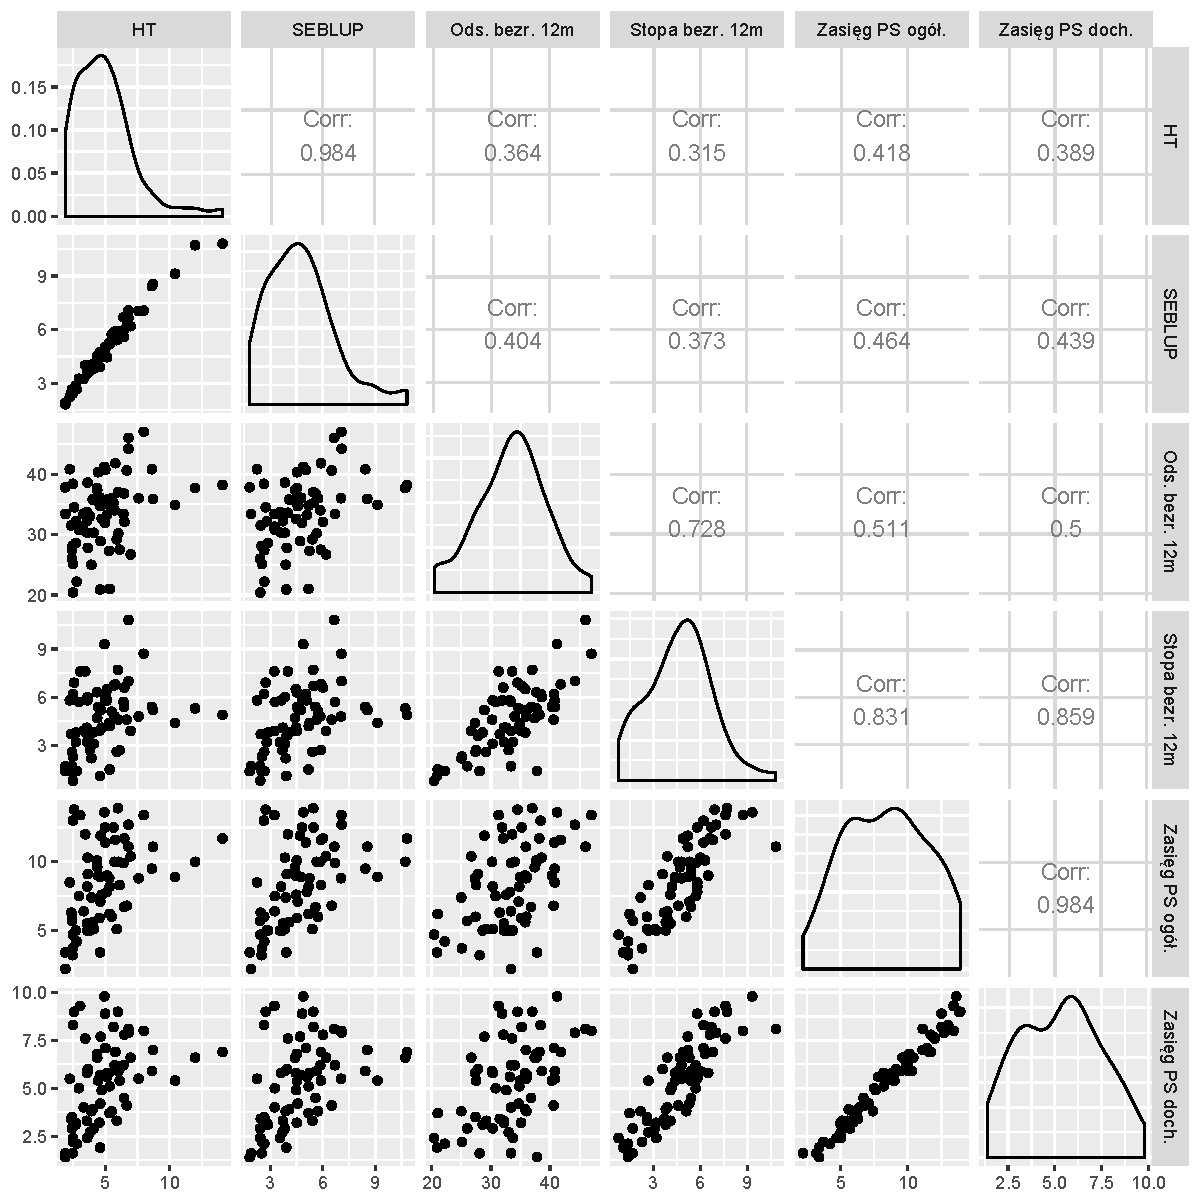
\includegraphics[width=0.8\textwidth]{05_wykresy/pgi_podreg_por-1.pdf}\\
\small{Źródło: opracowanie własne na podstawie EU-SILC 2011 oraz BDL.}
\label{fig:pgi_podreg_por}
\end{figure}

\begin{figure}[ht]
\caption{Porównanie oszacowań głębokości ubóstwa z danymi pochodzącymi z rejestrów administracyjnych na poziomie powiatów}
\centering
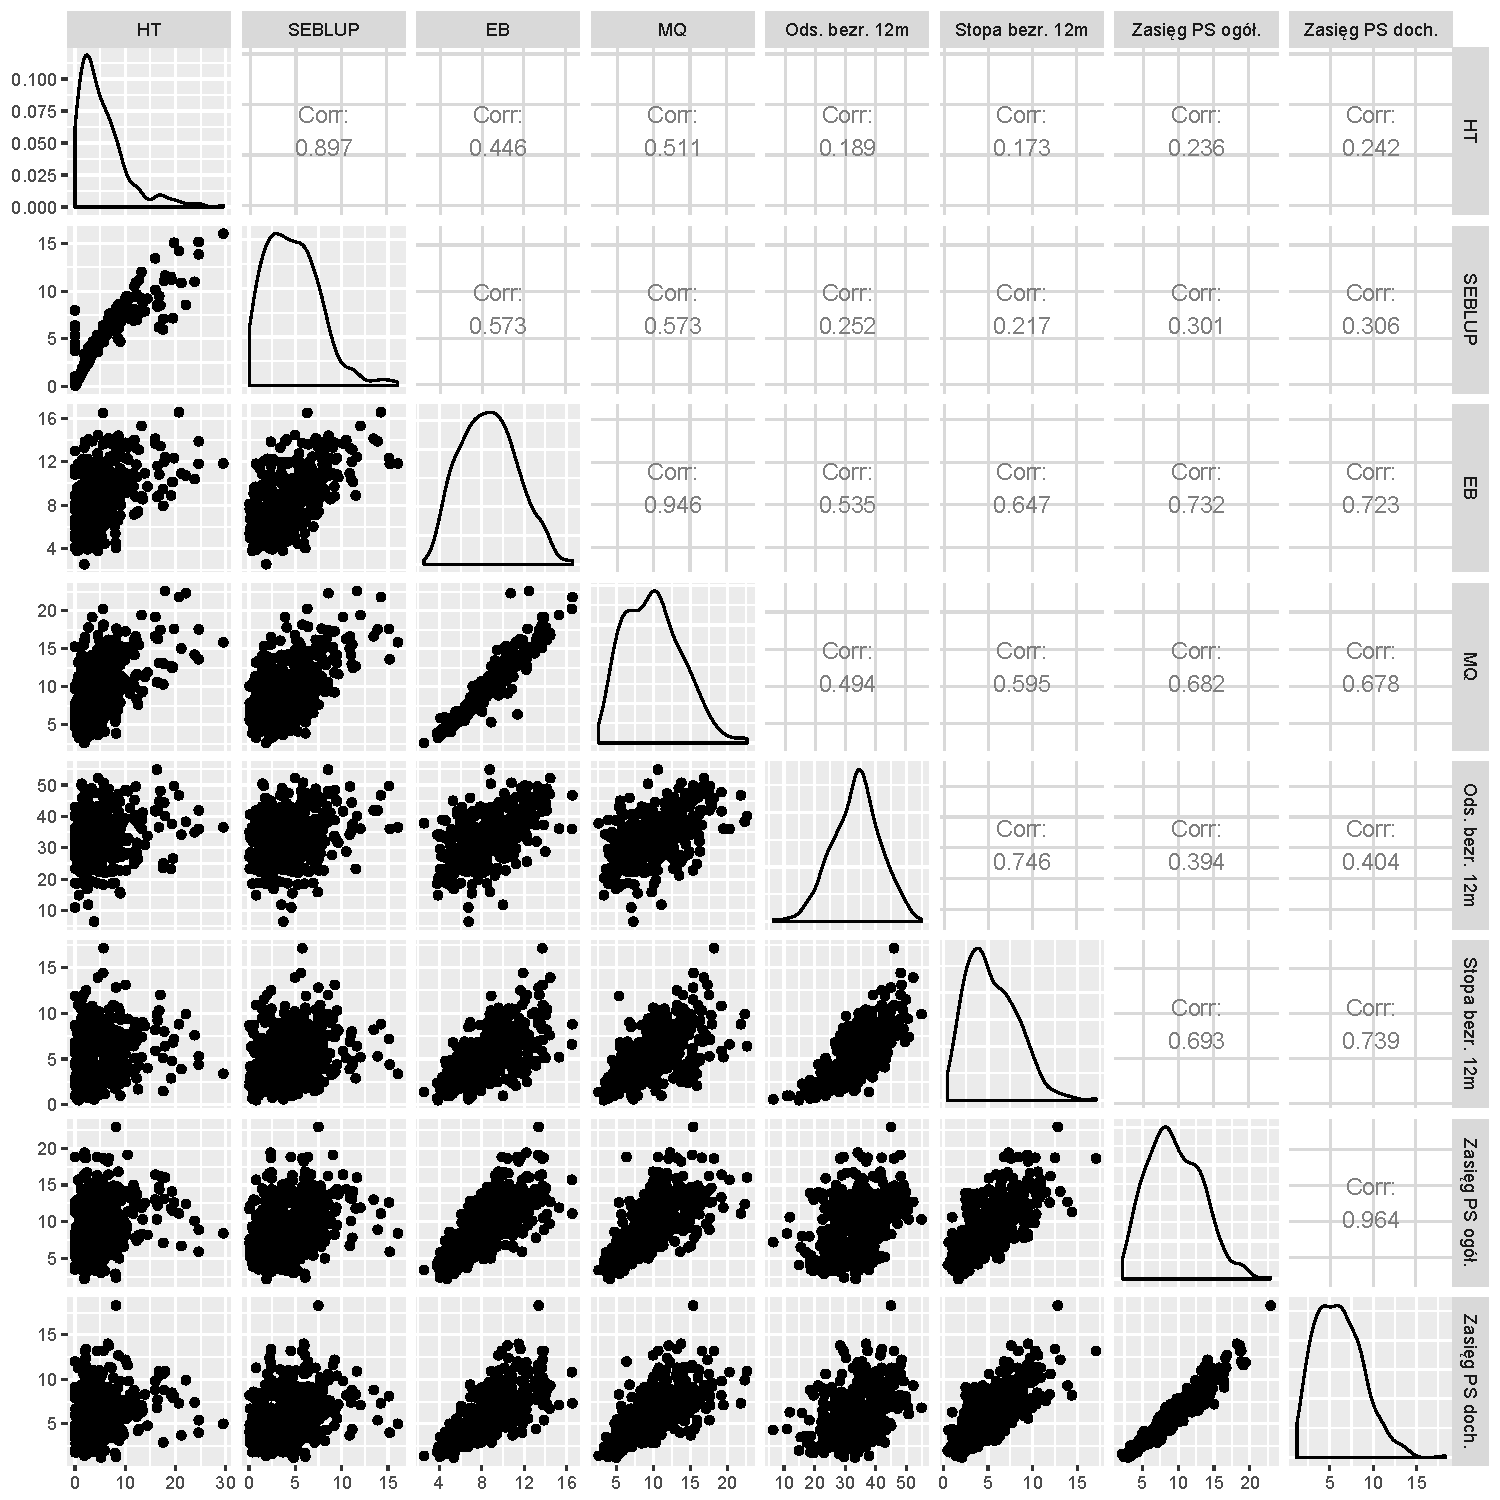
\includegraphics[width=0.8\textwidth]{05_wykresy/pgi_pow_por-1.pdf}\\
\small{Źródło: opracowanie własne na podstawie EU-SILC 2011, NSP 2011 oraz BDL.}
\label{fig:pgi_pow_por}
\end{figure}



\end{document}
